\documentclass[12pt,twoside]{report}

\usepackage[english]{babel}

\usepackage[nopostdot,  style=super, nonumberlist, toc]{glossaries}
\usepackage{tablefootnote}
\usepackage{supertabular}
\usepackage[utf8]{inputenc}
\usepackage{graphicx}
\usepackage{ngerman}
\usepackage[a4paper,width=150mm,top=25mm,bottom=25mm]{geometry}
\usepackage{fancyhdr}
\usepackage{titlesec}
\usepackage{hyperref}
\usepackage{float}
\usepackage{amsmath}
\usepackage{ulem}
\usepackage{multirow}
\usepackage{colortbl}
\usepackage{siunitx}
\usepackage{lscape}
\usepackage{listings}
\usepackage{xcolor}
\usepackage{url}
\usepackage{acronym}
\usepackage{graphicx}
\usepackage{pdfpages}
\usepackage{graphicx,subcaption}

\usepackage[numbers,sort&compress]{natbib}



% Generate the glossary
\makenoidxglossaries
 
%----------------------------------------------------------------------------------------
%	ABBREVIATIONS
%----------------------------------------------------------------------------------------
\setacronymstyle{long-short}

%Ein eigenes Symbolverzeichnis erstellen
\newglossary[slg]{abbreslist}{syi}{syg}{Abbreviations}
\newglossary[slg]{B2Blist}{syi}{syg}{Abbreviations related to FAIR B2B transfer system }
\newglossary[slg]{symbolslist}{syi}{syg}{Parameters related to synchrotron and beam}
\newglossary[slg]{B2B_sym_slist}{syi}{syg}{Parameters related to FAIR B2B transfer system}

%Befehle für Symbole
\newglossaryentry{symb:C_param}{
name=$C^{X}$,
description={Circumference of the extraction/injection orbit of a specific synchrotron},
sort=symbolpi, type=symbolslist
}

%\newglossaryentry{symb:C18}{
%name=$C^{SIS18}$,
%description={Circumference of the designed orbit of SIS18},
%sort=symbolpi, type=symbolslist
%}
%\newglossaryentry{symb:C100}{
%name=$C^{SIS100}$,
%description={Circumference of the designed orbit of SIS100},
%sort=symbolpi, type=symbolslist
%}
\newglossaryentry{symb:voltage}{
name=$u$,
description={Longitudinal accelerating voltage at rf cavity},
sort=symbolpi, type=symbolslist
}
\newglossaryentry{symb:amp_voltage}{
name=$V_0$,
description={Amplitude of the rf voltage},
sort=symbolpi, type=symbolslist
}
\newglossaryentry{symb:Syn_phase}{
name=$\phi_s$,
description={Synchronous phase},
sort=symbolphi, type=symbolslist
}
\newglossaryentry{symb:rf_freq1}{
name=$f_{\mathit{rf}}$,
description={Rf frequency},
sort=symbolphi, type=symbolslist
}

\newglossaryentry{symb:rev_freq1}{
name=$f_{\mathit{rev}}$,
description={Revolution frequency},
sort=symbolphi, type=symbolslist
}
\newglossaryentry{symb:harmonic}{
name=$h$,
description={Harmonic number},
sort=symbolphi, type=symbolslist
}
\newglossaryentry{symb:rev_freq}{
name=$f_{\mathit{rev}}^{X} $,
description={or $f_{h=1}^{X}$. Revolution frequency of a specific synchrotron}, 
sort=symbolpi, type=symbolslist
}
\newglossaryentry{symb:cavity_freq}{
name=$f_{\mathit{rf}}^{X}$,
description={or $f_{h=cavity\_harmonic}^{X}$. Cavity rf frequency of a specific synchrotron},
sort=symbolpi, type=symbolslist
}
\newglossaryentry{symb:bucket_freq}{
name=$f_\mathit{bucket}$,
description={Rf frequency of the bucket indication signal},
sort=symbolpi, type=symbolslist
}
\newglossaryentry{symb:harmonic_param}{
name=$h^X$,
description={Harmonic number of a specific synchrotron}, %$X=l$, harmonic number of large synchrotron; $X=s$, harmonic number of small synchrotron; $X=src$, harmonic number of source synchrotron; $X=trg$, harmonic number of target synchrotron },
sort=symbollambda, type=symbolslist
}

\newglossaryentry{symb:period_rf}{
name=$T_{rf}^{X}$,
description={Period of the cavity rf frequency of machine X},
sort=symbolpi, type=symbolslist
}
\newglossaryentry{symb:period_rev}{
name=$T_{rev}^{X}$,
description={Period of the revolution period of machine X},
sort=symbolpi, type=symbolslist
}


\newglossaryentry{symb:period_18h1}{
name=$T_{h=1}^{SIS18}$,
description={Revolution period of SIS18},
sort=symbolpi, type=symbolslist
}
\newglossaryentry{symb:period_18h2}{
name=$T_{h=2}^{SIS18}$,
description={Rf period of the h=2 cavity rf frequency of SIS18},
sort=symbolpi, type=symbolslist
}
%\newglossaryentry{symb:100h1}{
%name=$f_{h=1}^{SIS100}$,
%description={RF cavity revolution frequency of SIS100},
%sort=symbolpi, type=symbolslist
%}
%\newglossaryentry{symb:100h10}{
%name=$f_{h=10}^{SIS100}$,
%description={RF cavity driving frequency of SIS100},
%sort=symbolpi, type=symbolslist
%}
\newglossaryentry{symb:period_100h1}{
name=$T_{h=1}^{SIS100}$,
description={Revolution period of SIS100},
sort=symbolpi, type=symbolslist
}
\newglossaryentry{symb:rest_mass}{
name=$m_0$,
description={Rest mass},
sort=symbolpi, type=symbolslist
}
\newglossaryentry{symb:period_100h10}{
name=$T_{h=10}^{SIS100}$,
description={Rf period of the h=10 cavity rf frequency of SIS100},
sort=symbolpi, type=symbolslist
}


%\newglossaryentry{symb:start_phase}{
%name=$t_0$,
%description={Start time of the rf frequency modulation for the phase shift method},
%sort=symbolpi, type=symbolslist
%}

\newglossaryentry{symb:syn_phase0}{
name=$\Delta \phi_{\mathit{s\_0}}$,
description={synchronous phase with no frequency modulation},
sort=symbolphi, type=symbolslist
}

\newglossaryentry{symb:bucket_size}{
name=$\alpha_b$,
description={Bucket area factor},
sort=symbollambda, type=symbolslist
}
\newglossaryentry{symb:an_freq_syn}{
name=$\omega_s$,
description={Angular synchrotron frequency},
sort=symbollambda, type=symbolslist
}
\newglossaryentry{symb:an_freq_syn0}{
name=$\omega_{\mathit{syn\_0}}$,
description={Angular synchrotron frequency with no frequency modulation},
sort=symbollambda, type=symbolslist
}

\newglossaryentry{symb:mom_factor}{
name=$\alpha_p$,
description={Momentum compaction factor},
sort=symbollambda, type=symbolslist
}
\newglossaryentry{symb:s_syn_phase}{
name=$\phi_s$,
description={Synchronous phase},
sort=symbollambda, type=symbolslist
}

\newglossaryentry{symb:chromaticity_x}{
name=$Q^\prime_x$,
description={Horizontal chromaticity},
sort=symbollambda, type=symbolslist
}
\newglossaryentry{symb:chromaticity_y}{
name=$Q^\prime_y$,
description={Vertical chromaticity},
sort=symbollambda, type=symbolslist
}
\newglossaryentry{symb:chromaticity_x_y}{
name=$Q^\prime_{\mathit{x/y}}$,
description={Horizontal/vertical chromaticity},
sort=symbollambda, type=symbolslist
}
\newglossaryentry{symb:oscillation_x}{
name=$Q_x$,
description={Horizontal tune},
sort=symbollambda, type=symbolslist
}
\newglossaryentry{symb:oscillation_y}{
name=$Q_y$,
description={Vertical tune},
sort=symbollambda, type=symbolslist
}
\newglossaryentry{symb:oscillation_x_y}{
name=$Q_{\mathit{x/y}}$,
description={Horizontal/vertical tune},
sort=symbollambda, type=symbolslist
}
\newglossaryentry{symb:c_chromaticity_x}{
name=$\Delta Q_x$,
description={Horizontal tune shift},
sort=symbollambda, type=symbolslist
}
\newglossaryentry{symb:c_chromaticity_y}{
name=$\Delta Q_y$,
description={Vertical tune shift},
sort=symbollambda, type=symbolslist
}
\newglossaryentry{symb:c_chromaticity_x_y}{
name=$\Delta Q_{\mathit{x/y}}$,
description={Horizontal/vertical tune shift},
sort=symbollambda, type=symbolslist
}

\newglossaryentry{symb:adiabaticity}{
name=$\varepsilon$,
description={Adiabaticity parameter},
sort=symbollambda, type=symbolslist
}


\newglossaryentry{symb:syn_freq}{
name=$\omega_s(t)$,
description={Small-amplitude synchrotron frequency},
sort=symbollambda, type=symbolslist
}

%\newglossaryentry{symb:voltage1}{
%name=V(t),
%description={rf accelerating voltage},
%sort=symbollambda, type=symbolslist
%}
\newglossaryentry{symb:mgenet}{
name=$B$,
description={Magnetic field},
sort=symbollambda, type=symbolslist
}
\newglossaryentry{symb:transition_energy}{
name=$\gamma_t$,
description={Transition energy},
sort=symbollambda, type=symbolslist
}
\newglossaryentry{symb:relative_fac}{
name=$\gamma$,
description={Relativistic factor, which measures the total particle energy, $E$, in units of the particle rest energy, $E_0$},
sort=symbollambda, type=symbolslist
}

\newglossaryentry{symb:charge}{
name=$q$,
description={Charge of a particle},
sort=symbollambda, type=symbolslist
}
\newglossaryentry{symb:force}{
name=F(t),
description={Force},
sort=symbollambda, type=symbolslist
}
\newglossaryentry{symb:total_energy}{
name= $E$,
description={Total particle energy},
sort=symbollambda, type=symbolslist
}
\newglossaryentry{symb:rest_energy}{
name=$E_0$,
description={Particle rest energy},
sort=symbollambda, type=symbolslist
}

\newglossaryentry{symb:c}{
name=$c$,
description={Speed of the light},
sort=symbollambda, type=symbolslist
}
\newglossaryentry{symb:b}{
name=$\beta$,
description={Relative speed to the speed of light},
sort=symbollambda, type=symbolslist
}
\newglossaryentry{symb:velocity}{
name=$\upsilon(t)$,
description={Velocity of particle},
sort=symbollambda, type=symbolslist
}



\newglossaryentry{symb:R}{
name=$R$,
description={Orbit radius},
sort=symbollambda, type=symbolslist
}
\newglossaryentry{symb:P}{
name=$p$,
description={Particle momentum},
sort=symbollambda, type=symbolslist
}
\newglossaryentry{symb:f}{
name=f(t),
description={Revolution frequency},
sort=symbollambda, type=symbolslist
}
\newglossaryentry{symb:B}{
name=B(t),
description={Magnetic field},
sort=symbollambda, type=symbolslist
}
\newglossaryentry{symb:slip_fac}{
name=$\eta$,
description={Phase-slip factor},
sort=symbollambda, type=symbolslist
}

\newglossaryentry{symb:mom_comp}{
name=$\alpha_p$,
description={Momentum compaction factor},
sort=symbollambda, type=symbolslist
}

\newglossaryentry{symb:bending_rad}{
name=$\rho$,
description={Bending radius of a particle immersed in a magnetic field B},
sort=symbollambda, type=symbolslist
}
% Symbol for B2B transfer system
%\newglossaryentry{symb:integer}{
%name=$\kappa$,
%description={Integer, $m$ and $n$ are also integer},
%sort=symbolpi, type=B2B_sym_slist
%}
%\newglossaryentry{symb:decimal}{
%name=$\lambda$,
%description={Decimal},
%sort=symbolpi, type=B2B_sym_slist
%}
%\newglossaryentry{symb:18h1}{
%name=$f_{h=1}^{SIS18}$,
%description={RF cavity revolution frequency of SIS18},
%sort=symbolpi, type=B2B_sym_slist
%}
%\newglossaryentry{symb:18h2}{
%name=$f_{h=2}^{SIS18}$,
%description={RF cavity driving frequency of SIS18},
%sort=symbolpi, type=B2B_sym_slist
%}
\newglossaryentry{symb:GCD}{
name=$Y$,
description={Greatest common divisor},
sort=symbolpi, type=B2B_sym_slist
}
\newglossaryentry{symb:pha_shift}{
name=$\Delta \phi$,
description={Target phase shift for the phase shift method. Bunch-to-bucket injection center mismatch for the frequency beating method},
sort=symbolpi, type=B2B_sym_slist
}
\newglossaryentry{symb:pha_shift_rf}{
name=$\Delta \phi_\mathit{rf}$,
description={Phase difference between two cavity rf frequencies for the phase shift method, Bunch-to-bucket injection center mismatch within the synchronization window for the frequency beating method},
sort=symbolpi, type=B2B_sym_slist
}
\newglossaryentry{symb:pha_shift_syn}{
name=$\Delta \phi_\mathit{syn}$,
description={Phase difference between two synchronization frequencies for the phase shift method, phase mismatch  between two synchronization frequencies within the synchronization window for the frequency beating method},
sort=symbolpi, type=B2B_sym_slist
}
\newglossaryentry{symb:pha_shift_shift}{
name=$\Delta \phi_\mathit{shift}$,
description={Required phase shift for the Group DDS with the synchronization frequency},
sort=symbolpi, type=B2B_sym_slist
}
\newglossaryentry{symb:pha_step}{
name=$\Delta \phi_\mathit{step}$,
description={Arithmetic increasing phase of the phase difference between two cavity rf frequencies for the frequency beating},
sort=symbolpi, type=B2B_sym_slist
}
\newglossaryentry{symb:freq_modulation}{
name=$\Delta f_\mathit{rf}$,
description={Rf frequency modulation on the cavity rf frequency for the phase shift method, rf frequency detune on the cavity rf frequency for the frequency beating method},
sort=symbolpi, type=B2B_sym_slist
}
\newglossaryentry{symb:freq_modulation1}{
name=$\Delta f_\mathit{syn}$,
description={Rf frequency modulation on the synchronization frequency for the phase shift method, rf frequency detune on the synchronization frequency for the frequency beating method},
sort=symbolpi, type=B2B_sym_slist
}
\newglossaryentry{symb:period_phase}{
name=$T$,
description={Duration of rf frequency modulation for the phase shift method },
sort=symbolpi, type=B2B_sym_slist
}
\newglossaryentry{symb:inital_phase}{
name=$\Delta \varphi$,
description={Phase step growth because of the frequency beating},
sort=symbollambda, type=B2B_sym_slist
} 
\newglossaryentry{symb:best_align}{
name=$t_{best}$,
description={Best estimate of alignment of zero crossing points of Reference RF Signals of source and target synchrotrons},
sort=symbollambda, type=B2B_sym_slist
}
\newglossaryentry{symb:delay_com}{
name=$t_\mathit{delay}$,
description={Delay compensation for the TOF, all propagation delays, the kicker preparation time and the bucket pattern},
sort=symbollambda, type=B2B_sym_slist
}
\newglossaryentry{symb:probable_aligh}{
name=$\delta t_{best}$,
description={Uncertainty of the best estimate of alignment of zero crossing points of Reference RF Signals of source and target synchrotrons},
sort=symbollambda, type=B2B_sym_slist
}
\newglossaryentry{symb:slope}{
name=$k^X$,
description={Slope of the phase deviation between the Synchronization Reference Signal and a dedicated Reference RF Signal of the synchrotron X},
sort=symbolpi, type=B2B_sym_slist
}

\newglossaryentry{symb:h1phase100}{
name=$\psi_{h=1}^{SIS100}$,
description={Predicted SIS100 h=1 rf phase at $t_{\psi}$},
sort=symbollambda, type=B2B_sym_slist
}
\newglossaryentry{symb:h15phase18}{
name=$\psi_{h=1/5}^{SIS18}$,
description={Predicted SIS18 h=1/5 rf phase at $t_{\psi}$ },
sort=symbollambda, type=B2B_sym_slist
}
\newglossaryentry{symb:un_h1phase100}{
name=$\delta \psi_{h=1}^{SIS100}$,
description={Uncertainty of the predicted SIS100 rf phase at h=1 },
sort=symbollambda, type=B2B_sym_slist
}
\newglossaryentry{symb:un_h15phase18}{
name=$\delta \psi_{h=1/5}^{SIS18}$,
description={Uncertainty of the predicted SIS18 rf phase at h=1/5 },
sort=symbollambda, type=B2B_sym_slist
}
\newglossaryentry{symb:h10phase100}{
name=$\phi_{h=10}^{SIS100}$,
description={Phase at the h=10 cavity rf frequency of SIS100 at $t_{\psi}$},
sort=symbollambda, type=B2B_sym_slist
}
\newglossaryentry{symb:h2phase18}{
name=$\phi_{h=2}^{SIS18}$,
description={Phase at the h=2 cavity rf frequency of SIS18 at $t_{\psi}$  },
sort=symbollambda, type=B2B_sym_slist
}
\newglossaryentry{symb:un_h10phase100}{
name=$\delta \phi_{h=10}^{SIS100}$,
description={Uncertainty of rf phase at the h=10 cavity rf frequency of SIS100 },
sort=symbollambda, type=B2B_sym_slist
}
\newglossaryentry{symb:un_h2phase18}{
name=$\delta \phi_{h=2}^{SIS18}$,
description={Uncertainty of rf phase at the h=2 cavity rf frequency of SIS18  },
sort=symbollambda, type=B2B_sym_slist
}
\newglossaryentry{symb:prediction_time}{
name=$t_{\psi}$,
description={Time of the predicted phase},
sort=symbollambda, type=B2B_sym_slist
}
\newglossaryentry{symb:uncertainty_time}{
name=$\delta t_{\psi}$,
description={Uncertainty of the predicted phase advance at time domain},
sort=symbollambda, type=B2B_sym_slist
}
\newglossaryentry{symb:upper_Ttime}{
name=$T_{phase\_ shift}^{upper\_ bound}$,
description={Upper bound time of the phase shift process},
sort=symbollambda, type=B2B_sym_slist
}

\newglossaryentry{symb:un_upper_time_phase_shift}{
name=$\delta T_{phase\_ shift}^{upper\_ bound}$,
description={Uncertainty of the upper bound time of the phase shift process},
sort=symbollambda, type=B2B_sym_slist
}

\newglossaryentry{symb:phase_just_frequency_beating}{
name=$\Delta \phi_{adjustment}$,
description={Phase adjustment of the frequency beating method, calculated by B2B source SCU},
sort=symbollambda, type=B2B_sym_slist
}
\newglossaryentry{symb:phase_s_alignment}{
name=$\psi_{s\_alignment}$,
description={Rf phase of the cavity driving frequency at the start of the probable rang of alignment},
sort=symbollambda, type=B2B_sym_slist
}
\newglossaryentry{symb:win_correction}{
name=$\Delta t_{win \_correct}$,
description={Time correction for the start of the probable range of alignment [$t_{best}$-$\delta t_{best}$,$t_{best}$+$\delta t_{best}$] to the best estimate of the start of the synchronization window},
sort=symbollambda, type=B2B_sym_slist
}
\newglossaryentry{symb:win_start}{
name=$t_\mathit{w\_start}$,
description={Start of the synchronization window, calculated by B2B source SCU},
sort=symbollambda, type=B2B_sym_slist
}
\newglossaryentry{symb:G}{
name=$G$,
description={Bunch gap},
sort=symbollambda, type=B2B_sym_slist
}
\newglossaryentry{symb:L}{
name=$L$,
description={Distance from the leftmost to the rightmost SIS18 extraction/SIS100 injection kicker unit},
sort=symbollambda, type=B2B_sym_slist
}
\newglossaryentry{symb:d}{
name=$d$,
description={Distance between two extraction kicker crates of SIS18},
sort=symbollambda, type=B2B_sym_slist
}
\newglossaryentry{symb:D}{
name=$D$,
description={Sum distance of d and the 2nd crate},
sort=symbollambda, type=B2B_sym_slist
}
\newglossaryentry{symb:t_b2b}{
name=$t_\mathit{B2B}$,
description={Start time of the B2B transfer},
sort=symbollambda, type=B2B_sym_slist
}
\newglossaryentry{symb:d_t}{
name=$\Delta t$,
description={Beating time for the synchronization},
sort=symbollambda, type=B2B_sym_slist
}
\newglossaryentry{symb:phase_shift_actual}{
name=$f_{actual}$ ,
description={Actual rf frequency modulation profile, calculated by PSM},
sort=symbollambda, type=B2B_sym_slist
} 
\newglossaryentry{symb:phase_shift_normalized}{
name=$f_{normalized}$ ,
description={Normalized rf frequency modulation profile, preloaded from SM},
sort=symbollambda, type=B2B_sym_slist
}
\newglossaryentry{symb:ext_pre}{
name=$t_{ext}$ ,
description={Extraction kicker delay},
sort=symbollambda, type=B2B_sym_slist
}
\newglossaryentry{symb:inj_pre}{
name=$t_{inj}$ ,
description={Injection kicker delay},
sort=symbollambda, type=B2B_sym_slist
}
\newglossaryentry{symb:diff_sync}{
name=$t_{\mathit{diff\_sync}}$ ,
description={Target time difference between rf systems of two synchrotrons in the format of time},
sort=symbollambda, type=B2B_sym_slist
}
\newglossaryentry{symb:two_TOF}{
name=$t_{\mathit{TOF}}$,
description={Time-of-Flight between two synchrotrons},
sort=symbollambda, type=B2B_sym_slist
}

\newglossaryentry{symb:bucket_pattern}{
name=$t_{\mathit{bucket}}$ ,
description={Time delay for a specific bucket pattern},
sort=symbollambda, type=B2B_sym_slist
}
\newglossaryentry{symb:tsrc}{
name=$t_{v\_ext}$,
description={Time corresponding to the distance between the virtual rf cavity and the extraction position of the source synchrotron},
sort=symbollambda, type=B2B_sym_slist
}
\newglossaryentry{symb:ttrg}{
name=$t_{v\_inj}$,
description={Time corresponding to the distance between the virtual rf cavity and the injection position of the target synchrotron},
sort=symbollambda, type=B2B_sym_slist
}
\newglossaryentry{symb:temg}{
name=$t_{v\_emg}$,
description={Time corresponding to the distance between the virtual rf cavity and the emergency extraction position of SIS100},
sort=symbollambda, type=B2B_sym_slist
}
\newglossaryentry{symb:Demg}{
name=$t_{emg}$,
description={Extraction kicker delay of SIS100 for the emergency kick},
sort=symbollambda, type=B2B_sym_slist
}
\newglossaryentry{symb:mismatch}{
name=$\Delta \theta$,
description={Mismatch between the bunch and bucket center},
sort=symbollambda, type=B2B_sym_slist
}
\newglossaryentry{symb:syn_win_length}{
name=$T_{w}$,
description={Length of the synchronization window},
sort=symbollambda, type=B2B_sym_slist
}
\newglossaryentry{symb:phase_diff}{
name=$\Delta \varphi^X$,
description={Measured phase deviation between the Reference RF Signal and the Synchronization Reference Signal of the synchrotron X by PAM module},
sort=symbollambda, type=B2B_sym_slist
}

\newglossaryentry{symb:phase_diff_T0}{
name=$\psi^X$,
description={Extrapolated phase advance between the Reference RF Signal and the Synchronization Reference Signal of the synchrotron X by PAP module},
sort=symbollambda, type=B2B_sym_slist
}
\newglossaryentry{symb:synchronization_freq}{
name=$f_\mathit{syn}^{X}$,
description={Synchronization frequency},
sort=symbollambda, type=B2B_sym_slist
}
\newglossaryentry{symb:synchronization_freq_period}{
name=$T_\mathit{syn}^{X}$,
description={Rf period of synchronization frequency},
sort=symbollambda, type=B2B_sym_slist
}

\newglossaryentry{symb:phase_diff_t_T0}{
name=$\psi2$,
description={Extrapolated phase advance between the Reference RF Signal and the Synchronization Reference Signal of the target synchrotron by PAP module},
sort=symbollambda, type=B2B_sym_slist
}
\newglossaryentry{symb:time_phase_diff_T0}{
name=$t_{\psi}^X$,
description={Timestamp corresponding to the extrapolated phase advance $\psi^X$},
sort=symbollambda, type=B2B_sym_slist
}
\newglossaryentry{symb:initial_phase advance}{
name=$\psi_0$,
description={Initial phase advance in a linear relationship between the phase advance and time of the target synchrotron},
sort=symbollambda, type=B2B_sym_slist
}

\newglossaryentry{symb:beating_freq}{
name=$\Delta f$,
description={Beating frequency between two synchronization frequencies},
sort=symbollambda, type=B2B_sym_slist
}
\newglossaryentry{symb:syn_ref}{
name=$f_{\mathit{syn}}^{\mathit{REF}}$,
description={Frequency of the Synchronization Reference Signal},
sort=symbolphi, type=B2B_sym_slist
}
\newglossaryentry{symb:B2B_ref}{
name=$f_\mathit{B2B}^\mathit{X}$,
description={Frequency of the specified Reference RF Signal for the phase advance measurement},
sort=symbolphi, type=B2B_sym_slist
}

%Befehle für Abbreviation
\newglossaryentry{GCD}
{
name={GCD},
description={Greatest Common Divisor},type=abbreslist
}
\newglossaryentry{TOF}
{
name={TOF},
description={Time-Of-Flight},type=abbreslist
}
\newglossaryentry{B2B}
{
name={B2B},
description={Bunch-to-bucket},type=abbreslist
}
\newglossaryentry{GMT}{
name={GMT},
description={General Machine Timing},type=abbreslist
}
\newglossaryentry{API}{
name={API},
description={Application Programming Interface},type=abbreslist
}
\newglossaryentry{BuTiS}{
name={BuTiS},
description={Bunchphase Timing System},type=abbreslist
}

\newglossaryentry{BI}{
name={BI},
description={Beam Instrumentation},type=abbreslist
}
\newglossaryentry{CM}{
name={CM},
description={Clock Master},type=abbreslist
}
\newglossaryentry{MM}{
name={MM},
description={Management Master},type=abbreslist
}
\newglossaryentry{CCS}{
name={CCS},
description={Central Control System },type=abbreslist
}
\newglossaryentry{CR}{
name={CR},
description={Collector Ring at GSI},type=abbreslist
}
\newglossaryentry{DSP}{
name={DSP},
description={Digital Signal Processor},type=abbreslist
}
\newglossaryentry{DM}{name={DM},
description={Data Master},type=abbreslist
}
\newglossaryentry{ESR}{
name={ESR},
description={Experimental Storage Ring at GSI},type=abbreslist
}
\newglossaryentry{UNILAC}{
name={UNILAC},
description={Universal Linear Accelerator at GSI},type=abbreslist
}
\newglossaryentry{FRS}{
name={FRS},
description={Fragment Separator},type=abbreslist
}
\newglossaryentry{PBHV}{
name={PBHV},
description={Primary Beam High Voltage},type=abbreslist
}
\newglossaryentry{PBRF}{
name={PBRF},
description={Primary Beam Radio Frequency},type=abbreslist
}
\newglossaryentry{Pbar}{
name={Pbar},
description={Proton bar},type=abbreslist
}

\newglossaryentry{SBES}{
name={SBES},
description={Experimentierspeicherring ESR},type=abbreslist
}
\newglossaryentry{SHE-P}{
name={SHE-P},
description={SHE-Physik},type=abbreslist
}
\newglossaryentry{FAIR}{
name={FAIR},
description={Facility for Antiproton and Ion Research at GSI},type=abbreslist
}
\newglossaryentry{TM}{
name={TM},
description={Timing Master},type=abbreslist
}
\newglossaryentry{FEC}{
name={FEC},
description={Front End Controller},type=abbreslist
} 

\newglossaryentry{FESA}{
name={FESA},
description={Front-End software Architecture},type=abbreslist
}
\newglossaryentry{LSA}{
name={LSA},
description={LHC Software Architecture},type=abbreslist
}
\newglossaryentry{LHC}{
name={LHC},
description={Large Hadron Collider at CERN},type=abbreslist
}
\newglossaryentry{PSB}{
name={PSB},
description={Proton Synchrotron Booster at CERN},type=abbreslist
}
\newglossaryentry{RIB}{
name={RIB},
description={Rare Isotope Beams},type=abbreslist
}
\newglossaryentry{PS}{
name={PS},
description={Proton Synchrotron at CERN},type=abbreslist
}
\newglossaryentry{SPS}{
name={SPS},
description={Super Proton Synchrotron at CERN},type=abbreslist
}
\newglossaryentry{LEIR}{
name={LEIR},
description={Low Energy Ion Ring at CERN},type=abbreslist
}
\newglossaryentry{J-PARC}{
name={J-PARC},
description={Japan Proton Accelerator Complex},type=abbreslist
}
\newglossaryentry{RCS}{
name={RCS},
description={Rapid Cycle Synchrotron at J-PARC},type=abbreslist
}
\newglossaryentry{MR}{
name={MR},
description={Main Ring at J-PARC},type=abbreslist
}
\newglossaryentry{BNL}{
name={BNL},
description={Brookhaven National Laboratory},type=abbreslist
}
\newglossaryentry{AGS}{
name={AGS},
description={Alternating Gradient Synchrotron at BNL},type=abbreslist
}
\newglossaryentry{RHIC}{
name={RHIC},
description={Relativistic Heavy Ion Collide at BNL},type=abbreslist
}
\newglossaryentry{IMP}{
name={IMP},
description={Institute of Modern Physics},type=abbreslist
}
\newglossaryentry{HIRFL}{
name={HIRFL},
description={Heavy Ion Research Facility at IMP},type=abbreslist
}
\newglossaryentry{SFC}{
name={SFC},
description={Sector Focusing Cyclotron at IMP},type=abbreslist
}
\newglossaryentry{SSC}{
name={SSC},
description={Separated Sector Cyclotron at IMP},type=abbreslist
}
\newglossaryentry{CSRm}{
name={CSRm},
description={Cooler Storage Ring main ring at IMP},type=abbreslist
}
\newglossaryentry{CSRe}{
name={CSRe},
description={Cooler Storage Ring experimental ring at IMP},type=abbreslist
}
\newglossaryentry{HESR}{
name={HESR},
description={High Energy Storage Ring at GSI},type=abbreslist
}
\newglossaryentry{LLRF}{
name={LLRF},
description={Low-level RF },type=abbreslist
}
\newglossaryentry{CSCO}{
name={CSCO},
description={Common Systems Control Systems},type=abbreslist
}

\newglossaryentry{MPS}{
name={MPS},
description={Machine Protection System},type=abbreslist
}
\newglossaryentry{NESR}{
name={NESR},
description={New Experimental Storage Ring at GSI},type=abbreslist
}

\newglossaryentry{RESR}{
name={RESR},
description={Recycled Experimental Storage Ring at GSI},type=abbreslist
}
\newglossaryentry{RF}{name={rf},
description={Radio Frequency},type=abbreslist
}
\newglossaryentry{SM}{name={SM},
description={Settings Management},type=abbreslist
}
\newglossaryentry{SIS18}{
name={SIS18},
description={SchwerIonen Synchrotron (18 Tm magnetic rigidity) at GSI},type=abbreslist
}
\newglossaryentry{SIS100}{
name={SIS100},
description={SchwerIonen Synchrotron (100 Tm magnetic rigidity) at GSI},type=abbreslist
}
\newglossaryentry{SIS300}{
name={SIS300},
description={SchwerIonen Synchrotron (300 Tm magnetic rigidity) at GSI},type=abbreslist
}
\newglossaryentry{VLAN}{
name={VLAN},
description={Virtual LAN},type=abbreslist
}
\newglossaryentry{WR}{
name={WR},
description={White Rabbit},type=abbreslist
}
\newglossaryentry{SCU}{
name={SCU},
description={Scalable Control Unit},type=abbreslist
}
\newglossaryentry{FPGA}{
name={FPGA},
description={Field Programmable Gate Array},type=abbreslist
}
\newglossaryentry{TTL}{
name={TTL},
description={Transistor–Transistor Logic},type=abbreslist
}
\newglossaryentry{PC}{
name={PC},
description={Personal Computer},type=abbreslist
}
\newglossaryentry{CPU}{
name={CPU},
description={Central Processing Unit},type=abbreslist
}
\newglossaryentry{PAM}{
name={PAM},
description={Phase Advance Measurement module},type=B2Blist
}
\newglossaryentry{PAP}{
name={PAP},
description={Phase Advance Prediction module},type=B2Blist
}

\newglossaryentry{PSM}{
name={PSM},
description={Phase Shift Module},type=B2Blist
}
\newglossaryentry{PCM}{
name={PCM},
description={Phase Correction Module},type=B2Blist
}
\newglossaryentry{SR}{
name={SR},
description={Signal Reproduction module},type=B2Blist
}
\newglossaryentry{TD}{
name={TD},
description={Trigger Decision module},type=B2Blist
}
\newglossaryentry{FID}{
name={FID},
description={Format ID},type=abbreslist
}
\newglossaryentry{GID}{
name={GID},
description={Group ID},type=abbreslist
}
\newglossaryentry{BPID}{
name={BPID},
description={Beam Process ID},type=abbreslist
}
\newglossaryentry{FBAS}{
name={FBAS},
description={Fast Beam Abort System},type=abbreslist
}
\newglossaryentry{CERN}{
name={CERN},
description={Conseil Europ$\acute{e}$en pour la Recherche Nucl$\acute{e}$aire},type=abbreslist
}
\newglossaryentry{GSI}{
name={GSI},
description={GSI Helmholtzzentrum f$\ddot{u}$r Schwerionenforschung},type=abbreslist
}
\newglossaryentry{IP}{
name={IP},
description={Internet Protocol},type=abbreslist
} 
\newglossaryentry{Fermilab}{
name={Fermilab},
description={Fermi National Accelerator Laboratory},type=abbreslist
}
\newglossaryentry{DDS}{
name={DDS},
description={Direct Digital Synthesizer},type=abbreslist
}

\newglossaryentry{GUI}{
name={GUI},
description={Graphical  User Interface},type=abbreslist
}

%Befehle für Glossary

% Generate the glossary
\makenoidxglossaries

\newglossaryentry{glos:bucket_pattern}{
name={bucket pattern},
description={Rules for the buckets to be filled}
}
\newglossaryentry{glos:cir_ratio}{
name={circumference ratio},
description={Ratio of the circumference for synchrotrons of different size}
}
\newglossaryentry{glos:rev_ratio}{
name={revolution frequency ratio},
description={Ratio of the revolution frequencies for synchrotrons of different size}
}
\newglossaryentry{glos:har_ratio}{
name={harmonic ratio},
description={Cavity harmonic ratio between two synchrotrons}
}
\newglossaryentry{glos:bunch}{
name={bunch},
description={Collection of particles captured within one rf bucket}
}
\newglossaryentry{glos:ext_kick}{
name={extraction kicker},
description={Diverts a circulating beam to leave a synchrotron}
}
\newglossaryentry{glos:inj_kick}{
name={injection kicker},
description={Merges one beam into a circulating beam in a synchrotron }
}
\newglossaryentry{glos:rise_time}{
name={kicker rise time},
description={A period of time for kicker magnet to reach a stable magnetic field}
}
\newglossaryentry{glos:flat-top}{
name={kicker flat-top},
description={A period of time of kicker magnet with a stable magnetic field}
}
\newglossaryentry{glos:fall_time}{
name={kicker fall time},
description={A period of time of kicker magnet to reduce to zero magnetic field}
}
\newglossaryentry{glos:stationary_bucket}{
name={stationary rf bucket},
description={Rf system provides a region in the longitudinal phase space, within which all particles oscillate around the synchronous particle and stay together without energy gain/loss per turn (short: bucket)}
}
\newglossaryentry{glos:adia}{
name={adiabaticity},
description={Rf frequency is changed slowly enough for the beam to follow}
}
\newglossaryentry{glos:harmonic_number}{
name={harmonic number},
description={Integer ratio between the rf frequency and the revolution frequency}
}
\newglossaryentry{glos:syn_motion}{
name={synchrotron motion},
description={Oscillation of asynchronous particles around the synchronous particle}
}
\newglossaryentry{glos:bucket_size}{
name={bucket size},
description={Area in longitudinal phase space plane enclosed by the bucket}
}
\newglossaryentry{glos:bucket_height}{
name={bucket height},
description={Maximum momentum deviation of the rf bucket}
}
\newglossaryentry{glos:long_emi}{
name={longitudinal emittance},
description={Area occupied by a bunch in the longitudinal phase space plane}
}
\newglossaryentry{glos:bucket_area_factor}{
name={bucket area factor},
description={Ratio of bucket size of a running bucket to a stationary bucket}
}
\newglossaryentry{glos:running_bucket}{
name={running rf bucket},
description={Rf system provides a region in the longitudinal phase space, within which all particles oscillate around the synchronous particle and stay together with energy gain/loss per turn}
}
\newglossaryentry{glos:syn_particle}{
name={synchronous particle},
description={A particle who always sees a constant rf phase at the rf cavity}
}
\newglossaryentry{glos:tune}{
name={tune},
description={Number of particle trajectory oscillations during one revolution in the ring (transverse and longitudinal)}
}

\newglossaryentry{glos:uncertainty}{
name={uncertainty},
description={A non-negative parameter characterizing the dispersion of the values attributed to a measured quantity}
}
\newglossaryentry{glos:error_pro}{
name={error propagation},
description={Uncertainties in the original measurements ``propagate`` through calculations to cause uncertainties in the calculated final answers}
}

\newglossaryentry{glos:Rrf}{
name={Reference RF Signal},
description={Harmonic or subharmonic signal generated by the Group DDS and transmitted to the individual rf station as a reference signal},
}

\newglossaryentry{glos:group_DDS}{
name={Group DDS},
description={DDS module that generates an Reference RF Signal for a group of cavities}
}
\newglossaryentry{glos:cavity_DDS}{
name={Cavity DDS},
description={Cavity DDS provides rf signal for cavities}
}
\newglossaryentry{glos:vit_DDS}{
name={virtual rf cavity},
description={A virtual position around the ring, to which the Reference RF Signal corresponds}
}
\newglossaryentry{glos:timing_frame}{
name={timing frame},
description={A specific Ethernet frame with 110 byte frame length, which contains one timing message}
}
\newglossaryentry{glos:coarse_syn}{
name={coarse synchronization},
description={Bunches are transferred into buckets with the bunch-to-bucket center mismatch smaller than the upper bound}
}
\newglossaryentry{glos:fine_syn}{
name={fine synchronization},
description={Bunches are transferred into correct buckets}
}

\newglossaryentry{glos:Syn_ref_signal}{
name={Synchronization Reference Signal},
description={Shared synchronous reference signal at each supply room (same frequency and in phase)}
}
\newglossaryentry{glos:Syn_fre}{
name={synchronization frequencies},
description={An integral multiple of the derived rf frequency, which is the division of the revolution frequency. It is used for the phase alignment of two rf systems}
}

\newglossaryentry{glos:accuracy}{
name={accuracy of the start\\ of the synchronization window},
description={Time closeness of agreement between the observed and the best estimate start of the synchronization window, which is the sum of the precision and trueness}
}

\newglossaryentry{glos:precision}{
name={precision of the start\\ of the synchronization window},
description={Time closeness of agreement between the actual start of the synchronization window of different timing notes}
}
\newglossaryentry{glos:bucket_label}{
name={bucket indication signal},
description={Time indication of a dedicated bucket passing on the virtual rf cavity of the target synchrotron, when it is correct phase aligned with the rf system of the source synchrotron for the bunch-to-bucket injection}
}
\newglossaryentry{glos:T0_incidents}{
name={T0 incidents},
description={First positive zero-crossings of BuTiS C2 clocks after every BuTiS T0 edge}
}


\newglossaryentry{glos:trueness}{
name={trueness of the start\\ of the synchronization window},
description={Time closeness of agreement between the average actual start of the synchronization window of different timing notes and the best estimate start of the synchronization window}
}
\newglossaryentry{glos:frame_loss_rate}{
name={frame loss rate},
description={The ratio of the number of the lost Ethernet frames to the number of the theoretic received frames of a tested port}
}
\newglossaryentry{glos:latency}{
name={frame transfer latency},
description={The time interval between the frame reception and sending}
}
\newglossaryentry{glos:jitter}{
name={frame transfer jitter},
description={The time deviation between the transfer latencies of two consecutive frames}
}

\newglossaryentry{glos:broadcast}{
name={broadcast},
description={The frame is intended to be received and processed by every timing node on the WR network}
}
\newglossaryentry{glos:unicast}{
name={unicast},
description={The frame is intended to be received and processed by a specified timing node on the WR network}
}
\newglossaryentry{glos:trigger_scu}{
name={Trigger SCU},
description={Production of the trigger signal for kicker electronics},type=B2Blist
}

\newglossaryentry{glos:B2B_s_SCU}{
name={B2B source SCU},
description={Works as the B2B transfer master},type=B2Blist
}

\newglossaryentry{glos:B2B_master}{
name={B2B transfer master},
description={Responsible for the data collection of two synchrotrons, the data calculation, the data redistribution and the B2B transfer status check},type=B2Blist
}
\newglossaryentry{glos:B2B_t_SCU}{
name={B2B target SCU},
description={Collects the predicted phase of the target synchrotron and transfers it to the source synchrotron},type=B2Blist
}
\newglossaryentry{glos:machine_cycle}{
name={machine cycle},
description={One complete operation cycle of a machine, i.e. injection, ramp up, flattop, ejection and ramp down}
}
\newglossaryentry{glos:batch}{
name={batch},
description={A train of bunches circulating along a synchrotron to be transferred to buckets}% E.g. SIS100 batch: Train of 4 $\times$ 2 $U^{28+}$ bunches injected into SIS100 in one SIS18 to SIS100 super cycle. Or train of 4 $\times$ 1 $H^{+}$ bunches injected into SIS100 in one SIS18 to SIS100 super cycle}
}
\newglossaryentry{glos:bunch_gap}{
name={bunch gap},
description={Area without any bunches in a batch}
}
\newglossaryentry{glos:best_align}{
name={best estimate of alignment},
description={Fine time for the alignment of two RF Reference Signals}
}
\newglossaryentry{glos:pro_align}{
name={probable range of alignment},
description={Range within which the fine alignment lies because of the propagation of the uncertainty}
}

\lstset{tabsize=4, %
  frame=shadowbox, %把代码用带有阴影的框圈起来
  commentstyle=\color{red!50!green!50!blue!50},%浅灰色的注释
  rulesepcolor=\color{red!20!green!20!blue!20},%代码块边框为淡青色
  keywordstyle=\color{blue!90}\bfseries, %代码关键字的颜色为蓝色,粗体
  showstringspaces=false,%不显示代码字符串中间的空格标记
  stringstyle=\ttfamily, % 代码字符串的特殊格式
  keepspaces=true, %
  breakindent=22pt, %
  numbers=left,%左侧显示行号
  stepnumber=1,%
  numberstyle=\tiny, %行号字体用小号
  basicstyle=\footnotesize, %
  showspaces=false, %
  flexiblecolumns=true, %
  breaklines=true, %对过长的代码自动换行
  breakautoindent=true,%
  breakindent=4em, %
  escapebegin=\begin{CJK*}{GBK}{hei},escapeend=\end{CJK*},
  aboveskip=1em, %代码块边框
  %% added by http://bbs.ctex.org/viewthread.php?tid=53451
  fontadjust,
  captionpos=t,
  framextopmargin=2pt,framexbottommargin=2pt,abovecaptionskip=-3pt,belowcaptionskip=3pt,
  xleftmargin=4em,xrightmargin=4em, % 设定listing左右的空白
  texcl=true,
  % 设定中文冲突,断行,列模式,数学环境输入,listing数字的样式
  extendedchars=false,columns=flexible,mathescape=true
  % numbersep=-1em
}

\sisetup{per-mode=symbol,per-symbol = p}

\titleclass{\subsubsubsection}{straight}[\subsection]

\newcounter{subsubsubsection}[subsubsection]
\renewcommand\thesubsubsubsection{\thesubsubsection.\arabic{subsubsubsection}}
\renewcommand\theparagraph{\thesubsubsubsection.\arabic{paragraph}} % optional; useful if paragraphs are to be numbered

\titleformat{\subsubsubsection}
  {\normalfont\normalsize\bfseries}{\thesubsubsubsection}{1em}{}
\titlespacing*{\subsubsubsection}
{0pt}{3.25ex plus 1ex minus .2ex}{1.5ex plus .2ex}

\makeatletter
\renewcommand\paragraph{\@startsection{paragraph}{5}{\z@}%
  {3.25ex \@plus1ex \@minus.2ex}%
  {-1em}%
  {\normalfont\normalsize\bfseries}}
\renewcommand\subparagraph{\@startsection{subparagraph}{6}{\parindent}%
  {3.25ex \@plus1ex \@minus .2ex}%
  {-1em}%
  {\normalfont\normalsize\bfseries}}
\def\toclevel@subsubsubsection{4}
\def\toclevel@paragraph{5}
\def\toclevel@paragraph{6}
\def\l@subsubsubsection{\@dottedtocline{4}{7em}{4em}}
\def\l@paragraph{\@dottedtocline{5}{10em}{5em}}
\def\l@subparagraph{\@dottedtocline{6}{14em}{6em}}
\makeatother

\setcounter{secnumdepth}{4}
\setcounter{tocdepth}{4}
\pagestyle{fancy}

\renewcommand{\sectionmark}[1]{\markboth{\thesection.\ #1}{}}

\lhead{\bfseries \leftmark}
\chead{}
\rhead{}
%\lfoot{From: K. Grant}
%\cfoot{To: Dean A. Smith}
%\rfoot{\thepage}
\renewcommand{\headrulewidth}{0.4pt}
\renewcommand{\footrulewidth}{0.4pt}

\graphicspath{ {images/} }



\begin{document}

\pagenumbering{roman}
\begin{center}
\thispagestyle{empty}

    \vspace{6cm}
	 \LARGE \textbf{\uppercase{Development of the timing system for the Bunch-to-Bucket transfer between the FAIR accelerators }}
	 \vspace{2cm}
	%Thesis title

	{ \normalsize Vom Fachbereich\\
	Institut für Angewandte Physik\\
	der Goethe-Universit"at, Frankfurt am Main\\
	zur Erlangung des akademischen Grades\\
	eines Doktor der Naturwissenschaften\\
	genehmigte Dissertation\par}
    \vspace{2cm}
	%Author's name
    {\normalsize Von \par}
    \LARGE \textbf{ Jiaoni Bai}\\
    {\normalsize geboren am 9. November 1986 in Taiyuan, Shanxi Province, China \par}
    \vspace{2cm}
	\normalsize
	% referent
	\begin{align*}
		 \text{Referent: }\:  &\text{Prof. Dr. }\\
		 \text{Korreferent: }\: &\text{Prof. Dr.}\\
		 \text{Tag der Einreichung: }\: &\text{Date. Month Year}\\
		 \text{Tag der m"undlichen Pr"ufung: }\: &\text{Date. Month Year} \\
\end{align*}
	%Date
    \vspace{2cm}
    {\normalsize Darmstadt 2016}
\end{center}

\renewcommand{\labelitemii}{$\bullet$}

\clearpage
\vspace*{\fill}
\begin{center}
\begin{minipage}{.8\textwidth}
I would like to dedicate this dissertation to my dear parents,\\ loving husband and good friends ...
\end{minipage}
\end{center}
\vfill % equivalent to \vspace{\fill}
\clearpage

\chapter*{Acknowledgement}
First and foremost, I would like to thank my professor Prof. Oliver Kester. I have been so lucky to be his Ph.D. student. He gave me the chance to study at Goethe University, Frankfurt am Main and work in GSI for this interesting Ph.D. topic. It has been an honor to be his Ph.D. student. I appreciate all his contributions of time, ideas and funding to make my Ph.D. experience productive and stimulating. I was deeply influenced by his enthusiasm for his research and his selfless support for his students. I was thankful for his support, that I participated many international conferences, schools and workshops. This experience enriched my life and  
broadened my horizons.

I wish to express my sincere gratitude to Dr.David Ondreka and Dr.Dietrich Beck for their supervision, valuable guidance and helpful suggestions throughout my Ph.D. study. I have been greatly lucky to have so good supervisors, who cared much about my work and who answered my doubts patiently. They were like a lighthouse in the ocean, which guides me in the right direction. They are not only my  scientific supervisors, but also my mantor. They encouraged and motivated me during tough time of my Ph.D. They always told me ``Don't be frustrated and take it easy, everything will be fine.``. Hence, I will always keep a positive attitude and keep moving forward when I face with challenges, difficulties and temporary setbacks in the future.

I would like to acknowledge all colleagues in the timing group, CSCO department, GSI, Mathias Kreider, Stefan Rauch, Marcus Zweig, Alexander Hahn and former employee Dr. Wesley Terpstra, who provided me much technical support. I would like to extend my appreciation to department leader Dr.Ralph Baer, who gave much support for my Ph.D. topic. Thanks for their friendship and collaboration. I am especially grateful for the group member Cesar Prados, by whom I learned not only technical knowledge, but also how to work efficiently and how to become a good engineer. I would also like to thank Matthias Thieme, who provided me the devices for the test setup.  

I am also thankful for the good cooperation with Thibault Ferrand, who studies at Technische Universit$\ddot{a}$t Darmstadt and works in PBRF department, GSI. Thanks for his valuable contribution of the development of the LLRF system for the B2B transfer system for FAIR. I would like to extend my sincerest thanks and appreciation to PBRF department leader Prof. Harald Klingbeil for his support. In addition, a special thanks is also extended to Dr. Dieter Lens and Stefan Schaefer for their technical support. Thanks for Dr. Bernhard Zipfel to give me support about BuTiS.

I wish to express my sincere gratitude to SBES department leader Dr. Markus Steck for his technical support of ESR and CRYRING and Dr.Michael Block in SHE-P department for the supply of two SRS function generators. 

I must express my gratitude to GSI, who provides the Facility for Antiproton and Ion Research project for my experiment. And also HGS-HiRe, who provided the scholarship which allowed me to undertake this research.


Lastly, I would like to thank my family for all their love and encouragement. My parents always support me to pursuing my dreams. Most of all, my loving husband Zigao Li is so appreciated, whose always encourage me to realize my dreams. Thank you.

 \rightline{Jiaoni Bai}
 \rightline{Darmstadt, September 2016}





\chapter*{Abstract}
\addcontentsline{toc}{chapter}{Abstract}
The Facility for Antiproton and Ion Research (FAIR) is a new international particle accelerator facility under construction at GSI Helmholtz center for Heavy Ion Research GmbH. It is aiming at providing high-energy beams of ions from proton to uranium with high intensities, as well as beams of rare isotopes and beams of antiprotons. The existing facility at GSI includes the SIS18 and the ESR. The FAIR accelerator complex in its full version consists of many ring accelerators with different functionality. FAIR has synchrotrons (e.g. the SIS100), storage rings (e.g. the HESR) and collect rings (e.g. the CR). These rings have an arbitrary circumference ratio. For example, the circumference ratio between the SIS100 and the SIS100 is an integer and between the SIS18 and the ESR is close to an integer and between the CR and the HESR is far away from an integer. The ring accelerators are connected by transfer beamlines. For FAIR, not only the primary beams are required to be transferred from one ring to another, but also the secondary beams. e.g. the antiproton and rare isotope beams produced by the pbar target, the FRS or the Super FRS. Besides, bunches of one ring must be transferred into buckets of another ring within an upper bound time constraint (e.g. \SI{10}{\ms} for most FAIR use cases) and with an acceptable bunch-to-bucket injection center mismatch (e.g. $\pm1^\circ$ for most FAIR use cases). Hence, a flexible and desired FAIR Bunch-to-Bucket (B2B) transfer system is required to realize various complex bunch-to-bucket transfer between the FAIR rings in the future. It focuses first of all on the transfer from the SIS18 to the SIS100, but it will be firstly tested at GSI on the transfer from the SIS18 to the ESR and from the ESR to the CRYRING. The system is developed based on the existing technical basis, the low level radio frequency (rf) system and the FAIR control system. It coordinates with the Machine Protection System, which protects SIS100 and subsequent accelerators or experiments from damage. Besides, it indicates the beam status and the actual beam injection time for the beam instrumentation and diagnostics. 

In order to trigger the extraction and injection kickers correctly, the FAIR B2B transfer system is composed of two synchronization processes, a coarse synchronization and a fine synchronization. The coarse synchronization gives a coarse time frame, within which bunches are transferred into buckets with a bunch-to-bucket center mismatch smaller than an upper bound. This time frame is called the ``synchronization window``. With the synchronization window, the extraction and injection kickers are triggered at the correct time in order to transfer bunches into correct empty buckets. The process of the kicker trigger at the correct time is the ``fine synchronization``. The fine synchronization is achieved based on a bucket indication signal plus a fixed delay. The bucket indication signal is derived from the rf revolution frequency signal and always indicates the first bucket. A fixed delay is used to indicate the correct buckets to be filled.

The coarse synchronization is based on the phase difference between the two rf systems of two rings, which is obtained by the phase deviation measurement between the rf system and a campus-wide distributed synchronization reference signal at both rings. When the circumference ratio between two rings is an integer, the phase difference between the two rf systems is constant. In order to get the correct phase difference, the phase of either (or both) rf systems must be shifted backward or forward by means of the rf frequency modulation. This is called “phase shift method“. After the rf frequency modulation, the phase difference between the two rf systems is correct and the synchronization window is infinitely long theoretically. When the circumference ratio between two rings is not an integer, the phase difference between the two rf systems varies periodically. The synchronization window brings a symmetric
time frame with respect to the time, when the phase difference between two rf systems is closest to the required phase difference. This is called ”frequency beating method”. The frequency beating method is also applicable when the circumference ratio between two rings is an integer. In this case, the rf frequency of either (or both) rf systems is detuned at the end of the acceleration ramp, so that two rf systems are beating. For the FAIR project, the frequency beating method is preferable, because it is applicable for the primary beam transfer between two rings with an arbitrary circumference ratio, as well as the secondary beam transfer. In addition, the rf frequency detune is not executed during the bunch-to-bucket transfer process, which is required to change slowly enough for the beam to follow. However, there are also some advantages of the phase shift method. The synchronization window is relatively long and the bunch-to-bucket injection center mismatch is approximately $0^\circ$. Besides, the duration of the rf frequency modulation is known in advance and the transfer time is predictable. The phase of the rf system can jump to a desired value, when there is no bunch at the ring.  

For the FAIR B2B transfer system, there is a “B2B transfer master“, which is responsible for the data collection (e.g. the phase of rf system), the data calculation (e.g. the start of the synchronization window, the required shift phase), the data redistribution (e.g. the start of the synchronization window) and the B2B transfer status check.

 
This dissertation first of all presents the basic idea, the basic procedure and the conceptual realization of the FAIR B2B transfer system. Secondly, the systematic investigation is done from the beam dynamics, timing and kicker trigger perspectives. The timing perspective includes the accuracy of the start of the synchronization window, the characterization of the White Rabbit network for the B2B transfer, the firmware and the time constraints of the system. Then a test setup of the timing aspects is presented, which proves that the firmware running on the soft CPU meets the functional requirement and the time constraints. Finally, all FAIR use cases with the frequency beating method are discussed.

The dissertation plays a significant important role for the realization of the FAIR B2B transfer system of the released version and the further practical application of the system to all FAIR use cases.  




\chapter*{Kurzfassung}
Die vorliegende Doktorarbeit besch\"aftigt sich mit der konzeptionellen Entwicklung, der Realisierung des Timing Systems und der systematischen Untersuchung des Bunch-to-Bucket (B2B) Transfer Systems f\"ur die geplante FAIR-Beschleunigeranlage und deren Synchrotrons.

FAIR, ``Facility for Antiproton and Ion Research``, ist eine im Bau befindliche, internationale Teilchenbeschleunigeranlage, die unter der Leitung von GSI Helmholtzzentrum f\"ur Schwerionenforschung GmbH errichtet wird. Sie hat zum Ziel, hochenergetischen Teilchenstrahlen, bestehend aus Proton bis Uranium, aus Antiproton oder auch seltenen Isotopen zu erzeugen. Der FAIR-Beschleunigerkomplex besteht aus vielen Synchrotrons mit unterschiedlichen Funktionalit\"aten und Aufgaben. Alle FAIR Synchrotrons
sind \"uber Transferkan\"ale miteinander verbunden, \"uber die ein Teilchenaustauch mit nahezu Lichtgeschwindigkeit erm\"oglicht wird. Das FAIR B2B Transfer System spielt daher ein zentrale Rolle, beim komplexen Transfer von Teilchenpaketen in umlaufende Buckets, bei allen zuk\"unftigen FAIR-Synchrotrons. Das System konzentriert sich zun\"achst auf den Teilchentransfer vom SIS18 zum SIS100. Dieser wird vorab am Beispiel des Transfers zwischen SIS18 zum ESR und vom ESR zum CRYRING getestet. Das System wird auf Basis der f\"ur FAIR
vorgesehen, technischen Infrastruktur entwickelt. Dazu z\"ahlen das FAIR-Low-Level Radio-Frequency (LLRF) System und das Kontrollsystem f\"ur FAIR. Das FAIR B2B Transfer System hat eine Schnittstelle zum FAIR-Maschinenschutzsystem (Machine Protection System), um die Synchrotrons vor Schaden und fatalen Fehlern zu sch\"utzen. Au\ss erdem wird der Status des Strahls und der Zeitpunkt der Strahlinjektion vom FAIR B2B Transfer System an die Ger\"ate der Strahldiagnose gemeldet.

Das FAIR B2B Transfer System nutzt einen zweistufigen Synchronisationsprozess, um den exakten Kickzeitpunkt zu bestimmen. In der ersten Stufe, der Grobsynchronisation gibt ein Synchronisationsfenster ein Zeitintervall vor, indem der Mittenversatz zwischen Teilchenpaketen und Buckets innerhalb der geforderten Toleranzgrenze ist. Innerhalb dieses Synchronisationsfensters m\"ussen nun die
Kicker zum richtigen Zeitpunkt gez\"undet werden, um die Teilchenpakte in die leeren Buckets zu schie\ss en. Das \"ubernimmt die Feinsynchronisation. Hierzu wird ein HF Signal benutzt, das die genaue Position der Teilchenpakete repr\"asentiert und die
Kicker exakt zum richtigen Zeitpunkt z\"undet. F\"ur die Grobsynchronisation wird die Phasendifferenz zwischen den Hochfrequenzsignalen (HF) des Quell- und Ziel-Synchrotrons gemessen. Das wird erreicht, indem man die HF-Signale beider Synchrotrons gegen ein campusweit verteiltes, im Pikosekundenbereich genaues Referenzsignal vermisst. Ist das Zahlenverh\"altnis der Umf\"ange beider Synchrotrons ein Integer, so bleibt die Phasendifferenz der beiden HF-Signal w\"ahrend des Transfers konstant. Um die richtige Phasendifferenz zu erreichen, ist dann lediglich eine azimutale Positionierung der Teilchenpakete im Quellsynchrotron oder der Buckets im Zielsynchrotron erforderlich. Das nennen wir die ``phase shift method``. Nach der exakten Positionierung, bleibt die Phasenverschiebung somit konstant und erm\"oglicht theoretisch ein unendlich langes Synchronisationsfenster. Wenn das Zahlenverh\"altnis kein Integer ergibt, ver\"andert sich die Phasendifferenz periodisch. Innerhalb einer Periode gibt es dann nur einen Zeitpunkt, zu dem die Zielphase erreicht wird. Davor und danach kommt es zu einem Mittenversatz zwischen Teilchenpaket und Bucket. Das nennen wir die ``frequency beating method``. Die Feinsynchronisation wird \"uber ein ``bucket indication signal`` erreicht. Das erste
Bucket wird \"uber das HF-Signal gekennzeichnet und die folgenden Buckets werden \"uber eine feste Verz\"ogerungszeit ausgez\"ahlt.
Das FAIR B2B Transfer System sieht einen ``B2B transfer master`` mit folgender Funktionalit\"at vor.
\begin{itemize}

\item Die Datenakquise (z.B. die HF-Phasen).
\item Die Datenberechnung (z.B. der Beginn des Synchronisationsfensters, die Ermittlung der erforderlichen Zielphasendifferenz zwischen zwei HF Systemen, die Berechnung der Phasenkorrektur f\"ur das BucketIndikationssignals,
etc.).
\item Die Verteilung von Daten (z.B. Start des Synchronisationsfensters).
\item Die \"Uberpr\"ufung des B2B Transfer Status.
\end{itemize}

Die Dissertation stellt vor allem die Grundidee, die grundlegende Vorgehensweise und das Realisierungskonzept des FAIR B2B Transfer System vor. Danach wird eine systematische Untersuchung des Systems durchgeführt. Da sich das System zun\"achst auf den Transfer vom SIS18 zum SIS100 konzentriert, werden die strahldynamischen Auswirkungen im Fall der ``phase shift method`` und der ``frequency beating method`` untersucht. Zus\"atzlich werden verschiedenen TriggerStrategien f\"ur den SIS18 Extraktion- und SIS100 Injektion Kickern analysiert. Diese Arbeit untersucht auch die Timing-Anforderungen an das System. Es wird die Genauigkeitsanforderung an den Startzeitpunkt des Synchronisationsfensters untersucht und das Netzwerk für das FAIR B2B Transfer System charakterisiert. Zum
Schluss wird ein Testaufbau f\"ur das System vorgestellt, der haupts\"achlich das Timing des FAIR B2B Transfer Systems \"uberpr\"uft. Die Messergebnisse werden ausgewertet und vorgestellt.

%Die vorliegende Doktorarbeit leistet einen Beitrag zur konzeptionellen Entwicklung, zur systematischen Untersuchung, zur timing system Realisierung vom FAIR Bunch-to-Bucket (B2B) Transfer System und zur Anwendung des Systemes auf FAIR Beschleuniger.
%
%FAIR, Facility für Antiprotonen und Ionenforschung, ist eine neue internationale Teilchenbeschleunigeranlage und im Bau an der GSI Helmholtzzentrum f\"ur Schwerionenforschung GmbH. Es zielt auf die hochenergetischen Strahlen von Antiproton bis Uran mit hohen Intensit\"aten zu herstellen. Der FAIR Beschleunigerkomplex besteht aus vielen Synchrotrons mit unterschiedlicher Funktionalit\"at. Deshalb spielt das FAIR B2B Transfer system eine wichtige Rolle f\"ur verschiedene komplexe bunch-to-bucket Transfer von FAIR Beschleuniger in die Zukunft. Das System konzentriert sich vor allem auf die \"Ubertragung vom SIS18 zum SIS100, aber es wird zum einen für die \"Ubertragung vom SIS18 zum ESR und vom ESR zum CRYRING getestet werden. Das System wird aufgrund der FAIR technische Basis entwickelt, das Low Leveral Radio Frequency und das Kontrollsystem von FAIR. Es koordiniert mit der Maschinenschutzsystem, um das SIS100/SIS300 vor Beschädigung oder inakzeptable Versagen zu schützt. Au\ss erdem untersucht es den Status von Strahl\"Ubertragung und zeigt es die tatsächliche Zeit des Stahleinspritzunges f\"ur die Beam Instrumentation.
% 
%Die FAIR B2B Transfer System besteht aus zwei Synchronisationsprozesse zusammengesetzt, die erste ist eine grobe Synchronisation und die zweiter ist eine feine Synchronisation. Die grobe Synchronisation gibt einen groben Zeitrahmen, innerhalb des Trauben mit einem  bunch-to-bucket Zentrum Diskrepanz kleiner als eine obere Schranke in den Eimer übertragt werden. Dieser Zeitrahmen ist die `` Synchronisationsfenster``. Innerhalb des Synchronisationsfensteres m\"ussen die Extraktion und Injektion Kicker Magnete an die richtigen Zeitpunkt ausl\"osen werden, um Trauben in die richtige leeren Eimer zu übertragen. Der Auslösungprozess des Kicker an die richtigen Zeitpunkt ist die ``feine Synchronization``.
%
%Die grobe Synchronisation beruht auf der Messung des Phasendifferenzes zwischen zwei Rf Systeme von zwei Synchrotrons, die mittels eines Campus weit verteilte Referenzsignal mit Pikosekunden-Pr\"aision erhaltet wird. Wenn das Umfangsverhältnis zwischen zwei Synchrotrons eine ganze Zahl ist, ist die Phasendifferenz zwischen zwei rf Systeme konstant. Die azimutale Positionierung von Trauben in der Quelle Synchrotron oder Bucket im Ziel Synchrotron m\"ussen einstellt werden, um die richtige Phasendifferenz zu erreichen. Dies wird als ``Phasenverschiebungsverfahren`` genannt. Nach der Phasenverschiebung ist der Phasendifferenz zwischen zwei RF-Systemen  	korrekt und das Synchronisationsfenster ist theoretisch unendlich. Wenn das Umfangsverhältnis zwischen zwei Synchrotrons nicht eine ganze Zahl ist, variiert der Phasendifferenz zwischen zwei RF-Systeme periodisch. Innerhalb einer Periode gibt es einen Zeitpunkt, wenn die Phasendifferenz das Ziel ist. Vor und nach diesem Zeitpunkt besteht die Zentrum Diskrepanz zwischen Trauben und Eimern. Dies wird als ``Frequenzüberlagerungsverfahren`` genannt. Die feine Synchronisation f\"uhrt auf einem Eimer Anzeigesignal für den ersten Eimer plus eine feste Verzögerung aus. Das FAIR B2B Transfersystem hat eine ``B2B Transfer Master``. Es ist verantwortlich f\"ur die folgenden Funktionen.
%\begin{itemize}
%
%\item Die Datensammlung (z.B. die HF-Phase).
%\item Die Datenrechnung (z.B. der Beginn des Synchronisationsfensters, die erforderliche Phasenverschiebung f\"ur die Zielphasendifferenz zwischen zwei RF-Systeme, die Phasenkorrektur f\"ur die Eimer Anzeigesignal und etc.).
%\item Die Datenumverteilung (z.B. der Start des Synchronisationsfensters).
%\item Die Statusuntersuchung der Strahl\"Ubertragung.
%\end{itemize}
%
%Die Dissertation stellt vor allem die Grundidee, die grundlegende Vorgehensweise und die Realisierung des FAIR B2B Transfer System. Zweitens wird die systematische Untersuchung des Systems durchgeführt. Das System konzentriert vor allem auf die \"Ubertragung vom SIS18 zum SIS100. Deshalb wird der Strahldynamik des B2B Übertragung vom SIS18 zum SIS100 f\"ur die Phasenverschiebung mit den Frequenzüberlagerungsverfahren und Phasenverschiebungsverfahren Methoden simulieren. Danach werden die SIS18 Extraktion und SIS100 Injektion Kickern mit verschiedene Auslösestrategien analysiert. Diese Dissertation erkl\"art auch die zeitlichen Zwänge die Genauigkeit der Beginn des Synchronisationsfensters und Charakterisierung des Netzes f\"ur die FAIR B2B Transfer System. Schließlich wird ein Testaufbau im Wesentlichen auf die Timing Aspekte konzentriert vorgestellt und das Testergebnis wird ausgewertet.


%----------------------------------------------------------------------------------------
%	LIST OF CONTENTS/FIGURES/TABLES PAGES
%----------------------------------------------------------------------------------------
\tableofcontents

\listoffigures % Prints the list of figures

\listoftables % Prints the list of tables


\clearpage

%Glossary ausgeben
\printnoidxglossary

%Abbreviation ausgeben
\printnoidxglossary[type=abbreslist,style=long]
\printnoidxglossary[type=B2Blist,style=long]
%Symbole ausgeben 
\printnoidxglossary[type=symbolslist,style=long]
\printnoidxglossary[type=B2B_sym_slist,style=long]

%\newacronym{GMT}{General Machine Timing}
%%\newacronym{B2B}{Bunch to Bucket}
%%\newacronym{BuTiS}{Bunchphase Timing System}
%\newacronym{BI}{Beam Instrumentation}
%\newacronym{CM}{Clock Master}
%\newacronym{CCS}{Central Control System }
%\newacronym{CR}{Collector Ring}
%\newacronym{DM}{Data Master}
%\newacronym{ESR}{Experimental Storage Ring}
%\newacronym{FAIR}{Facility for Antiproton and Ion Research}
%\newacronym{FEC}{Front End Controller}
%\newacronym{FESA}{Front-End software Architecture}
%\newacronym{HESR}{High Energy Storage Ring}
%\newacronym{LLRF}{Low-level RF }
%\newacronym{MPS}{Machine Protection System}
%\newacronym{NESR}{New Experimental Storage Ring}
%\newacronym{Reference RF Signal}{Signal generated by the Group DDS and delivered to an individual RF cavity as a reference for the gap signal}
%\newacronym{RESR}{Recycled Experimental Storage Ring}
%\newacronym{RF}{Radio Frequency}
%\newacronym{SM}{Settings Management}
%\newacronym{SIS18}{Heavy Ion Synchrotron - SchwerIonen Synchrotron (18 Tm magnetic rigidity)}
%\newacronym{SIS100}{Heavy Ion Synchrotron - SchwerIonen Synchrotron (100 Tm magnetic rigidity)}
%\newacronym{TOF}{Time-of-flight}
%\newacronym{VLAN}{Virtual Local Area Network}
%\newacronym{WR}{White Rabbit}
%\newacronym{SCU}{Scalable Control Unit}
%\newacronym{FPGA}{Field Programmable Gate Array}
%\newacronym{TTL}{Transistor–Transistor Logic}
%\newacronym{PC}{Personal Computer}
%\newacronym{CPU}{Central Processing Unit}


%----------------------------------------------------------------------------------------
%	SYMBOLS
%----------------------------------------------------------------------------------------



%----------------------------------------------------------------------------------------
%	THESIS CONTENT - CHAPTERS
%----------------------------------------------------------------------------------------
\pagenumbering{arabic}
\chapter{Introduction}
\centerline{With regard to excellence, it is not enough to know,} 
\centerline{but we must try to have and use it.}
\centerline{- Aristotle (384 BC - 322 BC), \textit{Nicomachean Ethics, ch. 9}}

\vspace{3ex}
Research leading to the discovery of elementary particles and to ideas for the acceleration of such particles to high energy is dotted with particularly important milestones which from time to time set the directions for further experimental and theoretical research~\cite{wiedemann_particle_2015}. Due to the thirst for knowledge of human beings, the particle accelerator has big progress in the past 100 years. First of all, we look back at the history of the particle accelerator.

In 1927 Rolf Wider$\phi$e developed the first linear accelerator, which maked use of an alternating current (AC) voltage and a series of drift tubes. As the particle gets faster and faster, the drift tubes need to be longer and longer. The linear accelerator needs to be very long for particles to be accelerated to high energies. In 1928, Ernest Lawrence of the University of California, inspired by the work of Wider$\phi$e, had the idea of utilizing a curved path for a particle accelerator. A magnetic field perpendicular to the plane of motion of an accelerated particle makes the particle taking a curved path. By studying the simple relationship between the forces acting on the particle, Lawrence realized that the increase in the radius of the path taken by the particle is compensated by the increased velocity of the particle if the magnetic field, the charge of the particle and the particles mass remain constant. With this in mind, he built what became known as a cyclotron. As the speed of the particle increases, the radius of the semi-circular motion of the particle increases until the particles are eventually focused out of the cyclotron as a high energy beam. The physical principles governing the Betatron were first described by Wider$\phi$e in a paper in 1928 and put into practice in 1940 by Donald Kerst. The development of the Betatron was driven by the demand for high energy X-rays and gamma rays for medical and research usage. The Betatron consists of a main ring, a doughnut shaped vacuum chamber, in which electrons, produced by an electron gun within the chamber, are accelerated. The chamber is set up between the two poles of an electromagnet driven by an AC current, which results in a constantly changing magnetic field. The basic principle of the Synchrotron is to maintain the accelerated particles at a constant orbital radius. This is achieved by synchronizing the magnetic field strength with the energy of the accelerated particles. So, as the particles are accelerated and gain energy, the magnetic field is increased, keeping the particles orbit constant. The first Synchrotron to be built was a modified Betatron and was completed by two English physicists, Frank Goward and D. Barnes ~\cite{_accelerators_????}.

Mankind has never stopped learning and practice about the particle accelerators. Nowadays, particle accelerators is playing an important role not only in research application (particle physics, nuclear physics, atomic physics, cosmology and astrophysics, chemistry and biology), but also in element analysis, power engineering, medicine for diagnostics and for therapy and industrial processing~\cite{barbalat_applications_1994}. 


FAIR, Facility for Antiproton and Ion Research, is a new international accelerator facility under construction at GSI Helmholtz center for Heavy Ion Research GmbH (short: GSI)\footnote{Plackstrasse 1, 64291 Darmstadt, www.gsi.de} ~\cite{eschke_international_2005, _fair_2011}, which will use antiprotons and ions to perform research in many fields. It is aiming at providing high-energy beams with high intensities. Based on the existing GSI \gls{UNILAC} and SIS18 serving as injectors, high intensity ion beams over the whole range of stable isotopes will be accelerated in the new heavy ion machine SIS100 to higher energies. The new FAIR accelerator complex with storage rings consists of SIS100, Collector Ring CR, accumulator/decelerator ring RESR and New Experimental Storage Ring NESR ~\cite{spiller_fair_2006, steck_advanced_2008}. An additional High Energy Storage Ring HESR serves experiments with high energy antiprotons and rare isotope beams. The \gls{glos:bunch}-to-\gls{glos:bucket} (\gls{B2B}) transfer system for FAIR aims at supporting beam transfers between the following accelerators:
%\footnote{https://en.wikipedia.org/wiki/Facility_for_Antiproton_and_Ion_Research}. 
\begin{itemize}
\item The B2B transfer from \gls{SIS18} to \gls{SIS100}
\item The B2B\footnote{B2B system supports Bunch-to-Barrier bucket transfer as well} transfer from SIS18 to \gls{ESR}
\item The B2B transfer from ESR to CRYRING
\item The B2B transfer from SIS100 to \gls{CR}
\item The B2B\footnote{Bunch-to-Barrier bucket} transfer from CR to \gls{HESR} and later to \gls{RESR}
\end{itemize}

The system supports not only the simple transfer between two accelerators, but also various complex beam transfer for FAIR. It is capable to transfer different species beam from one machine cycle to another and parallel transfer beam through FAIR accelerators. It is able to transfer the beam between two synchrotrons via Fragment Separator (\gls{FRS})\footnote{An ion-optical device used to focus and separate products from the collision of relativistic ion beams with thin targets.} or Super-Fragment Separator (Super FRS). The B2B transfer system focuses first of all on the transfer from SIS18 to SIS100, but it will be firstly tested for the transfer from SIS18 to ESR and further to CRYRING.  

The bunches must be transferred from the buckets of an injecting machine into the middle of the buckets in the receiving machine, namely energy match and phase match. The red dots (1, 2, 3) on Fig.~\ref{inj_error} show the trajectory followed by the center of the bunch after injection with a phase error (dot 1: correct momentum but displaced horizontally with respect to the bucket centre). The green dots (a, b, c) correspond to an injection with the correct phase but with an energy deviation~\cite{baudrenghien_low-level_2010}. 
\begin{figure}[!htb]
   \centering   
   \includegraphics*[width=120mm]{inj_error.png}
   \caption{Bunch-to-bucket injection with phase and energy error.}{X-axis: Phase in radian. Y-axis: momentum, energy or frequency deviation
from synchronism. The red dots (1, 2, 3) show the trajectory followed by the bunch center for an injection phase error. The green dots (a, b, c) correspond to an injection energy error ~\cite{baudrenghien_low-level_2010}.}
   \label{inj_error}
\end{figure}

The injection energy or phase error cause dipole oscillation, that the bunch profile does not change but the phase of the center of charge moves back and forth with respect to the stable phase. 

Besides, the RF voltage must also match. Fig.~\ref{voltage_error} shows the capture of a bunch (marked in red) with perfect phase and energy matching. 
\begin{figure}[!htb]
   \centering   
   \includegraphics*[width=80mm]{voltage_error.png}
   \caption{Bunch-to-bucket injection with voltage error.}{Injection of a bunch (dark red) in the exact center of the bucket but with phase space trajectories mismatched to the two dimensional phase-momentum bunch profile. The result is a quadrupole oscillation at twice the synchrotron frequency and, after filamentation, significant emittance increase ~\cite{baudrenghien_low-level_2010}.}
   \label{voltage_error}
\end{figure}

The center of the bunch falls in the middle of the bucket. The bunch has a non-zero length and therefore occupies an area defined by the
phase space trajectories in the injector. But it is not matched to the phase space trajectories in the receiving machine (the voltage is too high). The particles of the bunch will follow these trajectories, resulting in the evolution shown on the figure: after one-quarter synchrotron period, the bunch length has been reduced (projection on the phase axis) and the momentum spread has been increased. We call
this a quadrupole oscillation. It is a modulation of the bunch length (and momentum spread) at twice the synchrotron frequency. After filamentation the bunch emittance will be much increased and this must be avoided ~\cite{baudrenghien_low-level_2010}.


\section{Objectives, Contribution and Structure of the Dissertation}
This dissertation contributes to the development of the B2B transfer system for FAIR from the timing system view of point. It concentrates on the introduction of the concept of the system and its application for FAIR accelerators. In addition, it explains the realization and systematic investigation of the B2B transfer system from the timing system perspective in details.

The dissertation is structured as follows and as depicted in Fig.~\ref{dissertation_structure}.
\begin{figure}[H]
   \centering   
   \includegraphics*[width=130mm]{dissertation_structure.jpg}
   \caption{Structure of the dissertation.}{Contributions are marked blue and red is team work; existing system or theory are not colored.}
   \label{dissertation_structure}
\end{figure}

In Chap.2 the basic principles for the B2B transfer are reviewed. First of all, the energy match between the source and target synchrotrons is introduced. Secondly, two RF synchronization methods are discussed from the perspective of beam dynamics in order for the phase match. Once more, the bucket label and the extraction/injection kicker synchronization are discussed. At the end of this chapter, the beam indication for the beam instrumentation is mentioned.

Chap.3 is concerned with the existing FAIR technical basis for the development of the B2B transfer system and the uniqueness of the system. The system is realized based on the FAIR control system and Low-Level RF system, so these two systems are introduced. In addition, the uniqueness of the B2B transfer system for FAIR is discussed before the chapter ends. 

In Chap.4, a brief overview on the basic procedure of the B2B transfer system is presented. The detailed realization of every basic principles mentioned in Chap.2 for B2B transfer system for FAIR is presented. In addition, the B2B transfer system is explained from the data/signal flow point of view.

The application of the B2B transfer system for FAIR accelerators are outlined in Chap.5. The applications are classified into two categories according to the feature of the circumference ratio. For each category, the corresponding FAIR applications are presented. 

Chap.6 presents the realization of the systematic investigation for the system, mainly from the timing point of view. The calculation of the synchronization window is explained and the transfer of the B2B timing messages via the WR network is tested. In addition, for the B2B transfer from SIS18 to SIS100, two synchronization methods are analyzed from the beam dynamics point of view. The SIS18 extraction and SIS100 injection kicker are systematically investigated. Finally, the test setup is introduced and the test result is presented and analyzed.

%%%%%%%%%%%%%%%%%%%%%%%%%%%%%%%%%%%%%%%%%
%\bibliography{main}
%\bibliographystyle{plain}

\chapter{Theoretical background}\label{background}
In Chap. 1, the bunch and bucket are introduced with simplified definition. In this chapter, the bunch and bucket are first of all defined from the accelerator physics perspective in Sec.~\ref{bunch and bucket}. Transferring bunches from a synchrotron into specific buckets of another synchrotron has several underlying basic principles. The energy of the beam is same before and after the B2B transfer, so the energy of the source synchrotron must match that of the target synchrotron. The amplitude of the accelerating voltage match of two rf systems is needed to ensure that buckets capture bunches efficiently. Principally speaking, every synchrotron has its independent rf system. The phase difference between bunches and buckets must be precisely controlled before the transfer. The energy and voltage match will be done by machine physicists, which are out of the scope of this dissertation, so only the phase match is explained in detail in Sec.~\ref{match}. Two methods for the phase alignment between two rf systems are discussed in Sec.~\ref{two_sync_methods}. For the correct bucket injection, the bunch extraction must happen exactly the time-of-flight before the required bucket of the target synchrotron passes the injection kicker. The synchronization of extraction and injection kicker magnets are presented in Sec.~\ref{sec:kicker}.
%%%%%%%%%%%%%%%%%%%%%%%%%%%%%%%%%%%%%%%%%%%%%%%%%%%%%%%%%%%%%%%%%%%%%%%%%%%%%%%%

\section{Bunch and Bucket}
\label{bunch and bucket}
For a ring accelerator, particles gain energy from electric field in longitudinal direction and are deflected by magnetic field to a particle orbit. A rf cavity operating at a resonance condition is used to provide a longitudinal accelerating voltage\footnote{Rf voltage with a single harmonic operation is considered in this dissertation.} \gls{symb:voltage} in the vacuum chamber.
\begin{equation}
u(t)=V_0\sin(\phi_\mathit{s}+2\pi f_\mathit{rf}t)
\end{equation}
where \gls{symb:amp_voltage} is the amplitude of the rf voltage, \gls{symb:Syn_phase} is an initial phase, and \gls{symb:rf_freq1} is the frequency of the accelerating voltage. In order to accelerate particles with an accelerating voltage at the rf cavity, the cavity rf frequency must always be an integer multiple of the revolution frequency of particles. 
\begin{equation}
	f_{\mathit{rf}}=hf_{\mathit{rev}}\label{harmonic_number}
\end{equation}
where the integer multiple \gls{symb:harmonic} is called the ``\gls{glos:harmonic_number}``. 

A particle who always sees the rf phase $\phi_\mathit{s}$ at the rf cavity with the revolution frequency \gls{symb:rev_freq1} and the momentum \gls{symb:P} is called a ``synchronous particle``. For circular accelerators, the revolution frequency is decided by the machine circumference and the particle velocity.
\begin{equation}
f_{\mathit{rev}}=\frac{\beta c}{2\pi R} \label{freq_phase1}
\end{equation}
where \gls{symb:R} is the radius of the orbit, \gls{symb:b} the relative velocity to the speed of light and \gls{symb:c} the speed of light. The differential of eq. ~\ref{freq_phase1} is
\begin{equation}
\frac{\Delta f_{\mathit{rev}}}{f_{\mathit{rev}}}=\frac{\Delta\beta}{\beta}-\frac{\Delta R}{R} \label{dfreq_phase2}
\end{equation}

Because of the relation $\Delta f_{\mathit{rf}}/f_{\mathit{rf}}=\Delta f_{\mathit{rev}}/f_{\mathit{rev}}$, so eq.~ \ref{dfreq_phase2} can be written as

\begin{equation}
\frac{\Delta f_{\mathit{rf}}}{f_{\mathit{rf}}}=\frac{\Delta\beta}{\beta}-\frac{\Delta R}{R} \label{dfreq_phase1}
\end{equation}

The momentum of the \gls{glos:syn_particle} $p$ is related to the particle energy and its velocity.  
\begin{equation}
p=\gamma \beta m_0c
\end{equation}

where \gls{symb:rest_mass} is the rest mass and $\gamma=(1-\beta^2)^{-\frac{1}{2}}$. \gls{symb:relative_fac} is the relativistic factor, which measures the total particle energy, \gls{symb:total_energy}$=pc/\beta$, in units of the particle rest energy, \gls{symb:rest_energy}$=m_0c^2$. 


The fractional change in $\beta$ is related to the fractional change in $p$.
%\begin{equation}
%(\frac{p}{m_0c})^2=\frac{\beta^2}{1-\beta^2}
%\end{equation}
\begin{equation}
\label{eq:pv}
\frac{\Delta p}{p}=\gamma^2\frac{\Delta \beta}{\beta}
\end{equation}

Substituting $\Delta \beta/\beta$ into eq. ~\ref{dfreq_phase1}, we get 
\begin{equation}
\frac{\Delta f_{\mathit{rf}}}{f_{\mathit{rf}}}=\frac{1}{\gamma^2}\frac{\Delta p}{p}-\frac{\Delta R}{R}\label{f_p_r1}
\end{equation} 

For the constant magnetic field, a particle will have a different orbit, if it is slightly shifted in momentum. The ``momentum compaction factor`` \gls{symb:mom_factor}\footnote{FAIR complex is with $\alpha_p>0$.} is defined as:
\begin{equation}
\frac{\Delta R}{R}=\alpha_p\frac{\Delta p}{p}\label{mom_com1}
\end{equation} 


Substituting eq. ~\ref{mom_com1} into eq. ~\ref{f_p_r1}, we finally obtain the required relation between the frequency offset and the momentum error.
\begin{equation}
\frac{\Delta f_{\mathit{rf}}}{f_{\mathit{rf}}} = (\frac{1}{\gamma^2}-\alpha_{\mathit{p}})\frac{\Delta{p}}{p}
\label{eq:phaseP1}
\end{equation}

The phase-slip factor \gls{symb:slip_fac} is defined as
\begin{equation}
\label{eq:phse_slip}
\eta =\frac{1}{\gamma^2}-\alpha_{\mathit{p}}
\end{equation}
which gives the relationship between the revolution frequency and the momentum for a given accelerator. When particles are at low energy ($\eta > 0$), they run faster and arrive earlier at the rf cavity. When they are at high energy close to the speed of light ($\eta < 0$), they cannot run faster, but rather obtain more mass and are pushed to a dispersive orbit, resulting a late arrival at the rf cavity ~\cite{lee_accelerator_2011}. 

A bunch of particles consists of particles with slightly different momentum as the synchronous particle, which are called ``asynchronous particles``. When $\eta > 0$, the longitudinal focusing of particles is explained in Fig. ~\ref{phase_focusing}. 
\begin{figure}[!htb]
   \centering   
   \includegraphics*[width=120mm]{phase_focusing.jpg}
   \caption{The longitudinal focusing of particles by a rf voltage ($\eta > 0$).}
	\caption*{The red spot represents a particle with a higher energy, the blue spot a particle with a lower energy and the green dot the synchronous particle.}
   \label{phase_focusing}
\end{figure}

\begin{figure}[!htb]
   \centering   
   \includegraphics*[width=170mm]{phase_space.jpg}
   \caption{The longitudinal motion of asynchronous particles in the longitudinal phase space plane ($\eta > 0$).}
	\caption*{The red spot represents a particle with a higher energy, the blue spot a particle with a lower energy and the green dot the synchronous particle. The red arrow shows the trend of a particle with a higher energy and the blue arrow the trend of a particle with a lower energy.}
   \label{phase_space}
\end{figure}
The synchronous particle is indicated by the green spot in Fig. ~\ref{phase_focusing}. It will gain the energy of $qV_0\sin\phi_{\mathit{s}}$ per passage through a rf cavity, where \gls{symb:charge} is the charge of a particle.  When $\eta > 0$, a particle with a smaller energy (blue spot) than the synchronous particle will run slower and have a longer revolution period, arriving the same rf cavity later and seeing a higher accelerating voltage. This particle has a decreasing revolution period to the revolution period of the synchronous particle. During the decreasing process, the lack of energy is compensated step-by-step approaching to the energy of the synchronous particle. Oppositely for a particle with a higher energy. As it is faster than the synchronous particle and has a shorter revolution period, it will arrive at the rf cavity earlier, seeing a smaller accelerating voltage. This particle has an increasing revolution period to the revolution period of the synchronous particle. During the increasing process, the excess energy will be reduced step-by-step approaching to the synchronous particle. Asynchronous particles will oscillate longitudinally around the synchronous particle. This longitudinal motion is plotted in the longitudinal phase space plane, See Fig. ~\ref{phase_space}.

All particles oscillate around the synchronous particle and stay together, forming a ``bunch``. The ``\gls{glos:bunch_gap}`` is the area without any particles. The area occupied by a bunch in the longitudinal phase space plane is called the ``\gls{glos:long_emi}``. First of all, we consider the synchronous particle with the synchronous phase $0^\circ$. In this scenario, particles with a small energy deviation follow an elliptical path inside the bunch. For a given rf system with a specific rf voltage and harmonic number, there exists a maximum energy deviation. For particles with energy deviations larger than the maximum energy deviation, they cannot be trapped around the synchronous particle. The trajectory of a particle with the maximum energy deviation in longitudinal phase space plane defines a region with a specific size and form. This region is called the ``rf bucket`` or ``\gls{glos:stationary_bucket}``, see Fig. ~\ref{energy_deviation}. The maximum momentum deviation of the rf bucket is called the ``\gls{glos:bucket_height}``. These buckets will exist as soon as the rf voltage is switched on and the number of circulating buckets is determined by the harmonic number and the bucket area and height are proportional to the square root of the rf voltage ~\cite{lee_accelerator_2011}. The order of buckets to be filled is called the ``bucket pattern``.
\begin{figure}[!htb]
   \centering   
   \includegraphics*[width=130mm]{energy_deviation.jpg}
   \caption{A stationary rf bucket.}
	\caption*{The green dot represents the synchronous particle (top), the blue path orbits of asynchronous particles and the black path the boundary of a stationary rf bucket (bottom).}
   \label{energy_deviation}
\end{figure} 
%%%%%%%%%%%%%%%%%%%%%%%%% running bucket%%%%%%%%%%%%%%%%%%%%%%%%%%%%%%%%%%%%%%%

So far we give the definition of the bucket, when the synchronous particle sees no accelerating rf voltage. When the synchronous particle is accelerated, seeing the synchronous phase $\phi_{\mathit{s}}$ per passage through an rf cavity, it will gain the energy of $qV_0\sin\phi_{\mathit{s}}$. %Only particles which gain higher energy than the synchronous particle will run synchrotron oscillations around the synchronous particle, see Fig. ~\ref{running_bucket} Hence, particles must see a higher rf voltage than the synchronous particle. When a particle sees a rf voltage smaller than $V\sin\phi_{\mathit{s}}$, it will have a smaller energy increasement, resulting in particles to move further away from the synchronous particle.
Particles oscillate around the synchronous particle at $\phi_{\mathit{s}}$ with an elliptical orbit. The particle at $\pi-\phi_{\mathit{s}}$ traces a closed fish-shaped orbit, which defines a ``\gls{glos:running_bucket}``, see Fig. ~\ref{running_bucket}. Particles at bigger phase than $\pi-\phi_{\mathit{s}}$ cannot be captured by the bucket.
\begin{figure}[!htb]
   \centering   
   \includegraphics*[width=130mm]{running_bucket.jpg}
   \caption{A running rf bucket.}{The green dot represents the synchronous particle (top), the blue path orbits of asynchronous particles and the black path the boundary of a running rf bucket (bottom).}
   \label{running_bucket}
\end{figure} 

The ``\gls{glos:bucket_size}`` is defined as the area of the longitudinal phase space plane enclosed by the bucket ~\cite{lee_accelerator_2011}. For a same rf voltage, the bucket size of a running bucket is always smaller than that of a stationary bucket. The ratio of the bucket size of a running bucket to that of a stationary bucket is called the ``\gls{glos:bucket_area_factor}``, \gls{symb:bucket_size}. The bucket area factor can be calculated by ~\cite{lee_accelerator_2011}.

\begin{equation}
\alpha_b(\phi_{s})\approx \frac{1-\sin\phi_{s}}{1+\sin\phi_{s}}
\label{eq:buckt_area_factor}
\end{equation} 

The oscillation of asynchronous particles is called the ``\gls{glos:syn_motion}``. The angular synchrotron frequency \footnote{For the small-amplitude synchrotron motion.} \gls{symb:an_freq_syn} is ~\cite{lee_accelerator_2011}
\begin{equation}
\omega_{s}=2\pi f_{\mathit{rev}}\sqrt{\frac{hqV_0|\eta\cos\phi_{s}|}{2\pi\beta^2E_0}}
\label{eq:synchfreq}
\end{equation} 

Bunches are always captured in buckets. A synchrotron can have same amount of bunches as buckets. It is also possible for a synchrotron to have less amount of bunches than buckets, e.g. only a part of buckets are filled by bunches. A train of bunches circulating along a synchrotron to be transferred to buckets is defined as a ``\gls{glos:batch}``.

The energy of a beam is related to the 'magnetic rigidity', which is defined as the following:
\begin{equation}
	\label{eq:energy}
	B\rho =\frac{p}{q}
\end{equation}
where \gls{symb:mgenet} is magnetic field, and \gls{symb:bending_rad} is the bending radius of a particle immersed in a magnetic field $B$. The ratio of $p$ to $q$ describes the ``stiffness`` of a beam, it can be considered as a measure of how much angular deflection results when a particle travels through a given magnetic field~\cite{barletta_overview_????}. The relation between a rf cavity and the beam acceleration rate is
\begin{equation}
	\label{eq:rf_acceleration}
	V_0\sin\phi_s=2\pi R\rho\dot{B}
\end{equation}

Bunches must be injected exactly in the center of buckets for the preservation of the longitudinal emittance, which requires the energy and phase match between bunches and buckets. Besides, the shape of bunches to be transferred must match the shape of buckets to be injected in the longitudinal phase space plane. If the source and target synchrotrons have same cavity rf frequency, buckets of the source synchrotron must have same size and height as that of the target synchrotron. The voltage mismatch between bunches and buckets will cause an emittance blow-up. Fig. ~\ref{injection_error} illustrates a bunch-to-bucket injection with an energy, a phase or a voltage error. 
\begin{figure}[!htb]
   \centering   
   \includegraphics*[width=140mm]{injection_error.jpg}
   \caption{The bunch-to-bucket injection with a phase, energy or voltage error.}
	\caption*{The blue area represents an injection without any error, the red area an injection with a phase error, the green an injection with a energy error and the yellow an injection with a voltage error (e.g. the rf voltage in the target Synchrotron is too high).}
   \label{injection_error}
\end{figure} 

The bunch coordinates in the longitudinal phase space plane of the source synchrotron, just before transfer, must be accurately controlled, according to the bucket to be filled ~\cite{garoby_timing_1984}. The bunch is transferred from the source to the target synchrotron with the same energy. So the beam has the same momentum for both synchrotrons. According to eq. ~\ref{eq:energy}, the magnetic rigidity of two synchrotrons must be same.

\begin{equation}
	\label{eq:rigidity}
	(B\rho)^{\mathit{src}} =\frac{p}{q}=(B\rho)^{\mathit{trg}}
\end{equation}

Where the superscript of the symbol denotes the synchrotron, $\mathit{src}$ represents the source synchrotron and $\mathit{trg}$ the target synchrotron. 

Before the B2B transfer, the revolution frequency of two synchrotrons must meet the following relation based on eq. ~\ref{freq_phase1}. 
\begin{equation}
	C^{\mathit{src}}f_{rev}^{\mathit{src}} = \beta c=C^{\mathit{trg}}f_{rev}^{\mathit{trg}}
\end{equation}

where \gls{symb:C_param} represents the circumference of a specific synchrotron. A group of new symbols are necessary to be defined. The revolution frequency and cavity rf frequency are denoted by \gls{symb:rev_freq} and \gls{symb:cavity_freq}, the harmonic number by \gls{symb:harmonic_param}. The superscript $X$ can be either $src$ or $trg$ denoting the source or target synchrotron. 

Due to the relation between the revolution frequency and cavity rf frequency, eq. ~\ref{harmonic_number}, the ratio between cavity rf frequencies of two rf systems is
\begin{equation}
	\frac{f_{rf}^{\mathit{src}}}{f_{rf}^{\mathit{trg}}}=\frac{h^{\mathit{src}}}{h^{\mathit{trg}}}\cdot\frac{f_{rev}^{\mathit{src}}}{f_{rev}^{\mathit{trg}}}=\frac{h^{\mathit{src}}}{h^{\mathit{trg}}}\cdot \frac{C^{\mathit{trg}}}{C^{\mathit{src}}}
\end{equation}

The energy and voltage match will be done by machine physicists, which are out of the scope of this dissertation. The dissertation concentrates on the phase match.
%%%%%%%%%%%%%%%%%%%%%%%%%%%%%%%%%%%%%%%%%%%%%%%%%%%%%%%%%%%%%%%%%%%%%%%%%%%%%%%
\section{Phase Difference}
\label{match}
The rf voltage of two rf systems are $u_1(t)$ and $u_2(t)$.
\begin{equation}
\label{rf_freq1}
	u_1(t)=V_1\sin(2\pi f_1t+\phi_1)
\end{equation}
\begin{equation}
\label{rf_freq2}
	u_2(t)=V_2\sin(2\pi f_2t+\phi_2)
\end{equation}

where $V_1$ and $V_2$ are the amplitude, $\phi_1$ and $\phi_1$ the initial phases and $f_1$ and $f_2$ are the frequencies of two rf voltages. 
%The phase difference $\Delta \phi$ is the difference, expressed in degree, between two rf voltage sinusoidal waves referenced to the same point in time. 


The phase difference between $u_1$ and $u_2$ is
\begin{equation}
	\Delta \phi=[2\pi(f_1-f_2)t+\phi_1-\phi_2] \mod 2\pi\label{phase_diff_general}
\end{equation}

The phase difference $\Delta \phi$ is constant when two frequencies are same ($f_1=f_2$). In order to change the phase difference for the phase match between two rf voltages, the phase of either (or both) rf system can be shifted backward or forward by means of the rf frequency modulation. The frequency of one (or both) rf voltage is modulated away from the nominal value for a specified period of time and then modulated back. This is the so-called phase shift. Eq.~\ref{phase1} gives the relation between the required phase shift $\Delta \phi$ and the frequency modulation. 
\begin{equation}
\Delta \phi= 2\pi \int_{t_0}^{t_0+T} \Delta f_\mathit{rf}(t)dt \label{phase1}
\end{equation}

The phase shift process starts at $t_0$. The obtainable phase shift is determined by the frequency offset $\Delta f_\mathit{rf}$ and the duration of the frequency modulation \gls{symb:period_phase}. 

When two frequencies are slightly different, the phase difference $\Delta \phi$ is a periodic function whose rate is the difference between two frequencies. This is the so-called frequency beating. The periodically variable rate is called the ``beating frequency``, $\Delta f=|f_1-f_2|$. The beating period is defined as a period of time for the periodical variation, namely $1/\Delta f$. Within one beating period, there exists a time point, which corresponds to a correct phase difference between two rf systems, namely the phase alignment. 

The phase alignment is realized based on two same or two slightly different frequencies. These two frequencies are called ``\gls{glos:Syn_fre}``, denoted as \gls{symb:synchronization_freq}. Some FAIR use cases are with an identical cavity rf frequency or slightly different cavity rf frequencies of two rf systems, so two cavity rf frequencies are chosen as the synchronization frequencies. There exists many FAIR use cases with big different cavity rf frequencies as well. In this scenario, two synchronization frequencies are an integral multiple of the same or slightly different derived rf frequencies, which are the division of the revolution frequencies. e.g. the division of the revolution frequency is $f_\mathit{rev}^{X}/m$ and the synchronization frequency is $Y\cdot f_\mathit{rev}^{X}/m$, both $m$ and $Y$ are positive integers. The division of the the revolution frequency and the integral multiple are determined by the circumference ratio and the harmonic number of two synchrotron. Because of the technical requirement (see Chap. ~\ref{concept}), the synchronization frequencies are impossible to have higher frequencies than cavity rf frequencies, namely $Y/m <=h^X$. Besides, either $m/Y$ or $Y/m$ must be an integer for FAIR use cases, namely the revolution frequency is an integral multiple of the synchronization frequency or the synchronization frequency is an integral multiple of the revolution frequency, so the occurrence of positive zero-crossings of the synchronization frequencies and the positive zero-crossing of the revolution frequencies at the same time always indicates a specified bunch and bucket.

The calculation of the synchronization frequencies are explained for the different scenarios of the circumference ratio between two synchrotrons. For simplicity's sake, the following analysis is from the perspective of the large and small synchrotrons instead of the source and target synchrotrons. The superscript $X$ of \gls{symb:C_param}, \gls{symb:rev_freq}, \gls{symb:cavity_freq} and \gls{symb:harmonic_param} will be either $l$ or $s$ denoting the large or small synchrotron. $\Delta f$ represents the beating frequency, $\kappa$, $m$, $n$ and $Y$ are used to represent positive integers and $\lambda$ a decimal number. The following analysis is based on the energy match between two synchrotrons.

%In order to get the phase difference between the large and small synchrotrons $\Delta \phi_{l\_s}$, positive zero-crossing points of the small synchrotron happen at
%\begin{equation}
%\label{s_0_time}
%	t=\frac{2\pi x-\theta_2}{2\pi f_\mathit{rf}^{s}}
%\end{equation}
%where $x$ is a positive integer. Positive zero-crossing points correspond to phases of $2\pi x$. The phase difference $\Delta \phi_{l\_s}$ is
%\begin{equation}
%\label{phase_diff}
%	\Delta \phi_{l\_s}=[\frac{f_\mathit{rf}^{l}}{f_\mathit{rf}^{s}}(2\pi x-\theta_2)+\theta_1] \mod 2\pi
%\end{equation}
%
%The phase difference must be with a required value when bunches are transferred to buckets. For the phase shift method, two rf frequencies of two rf systems with same frequency are needed. For the frequency beating method, two slightly different frequencies are required for the beating. 
 


%%%%%%%%%%%%%%%%%%%%%%%%%%%%%%%%%%%%%%%%%%%%%%%%%%%%%%%%%
\subsection{Circumference Ratio is an Integral}
\label{sec:cir_integer}
If the ratio of the circumference of the injection/extraction orbit of the large synchrotron to that of the small synchrotron is an integer, we have the following relation. 
\begin{equation}
\frac{C^l}{C^s}=\kappa \label{circumference_ratio_int1}
\end{equation}
From the circumference ratio, the revolution frequency ratio of two synchrotrons can be calculated.
\begin{equation}
\frac{f_{\mathit{rev}}^{l}}{f_{\mathit{rev}}^{s}}=\frac{1}{\kappa} \label{rev_freq_ratio_int1}
\end{equation}
Based on eq.~\ref{rev_freq_ratio_int1} and the harmonic number, the cavity rf frequency $f_{rf}^{X}$ is calculated by eq.~\ref{rf_freq_s_int1} and eq.~\ref{rf_freq_l_int1}
\begin{equation} 
f_{\mathit{rf}}^{s}= h^s \cdot f_{\mathit{rev}}^{s}=h^s \cdot \kappa \cdot f_{rev}^{l} \label{rf_freq_s_int1}
\end{equation}
\begin{equation} 
f_{\mathit{rf}}^{l}= h^l \cdot f_{\mathit{rev}}^{l} \label{rf_freq_l_int1}
\end{equation}
Dividing eq.~\ref{rf_freq_l_int1} by eq.~\ref{rf_freq_s_int1}, we get
\begin{equation} 
\frac{f_{\mathit{rf}}^{l}}{f_{\mathit{rf}}^{s}}= \frac{h^l}{h^s \cdot \kappa} \label{rf_freq_ratio1}
\end{equation}

%In this scenario, the obvious choice of two same synchronization frequencies are $f_{\mathit{rf}}^{l}/h^l $ and $f_{\mathit{rf}}^{s}/(h^{s}\kappa)$. Substituting two same synchronization frequencies into eq.~\ref{phase_diff_general}, we get the constant phase difference $\Delta \phi$. Fig. ~\ref{cir_int1} shows the constant phase difference between two same synchronization frequencies $f_{\mathit{rf}}^{l}/h^l $ and $f_{\mathit{rf}}^{s}/(h^{s}\kappa)$, when $\kappa=5$, $h^s=1$ and $h^l=10$. The parameters are from the FAIR use case of the $H^{+}$ B2B transfer from the SIS18 to the SIS100, which will be explained in Sec. ~\ref{sec:cir_no_int1}.
%\begin{equation}
%\label{phase_diff_cir_int}
%	\Delta \phi=(\phi_l-\phi_s) \mod 2\pi
%\end{equation}

%phase_match.dox
%\begin{figure}[!htb]
%   \centering   
%   \includegraphics*[width=150mm]{cir_int1.jpg}
%   \caption{The constant phase difference between one possible pair of the synchronization frequencies when $\kappa=5$, $h^s=1$ and $h^l=10$. }{Red sinusoidal waves represent the synchronization frequencies and red planes represent the constant phase difference between the positive zero-crossings of two synchronization frequencies. Black sinusoidal waves represent the individual cavity rf frequencies. }
%   \label{cir_int1}
%\end{figure} 

In this scenario, the obvious choice of two same synchronization frequencies are $f_{\mathit{rf}}^{l}/h^l $ and $f_{\mathit{rf}}^{s}/(h^{s}\kappa)$. The synchronization frequencies must be less than or equal to the cavity rf frequencies, otherwise they can not indicate the actual location of bunches and buckets. Generally, the rf frequency of h=1 is used as the revolution frequency, so the integral multiple of the revolution frequency is a preferable choice for the synchronization frequency. Hence, the best choice of two synchronization frequencies are 
\begin{equation}
f_{\mathit{syn}}^{l}=\frac{f_{\mathit{rf}}^{l}}{h^{l}/Y}=Yf_{\mathit{rev}}^{l} \label{synch_freq1}
\end{equation}
\begin{equation}
f_{\mathit{syn}}^{s}=\frac{f_{\mathit{rf}}^{s}}{h^{s}\kappa/Y}=\frac{Y}{\kappa}f_{\mathit{rev}}^{s} \label{synch_freq2}
\end{equation}
where \gls{symb:GCD} is defined as the Greatest Common Divisor (\gls{GCD}) of $h^l$ and $h^s \cdot \kappa$. 

In eq. ~\ref{phase_diff_general}, the phase difference between $f_1$ and $f_2$ equals to $\phi_1-\phi_2$ when $f_1=f_2$. The value of the initial phase is related to the choice of the rf frequency. e.g. when the phase of rf frequency $f_1$ is $\phi_1$, the phase of the rf frequency $Nf_1$ is $(N\phi_1 \mod 2\pi)$. Hence, the phase difference must be defined with regard to the dedicated rf frequencies. The phase difference between two synchronization frequencies $f_{\mathit{syn}}^{l}$ and $f_{\mathit{syn}}^{s}$ is denoted as $\Delta \phi_\mathit{syn}$. $\phi^l_\mathit{syn}$ and $\phi^s_\mathit{syn}$ are the initial phases of two synchronization frequencies. The phase difference $\Delta \phi_\mathit{syn}$ calculated as
\begin{equation}
\label{phase_diff_cir_int1}
	\Delta \phi_\mathit{syn}=(\phi^l_\mathit{syn}-\phi^s_\mathit{syn}) \mod 2\pi
\end{equation}

The cavity rf frequency of a synchrotron is $f_{\mathit{rf}}^{X}/f_{\mathit{syn}}^{X}$ times as large as its synchronization frequency, so the phase difference between the cavity rf frequencies \gls{symb:pha_shift_rf} is also $f_{\mathit{rf}}^{X}/f_{\mathit{syn}}^{X}$ times as large as the phase difference between two synchronization frequencies \gls{symb:pha_shift_syn}. \gls{symb:pha_shift_rf} is the bunch-to-bucket injection center mismatch, so \gls{symb:pha_shift_rf} is always with regard to the target synchrotron, namely $X=trg$.
\begin{equation}
\Delta \phi_\mathit{rf}=\frac{f_{\mathit{rf}}^{trg}}{f_{\mathit{syn}}^{trg}}\Delta \phi_\mathit{syn} \mod 2\pi \label{phase_diff_rf}
\end{equation}
%$\frac{f_{\mathit{rf}}^{l}}{h^l/Y}$ equals to $\frac{f_{\mathit{rf}}^{s}}{(h^s\cdot \kappa)/Y}$. Namely, the phase difference between two rf systems is always constant after ${h^l/Y}$ rf period of the large synchrotron or ${(h^s\cdot \kappa)/Y}$ rf period of the small synchrotron. In this scenario, the phase match must be achieved by a phase shift either of them. 
%phase_match.dox
%\begin{figure}[!htb]
%   \centering   
%   \includegraphics*[width=150mm]{cir_int1.jpg}
%   \caption{An example of two synchronization frequencies when the circumference ratio is an integer.}{Red rectangles represent the constant phase difference periodically, red sinusoidal waves the synchronization frequencies and black sinusoidal waves the revolution frequencies. When the sinusoidal wave of the synchronization frequency overlaps that of the revolution frequency, the sinusoidal wave is red.}
%   \label{cir_int1}
%\end{figure} 
%phase_match.dox
\begin{figure}[!htb]
   \centering   
   \includegraphics*[width=150mm]{exp_H_18_100.jpg}
	\caption{The constant phase difference between two synchronization frequencies $f_{\mathit{syn}}^{l}$ and $f_{\mathit{syn}}^{s}$ when $\kappa=5$, $h^s=1$ and $h^l=10$. }

	\caption*{Red planes represent the constant phase difference between two synchronization frequencies and red sinusoidal waves the individual synchronization frequencies. Black sinusoidal waves represent the individual cavity rf frequencies and the blue sinusoidal wave the revolution frequency. The red sinusoidal wave at the top time axis represents the synchronization frequency, the cavity rf frequency and the revolution frequency.}
   \label{exp_H_18_100}
\end{figure} 

Fig. ~\ref{exp_H_18_100} illustrates two synchronization frequencies $f_{\mathit{syn}}^{l}$ and $f_{\mathit{syn}}^{s}$, when $\kappa=5$, $h^s=1$ and $h^l=10$. The GCD of $h^l$ and $h^s \cdot \kappa$ is 5, namely $Y=5$, $f_{\mathit{rf}}^{l}/f_{\mathit{rf}}^{s}=2$, $f_{\mathit{syn}}^{l}=f_{\mathit{rf}}^{l}/2=5f_{\mathit{rev}}^{l}$, $f_{\mathit{syn}}^{s}=f_{\mathit{rf}}^{s}/1=f_{\mathit{rev}}^{s}$ and $\Delta \phi_\mathit{rf}=2\Delta \phi_\mathit{syn}$.  The parameters are from the FAIR use case of the $H^{+}$ B2B transfer from the SIS18 to the SIS100, which will be explained in Sec. ~\ref{sec:cir_no_int1}.


%%%%%%%%%%%%%%%%%%%%%%close to an integer
\subsection{Circumference Ratio is close to an Integer}
\label{sec:cir_close_an_int}
If the ratio of the circumference of the injection/extraction orbit of the large synchrotron to that of the small synchrotron is a decimal number close to an integer. Eq. ~\ref{circumference_ratio_int1} changes to 
\begin{equation}
\frac{C^l}{C^s}= \kappa + \lambda \label{circumference_ratio_noint0}
\end{equation}
where $\kappa$ is the integer part and $\lambda$ is the decimal part of the decimal number and the absolute value of $\lambda$ is smaller than 0.005 for FAIR use cases. The bound of $\lambda$ is shown in Chap. ~\ref{application}. From the circumference ratio, the revolution frequency ratio of two synchrotrons can be calculated.
\begin{equation}
\frac{f_{\mathit{rev}}^{l}}{f_{\mathit{rev}}^{s}}=\frac{1}{ \kappa+ \lambda} \label{rev_freq_ratio_noint1}
\end{equation}
Based on eq.~\ref{rev_freq_ratio_noint1} and harmonic number, the $f_{\mathit{rf}}^{X}$ are calculated by eq.~\ref{rf_freq_s_noint1} and eq.~\ref{rf_freq_l_noint1}
\begin{equation} 
f_{\mathit{rf}}^{s}= h^s \cdot f_{\mathit{rev}}^{s}=h^s \cdot ( \kappa+ \lambda) \cdot f_{\mathit{rev}}^{l} \label{rf_freq_s_noint1}
\end{equation}
\begin{equation} 
f_{\mathit{rf}}^{l}= h^l \cdot f_{\mathit{rev}}^{l} \label{rf_freq_l_noint1}
\end{equation}

We get the relation between $f_{\mathit{rf}}^{s}$ and $f_{\mathit{rf}}^{l}$ by dividing eq.~\ref{rf_freq_l_noint1} by eq.~\ref{rf_freq_s_noint1}.
\begin{equation} 
\frac{f_{\mathit{rf}}^{l}}{f_{\mathit{rf}}^{s}}=\frac{h^l}{h^s \cdot ( \kappa+ \lambda)}=\frac{h^l}{h^s \cdot  \kappa+ h^s \cdot \lambda}\label{close_to_interger_31}
\end{equation}

In eq.~\ref{close_to_interger_31}, $h^s\lambda $ is much smaller than $h^s\kappa$, therefore $h^s\lambda $ can be neglected for the calculation of the synchronization frequencies. Apart from the similar reasons mentioned in the scenario of the integral circumference ratio in Sec. ~\ref{sec:cir_integer}, the synchronization frequencies with the integral multiple of $f_{\mathit{rf}}^{l}/h^l $ and $f_{\mathit{rf}}^{s}/(h^{s}\kappa)$ achieve a more precise phase difference. Two best slightly different synchronization frequencies are 
\begin{equation}
f_{\mathit{syn}}^{l}=\frac{f_{\mathit{rf}}^{l}}{h^{l}/Y}=Yf_{\mathit{rev}}^{l} \label{synch_freq11}
\end{equation}
\begin{equation}
f_{\mathit{syn}}^{s}=\frac{f_{\mathit{rf}}^{s}}{h^{s}\kappa/Y}=\frac{Y}{\kappa}f_{\mathit{rev}}^{s} \label{synch_freq22}
\end{equation}


$Y$ is the GCD of $h^l$ and $h^s \cdot \kappa$. Substituting two synchronization frequencies into eq.~\ref{phase_diff_general}, we get the periodically variable phase difference between two synchronization frequencies $\Delta \phi_\mathit{syn}$.
\begin{equation}
	\Delta \phi_\mathit{syn}(t)=[2\pi(f_{\mathit{syn}}^{l}-f_{\mathit{syn}}^{s})t+\phi_\mathit{syn}^l-\phi^s_\mathit{syn}] \mod 2\pi \label{phase_diff_general1}
\end{equation}

Substituting $f_{\mathit{rf}}^{l}$ in eq.~\ref{close_to_interger_31} into eq.~\ref{phase_diff_general1}, we get 
\begin{equation}
	\Delta \phi_\mathit{syn}(t)=[2\pi Y\frac{-{\lambda f_{\mathit{rf}}^{s}}}{(\kappa+\lambda)h^{s}\kappa}t+\phi_\mathit{syn}^l-\phi^s_\mathit{syn}] \mod 2\pi \label{phase_diff_general2}
\end{equation}
Eq. ~\ref{phase_diff_general2} shows that the phase difference is a periodic function. The beating frequency between two synchronization frequency is $\Delta f=|f_{\mathit{syn}}^{l}-f_{\mathit{syn}}^{s}|$. The beating frequency must not be too large in order to guarantee the precision, but also not too small to satisfy the time constraint for the phase match. The phase difference between two cavity rf frequencies is
\begin{equation}
\Delta \phi_\mathit{rf}=(\frac{f_{\mathit{rf}}^{trg}}{f_{\mathit{syn}}^{trg}}\Delta \phi_\mathit{syn}) \mod 2\pi 
\end{equation}

Fig. ~\ref{cir_noint} shows the periodically variable phase difference between two slightly different synchronization frequencies $f_{\mathit{syn}}^{l}$ and $f_{\mathit{syn}}^{s}$ when $\kappa=2$, $\lambda=-0.003$, $h^s=2$ and $h^l=4$. The GCD of $h^l$ and $h^s \cdot \kappa$ is 4, namely $Y=4$. Hence, according to eq. ~\ref{synch_freq11} and eq. ~\ref{synch_freq22}, two synchronization frequencies are $f_{\mathit{syn}}^{l}=f_{\mathit{rf}}^{l}=4f_{\mathit{rev}}^{l}$, $f_{\mathit{syn}}^{s}=f_{\mathit{rf}}^{s}=2f_{\mathit{rev}}^{s}$ and $\Delta \phi_\mathit{rf}=\Delta \phi_\mathit{syn}$.  The parameters are from the FAIR use case of the h=4 B2B transfer from the SIS18 to the ESR, which will be explained in Sec. ~\ref{sec:h4_18_ESR}. 

 

%\begin{equation}
%\begin{split}
%\label{phase_diff_cir_close_int}
%	\Delta \phi_{l\_s}=[\frac{h^{l}}{h^{s}\kappa+h^{s}\lambda}(2\pi x-\theta_2)+\theta_1] \mod 2\pi 
%\\=(\frac{h^{l}}{h^{s}\kappa+h^{s}\lambda} \cdot 2\pi x-\frac{h^{l}}{h^{s}\kappa+h^{s} \lambda} \cdot\theta_2+\theta_1) \mod 2\pi 
%\end{split}
%\end{equation}
%
%In eq.~\ref{phase_diff_cir_close_int}, $h^s\lambda $ is much smaller than $h^s\kappa$. When $x$ is the integer multiple of $h^{s}\kappa$, namely $x=gh^s\kappa$ ($g$ represents a positive integer), we have the following relation from eq. ~\ref{phase_diff_cir_close_int}.
%\begin{equation}
%\begin{split}
%\label{phase_diff_cir_close_int1}
%	\Delta \phi_{l\_s}=(\textcolor{red}{g}\cdot h^{l}\cdot2\pi-\textcolor{red}{g}\cdot\frac{h^{l}h^{s}\lambda}{h^{s}\kappa+h^{s}\lambda}2\pi-\frac{h^{l}}{h^{s}\kappa-h^{s} \lambda}\theta_2+\theta_1) \mod 2\pi 
%\end{split}
%\end{equation}

%Only $g$ is a variable in eq. ~\ref{phase_diff_cir_close_int1}, which is marked in red color. Eq. ~\ref{phase_diff_cir_close_int1} shows that the phase difference $\Delta \phi_{l\_s}$ occurs every $h^{s}\kappa$ zero-crossing point of the rf system of the small synchrotron with the phase step growth of $\frac{h^{l}h^{s}\lambda}{h^{s}\kappa+h^{s}\lambda}2\pi$. $\frac{h^{l}h^{s}\lambda}{h^{s}\kappa+h^{s}\lambda}2\pi$ is much smaller than $2\pi$, because $h^{l}h^{s}\lambda$ is much smaller than $h^{s}\kappa+h^{s}\lambda$. The occurrence of every $h^{s}\kappa$ positive zero-crossing point is at the frequency of $f_{\mathit{rf}}^{s}/(h^{s}\kappa)$. The $1^{\mathit{st}}$ term in eq. ~\ref{phase_diff_cir_close_int1} shows that the step grown phase difference is based on the rf signal with the frequency of $f_{\mathit{rf}}^{l}/h^l$ of the large synchrotron, see Fig. ~\ref{cir_noint}. Similarly, we can get these two rf frequencies for the phase difference between the small and large synchrotrons $\Delta \phi_{s\_l}$. Hence, $f_{\mathit{rf}}^{l}/h^{l}$ and $f_{\mathit{rf}}^{s}/(h^{s}\kappa)$ are the synchronization rf frequencies for the frequency beating method. In this scenario, the rf frequency can be detuned on one of rf systems.

%phase_match.dox
\begin{figure}[!htb]
   \centering   
   \includegraphics*[width=150mm]{cir_noint.jpg}
   \caption{The periodically variable phase difference between two slightly different synchronization frequencies $f_{\mathit{syn}}^{l}$ and $f_{\mathit{syn}}^{s}$ when $\kappa=2$, $\lambda=-0.003$, $h^s=2$ and $h^l=4$.}
	\caption*{Red planes represent the periodical variable phase difference and red sinusoidal waves the synchronization frequencies and cavity rf frequencies and blue sinusoidal waves the revolution frequencies.}
   \label{cir_noint}
\end{figure} 

%In this scenario, the phase difference between two rf systems varies periodically. The frequency of the phase variation is defined as the beating frequency $\Delta f$. There is one time of point within the beating period, when two rf systems match phase. The beating frequency is
%\begin{equation} 
%\Delta f=|f_{\mathit{syn}}^{l}-f_{\mathit{syn}}^{s}|
%\end{equation} 
%
%Fig. ~\ref{cir_noint} illustrates also an example with $\kappa=2$, $\lambda=-0.003$, $h^s=2$ and $h^l=4$. So $f_{\mathit{rf}}^{l}/f_{\mathit{rf}}^{s}=4/[2(2-0.003)]$. GCD of $h^l$ and $h^s \cdot \kappa$ is 4, namely $Y=4$. Hence, according to eq. ~\ref{synch_freq11} and eq. ~\ref{synch_freq22}, two synchronization rf frequencies are $f_{\mathit{syn}}^{l}=4f_{\mathit{rev}}^{l}$ and $f_{\mathit{syn}}^{s}=2f_{\mathit{rev}}^{s}$. This example is the FAIR use case of the h=4 B2B transfer from the SIS18 to the ESR, which will be explained in Chap. ~\ref{application}. 

%%%%%%%%%%%%%%%%%%%%%%%far away from integer
\subsection{Circumference Ratio is far away from an Integer}
When the circumference ratio of the large synchrotron to that of the small synchrotron is far away from an integer, the circumference ratio is a decimal number and eq. ~\ref{circumference_ratio_int1} can be expressed as a rational number plus a small remainder of the decimal number.

\begin{equation}
\frac{C^l}{C^s}=\frac{m}{n}+ \lambda \label{circumference_ratio_noint11}
\end{equation}

%where $m/n$ represents the whole and part of the decimal parts of the decimal number, 
where $m/n$ represents a quotient of two integers, $m$ is a numerator and $n$ is a non-zero denominator. $\lambda$ represents the remainder of the decimal part and the absolute value of $\lambda$ is smaller than $0.05$ for FAIR use cases.   


Substituting $\kappa$ by $m/n$ into eq.~\ref{close_to_interger_31}, we get the relation between $f_{\mathit{rf}}^{s}$ and $f_{\mathit{rf}}^{l}$.
\begin{equation} 
\frac{f_{\mathit{rf}}^{l}}{f_{\mathit{rf}}^{s}}=\frac{h^l\cdot n}{h^s \cdot m+ h^s \cdot\lambda\cdot n}\label{close_to_interger11}
\end{equation}

In eq.~\ref{close_to_interger11}, $h^s\lambda n $ is much smaller than $h^s m$. Similarly as the scenario of the close to an integral circumference ratio in Sec. ~\ref{sec:cir_close_an_int}, two slightly different synchronization frequencies are 
\begin{equation}
f_{\mathit{syn}}^{l}=\frac{f_{\mathit{rf}}^{l}}{h^{l}n/Y}=\frac{Y}{n}f_{\mathit{rev}}^{l} \label{synch_freq111}
\end{equation}
\begin{equation}
f_{\mathit{syn}}^{s}=\frac{f_{\mathit{rf}}^{s}}{h^{s}m/Y}=\frac{Y}{m}f_{\mathit{rev}}^{s} \label{synch_freq222}
\end{equation}

$Y$ is the GCD of $h^l n$ and $h^s m$. Substituting two synchronization frequencies into eq.~\ref{phase_diff_general}, we get the periodical phase difference $\Delta \phi_\mathit{syn}$.
\begin{equation}
	\Delta \phi_\mathit{syn}(t)=[2\pi(f_{\mathit{syn}}^{l}-f_{\mathit{syn}}^{s})t+\phi_\mathit{syn}^l-\phi^s_\mathit{syn}] \mod 2\pi \label{phase_diff_general11}
\end{equation}

Substituting $f_{\mathit{rf}}^{l}$ in eq.~\ref{close_to_interger11} into eq.~\ref{phase_diff_general11}, we get 
\begin{equation}
	\Delta \phi_\mathit{syn}(t)=[2\pi Y\frac{-\lambda f_{\mathit{rf}}^{s}}{(m/n+\lambda)h^{s}m}t+\phi_\mathit{syn}^l-\phi^s_\mathit{syn}] \mod 2\pi \label{phase_diff_general23}
\end{equation}

Eq. ~\ref{phase_diff_general23} shows that the phase difference is a periodic function. The beating frequency is $\Delta f=|f_{\mathit{syn}}^{l}-f_{\mathit{syn}}^{s}|$. It is possible to have various combination of $m/n$ and $\lambda$. $\lambda$ determines the beating frequency. The smaller, the more precise the phase match between two synchronization frequencies. $Y/n$ and $Y/m$ determines two synchronization frequencies. For FAIR use cases, $n/Y$ and $m/Y$ are always integer. So the synchronization frequencies are the division of the revolution frequencies (h=1), which is called the ``subharmonic``. Hence, we have to find a proper combination of $m/n$ and $\lambda$.  The phase difference between two cavity rf frequencies is
\begin{equation}
\Delta \phi_\mathit{rf}=(\frac{f_{\mathit{rf}}^{trg}}{f_{\mathit{syn}}^{trg}}\Delta \phi_\mathit{syn}) \mod 2\pi 
\end{equation}

Fig. ~\ref{cir_noint_far} shows the periodically variable phase difference between two slightly different synchronization frequencies $f_{\mathit{syn}}^{l}$ and $f_{\mathit{syn}}^{s}$ when $m=26$, $n=10$, $\lambda=-0.003$, $h^s=1$ and $h^l=1$. $f_{\mathit{rf}}^{l}/f_{\mathit{rf}}^{s}=1\cdot 10/(1\cdot26-1\cdot10\cdot0.003)$. The GCD of $h^ln=1\cdot10$ and $h^s m=1\cdot26$ is 2, namely $Y=2$. Hence, according to eq. ~\ref{synch_freq111} and eq. ~\ref{synch_freq222}, two synchronization frequencies are $f_{\mathit{syn}}^{l}=f_{\mathit{rf}}^{l}/5=f_{\mathit{rev}}^{l}/5$, $f_{\mathit{syn}}^{s}=f_{\mathit{rf}}^{s}/13=f_{\mathit{rev}}^{s}/13$ and $\Delta \phi_\mathit{rf}=5\Delta \phi_\mathit{syn}$. The parameters are from the FAIR use case of the B2B transfer from the CR to the HESR, which will be explained in Sec. ~\ref{B2B_CR_HESR}. 

%%In eq.~\ref{phase_diff_far_fram_int}, $h^s\lambda n$ is much smaller than $h^sm$. When $x$ is the integer multiple of $h^{s}m$, namely $x=gh^sm$, we have the following relation from eq. ~\ref{phase_diff_far_fram_int}.
%%\begin{equation}
%%\label{phase_diff_far_fram_int1}
%%	\Delta \phi_{l\_s}=(\textcolor{red}{g}\cdot h^{l}n\cdot2\pi-\textcolor{red}{g}\cdot\frac{h^{l}h^{s}\lambda n^2}{h^{s}m+h^{s}\lambda n}2\pi-\frac{h^l\cdot n}{h^s \cdot m+ h^s \cdot\lambda\cdot n}\theta_2+\theta_1) \mod 2\pi 
%%\end{equation}
%%
%%Only $g$ is a variable in eq. ~\ref{phase_diff_far_fram_int1}, which is marked in red color. Eq. ~\ref{phase_diff_far_fram_int1} shows that the phase difference $\Delta \phi_{l\_s}$ occurs every $h^{s}m$ zero-crossing point of the rf system of the small synchrotron with the phase step growth of $\frac{h^{l}h^{s}\lambda n^2}{h^{s}m+h^{s}\lambda n}2\pi$. $\frac{h^{l}h^{s}\lambda n^2}{h^{s}m+h^{s}\lambda n}2\pi$ is much smaller than $2\pi$, because $h^{l}h^{s}\lambda n^2$ is much smaller than $h^{s}m+h^{s}\lambda n$. The occurrence of every $h^{s}m$ positive zero-crossing point is at the frequency of $f_{\mathit{rf}}^{s}/(h^{s}m)$. The $1^{\mathit{st}}$ term in eq. ~\ref{phase_diff_far_fram_int1} shows that the step grown phase difference is based on the rf signal with the frequency of $f_{\mathit{rf}}^{l}/h^ln$ of the large synchrotron, see Fig. ~\ref{cir_noint_far}. Similarly, we can get these two rf frequencies for the phase difference between the small and large synchrotrons $\Delta \phi_{s\_l}$. Hence, $f_{\mathit{rf}}^{l}/(h^{l}n)$ and $f_{\mathit{rf}}^{s}/(h^{s}m)$ are the synchronization rf frequencies for the frequency beating method. In this scenario, the rf frequency can be detuned on one of rf systems.

%phase_match1.dox
\begin{figure}[!htb]
   \centering   
   \includegraphics*[width=150mm]{cir_noint_far.jpg}
   \caption{The periodically variable phase difference between two synchronization frequencies $f_{\mathit{syn}}^{l}$ and $f_{\mathit{syn}}^{s}$ when $m=26$, $n=10$, $\lambda=-0.003$, $h^s=1$ and $h^l=1$.}
	\caption*{Red planes represent the periodical variable phase difference and red sinusoidal waves the synchronization frequencies. Black sinusoidal waves represent the cavity rf frequencies and the revolution frequencies.}
   \label{cir_noint_far}
\end{figure} 




%Y is the GCD of $h^ln$ and $h^s m$. In this scenario, the phase difference between two rf systems varies periodically. There is one time of point within the beating period, when two rf systems match phase.  The beating frequency is
%\begin{equation} 
%\Delta f=|f_{\mathit{syn}}^{l}-f_{\mathit{syn}}^{s}|
%\end{equation}

%%%%%%%%%%%%%%%%%%%%%%%%%%%%%%%%%%%%%%%%%%%%%%%%%%%%%%%%%%%%%%%%%%%%%%%%%%%%%%%%
%\section{Loop freeze}
%
%During the B2B transfer process, feedback loops for the deviations correction of the particles from reference states (e.g. position and velocity) must switch off. E.g. Beam phase feedback loop~\cite{grieser_beam_2015} and bunch-by-bunch longitudinal rf feedback loop~\cite{gross_bunch-by-bunch_2015}.

%%%%%%%%%%%%%%%%%%%%%%%%%%%%%%%%%%%%%%%%%%%%%%%%%%%%%%%%%%%%%%%%%%%%%%%%%%%%%%%%
%\section{Phase difference between two RF systems}
%\label{sec:phase_diff}
%For the RF synchronization between two synchrotrons, the prerequisite is to know the phase difference between two independent RF systems. 
  
%%%%%%%%%%%%%%%%%%%%%%%%%%%%%%%%%%%%%%%%%%%%%%%%%%%%%%%%%%%%%%%%%%%%%%%%%%%%%%%%
\section{Phase Match of two Rf Systems}
\label{two_sync_methods}
For the different scenarios mentioned in Sec. ~\ref{match}, two methods are available for the phase alignment of two rf systems, the phase shift and the frequency beating methods. Both methods provide a time frame for the B2B transfer, within which bunches are transferred into buckets with the bunch-to-bucket injection center mismatch smaller than a given upper bound. This time frame is called the ``synchronization window``. Both methods are based on the prerequisite that the phase difference between two rf systems is predictable, so the LLRF feedback loops used for phase corrections must be switched off before the B2B transfer starts. e.g. beam phase feedback loop~\cite{grieser_beam_2015} and bunch-by-bunch longitudinal rf feedback loop~\cite{gross_bunch-by-bunch_2015}.


%Before the B2B transfer process, feedback loops for the deviations correction of the particles from reference states (e.g. position and velocity) must switch off or freezen. e.g. beam phase feedback loop~\cite{grieser_beam_2015} and bunch-by-bunch longitudinal rf feedback loop~\cite{gross_bunch-by-bunch_2015}. 

% The synchronization is achieved by an azimuthal positioning of the bunch in the source synchrotron or the bucket in the target synchrotron. This is so-called ''phase shift method''. When two rf frequencies are slightly different, they are beating, perceived as periodic variations in phase difference, whose rate is the difference between the two frequencies. The synchronization is automatically achieved. This is so-called ''frequency beating method''. Both methods provide a time frame for the B2B transfer, within which a bunch could be transferred into a bucket with the bunch-to-bucket center mismatch smaller than the upper bound. The time frame is called ``synchronization window``. 

%For both methods, the accompanying beam dynamics must be taken into consideration. The momentum of particle is given by 
%\begin{equation}
%\label{eq:momentum}
%p(t)=e\rho_0 [\frac {R(t)}{R_0}]^{1/\alpha_p }B(t) 
%\end{equation}
%
%where $R_0$ is its nominal value, \gls{symb:R} the orbit radius, \gls{symb:B} the magnetic field and \gls{symb:mom_comp}, the momentum compaction factor. From eq. ~\ref{eq:momentum}, the first-order total differential of \gls{symb:P} is given as
%
%\begin{equation}
%\label{eq:1st_momentum}
%dp(t)=\frac{e\rho_0}{\alpha_p (R_0)^{1/\alpha_p}}B(t)R(t)^{1/\alpha_p-1}dR(t)+ e\rho_0 [\frac {R(t)}{R_0}]^{1/\alpha_p }B(t)dB(t) 
%\end{equation}
%
%Dividing both sides of eq. ~\ref{eq:1st_momentum} by p(t), we obtain
%\begin{equation}
%\label{eq:pRB}
%\frac{dp(t)}{p(t)}={\gamma_t^2}\frac{dR(t)}{R(t)}+\frac{dB(t)}{B(t)} 
%\end{equation}
%
%Now, for circular accelerators, the following general relation holds
%\begin{equation}
%\label{eq:frequency}
%f(t)=\frac{\upsilon(t)}{2\pi R(t)} 
%\end{equation}
%where \gls{symb:f} is the revolution frequency and \gls{symb:velocity} the velocity. The total differential of f(t) is given by
%
%\begin{equation}
%\label{eq:1st_frequency}
%df(t)=\frac{1}{2\pi}[\frac{d\upsilon(t)}{R(t)}- \frac{\upsilon(t)}{R^2(t)}dR(t)]
%\end{equation}
%
%Dividing both sides of eq. ~\ref{eq:1st_frequency} by f(t) yields
%\begin{equation}
%\label{eq:fvr}
%\frac{df(t)}{f(t)}=\frac{d\upsilon(t)}{\upsilon(t)}- \frac{dR(t)}{R(t)}
%\end{equation}
%
%The fractional change in $\upsilon(t)$ is related to the fractional change in p(t):
%\begin{equation}
%\label{eq:pv}
%\frac{dp(t)}{p(t)}=\gamma^2(t)\frac{d\upsilon(t)}{\upsilon(t)}
%\end{equation}
%where \gls{symb:relative_fac} is the relativistic factor, which measures the total particle energy, \gls{symb:total_energy}, in units of the particle rest energy, \gls{symb:rest_energy}. Solving $d\upsilon(t)/\upsilon(t)$ from eq. ~\ref{eq:pv} and substituting it into eq. ~\ref{eq:fvr} yields
%
%\begin{equation}
%\label{eq:fPR}
%\frac{df(t)}{f(t)} ={\gamma^2(t)}\frac{dp(t)}{p(t)}-\frac{dR(t)}{R(t)} 
%\end{equation}
%
%Replacing dp(t)/p(t) in eq.~\ref{eq:fPR} with eq.~\ref{eq:pRB}, we have
%\begin{equation}
%\label{eq:fBR}
%\frac{df(t)}{f(t)} ={\gamma^2(t)}\frac{dB(t)}{B(t)}+[\frac{\gamma_t^2}{\gamma^2(t)}-1]\frac{dR(t)}{R(t)} 
%\end{equation}
%
%where \gls{symb:transition_energy} is the transition gamma, which is related to $\alpha_p$ as $\gamma_t=1/\sqrt{\alpha_p}$. In the same way, solving dR(t)/R(t) from eq. ~\ref{eq:pRB} and substituting it into eq. ~\ref{eq:fPR}, we obtain
%\begin{equation}
%\label{eq:fPB}
%\frac{df(t)}{f(t)} =(\frac{1}{\gamma^2(t)}-\frac{1}{\gamma_t^2}) \frac{dp(t)}{p(t)}+\frac{1}{\gamma_t^2}\frac{dB(t)}{B(t)} 
%\end{equation}
%where \gls{symb:slip_fac} is the phase-slip factor defined as
%\begin{equation}
%\label{eq:phse_slip}
%\eta(t) =\frac{1}{\gamma^2(t)}-\frac{1}{\gamma_t^2}=\alpha_p-\frac{1}{\gamma_t^2}
%\end{equation}
%
%
%Of the four variables, f(t), B(t), p(t) and R(t), only two are independent. This leads to four very useful differential relations, eq. ~\ref{eq:pRB}, eq. ~\ref{eq:fPR}, eq. ~\ref{eq:fBR} and eq. ~\ref{eq:fPB} ~\cite{ezura_beam-dynamics_2008, bovet_selection_1970}. 

%%%%%%%%%%%%%%%%%%%%%%%%%%%%%%%%%%%%%%%%%%%%%%%%%%%%%%%%%%%%%%%%%%%%%%%%%%%%%%%%%%%%%%%%%%%%%%%%%%%
\subsection{Phase Shift Method}
\label{sec:requirement_phase_shift}

In order to change the constant phase difference between two synchronization frequencies, the phase of either (or both) rf system can be shifted backward or forward by means of the rf frequency modulation. The frequency of one (or both) rf system is modulated away from the nominal value for a specified period of time and then modulated back, see Sec. ~\ref{two_sync_methods}.

%For the phase alignment, the maximum phase shift required of one synchrotron is one bucket length of the other synchrotron, $360^\circ$. Because the phase can be shifted backward or forward, a phase shift of up to $\pm 180^\circ$ can be implemented. 

The phase shift process must be performed slowly enough for the preservation of the longitudinal emittance. After the phase shift, bunches of the source synchrotron are phase aligned with buckets of the target synchrotron. Theoretically the synchronization window is infinitely long. In fact, the beam feedback loops on the rf system are switched off before the B2B starts, so the beam maybe stable for a short period of time only, e.g. \SI{10}{ms}. Hence, bunches must be transferred as soon as possible, introducing a synchronization window with a limited length.
%Tphase_shift_ill
\begin{figure}[!htb]
   \centering   
   \includegraphics*[width=140mm]{phase_shift.png}
   \caption{An example for the phase shift method with a sinusoidal rf frequency modulation.}
	\caption*{Blue dots represent bunches of the source synchrotron and red dots buckets of the target synchrotron.}
   \label{phase_shift}
\end{figure}


Fig.~\ref{phase_shift} illustrates an example for the phase shift method with a sinusoidal rf frequency modulation. The $f_{\mathit{syn}}^{l}$ and $f_{\mathit{syn}}^{s}$ are the synchronization frequencies respectively from the large and small synchrotrons. The time-of-flight between bunches and buckets is compensated here. The phase shift is done for the small synchrotron in this example. The red dashed line shows the end of the phase shift process ($\Delta \phi_\mathit{syn}=0^\circ$) and the beginning of the synchronization window, drawn in yellow. After the phase shift, bunches match with buckets. A sinusoidal frequency modulation $\Delta f_{\mathit{syn}}$ with a fixed duration time $T$ is used for the rf frequency modulation on $f_{\mathit{syn}}^{s}$.
\begin{equation}
\Delta f_{\mathit{syn}}(t)=A[1-\cos \frac{2\pi}{T}(t-t_0)]
\end{equation}
where $A$ is the amplitude of the sinusoidal wave. Based on eq. ~\ref{phase1}, the area of the sinusoidal wave equals to $\Delta \phi_\mathit{syn}/2\pi$. We can calculate the amplitude $A$  
\begin{equation}
A= \frac{\Delta \phi_\mathit{syn}}{2\pi}\cdot\frac{1}{T}
\end{equation}

When the rf frequency modulation on the synchronization frequency $f_{\mathit{syn}}^{X}$ is $\Delta f_{\mathit{syn}}$, the rf frequency modulation on the cavity rf frequency $\Delta f_{\mathit{rf}}$ and the phase shift for the cavity rf frequency $\Delta \phi_\mathit{rf}$ are
\begin{equation}
\Delta f_{\mathit{rf}}=\frac{f_\mathit{rf}^\mathit{X}}{f_\mathit{syn}^\mathit{X}}\Delta f_{\mathit{syn}}
\end{equation}
\begin{equation}
\Delta \phi_\mathit{rf}=(\frac{f_\mathit{rf}^\mathit{trg}}{f_\mathit{syn}^\mathit{trg}}\Delta\phi_\mathit{syn}) \mod 2\pi
\end{equation} 
A particular case of the B2B synchronization occurs, when the target synchrotron is empty, i.e. it did not capture any bunches yet, the phase jump can be done for the target synchrotron.

%%%%%%%%%%%%%%%%%%%%%%%%%%%%%%%%%%%%%%%%%%%%%%%%%%%%%%%%%%%%%%%%%%%%%%%%%%%%%%%%%%%%%%%%%%%%%%%%%%%
Now we analyze the rf frequency modulation of the phase shift from the beam dynamics perspective.
\begin{itemize}

	\item Momentum shift and radial excursion

A rf frequency modulation introduces a momentum shift. 
\begin{equation}
\frac{\Delta{p}}{p}  = \frac{1}{\frac{1}{\gamma^2}-\alpha_{\mathit{p}}}\cdot \frac{\Delta f_{\mathit{rf}}}{f_{\mathit{rf}}}
\label{eq:phaseP11}
\end{equation}
Substituting ${\Delta R}/{R}$ in eq. ~\ref{mom_com1} into eq. ~\ref{eq:phaseP11}, we get the radial excursion due to the rf frequency modulation.
\begin{equation}
\label{eq:phaseR}
\frac{\Delta{R}}{R} =\frac{1}{{\frac{1}{\alpha_{\mathit{p}}\gamma^2}-1}}\cdot\frac{\Delta f_{\mathit{rf}}}{f_{\mathit{rf}}}
\end{equation}

The rf frequency modulation causes a radial excursion. The maximum allowed radial excursion is a design parameter, which is given for a synchrotron lattice. Thus, a maximum frequency offset for the rf frequency modulation also exists.
%
%\begin{equation}
%f(t)=\frac{\beta c}{2\pi R(t)} \label{freq_phase}
%\end{equation}
%The differential of eq. ~\ref{freq_phase} is
%\begin{equation}
%\frac{df(t)}{f(t)}=\frac{d\beta(t)}{\beta(t)}-\frac{dR(t)}{R(t)} \label{dfreq_phase}
%\end{equation}
%The beam momentum and its differential are related to $\beta$ and $d\beta$ as follows: 
%\begin{equation}
%p=\gamma \beta m_0c
%\end{equation}
%
%\begin{equation}
%(\frac{p}{m_0c})^2=\frac{\beta^2}{1-\beta^2}
%\end{equation}
%
%\begin{equation}
%(\frac{dp(t)}{p(t)})^2=\gamma^2\frac{d\beta(t)}{\beta(t)}
%\end{equation}
%Substituting $d\beta(t)/\beta(t)$ into eq. ~\ref{dfreq_phase}, we get 
%\begin{equation}
%\frac{df(t)}{f(t)}=\frac{1}{\gamma^2}\frac{dp(t)}{p(t)}-\frac{dR(t)}{R(t)}\label{f_p_r}
%\end{equation} 
%
%For the constant magnetic field, a particle will have a different orbit, if it is slightly shifted in momentum. The “momentum compaction factor” is defined as:
%\begin{equation}
%\alpha_p=\frac{dR(t)/R(t)}{dp(t)/p(t)}\label{mom_com}
%\end{equation} 
%
%The transition gamma \gls{symb:transition_energy} is related to $\alpha_p$ as $\gamma_t=1/\sqrt{\alpha_p}$.
%
%Substituting eq. ~\ref{mom_com} into eq. ~\ref{f_p_r}, we get respectively the accompanying radial excursion and momentum shift by the frequency modulation.
%
%\begin{equation}
%\label{eq:phaseR}
%\frac{\Delta{f(t)}}{f(t)} =({\frac{\gamma_t^2}{\gamma^2}-1}) \frac{\Delta{R(t)}}{R(t)}
%\end{equation}
%and
%\begin{equation}
%\frac{\Delta{f(t)}}{f(t)} = (\frac{1}{\gamma^2}-\frac{1}{\gamma_t^2})\frac{\Delta{p(t)}}{p(t)}
%\label{eq:phaseP}
%\end{equation}


%%%%%%%%%%%%%%%%%%%%%%%%%%%%%%%%%%%%%%%%%%%%%%%%%%%%%%%%%%%%%%%%%%%%%%%%%%%%%%%%%%%%%%%%%%%%%%
	\item Shift of the synchronous phase

The rf frequency modulation is accompanied with a beam acceleration or deceleration, so the synchronous phase deviates from $0^\circ$. Based on eq. ~\ref{eq:energy}, we can get the first derivative of the magnetic rigidity
\begin{equation}
	\label{deriva_rigidity}
	\dot{B}\rho =\frac{1}{q}\frac{d \Delta p}{dt}=\frac{B\rho}{p}\frac{d \Delta p}{dt}
\end{equation}

Substituting $\dot{B}\rho$ in eq. ~\ref{deriva_rigidity} into eq.~\ref{eq:rf_acceleration}, we get the relation between the change in the synchronous phase $\phi_{s}$ and the momentum shift rate based on the prerequisite that $\Delta R/R$ and $\phi_s$ is very small. The maximum radial excursion of FAIR synchrotrons $\Delta R/R$ is on the order of $10^{-4}$ and the synchronous phase is less than $10^\circ$.
\begin{equation}
\label{deriva_voltage}
V_0\sin\phi_s\approx V_0\phi_s=\frac{2\pi R B\rho}{p} \frac{d \Delta p}{dt}
\end{equation} 

It is clear from eq. ~\ref{deriva_voltage} that when the rf frequency is modulated, $\phi_s$ is only determined by $\frac{d \Delta p}{dt}$, since the change of other parameters are very small and negligible. $\phi_s$ is proportional to the momentum shift rate $\frac{d \Delta p}{dt}$. In eq. ~\ref{eq:phaseP11}, $\gamma$ change very slowly as compared to $\Delta p$ during the rf frequency modulation. So we can get the relation between $\frac{d \Delta p}{dt}$ and the rf frequency modulation rate $\frac{d \Delta f_\mathit{rf}}{dt}$ by the first derivative of eq.~\ref{eq:phaseP11}. 
\begin{equation}
\label{f_R_time}
\frac{1}{p}\frac{d \Delta p}{dt}=\frac{1}{(1/\gamma^2-\alpha_p)f_\mathit{rf}}\frac{d \Delta f_\mathit{rf}}{dt}
\end{equation} 

Substituting $\frac{d \Delta p}{dt}$ in eq.~\ref{f_R_time} into eq. ~\ref{deriva_voltage}, we get the relation between the change in the synchronous phase $\phi_{s}$ and the change rate of the rf frequency modulation.
\begin{equation}
V_0\phi_s=\frac{2\pi R B\rho}{(1/\gamma^2-\alpha_p)f_\mathit{rf}} \frac{d \Delta f_\mathit{rf}}{dt}
\end{equation} 

Hence, the synchronous phase is proportional to $\frac{d \Delta f_\mathit{rf}}{dt}$. 
%
%Substituting $\dot{\Delta p}$ in the first derivative of eq. ~\ref{mom_com1} into eq. ~\ref{deriva_voltage}, we get the simplified  relation, eq. ~\ref{deriva_voltage1}, between the change in the synchronous phase $\phi_{s}$ and the radial change rate based on the prerequisite that $\Delta R/R$ is very small and negligible. The maximum radial excursion of FAIR synchrotrons $\Delta R/R$ is in the $10^{-4}$ range. The full formula is listed in ~\cite{ezura_beam-dynamics_2008}.
%\begin{equation}
%\label{deriva_voltage1}
%V_0\sin\phi_s=\frac{2\pi B\rho}{\alpha_p} \dot{\Delta R}
%\end{equation} 

%It is clear from eq. ~\ref{deriva_voltage1} that when the rf frequency is modulated, $\phi_s$ is only determined by $\dot{\Delta R}$, since other parameters are not affected by the rf frequency modulation. $\phi_s$ is proportional to the radius change rate $\dot{\Delta R}$. In eq. ~\ref{eq:phaseR}, $\gamma$ change very slowly as compared to $\Delta R$ during the rf frequency modulation. So we can get the relation between $\dot{\Delta R}$ and the rf frequency modulation rate $\dot{\Delta f}$ by the first derivative of eq.~\ref{eq:phaseR}. 
%\begin{equation}
%\label{f_R_time}
%\frac{\dot{\Delta R}}{R}=\frac{1}{1/\alpha_p\gamma^2-1} \frac{\dot{\Delta f_\mathit{rf}}}{f_\mathit{rf}}
%\end{equation} 


%From the expression of the particle momentum, p(t), given in eq. ~\ref{eq:momentum}, the time derivative of p(t) can be written as
%\begin{equation}
%\frac {dp(t)}{dt} = \frac {e\rho_0B(t)}{\alpha_pR_0^{1/\alpha_p}}R(t)^{1/\alpha_p-1}\frac{dR(t)}{dt}+e\rho_0 (\frac {R(t)}{R_0})^{1/\alpha_p }\frac{dB(t)}{dt}
%\label{eq:momentum/t}
%\end{equation} 
%Now, the relationship between the rate of change in momentum of a particle, dp(t)/dt,
%and the force applied on it, \gls{symb:force}, is governed by Newton’s second law:
%\begin{equation}
%\frac {dp(t)}{dt} = F(t)
%\label{eq:Newton}
%\end{equation} 
%F(t) is given by the product of the accelerating electric field, E(t), and the
%charge of particle, e. Substituting dp(t)/dt given in eq. ~\ref{eq:momentum/t} and F(t) = eE(t) into eq.~\ref{eq:Newton}, we have
%\begin{equation}
% \frac {e\rho_0B(t)}{\alpha_pR_0^{1/\alpha_p}}R(t)^{1/\alpha_p-1}\frac{dR(t)}{dt}+e\rho_0 (\frac {R(t)}{R_0})^{1/\alpha_p }\frac{dB(t)}{dt}=eE(t)
%\label{eq:f=eq}
%\end{equation} 
%
%From this equation, we obtain the expression of energy gain in one turn,
%\begin{equation}
%2\pi R_0 [\frac {e\rho_0B(t)}{\alpha_pR_0^{1/\alpha_p}}R(t)^{1/\alpha_p-1}\frac{dR(t)}{dt}+e\rho_0 (\frac {R(t)}{R_0})^{1/\alpha_p }\frac{dB(t)}{dt}]=eV(t)sin[\phi_{s0}(t)+\phi_{s}(t)]
%\label{eq:energy_cycle}
%\end{equation} 
%where \gls{symb:voltage} is the RF accelerating voltage per turn; $\phi_{s0}$, the synchronous phase in the
%operation with no frequency modulation; and $\phi_{s}(t)$, the change in the synchronous phase originating from the rf frequency modulation.
%
%The magnetic field is not affected by the frequency change, we can assume dB(t)/dt = 0. Before the synchronization, it is a stationary bucket with the synchronous phase $0^\circ$. Then, eq.~\ref{eq:energy_cycle} reduce to
%\begin{equation}
%2\pi R_0 [\frac {e\rho_0B(t)}{\alpha_pR_0^{1/\alpha_p}}R(t)^{1/\alpha_p-1}\frac{dR(t)}{dt}]=eV(t)sin[\phi_{s}(t)]
%\label{eq:energy_cycle_noB}
%\end{equation} 
%
%Solving  $\Delta \phi_{s}(t)$  from eq.~\ref{eq:energy_cycle_noB}, we have
%\begin{equation}
%\Delta \phi_{s}=\sin^{-1}[{\frac{2\pi \rho B}{\alpha_pV_0}(1+\frac{\Delta R}{R})^{1/\alpha_p-1}\frac{d\Delta R}{dt}}]
%\label{eq:delta_phase}
%\end{equation} 




%From eq.~\ref{eq:delta_phase}, we know that $\Delta \phi_{s}$ is only determined by dR(t)/dt during the frequency modulation.
%%%%%%%%%%%%%%%%%%%%%%%%%%%%%%%%%%%%%%%%%%%%%%%%%%%%%%%%%%%%%%%%%%%%%%%%%%%%%%%%%%%%%%%%%%%%%%%%%%%
\item Bucket size

At the flattop, the bucket is a stationary bucket. During the frequency modulation process, the bucket becomes a running bucket with $\phi_{s}\neq 0^\circ$. When the synchronous phase is very small, we get the bucket area factor from eq. ~\ref{eq:buckt_area_factor}. 
\begin{equation} 
\alpha_b(\phi_{s})\approx \frac{1-\phi_{s}}{1+\phi_{s}}
\label{eq:buckt_area_factor11}
\end{equation} 

Buckets must be big enough to capture bunches. Eq. ~\ref{eq:buckt_area_factor11} shows that the bucket area factor is in inverse proportion to the synchronous phase. The synchronous phase must be small enough to guarantee the bucket size, so $\frac{d\Delta f_{\mathit{rf}}}{dt}$ must be small enough, namely the change of the rf frequency modulation must be slow enough.

%%%%%%%%%%%%%%%%%%%%%%%%%%%%%%%%%%%%%%%%%%%%%%%%%%%%%%%%%%%%%%%%%%%%%%%%%%%%%%%%%%%%%%%%%%%%%%%%%%%
\item Adiabaticity 

%\gls{symb:syn_freq} is the small-amplitude synchrotron frequency given by
%\begin{equation}
%\omega_s(t) =[{-\frac{\eta(t)h\omega_{rev}^2(t)eV(t)cos{\phi_s(t)}}{2\pi\beta^2(t)E(t)}}]^{1/2}
%\label{eq:synchfreq}
%\end{equation} 

A process is called “adiabatic” when the rf frequency is changed slowly enough for the beam to follow. The condition that the rf frequency varies slowly can be expressed by 
\begin{equation}
\varepsilon=\frac{1}{\omega_s^2}|\frac{d\omega_s}{dt}| \ll 1
\label{eq:adiabaticity}
\end{equation} 

where \gls{symb:adiabaticity} is the adiabaticity parameter. For the angular synchrotron frequency, eq. ~\ref{eq:synchfreq}, all of the other variables change very slowly compared with $\phi_s$. From eq.~(\ref{eq:adiabaticity}) and eq.~(\ref{eq:synchfreq}), the adiabaticity can be written as follows ~\cite{ezura_beam-dynamics_2008}:
\begin{equation}
\varepsilon \approx \frac{1}{2\omega_s}|\phi_s\dot{\phi_{s}}|
\label{eq:derivation}
\end{equation} 
where $\omega_s$ is the angular synchrotron frequency with no frequency modulation. Form the adiabaticity eq. ~\ref{eq:derivation}, $\phi_{s}$ and $\dot{\phi_{s}}$ must be small enough to guarantee the adiabaticity. So not only $\frac{d\Delta f_{\mathit{rf}}}{dt}$ but also $\frac{d^2\Delta f_{\mathit{rf}}}{dt^2}$ must exist and must be small enough. Namely, $\frac{d\Delta f_{\mathit{rf}}}{dt}$ must be continuous and the change of $\frac{d\Delta f_{\mathit{rf}}}{dt}$ must be slow enough. 

%%%%%%%%%%%%%%%%%%%%%%%%%%%%%%%%%%%%%%%%%%%%%%%%%%%%%%%%%%%%%%%%%%%%%%%%%%%%%%%%%%%%%%%%%%%%%%%%%%%%
%\item Constraints on the rf frequency modulation
%
%From eq. ~\ref{eq:delta_phase}, the synchronous phase $\phi_{s}$ is determined by $d\Delta R/dt$. From eq.~\ref{eq:phaseR}, we could get the relation between $d\Delta R/dt$ and $d\Delta f_{\mathit{rf}}/dt$.
%\begin{equation}
%\frac{d\Delta R}{dt}(\frac{1}{\gamma^2\alpha_p}-1)f=\frac{d\Delta f_{\mathit{rf}}}{dt} R
%\label{eq:RtoF}
%\end{equation}
%
%In order to guarantee the continuous synchronous phase, the $d\Delta f/dt$ of the rf frequency modulation must be continuous. Besides, eq. ~\ref{eq:buckt_area_factor} shows that the bucket area factor is in inverse proportion to the synchronous phase. $d\Delta f_{\mathit{rf}}/dt$ must be small enough to guarantee the bucket size. Form the adiabaticity eq. ~\ref{eq:derivation}, $d\phi_{s}/dt$ must be small enough to gaurantee the adiabaticity. So $d\Delta f_{\mathit{rf}}/dt/dt$ must be small enough.


%%%%%%%%%%%%%%%%%%%%%%%%%%%%%%%%%%%%%%%%%%%%%%%%%%%%%%%%%%%%%%%%%%%%%%%%%%%%%%%%%%%%%%%%%%%%%%%%%%%
	\item Tune shift

So far the rf frequency modulation is analyzed from the longitudinal beam dynamics perspective. Because of the momentum shift, the rf frequency modulation has an influence on the transverse beam dynamics as well. The beam particle’s tune \gls{symb:oscillation_x_y} is defined as the frequency of the horizontal/vertical oscillations and chromaticity \gls{symb:chromaticity_x_y} is defined as their horizontal/vertical dependence on particle momentum ~\cite{steinhagen_tune_2008}. The momentum spread ${\Delta{p}}/{p} \neq 0$ during the phase shift process causes horizontal/vertical tune shifts \gls{symb:c_chromaticity_x_y} ~\cite{holzer_introduction_2013}.

\begin{equation}
\Delta{Q_{\mathit{x/y}}} = Q^\prime_{\mathit{x/y}}\frac{\Delta{p}}{p}
\label{eq:chromaticity_x}
\end{equation} 

The momentum shift of FAIR synchrotrons $\Delta p/p$ is in the $10^{-4}$ range and the chromaticity is on the order of \SI{10}{}. So the tune shift is relative small and has almost no influence on the transverse motion.

\end{itemize}

According to the beam dynamics analysis, there are several requirements for the rf frequency modulation: 
\begin{itemize}
\item[-]
There exists a maximum rf frequency offset. 
\item[-]
$\frac{d\Delta f_{\mathit{rf}}}{dt}$ must be continuous and small enough. 
\item[-]
$\frac{d^2\Delta f_{\mathit{rf}}}{dt^2}$ must be small enough. 
\end{itemize}
Application of these criterion to FAIR use cases, please see Chap. ~\ref{realization}.
%Now let us deduce how the rf frequency modulation affects $\phi_s(t)$ and $d\phi_s(t)/dt$. 
%
%Solving $\frac{dR}{dt}$ from eq. ~\ref{eq:RtoF} and substituting it into eq. ~\ref{eq:delta_phase} yields 
%
%
%Substituting eq.~\ref{eq:RtoF} into eq.~\ref{eq:energy_cycle_noB}, we get
%\begin{equation}
%Vsin\phi_s=\frac{2\pi R_0 \rho B}{f_0(\frac{1}{\gamma}^2-\frac{1}{\gamma_t}^2)}[\frac{R(t)}{R_0}]^{(\frac{1}{\alpha_p}-1)}\frac{df(t)}{dt} 
%\label{eq:bucketsizeF}
%\end{equation}
%
%Because $(R(t)-R_0)/R_0$ is about $10^{-4}$, $[1+\frac{\Delta R}{R_0}]^{(\frac{1}{\alpha_p}-1)}\approx 1$. We can get the relation between df(t)/dt and $\phi_s$ from eq.~\ref{eq:bucketsizeF}.
%\begin{equation}
%Vsin\phi_s=\frac{2\pi R_0 \rho B}{f_0(\frac{1}{\gamma}^2-\frac{1}{\gamma_t}^2)}\frac{df(t)}{dt} 
%\label{eq:dotf}
%\end{equation}
%
%From eq.~\ref{eq:buckt_area_factor}, we know that the bucket area factor is determined by the synchronous phase change $\phi_{s}$. Based on eq.~\ref{eq:dotf}, we know the synchronous phase $\phi_{s}$ is determined by df(t)/dt, so df(t)/dt is important for the bucket size.
%
%In order to get the relation between $d\phi_s(t)/dt$ and the frequency modulation, we get the time derivative of eq.~\ref{eq:dotf}
%
%\begin{equation}
%Vcos\phi_s\frac{d\phi_s}{dt}=\frac{2\pi R_0 \rho B}{f_0(\frac{1}{\gamma}^2-\frac{1}{\gamma_t}^2)}\frac{df(t)/dt}{dt} 
%\label{eq:2dotf}
%\end{equation}
%\label{3_criteria}
%Based on the adiabaticity eq.~(\ref{eq:derivation}), $d\phi_s(t)/ dt$ must be existing and small enough. So $\frac{df(t)/dt}{dt}$ must be existing and small enough. It means that df(t)/dt and $\phi_s(t)$ must be continuous. In a word, there are three constraints for the rf frequency modulation.
%\begin{itemize}
%\item[-] 
%\item[-] 
%\item[-] 
%\end{itemize}
%

%%%%%%%%%%%%%%%%%%%%%%%%%%%------------------------------%%%%%%%%%%%%%%%%%%%%%%%%%%%%%%%%%%%%%

\subsection{Frequency Beating Method}
\label{subsec:beating}

The frequency beating method uses two slightly different synchronization frequencies. When two synchronization frequencies are slightly different, two rf systems are beating automatically. When they are identical, either the rf system of the source or that of the target is detuned to achieve the beating. The frequency is detuned at constant energy by changing the frequency and magnetic field. This will be done by operators and is out of the scope of this dissertation. The frequency detuning for the synchronization frequency is denoted as \gls{symb:freq_modulation1} and that for the cavity rf frequency is denoted as \gls{symb:freq_modulation},  $\Delta f_\mathit{rf}=\frac{f_{\mathit{rf}}^\mathit{X}}{f_{\mathit{syn}}^\mathit{X}} \Delta f_\mathit{syn}$. The length of the synchronization window $T_\mathit{w}$ is either $2/f_{\mathit{syn}}^\mathit{trg}$ or $2/f_{\mathit{rev}}^\mathit{trg}$, which depends on the relation between $f_{\mathit{syn}}^\mathit{trg}$ and $f_{\mathit{rev}}^\mathit{trg}$. More explanation, please see Chap. ~\ref{concept}. The synchronization window brings a symmetric time frame with respect to the time of the required phase difference, see yellow region in Fig. ~\ref{frequency_beat}. The red dashed line shows the time for the required phase difference. The bunch-to-bucket injection center mismatch $\Delta \phi_\mathit{rf}$ within the synchronization window is determined not only by the length of the synchronizaion window, but also the total number of buckets of the target synchrotron($h^\mathit{trg}$) and the number of buckets needed to be injected (denoted as ``\gls{symb:harmonic_param_inj}``).  $\Delta \phi_\mathit{rf}$ is calculated by eq. ~\ref{phase_mismatch_win}. %e.g. $\Delta \phi_\mathit{rf}=\pm 0.5^\circ$  for the FAIR use case of the $U^{28+}$ B2B transfer from the SIS18 to the SIS100.

\begin{equation}
\Delta \phi_\mathit{rf}=\pm \frac{1}{2}\cdot 2\pi|f_{\mathit{syn}}^\mathit{src}-f_{\mathit{syn}}^\mathit{trg}|\cdot T_\mathit{w}\cdot \frac{(h^\mathit{trg}_\mathit{inj}-1)}{h^\mathit{trg}} \cdot \frac{f_{\mathit{rf}}^\mathit{trg}}{f_{\mathit{syn}}^\mathit{trg}}\label{phase_mismatch_win}
\end{equation}
%%Tphase_shift_ill
\begin{figure}[!htb]
   \centering   
   \includegraphics*[width=160mm]{frequency_beating.png}
   \caption{The illustration of the frequency beating method.}
	\caption*{Blue dots represent bunches of the source synchrotron and red dots buckets of the target synchrotron.}
   \label{frequency_beat}
\end{figure}

From eq. ~\ref{phase_diff_general}, we get the phase difference between two synchronization frequencies is 
\begin{equation}
	\Delta \phi_\mathit{syn}(t)=[2\pi(f_{\mathit{syn}}^\mathit{trg}-f_{\mathit{syn}}^\mathit{src})t+\phi_\mathit{syn}^\mathit{trg}-\phi^\mathit{src}_\mathit{syn}] \mod 2\pi \label{phase_diff_general3}
\end{equation}
Substituting $t=N/f_{\mathit{syn}}^{src}$ into eq.~\ref{phase_diff_general3}, we get the phase difference between two synchronization frequencies when the source synchronization frequency has its positive zero-crossings.
\begin{equation}
	\Delta \phi_\mathit{syn}(N)=[2\pi(\frac{f_\mathit{syn}^\mathit{trg}}{f_\mathit{syn}^\mathit{src}}-1)N+\phi_\mathit{syn}^\mathit{trg}-\phi^\mathit{src}_\mathit{syn}] \mod 2\pi
\end{equation}

When $\Delta \phi_\mathit{syn}(N)=0$, $N$ is 
\begin{equation}
	N=\frac{\phi_\mathit{syn}^\mathit{trg}-\phi^\mathit{src}_\mathit{syn}}{2\pi(\frac{f_\mathit{syn}^\mathit{trg}}{f_\mathit{syn}^\mathit{src}}-1)} 
\end{equation}

If $N$ is an integer, there exists positive zero-crossings of the source synchrotron frequency, with which positive zero-crossings of the target synchrotron frequency are exactly aligned, namely one bunch can be exactly injected into the center of the corresponding bucket within the synchronization window (the yellow dot in Fig. ~\ref{frequency_beat}), other bunches on both side of this bunch are injected into their corresponding buckets (red dots) with an linear increasing phase error, which is called the ``phase step growth``, denoted as \gls{symb:pha_step}. e.g. $\Delta \phi_\mathit{step}=0.02^\circ$ for the FAIR use case of the $U^{28+}$ B2B transfer from the SIS18 to the SIS100, which will be explained in Chap. ~\ref{application}.
\begin{equation}
\Delta \phi_\mathit{step}=2\pi|f_{\mathit{syn}}^\mathit{src}-f_{\mathit{syn}}^\mathit{trg}| \cdot T_{\mathit{syn}}^\mathit{trg}\cdot \frac{f_{\mathit{rf}}^\mathit{trg}}{f_{\mathit{syn}}^\mathit{trg}}\label{step_growth}
\end{equation}
where \gls{symb:synchronization_freq_period} is the period of the synchronization frequency.
If there exists no integral $N$, $\Delta \phi_\mathit{syn}$ within each beating period only approaches to $0^\circ$ but never equals to $0^\circ$. Principally speaking, we can get the minimal $\Delta \phi_\mathit{syn}$ after a certain number of beating periods.  Generally there is a given upper bound time for the synchronization, so only one beating period can be used for the phase match. For one beating period, a bunch can be optimal injected into the center of a bucket with a mismatch range from $-\Delta \phi_\mathit{step}$ to $\Delta \phi_\mathit{step}$. Therefore, the bunch-to-bucket injection center mismatch within the synchronization window is within the following range.
\begin{equation}
\Delta \phi_\mathit{rf}=\pm (\frac{1}{2}\cdot 2\pi|f_{\mathit{syn}}^\mathit{src}-f_{\mathit{syn}}^\mathit{trg}|T_\mathit{w}\cdot \frac{(h^\mathit{trg}_\mathit{inj}-1)}{h^\mathit{trg}} \cdot  \frac{f_{\mathit{rf}}^\mathit{trg}}{f_{\mathit{syn}}^\mathit{trg}}+\Delta \phi_\mathit{step})
\end{equation}

%The synchronization is realized when the phase difference of two synchronization frequencies corresponds to the required phase difference. The $\Delta \phi_\mathit{syn}$ is the phase difference between two synchronization frequencies. 
In reality, all B2B transfer have a tolerant upper bound for the bunch-to-bucket center mismatch $\Delta \phi_\mathit{rf\_max}$ (e.g. $\Delta \phi_\mathit{rf\_max}=\pm1^\circ$ for FAIR use cases). The upper bound brings a maximum synchronization window $T_{w\_max}$. The maximum synchronization window is 
\begin{equation}
T_{w\_max}=\frac{2(|\Delta \phi_\mathit{rf\_max}|-\Delta \phi_\mathit{step})\cdot\frac{f_{\mathit{syn}}^\mathit{trg}}{f_{\mathit{rf}}^\mathit{trg}}\cdot\frac{h^\mathit{trg}}{(h^\mathit{trg}_\mathit{inj}-1)}}{2\pi}\cdot\frac{1}{|f_{\mathit{syn}}^\mathit{src}-f_{\mathit{syn}}^\mathit{trg}|}
\end{equation}




%\begin{itemize}
%\item
%When only one bunch is needed to be injected into one bucket within the synchronization window, the bunch-to-bucket injection center mismatch is within the range between $0^\circ$ and the phase step growth \gls{symb:pha_step}, which is defined as the arithmetic increasing phase of the phase difference between two cavity rf freuqncies. We get the phase step growth by eq. ~\ref{step_growth}.
%
%
%\item 
%When only one bunch is needed to be injected into one bucket within the synchronization window, the bunch-to-bucket injection center mismatch is within the range between only one bunch is ``perfectly`` injected into the corresponding bucket, which is represented by the yellow dot in Fig. ~\ref{frequency_beat}. Other bunches on both side of this bunch are injected into their corresponding buckets (red dots) with the mismatch due to the constant phase step growth of $\frac{f_{\mathit{rf}}^\mathit{trg}}{f_{\mathit{syn}}^\mathit{trg}}\cdot$\gls{symb:inital_phase}. The maximum synchronization window \gls{symb:syn_win_length} is determined by the maximum tolerate bunch-to-bucket center mismatch $\pm 1^\circ$, see eq. ~\ref{max_mis_match}.
%
%
%\end{itemize}

The rf frequency is detuned at the end of the acceleration ramp. The rf frequency detuning is accompanied with the magnetic field and orbit change.

\begin {itemize}
\item Radial excursion

Because the momentum should not affected by the frequency detuning for the energy match, namely $\Delta p$=0, we can get the general relation between the radial excursion and the rf frequency change by substituting $\Delta p$=0 into eq. ~\ref{f_p_r1}.
\begin{equation}
\frac{\Delta{R}}{R}= - \frac{\Delta f_{\mathit{rf}}}{f_{\mathit{rf}}} 
\label{eq:eq4}
\end{equation}

$\frac{\Delta{R}}{R}$ constrained by the synchrotron lattice is used to check the acceptance.
%Taking differentials of both sides of eq. ~\ref{eq:energy} gives
%\begin{equation}
%\frac{\Delta\rho}{\rho} = \frac{\Delta{p}}{p}-\frac{\Delta{B}}{B}\label{rho_p_B}
%\end{equation}

%When $\Delta p$ = 0, we have the following relation between $\Delta B/B$ and the $\Delta R/R$ ~\cite{werkema_differential_2001}.
%The relation between $\Delta \rho/\rho$ and $\Delta R/R$ is 
%\begin{equation}
%\alpha_p\frac{\Delta\rho}{\rho} = \frac{\Delta{R}}{R} \label{rho_R}
%\end{equation}
%
%Substituting eq.~\ref{rho_R} into eq. ~\ref{rho_p_B}, we could get 
%\begin{equation}
%\frac{1}{\alpha_p} \frac{\Delta R}{R} = \frac{\Delta p}{p}-\frac{\Delta{B}}{B}\label{r_p_B}
%\end{equation}
%
%Substituting $\Delta p$ = 0 into eq. ~\ref{r_p_B}, we get
%\begin{equation}
%\frac{1}{\alpha_p} \frac{\Delta R}{R} = -\frac{\Delta{B}}{B}\label{rb}
%\end{equation}
%
%Substituting eq. ~\ref{rb} into eq. ~\ref{eq:eq4}, we get the general relation between the magnetic field change and rf frequency change.
%
%\begin{equation}
%\frac{\Delta{B}}{B}= \frac{1}{\alpha_p} \frac{\Delta f_{\mathit{rf}}}{f_{\mathit{rf}}} 
%\label{eq:eq5}
%\end{equation}
\end {itemize}

%%%%%%%%%%%%%%%%%%%%%%%%%%%%%%%%%%%%%%%%%%%%%%%%%%%%%%%%%%%%%%%%%%%%%%%%%%%%%%%%


%\subsubsection{Example of frequency beating method for SIS18 and SIS100 1 Seite}
%Because the circumference ratio of the large synchrotron to the small synchrotron is a perfect integer, the rf frequency at the flattop of SIS18 is same as that of SIS100. So the first step for the bunch to bucket transfer is the RF frequency detune. In order to realize the frequency beating between two synchrotrons, the RF frequency of the source synchrotron or the target synchrotron or both synchrotrons can be detuned. It means that the particles on the detuned synchrotron run at an average radius different by $\bigtriangleup$R from the designed orbit R. For the synchronization of the SIS18 and the SIS100, we will detune the RF frequency on the SIS18. The SIS18 operates with a cycle length of 520ms, harmonic number of 2 ( h = 2 ), and RF frequency of approximately 0.43 MHz at injection and approximately 1.57 MHz at ejection for the $U^{28+}$~\cite{SIS18}. During nominal operation, the SIS18 forms two bunches from the beam injected at 11.4 MeV/$\mu$ and accelerates them up to 200 MeV/$\mu$. From the SIS18, 4 batches, each of 2 bunches, are transferred at  maximum 10ms intervals to the SIS100. The harmonic number of the SIS100 is 10 and the SIS100 RF frequency is fixed at approximately 1.57 MHz during the
%injection period to simplify the RF control system and to avoid perturbing batches already transferred.
%
%  This RF frequency detune is done accompanying with the RF ramp. Accepting to decentre the orbit by 8mm for the SIS18~\cite{SIS18_man}: 
%
%\begin{equation}
%\frac{\bigtriangleup{R}}{R}\approx{2.4}{\cdot}10^{-4}\label{eq1}
%\end{equation}
%
%  We know the basic differential relations among the fractional change in the RF frequency f, the fractional change in the momentum p, the fractional change in the bending magnetic field B and the fractional change in the radius R as follows ~\cite{J-PARC}.
%
%
%\begin{equation}
%\label{eq:eq2}
%\frac{\Delta{f}}{f} ={\frac{1}{\gamma^2}}{\frac{\Delta{p}}{p}} - \frac{\Delta{R}}{R}
%\end{equation}
%
%\begin{equation}
%\frac{\Delta{f}}{f} = (\frac{1}{\gamma^2}-\frac{1}{\gamma_t^2})\frac{\Delta{p}}{p}+{\frac{1}{\gamma_t^2}}{\frac{\Delta{B}}{B}}
%\label{eq:eq3}
%\end{equation}
%
%
%where $\gamma$ is the relativistic factor, which measures the total particle energy, E, in
%units of the particle rest energy, $E_0$; $\gamma_t$ is the transition gamma; $\bigtriangleup{f}$ and  $\bigtriangleup{B}$ are the frequency and  bending magnetic field deviation for the frequency detune;  $\bigtriangleup{p}$ is the momentum deviation.
%
%In our case of the frequency beating method, we guarantee the extraction and injection energy always match, which means that the momentum is not affected by the frequency change, namely $\Delta$p = 0; then the general relation between the radial excursion and RF frequency change eq.~(\ref{eq:eq2}) reduces to eq.~(\ref{eq:eq4}) and the general relation between the magnetic field change and RF frequency change eq.~(\ref{eq:eq3}) reduces to eq.~(\ref{eq:eq5}).
%
%\begin{equation}
%\frac{\Delta{f}}{f} = - \frac{\Delta{R}}{R}
%\label{eq:eq4}
%\end{equation}
%
%\begin{equation}
%\frac{\Delta{f}}{f} =  \frac{1}{{\gamma_t}^2}\cdot{\frac{\Delta{B}}{B}}
%\label{eq:eq5}
%\end{equation}

%\subsubsubsection{Frequency beating method for SIS18 and ESR 2-3 Seiten}
%Because the circumference ratio of the ESR injection orbit to the SIS18 designed orbit is not a perfect integer, two synchrotrons begin beating automatically. He 
%
%
%\section{Bucket label}
%After the synchronization, all bunches are synchronized to all RF buckets. For the proper injection, we must know which buckets are already filled and which buckets should be filled by next injection cycle. The fast extraction can only proceed when the required bucket comes. 
%The extraction must be correctly synchronized with respect to a reference signal at the following frequency, which is called bucket marker.
%\begin{equation}
%	\label{eq:bucket_label}
%	\frac{f_{rf}^{src}}{p} = \frac{f_{rf}^{trg}}{q}
%\end{equation}

\section{Synchronization of Extraction and Injection Kicker Magnets}
\label{sec:kicker}

The proper bunch-to-bucket transfer requires not only that two rf systems are synchronized with each other, but also that the extraction and injection kicker magnets are synchronized with beam.

A kicker magnet (or kicker) is a dipole magnet, which is used to rapidly switch particles between two paths. An \gls{glos:inj_kick} merges one beam into a circulating beam in a synchrotron and an \gls{glos:ext_kick} diverts a circulating beam to leave a synchrotron. The B2B transfer needs a fast beam extraction and injection, which extracts and injects beam in a single-turn. Hence, a pulsed kicker magnet must be used with rapid rise time and fall time and the variable pulse flat-top ~\cite{petzenhauser_concept_2016}. Fig. ~\ref{kicker_magnet} shows the schematic diagram of a kicker magnet. The energy storage module is charged with a high voltage power supply. It will be discharged via the transmission cable and the kicker magnet by switching on the pulse start switch. Before the increase of the magnetic field, there exist a preparation time for the kicker magnet. The magnet needs a certain period of time to increase from zero to a stable magnetic field, which is so-called a ``\gls{glos:rise_time}`` (short: rise time). The length of the ``\gls{glos:flat-top}`` can be modified by switching on the stop switch in correlation with the pulse start switch. When the pulse stop switch is switched off, the magnet needs a certain period of time to reduce to zero magnetic field. This period is so-called a ``\gls{glos:fall_time}`` (short: fall time) ~\cite{udo_injection_2014}. For the proper B2B transfer, the extraction and injection kickers must be synchronized with the synchrotron rf signal. The start switch must be switched on the preparation time earlier before the tail of the circulating bunch passes the kicker, so that the transition of the kicker (the rise-up of the magnetic field) will be carried out during bunch gaps. The pulse stop switch must be switched off in time so that the transition of the kicker (the fall-down of the magnetic field) will not affect the head of the next coming bunch in the synchrotron. The kicker control electronic produces the ignition signal to switch on/off two switches. Generally a preparation time of FAIR kickers is within the \SI{5}{}$-$\SI{10}{us} range. Compared with the FAIR rf frequency in the \SI{}{MHz} range, a preparation time is not negligible, which can cause an increase of the bunch-to-bucket injection center mismatch especially for the frequency beating method. The kicker control electronic must take the preparation time into consideration, igniting kickers in advance of the preparation time.
\begin{figure}[!htb]
   \centering   
   \includegraphics*[width=130mm]{kicker_magnet.jpg}
   \caption{The schematic diagram of a kicker magnet.}
   \label{kicker_magnet}
\end{figure}
 
%Most commonly, an extraction kicker is used to eject all bunches. If all bucket of the synchrotron are filled with bunches, the rise time of the extraction kicker must be shorter than the bunch gap. If there is at least one empty rf bucket, the rise t could be achieved within the gap of the empty RF buckets. The flattop has at least the length of all bunches to be extracted and the fall time is not constrained. 
%		  
% As soon as the tail of the circulating bunch has passed the kicker, the magenetic field is switched on. The magnet must then be switched off in time in order not to affect the head of the next coming bunch in the synchrotron.
%
%For multi-\gls{glos:batch} injection, the rise time of the injection kicker must be shorter than the \gls{glos:bunch_gap}. The flat-top is determined by the length of the bunches to be injected. If all buckets must be filled, the fall time must be shorter than the remaining time until the next circulating bunch passes the kicker. If the synchrotron needs only one time injection, the rise time is not constrained. The flat-top determined by the length of the bunches to be injected. The fall time must not exceed the bunch gap or the gap of the empty RF buckets. 

%rise_flattop_fall.pptx

Most commonly, an extraction kicker is used to eject all bunches. Fig. ~\ref{ext_rise_flattop_fall} illustrates the rise time, kicker flat-top and fall time of an extraction kicker. The tail of the circulating bunch passes the kicker at $t_0$. The start switch is switched on the preparation time earlier than $t_0$. The rise time starts at $t_0$. The kicker flat-top of the magnetic field must be achieved before the head of the next circulating bunch passes the kicker at $t_1$. So the rise time of the extraction kicker must be shorter than the bunch gap. The kicker flat-top has at least the length of bunches to be extracted. The stop switch is switched on earliest at $t_2$, when all bunches are extracted. Then there is no more bunch left in the synchrotron, so there is no constraint for the fall time. 

\begin{figure}[!htb]
   \centering   
   \includegraphics*[width=120mm]{ext_rise_flattop_fall.jpg}
   \caption{The rise time, kicker flat-top and fall time of an extraction kicker.}
	\caption*{Yellow ellipses represent circulating bunches in the synchrotron, red ones extracted bunches and red lighting bolt the extraction kicker firing.}
   \label{ext_rise_flattop_fall}
\end{figure}
 
For multiple \gls{glos:batch}es injection, see Fig. ~\ref{inj_rise_flattop_fall}, the tail of the circulating bunch passes the kicker at $t_0$. The start switch is switched on the preparation time earlier than $t_0$. The rise time starts at $t_0$.  The kicker flat-top of the magnetic filed must be achieved before bunches are injected at $t_1$. So the rise time of the injection kicker must be shorter than the \gls{glos:bunch_gap}. The length of the kicker flat-top is determined by the length of bunches to be injected. The stop switch is switched on as soon as the tail of the last injected bunch passes the kicker at $t_2$. The magnetic field must be reduced to zero before the head of the circulating bunch passes the kicker at $t_3$. So the fall time must be shorter than $t_3-t_2$.

\begin{figure}[!htb]
   \centering   
   \includegraphics*[width=120mm]{inj_rise_flattop_fall.jpg}
   \caption{The rise time, kicker flat-top and fall time of an injection kicker for multiple batches injection.}
	\caption*{Yellow ellipses represent circulating bunches in the synchrotron, red ones bunches to be injected and the red lighting bolt the injection kicker firing.}
   \label{inj_rise_flattop_fall}
\end{figure}

%
%\section{Beam indication for the beam instrumentation}
%In order to observe the beams and measure related parameters for accelerators and transfer lines ~\cite{forck_lecture_2011}, the beam instrumentation (\gls{BI}) equipment must be synchronized and triggered within the beam schedule. For the B2B transfer, the data acquisition for the beam instrumentation equipment should be triggered before the bunch is extracted. They should not be triggered too early because of the limitation of sampling time. So a pre-trigger is necessary, which indicates that the bunch will be extracted/injected soon. 


%%%%%%%%%%%%%%%%%%%%%%%%%%%%%%%%%%%%%%%%%%
%\bibliography{main}
%\bibliographystyle{plain}



%\chapter{First idea on the B2B transfer system}
%\section{Data acquisition from two synchrotrons}
\section{Coarse synchronization}
\section{Fine synchronization}



\chapter{Technical basis for the FAIR B2B transfer system}\label{technical}

For the FAIR accelerator complex, synchronization of the B2B transfer will be realized by the FAIR control system and the Low-Level RF (LLRF) system. For the synchronization of LLRF system, the General Machine Timing (\gls{GMT}) system is complemented and linked to the Bunchphase Timing System (BuTiS). Machine Protection System (MPS) protects SIS100 and subsequent accelerators or experiments from damage. Hence, the B2B transfer system for FAIR coordinates with the MPS system. 
\section{FAIR control system}
The \gls{FAIR} control system takes advantage of collaborations with CERN in using framework solutions like Front-End System Architecture (\gls{FESA})~\cite{hoffmann_fesafront-end_2008}, LHC Software Architecture (\gls{LSA}), White Rabbit (\gls{WR}) ~\cite{huhmann_fair_2013}. It consists of the equipment layer, middle layer and application layer. The equipment layer consists of equipment interfaces, GMT and software representations of the equipment FESA. The middle layer provides service functionality both to the equipment layer and the application layer through the IP control system network. LSA is used for the Settings Management (SM). The application layer combines the applications for operators as \gls{GUI} applications or command line tools. The application layer and the middle layer only request what the FAIR accelerator complex should do and transmit set values to the equipment layer. The \gls{SM} supplies the schedule for the GMT by LSA ~\cite{huhmann_fair_2013, beck_new_2012}.

\subsection{BuTiS}
Bunch Phase Timing System (BuTiS) serves as a campus-wide clocks distribution system with sub nanosecond resolution and stability over distances of several hundred meters while maintaining \SI{100}{ps} per km timing stability ~\cite{moritz_butisdevelopment_2006}. Two BuTiS reference clocks \SI{100}{kHz} P0 pulse and \SI{10}{MHz} S1 phase reference signal are generated centrally in the BuTiS center. A star-shaped optical fiber BuTiS distribution system transfers these two reference clocks to the BuTiS local reference synthesizer all over the FAIR campus. The optical signal transmission delay between the BuTiS center and the different BuTiS local reference synthesizer is measured by a measurement setup in the BuTiS center. This measurement information is used to correct the phases of the signals generated in each BuTiS local reference synthesizer for the delay compensation. So at each BuTiS reference synthesizer, two delay compensated clock signals, \SI{200}{MHz} C2 sine and \SI{100}{kHz} T0 ident clocks, are generated from \SI{100}{kHz} P0 and \SI{10}{MHz} S1 reference clocks ~\cite{moritz_butisdevelopment_2006, zipfel_recent_2011}. The main task of BuTiS is the supply of the reference clock signals for \gls{glos:Rrf} RF systems, see Sec. ~\ref{sec:LLRF} .

\subsection{GMT}
The GMT system is contained in the equipment layer. It does not only synchronize all timing nodes with nanosecond accuracy over the whole FAIR campus, but also distributes timing messages to all timing nodes and controls all timing nodes to execute real-time actions at a designated time ~\cite{beck_new_2012}. The GMT system is a time based system. The GMT consists of the Timing Master (\gls{TM}), the White Rabbit (WR) timing network and timing nodes. The timing master is a logical device, containing the data master (\gls{DM}), the clock master (\gls{CM}) and the management master (\gls{MM}). The data master receives a schedule for the operation of the FAIR accelerator complex from the Settings Management and provides the real-time schedule by broadcasting timing messages to the WR timing network, which will be received and executed by the corresponding timing node at the designated time. The clock master is a dedicated WR switch. It is the topmost switch layer of the WR timing network and provides the grandmaster clock and timestamps which are distributed to all other timing nodes in the timing network. The clock master derives its clock from BuTiS \SI{200}{MHz} C2 and \SI{100}{kHz} T0 clocks and timestamps distributed are phase locked to BuTiS clocks. The GMT system could generate BuTiS T0 and C2 with any timing nodes and timing nodes are capable to timestamp clock edges. All active components including timing nodes and WR switches are registered to the MM. The MM monitors and manages the active components of the GMT system ~\cite{beck_general_????, beck_timing_2015}.

A timing message is sent across the WR network, so it must be contained in the Ethernet frame. An Ethernet frame including one timing message has a length of \SI{110}{byte}, which is called ``timing frame`` in this dissertation. A Virtual LAN (VLAN) \footnote{\url{https://en.wikipedia.org/wiki/Virtual_LAN}} is a group of FECs in the WR network that is logically segmented by function or application, without regard to the physical locations of the FECs. All FECs in the WR network are assigned to the DM VLAN, within which the DM forwards broadcast timing telegrams downwards to all FECs. 

%Fig. ~\ref{Timing_message} shows the format of the timing message . 
%\begin{figure}[H]
%   \centering   
%   \includegraphics*[width=160mm]{Timing_message.jpg}
%   \caption{The format of the timing message.}{~\cite{beck_timing_2015}}
%   \label{Timing_message}
%\end{figure}
%The timing message contains 
%\begin{itemize}
%	\item WB Addr (\SI{32}{bit}): Wishbone address to which on the node the data shall be written.
%	\item Payload (\SI{256}{bit})
%		\begin{itemize}
%			\item EventID (\SI{64}{bit}): Index of the schedule step.
%		\begin{itemize}
%			\item Format ID (FID) (\SI{4}{bit}): Serves to distinguish between different formats of the timing message.
%			\item Group ID (GID)(\SI{12}{bit}): Identifies a group of equipment, such as a synchrotron or a transfer line.
%			\item Event No (EVTNO) (\SI{12}{bit}): Specifies a command to be executed.
%			\item Sequence ID (SID) (\SI{12}{bit}): A sequence is analogous to the concept of a ``virtual accelerator``. 
%			\item Beam Process ID (BPID) (\SI{14}{bit}): A beam process defines a process which must not be interrupted, e.g. a acceleration ramp. 
%			\item Reserved (\SI{10}{bit})
%		\end{itemize}
%			\item Param (\SI{64}{bit}): An additional parameter with event specific meaning.
%			\item TEF (\SI{32}{bit}): Timing Extension Field containing fine delay information and other data.
%			\item Reserved (\SI{32}{bit}): 
%			\item Timestamp (\SI{64}{bit}): In units of \SI{8}{\ns} clock cycles since 1 January 1970.
%		\end{itemize}
%\end{itemize}
%A timing message is sent across the WR network, so it must be contained in the ethernet frame. An ethernet frame including one timing message has a length of \SI{110}{byte}, which is called the timing frame in this document.
\subsection{Settings Management}
The Settings Management (\gls{SM}) is based on a physics model for accelerator optics, parameter space and overall relations between parameters and between accelerators. It supports off-line generation of accelerator settings, sending these settings to all involved devices, and programming the schedule for the GMT system ~\cite{huhmann_fair_2013}. The core component of SM is the LSA framework. A standardized  LSA-\gls{API} allows accessing data in a common way as basis for generic client applications for all accelerators. Using the LSA-API, applications can coherently modify settings ~\cite{huhmann_fair_2013}. E.g. the LSA generates timing constraints (e.g. ramp curve) as well as the equipment's data settings (e.g. curent) for all devices derived from physics parameters (e.g. beam energy). For FAIR, LSA is extended to model the overall schedule of all accelerators. Beams are described as ``Beam Production Chains`` to allow a description from beam source to beam target for settings organization and data correlation.


\subsection{FESA}
The \gls{FESA}\footnote{\url{https://www-acc.gsi.de/wiki/FESA/WhatIsFESA}} is a framework used to fully integrate the large amount of front-end equipments into the accelerator control system. FESA was developed by CERN and has already been implemented into the \gls{CERN} control system. Now it is developed further in collaboration with GSI for the FAIR project. For the FAIR project the necessary interaction with the timing nodes is realized by FESA. For a specific type of equipments, a FESA implementation accesses to the control interface of the equipments. The FESA class models the equipment as device, so the FESA output is called device class. The \gls{FEC} use FESA to implement generic and equipment specific functions in form of the device classes. FESA provides JAVA based graphical user interfaces (GUI) to design, deploy, instantiate and test the device classes. Interaction with the equipment is also synchronized with the GMT system ~\cite{hoffmann_fesafront-end_2008}. 

For time multiplexed operation of the accelerators, the FESA supports defining multiplexed properties. Before an accelerator schedule is started, the setting properties of FESA classes are pre-supplied by LSA from SM for all scheduled beams with specific settings accordingly. At runtime, FESA real time software actions are triggered by timing message, the actual beam specific data is then selected based on information carried by the timing message and send to the equipment. 

\section{LLRF system}
\label{sec:LLRF}
The FAIR low-level rf (\gls{LLRF}) system will be used in the existing synchrotrons SIS18 and \gls{ESR}, as well as in the FAIR synchrotrons SIS100 and SIS300 and in \gls{CR}, \gls{NESR}, and \gls{RESR}. It supports fast ramp rates and large frequency span for the acceleration of a variety of ion species, It supports different RF manipulations, including operation at different harmonic numbers, barrier bucket generation, bunch compression and longitudinal feedback. ~\cite{klingbeil_new_2011}. 

\begin{figure}[!htb]
   \centering   
   \includegraphics*[width=160mm]{ref_rf_dis.png}
   \caption{Reference RF Signal distribution system}{~\cite{klingbeil_new_2011}}
   \label{ref_rf_dis}
\end{figure}
Each RF supply room has a Reference RF Signal distribution system shown in Fig.~\ref{ref_rf_dis}. The Reference RF Signals in different supply rooms are synchronized by BuTiS. BuTiS 200MHz C2 and 100kHz T0 clock signals are generated by BuTiS receivers in different supply rooms in phase. In Fig.~\ref{ref_rf_dis}, a number of Group DDS units are located in each supply room, which are synchronized by BuTiS local reference. The Group DDS signals can be routed to the different cavity systems by a Switch Matrix. All cavities in a synchrotron could be providing with the same Group DDS signal. The cavities at different harmonic numbers could be realized by using Group DDS signals with different harmonic numbers and by adjusting the harmonic number at the Cavity DDS accordingly. The Group DDS concept allows to synchronize a variety of cavities in a very flexible way ~\cite{klingbeil_new_2011}. 

All the cavities of SIS18 are driven from one supply room. The SIS100 cavities will be gathered in five acceleration sections, each of them is driven by a dedicated supply room. 

RF cavities are driven by one of Reference RF Signals, which are supplied in every supply room . Fig.~\ref{local_cavity_syn} shows the local cavity synchronization system, which synchronizes the local Cavity Direct Digital Synthesizer (DDS) unit to the Reference RF Signal.  The cavity gets the RF signal from a local Cavity \gls{DDS} unit, which receives RF Frequency Ramps from the Central Control System (\gls{CCS}). A Digital Signal Processor (\gls{DSP})-System measures the phase difference between the Reference RF Signal and the gap voltage of the cavity. In the DSP system, a closed-loop control algorithm is implemented, which generates frequency corrections for the local \gls{glos:cavity_DDS} unit. This process is called local synchronization loop, which ensures that the phase of the gap voltage follows the phase of the Reference RF signal ~\cite{klingbeil_new_2011}. The path from the Group DDS 1 to Cavity 1 marked with the red line in Fig.~\ref{ref_rf_dis} is realized by the local cavity synchroniyation in Fig.~\ref{local_cavity_syn}. The \gls{glos:vit_DDS} is a virtual position around the ring, to which the Reference RF Signal corresponds.
\begin{figure}[H]
   \centering   
   \includegraphics*[width=110mm]{local_cavity_syn.png}
   \caption{Local Cavity Synchronization}{~\cite{klingbeil_new_2011}}
   \label{local_cavity_syn}
\end{figure}

In order to damp coherent longitudinal rigid dipole oscillations, the beam phase control loop is used. The phase difference between the beam signal and the Reference RF Signal is fed back via an FIR filter. The beam signal is obtained by a fast current transformer or a beam position monitor. The filter output is converted in a phase-correction and forwarded to the Group DDS. The corrections are added to the phase of the  frequency ramp in the Cavity DDS, which results in a change of the phase of the gap voltage and thus a feedback to the beam ~\cite{baudrenghien_low-level_2010}. Unfortunately, the actual beam phase control loop in SIS18 is not able to damp incoherent longitudinal rigid dipole oscillations. For SIS100, a bunch-by-bunch longitudinal rf feedback loop will be developed. The bunch-by-bunch longitudinal rf feedback loop generates a correction voltage in dedicated feedback cavities for a specified bunch ~\cite{gross_bunch-by-bunch_2015}. 

\section{\gls{MPS} system}
A MPS protects current accelerator and subsequent accelerators or experiments from damage or unacceptable failure, e.g. beam position is out of tolerance, rf cavity failure and so on. Thereby, the individual equipment is assumed self-protecting, which could triggers accelerator safety critical actions, such as an emergency beam dump \footnote{A beam dump is a device designed to absorb the beam.}, a shutdown of magnets or a beam injection inhibit. In case of relevant equipment failures or other inappropriate equipment states, a MPS signal is generated from this equipment ~\cite{mandakovic_fair_????}. The FAIR B2B transfer must coordinate with the SIS100 emergency dump signal and the beam injection inhibit signal from the MPS. 

The SIS100 emergency dump signal indicates that the beam should be transferred to the emergency dump as soon as possible. If the beam injection inhibit signal is off, the B2B transfer extraction and injection kickers are allowed to be fired. If the beam injection inhibit signal is on, the injection and extraction kickers will be blocked for firing. 


\section{Comparison}

Based on the FAIR existing infrastructures, the FAIR B2B transfer system is unique from existing GSI B2B transfer systems.  
% (~\cite{ferrand_synchronization_2015, ezura_beam-dynamics_2008})



% GSI old timing system
The existing GSI control system realizes the beam transfer from SIS18 to ESR and ESR back to SIS18. It is an event based system, that event execution will start at the corresponding immediately upon event receipt. Events are directly sent from a ``Pulszentrale``, who makes the schedule. Each accelerator has its own Pulszentrale, e.g. ESR is equiped with ESR-Pulszentrale and SIS18 with SIS-Pulszentrale. All devices are connected to distributed Equipment Controllers (EC) via field bus. ES is responsible for the receipt of the event and produces the pulse for the devices. For the transfer between SIS18 and ESR, ESR-Pulszentrale and SIS-Pulszentrale are coupled, achieving two Pulszentrale to be started simultaneously, namely the synchronization between SIS18 and ESR ~\cite{kainberger_pzs_2003, krause_re-engineering_2001}. 

Compared with the transfer system of the existing GSI control system, the FAIR B2B transfer system is with smaller bunch-to-bucket injection center mismatch. The GMT system is a time based system and all timing nodes of the GMT system are time synchronized with nano second accuracy, while the existing GSI control system is without the propogation delay compensation.

Besides, the FAIR B2B transfer system for FAIR is more flexible. It supports several B2B transfers in parallel which are described by the Beam Production Chains, e.g. B2B transfer from SIS18 to SIS100 and B2B transfer from ESR to CRYRING at the same time. It is capable to transfer different species beam from one \gls{glos:machine_cycle} to another. It is cable to transfer the beam between two synchrotrons via Fragment Separator (\gls{FRS})\footnote{An ion-optical device used to focus and separate products from the collision of relativistic ion beams with thin targets.} or Super-Fragment Separator (Super FRS). . 

%The phase difference between two RF systems of the source and target synchrotrons is achieved based on a campus distributed reference signal with picosecond precision, which is synchronized with BuTiS C2 and T0. This campus distributed reference signal is called ``Synchronization Reference Signal`` in this dissertation. The phase advance between the Synchronization Reference Signal $\psi_{ref}$ and the RF system $\psi$ is measured and extrapolated at the source and target synchrotrons, see eq. ~\ref{diff1} and eq. ~\ref{diff2}. The extrapolation is synchronized to BuTiS C2 and T0. 
%\begin{equation}
%\Delta \varphi1= \psi1-\psi_{ref} \label{diff1}
%\end{equation}
%\begin{equation}
%\Delta \varphi2= \psi2-\psi_{ref} \label{diff2}
%\end{equation}
%The extrapolated phase advance of one synchrotron is transferred to another synchrotron. The difference between the extrapolated phase advance of the source synchrotron and that of the target synchrotron is the phase difference between two RF systems $\psi1-\psi2$, see eq. ~\ref{diff3}.
%\begin{equation}
%\psi1-\psi2=\Delta \varphi1-\Delta \varphi2 \label{diff3}
%\end{equation}
%The existing B2B transfer system for CERN measures the phase difference between two synchrotrons by the direct cable transfer of the rf signal of one synchrotron to another synchrotron ~\cite{ferrand_synchronization_2015}. The phase measurement between two rf systems of the B2B transfer system for FAIR is more stable, which is less influenced by the external environment, e.g. temperature influence on the direct cable connection. It does not constraint by the distance between two synchrotrons.

The B2B transfer system coordinates with the MPS system, which protects SIS100/SIS300 from unacceptable failure or situation. 

  

%\section{$U^{28+}$ beam from SIS18 to SIS100}
%
%In this document, we use $U^{28+}$ B2B transfer from SIS18 to SIS100 as an example. So the supercycle of $U^{28+}$ beam of SIS18 and stacking of $U^{28+}$ beam of SIS100 are introduced in this section. 
%\begin{figure}[!htb]
%   \centering   
%   \includegraphics*[width=160mm]{SIS18-100-U28.jpg}
%   \caption{$U^{28+}$ beam from SIS18 to SIS100}
%   \label{SIS18-100-U28}
%\end{figure}
%
%In Fig.~\ref{ref_rf_dis}, SIS100 is operated at harmonic number 10, it holds 10 buckets in total, indicated by the row of ellipses in the lower part of the figure. SIS18 is operated at harmonic number 2. The beam is accumulated using four consecutive injections of two bunches each from SIS18 into different buckets. These four consecutive cycles are called super cycle. When the injection from SIS18 is completed, 8 neighbouring buckets in SIS100 are filled. The bucket pattern is defined as the rules of the bucket filling. After that the complete beam of SIS100 is compressed in a single bunch at harmonic number 2.

%%%%%%%%%%%%%%%%%%%%%%%%%%%%%%%%%%%%%%%%%
%\bibliography{main}
%\bibliographystyle{plain}



\chapter{Concept of the FAIR B2B transfer system}\label{concept}


In this Chapter, the basic idea of the FAIR B2B transfer system is presented in Sec. 4.1. The standard procedure of the system is defined and described in Sec. 4.2. Sec. 4.3 illustrates how the basic functionality of the system are realized. In Sec. 4.4, the data flow of the system is described. 

%%%%%%%%%%%%%%%%%%%%%%%%%%%%%%%%%%%%%%%%%%%%%%%%%%%%%%%%%%%%%%%%%%%%%%%%%%%%%%%%%%%%%%%%%%%%%%%%%%%%%5%%%%
\section{Basic idea of the FAIR B2B transfer system} 
The basic idea of the B2B transfer is simple. First of all, two rf systems of the source and target synchrotrons must be phase aligned. Secondly, the trigger for the extraction and injection kickers must be calculated. In the end, the actual beam injection point must be indicated, which
qualifies the beam instrumentation and diagnostics to measure the properties and the behavior of the beam directly after the injection. 

% .
\subsection{Phase alignment}
The phase alignment is one of the most important prerequisites for the B2B transfer. It guarantees that extracted bunches will hit the dedicated empty buckets at the correct time. The phase alignment is based on the synchronization frequencies, see Sec. ~\ref{match}. When two rf systems have an identical cavity rf frequency or slightly different cavity rf frequencies, two cavity rf frequencies are chosen as the synchronization frequencies. When two rf systems have hugely different cavity rf frequencies, two synchronization frequencies are an integral multiple of the same or slightly different derived rf frequencies, which are a division of the revolution frequencies. More details about the calculation of the synchronization frequencies, see Sec. ~\ref{match}. If two synchronization frequencies of two rf systems are same, the phase difference between two rf systems is constant. The phase difference can be adjusted by the phase shift method or the frequency beating method with the frequency detune on one (or both) rf system. If two synchronization frequencies of two rf systems are slight different, the phase difference is adjusted automatically because of the beating frequency. %The beating frequency must not be too small in order to satisfy the constraint of the maximum synchronization time, but also not too large to guarantee the precision of the phase alignment. 

For the phase alignment, the steps below must be carried out. 
\begin{enumerate}
\item The measurement of the phase of the rf system and the corresponding timestamp in each synchrotron.
\item The exchange of the measured phase and the timestamp.
\item The phase comparison between two rf systems.
\item The adjustment of the phase on one (or both) rf system, when the phase shift method is used. 
\item The calculation of the time for the phase alignment of two rf systems.
\end{enumerate}
% .
\subsection{Calculation of the trigger time for the extraction and injection kickers}
\label{sec:compensation}
For the proper B2B transfer, not only the relative position of bunches and buckets, but also the firing of the extraction and injection kickers must be precisely controlled. The extraction kicker must kick the bunch exactly the time-of-flight earlier before a specific bucket passes the injection kicker. For the calculation of the trigger time for the extraction and injection kickers, the following steps must be processed. 
%The kicker time contains the rise time, the flat-top and the fall time, see Sec. ~\ref{sec:kicker}. 
\begin{enumerate}
\item The kicker firing requires the B2B injection center phase mismatch in the range between $\pm 1^\circ$, which defines a ``coarse synchronization``.
\item The bucket counting requires the kicker firing based on the revolution frequency $f_{\mathit{rev}}^{\mathit{trg}}$ or the synchronization frequency $f_{\mathit{syn}}^{\mathit{trg}}$ of the target synchrotron (see Sec. ~\ref{sec:bucket_label}). With the help of the bucket counting, bunches are injected into correct buckets. This process is called the ``fine synchronization``.
\end{enumerate}

Before the detailed idea of the calculation is explained, some basic concepts and their symbols are introduced, see Fig.~\ref{ext_inj_kicker}.

\begin{itemize}
\item[-] The bucket pattern \gls{symb:bucket_pattern}.
\item[-] The Time-Of-Flight (\gls{TOF}) between two synchrotrons \gls{symb:two_TOF}. 
\item[-] The Time-Of-Flight between the virtual rf cavity and the extraction/injection kicker, \gls{symb:tsrc} and \gls{symb:ttrg}. 
\item[-] The sum of the kicker preparation time, the rise time and the propagation delay of the kicker trigger signal in the cable of an extraction kicker and an injection kicker, \gls{symb:ext_pre} and \gls{symb:inj_pre}.
\end{itemize}
\begin{figure}[!htb]
   \centering   
   \includegraphics*[width=150mm]{syc_ext_inj.jpg}
   \caption{The illustration of the B2B transfer from the SIS18 to the SIS100.}{The blue dot represents bunch, red ones buckets, red lighting bolts the extraction and injection kicker firing and gray gears the bucket pattern.}
   \label{ext_inj_kicker}
\end{figure}
Fig.~\ref{ext_inj_kicker} illustrates the B2B transfer from the SIS18 to the SIS100. The SIS18 $U^{28+}$ super cycle consists of four SIS18 cycles. Each cycle produces two $U^{28+}$ bunches. From the SIS18, four batches, each of two bunches, are injected into eight out of ten buckets of the SIS100. The SIS18 $H^{+}$ super cycle consists of four SIS18 cycles. Each cycle produces one $H^{+}$ bunch. From the SIS18, four batches, each of one bunch, are injected into four out of ten buckets of the SIS100 ~\cite{liebermann_fair_2013, liebermann_sis100_2013}. The the SIS18 and the SIS100 revolution frequency markers (black bars on the first time axis and bars on the second/third time axis in Fig.~\ref{ext_inj_kicker}) indicate the time when the first bunch or the first bucket pass by the virtual rf cavity (black bars correspond to $1^{st}$ and $\sharp1$). The extraction and injection kicker firing (red lighting bolts) have a delay with respect to the first bars of the SIS100 revolution frequency marker at the SIS18 and the SIS100. This delay is called the extraction/injection kicker delay compensation. The mentioned four instances of time are related to the second bars of the SIS100 revolution frequency marker. \gls{symb:period_rev} represents the revolution period of the synchrotron X, e.g. the SIS18 revolution period is $T_{\mathit{rev}}^{\mathit{SIS18}}$. \gls{symb:period_rf} represents the rf period of the cavity rf frequency of the synchrotron X, e.g. the SIS18 rf period of the cavity rf frequency is $T_{\mathit{rf}}^{\mathit{SIS18}}$. After the rf phase alignment, the time difference between the SIS18 and the SIS100 revolution frequency markers is represented by \gls{symb:diff_sync}, e.g. \gls{symb:diff_sync}=$t_{\mathit{v\_ext}}+t_{\mathit{TOF}}+t_{\mathit{v\_inj}}$ for $U^{28+}$ and $H^{+}$ odd bucket injection,  \gls{symb:diff_sync}=$t_{\mathit{v\_ext}}+t_{\mathit{TOF}}+t_{\mathit{v\_inj}}- T_{\mathit{rf}}^{\mathit{SIS100}}$ for $H^{+}$ even bucket injection. The phase alignment for the odd or even bucket injection is informed by the ``extra phase shift`` from the SM. More details about the use cases of the B2B transfer from the SIS18 to the SIS100, please see Sec. \ref{sec:cir_no_int} and Sec. \ref{sec:cir_no_int1}. More details about the parameters of the B2B transfer system from SM, please see Appendix ~\ref{parameter_SM}.  
%Fig.~\ref{ext_inj_kicker} takes $U^{28+}$ B2B transfer from the SIS18 to the SIS100 as an example. the SIS18 operates with harmonic number of 2 (h = 2), forming two bunches. From the SIS18, 4 batches, each of 2 bunches, are transferred into continuous 8 out of 10 the SIS100 buckets ~\cite{liebermann_fair_2013, liebermann_sis100_2013}. The harmonic number of the SIS100 is 10. 

The transition of the magnetic field must be carried out during the bunch gaps, which depend on the cavity rf frequency, the bucket pattern and the bunch length. 
%The kicker magnet must have zero magnetic field when bunches pass by it and the kicker magnet only can be switched on during bunch gaps. Bunch gaps depend on the cavity rf frequency, the bucket pattern and the bunch length. 

\begin{itemize}
\item Extraction kick

In order to inject into specific buckets, the extraction kicker delay compensation for the first bar of the SIS100 revolution frequency marker is $T_{\mathit{rev}}^{\mathit{SIS100}} + t_{\mathit{bucket}}$, see the gray gear at the SIS100 revolution frequency marker at the SIS18. For example, when two $U^{28+}$ bunches of the SIS18 are to be injected into buckets $\sharp3$ and $\sharp4$ of the SIS100, $t_{\mathit{bucket}} =1 \cdot T_{\mathit{rev}}^{\mathit{SIS18}}$. The extraction kicker must be fired $t_{\mathit{v\_inj}}+t_{\mathit{TOF}}+t_{\mathit{ext}}$ earlier as the bucket passes the virtual rf cavity, so the extraction kicker delay compensation is $T_{\mathit{rev}}^{\mathit{SIS100}} + t_{\mathit{bucket}} - (t_{\mathit{TOF}} + t_{\mathit{v\_inj}} + t_{\mathit{ext}})$, see the red lighting bolt at the SIS100 revolution frequency marker at the SIS18. 

\item Injection kick

With the consideration of the \gls{glos:bucket_pattern}, the injection kicker delay compensation for the first bar of the SIS100 revolution frequency marker is $T_{\mathit{rev}}^{\mathit{SIS100}} + t_{\mathit{bucket}}$, see the gray gear at the SIS100 revolution frequency marker at the SIS100. The injection kicker must be fired $t_{\mathit{v\_inj}}+t_{\mathit{inj}}$ time earlier as the bucket passes the virtual rf cavity, so the injection kicker delay compensation is $T_{\mathit{rev}}^{\mathit{SIS100}} + t_{\mathit{bucket}} - (t_{\mathit{v\_inj}} + t_{\mathit{inj}})$, see the red lighting bolt at the SIS100 revolution frequency marker at the SIS100.
\end{itemize}

%%%%%%%%%%%%%%%%%%%%%%%%%%%%%%%%%%%%%%%%%%%%%%%%%%%%%%%%%%%%%%%%%%%%%%%%%%%%%%%%%%%%%%%%%%%%%%%%%%%%%5%%%%
\section{Basic procedure of the FAIR B2B transfer system}
\begin{figure}[!htb]
   \centering   
   \includegraphics*[width=160mm]{2method.png}
   \caption{The procedure for the B2B transfer within one acceleration cycle.}{Shown are with the frequency beating method (blue, top) and with the phase shift method (green, bottom).}
   \label{2method}
\end{figure}
Fig.~\ref{2method} illustrates the basic procedure of the B2B transfer with two different synchronization scenarios. The yellow region shows the synchronization window. The purple region shows the valid time for the emergency kicker. The emergency kickers can be triggered at any time during the acceleration cycle by the MPS.  


The B2B transfer process basically needs to follow the six steps ~\cite{bai_bunch_2015}:
\begin{enumerate}
\item The DM announces the B2B transfer and requests the switch off of the beam feedback loops on the rf system, when required.
\item Two synchrotrons measure the rf phase locally.
\item The source synchrotron receives the measured rf phase from the target synchrotron.
\item The source synchrotron calculates the synchronization window and sends it to both synchrotrons and to the DM. Besides, the \gls{glos:bucket_label} is reproduces at the source and target synchrotrons for the indication of the bucket pattern.

The source synchrotron generally accomplishes the phase alignment in case of the phase shift method. A particular case is the empty target synchrotron. The phase alignment can be achieved very fast and simple by the phase jump at the target synchrotron. Although the synchronization window is theoretically infinite for the phase shift method, bunches should be transferred as soon as the phase shift is done, in order to guarantee the stability of the beam. For both synchronization methods, the synchronization window has a certain length.

\item The trigger signals are generated for the kickers with the delay compensation.
\item The kicker electronic fire the kickers. The actual beam injection time and the B2B transfer status are send from the source synchrotron to the DM and the DM sends them further to the beam instrumentation.

\end{enumerate}



%%%%%%%%%%%%%%%%%%%%%%%%%%%%%%%%%%%%%%%%%%%%%%%%%%%%%%%%%%%%%%%%%%%%%%%%%%%%%%%%%%%%%%%%%%%%%%%%%%%%%%%%%
%\section{Description of the $U^{28+}$ B2B process from the SIS18 to the SIS100 with the phase shift method}
%
%Here the $U^{28+}$ at \SI{200}{meV/\atomicmassunit} B2B transfer from the SIS18 to the SIS100 will be described in detail. 
%\begin{figure}[!htb]
%   \centering   
%   \includegraphics*[width=160mm]{18to100Phase.png}
%   \caption{The B2B transfer inside one the SIS18 $U^{28+}$ Super Cycle with the phase shift method.}
%   \label{18to100Phase}
%\end{figure}
%Fig.~\ref{18to100Phase} shows one the SIS18 $U^{28+}$ super cycle. It consists of four the SIS18 cycles. Each cycle produces two bunches. From the SIS18, four cycles of the $U^{28+}$, each of two bunches, are injected into eight out of ten buckets of the SIS100. In each the SIS18 cycle, the beam is accelerated to the top energy after injection. At the rf flattop, the synchronization is implemented with the phase shift method by modulating rf frequency. 
%The ratio of the SIS100 circumference to the SIS18 circumference is 5. The harmonic number for the SIS100 is 10 and for the SIS18 is 2. At the flattop, the rf cavity rf frequency of the SIS18 is \SI{1.572}{MHz} as that of the SIS100, so the phase difference between two rf signals is almost constant. To perform the B2B transfer, this phase difference must be corrected to compensate for the required phase difference by phase shift. The frequency ramp at the start and end of the SIS18 frequency modulation must be performed adiabatically. Here we use a parabola rf frequency modulation, more details please see Sec. 5.1.1.  Then the time for a phase shift of  $180^\circ$ is \SI{7}{\ms}.
%
%%%%%%%%%%%%%%%%%%%%%%%%%%%%%%%%%%%%%%%%%%%%%%%%%%%%%%%%%%%%%%%%%%%%%%%%%%%%%%%%%%%%%%%%%%%%%%%%%%%%%%%%%%
%\section{Description of the $U^{28+}$ B2B process from the SIS18 to the SIS100 with the frequency beating method}
%For the frequency beating method of the $U^{28+}$ at \SI{200}{meV/\atomicmassunit} B2B transfer from the SIS18 to the SIS100, we assume to detune \SI{200}{Hz} for the SIS18 rf signal during the acceleration ramp. The beating frequency is \SI{200}{Hz} and the synchronization period is \SI{5}{\ms}.
%\begin{figure}[!htb]
%   \centering   
%   \includegraphics*[width=160mm]{18to100freq.png}
%   \caption{The B2B transfer inside one the SIS18 $U^{28+}$ Super Cycle with the frequency beating method.}
%   \label{18to100freq}
%\end{figure}
%Fig.~\ref{18to100freq} illustrates the standard synchronization process with the frequency beating method. In order to guarantee that eight sequential buckets will be filled by eight bunches, the synchronization window should be at least twice as long as the SIS100 revolution period. The accuracy within the synchronization window is better than $0.5^\circ$. 
%
% 
%%%%%%%%%%%%%%%%%%%%%%%%%%%%%%%%%%%%%%%%%%%%%%%%%%%%%%%%%%%%%%%%%%%%%%%%%%%%%%%%%%%%%%%%%%%%%%%%%%%%%%%%
\section{Realization of the FAIR B2B transfer system}
This section describes the realization of the FAIR B2B transfer system based on the FAIR control system and LLRF system introduced in Chap. ~\ref{technical}.
%Fig.~\ref{Topology} shows the topology of the B2B transfer system ~\cite{bai_bunch_2015, bai_concept_2016}.
%\begin{figure}[!htb]
%   \centering   
%   \includegraphics*[width=160mm]{Topology.jpg}
%   \caption{The topology of the B2B transfer system}
%   \label{Topology}
%\end{figure}
%
%The B2B transfer system includes four main SCUs.
%\begin{enumerate}
%\item REF SCU provides the Reference RF Signals for a group of cavities in one synchrotron. 
%\item COPY SCU is used for the phase measurement.
%\item B2B SCU
%\item Trigger SCU provides trigger for the kickers in each synchrotron.
%\end{enumerate}
%%%%%%%%%%%%%%%%%%%%%%%%%%%%%%%%%%%%%%%%%% Phase measurement %%%%%%%%%%%%%%%%%%%%%%%%%%%%%%%%%%%%%%%%%%%%%%%%%%%%%%%%%%%%%%%
\subsection{Phase measurement and corresponding timestamp of each rf system}
The rf frequency in the source and target synchrotron need to be stable constant during the B2B transfer process. The phase measurement of each rf system follows the principles as shown below.

\begin{enumerate}
\item The measurement of the actual phase values.
\item The extrapolated phase advance in the future based on the measured phase advance.
\item The timestamp for the extrapolated phase values.
\end{enumerate}
 \subsubsection{Measurement of actual phase values of each rf system}
The phase measurement of each rf system is achieved by measuring the phase advance between a dedicated Reference RF Signal of a synchrotron and a shared reference sinusoidal signal. The phase advance has a linear relationship with time, whose range is from $-180^\circ$ to $+180^\circ$. 


A dedicated Reference RF Signal of a synchrotron has its synchronization frequency, see Sec. ~\ref{match}. A shared reference signal (which is called “\gls{glos:Syn_ref_signal}”) is used in the source and target synchrotrons in order to determine the phase difference between two rf systems. It has a fixed frequency and always in phase in different supply rooms. It is a sinusoidal wave, whose frequency is a multiple of BuTiS T0 \SI{100}{kHz} and whose positive zero-crossings are always aligned with the first positive zero-crossings of C2 clocks after T0 edges ~\cite{ferrand_system_2014, ferrand_system_2015}. Thus, the Synchronization Reference Signal is synchronous in different supply rooms by definition. The frequency of the Synchronization Reference Signal \gls{symb:syn_ref} is calculated by 

\begin{equation}
\label{round}
	f_\mathit{syn}^\mathit{REF}=\textit{round} (f_\mathit{syn}^{X}/\SI{100}{kHz})\cdot \SI{100}{kHz}
\end{equation}

The function \textit{round} rounds $f_\mathit{syn}^{X}/\SI{100}{kHz}$ up or down to an integer value, which is closest to $f_\mathit{syn}^{X}/\SI{100}{kHz}$. e.g. $f_\mathit{syn}^{X}=\SI{988.388}{kHz}$, $f_\mathit{syn}^{X}/\SI{100}{kHz}=9.88388$, so $\textit{round} (f_\mathit{syn}^{X}/\SI{100}{kHz})=10$ and $f_\mathit{syn}^\mathit{REF}=\SI{1}{MHz}$. This is the FAIR use case of the h=1 B2B transfer from the SIS18 to the ESR, more details, please see Chap. ~\ref{application}. When $|f_\mathit{syn}^{X}/\SI{100}{kHz}|<1$, $f_\mathit{syn}^\mathit{REF}=\SI{100}{kHz}$.  For the detailed realization of the Synchronization Reference Signal, please see ``Development of the LLRF system for a deterministic Bunch-to-Bucket transfer for FAIR``.

\begin{figure}[!htb]
   \centering   
   \includegraphics*[width=160mm]{phase_prediction.jpg}
   \caption{The realization of the phase advance measurement at one synchrotron}
   \label{phase_prediction}
\end{figure}

Fig.~\ref{phase_prediction} shows the phase measurement of the rf system at a dedicated synchrotron. The red sinusoidal wave represents the Synchronization Reference Signals (e.g \SI{100}{kHz}) in two supply rooms and the black wave the Reference RF Signals (e.g. \SI{1000/3}{kHz}) from the \gls{glos:group_DDS}. Although the relation between the Synchronization Reference Signal and the Reference RF Signal in Fig.~\ref{phase_prediction} does not comply with eq. ~\ref{round}, the principle for the measurement of the phase advance is same and they are used for the easy observation of the process. The phase advance  between the Reference RF Signal and the Synchronization Reference Signal $\Delta \varphi^\mathit{src}$ is measured by the Phase Advance Measurement (\gls{PAM}) module at the source synchrotrons and $\Delta \varphi^\mathit{trg}$ at the target synchrotron. \gls{symb:phase_diff} represents the measured phase advance of the synchrotron X. The phase advance measurement is performed asynchronously to an internal clock, which is represented by the blue dots. For more details about the implementation and realization of the PAM module, please see ``Development of the LLRF system for a deterministic Bunch-to-Bucket transfer for FAIR`` ~\cite{ferrand_development_????}. 
%%%%%%%%%%%%%%%%%%%%%%%%%%%%%%%%%%%%%%%%%% Phase extrapolate %%%%%%%%%%%%%%%%%%%%%%%%%%%%%%%%%%%%%%%%%%%%%%%%%%%%%%%%%%%%%%%
\subsubsection{Phase extrapolation of each rf system}
The phase advance can be extrapolated due to the linear relationship between time and the phase advance. Based on a series of the phase advance measurements, the phase advance at the first positive zero-crossings of C2 clocks after T0 edges $\psi^\mathit{src}$ and $\psi^\mathit{trg}$ are extrapolated at the source and target synchrotrons by the Phase Advance Prediction (\gls{PAP}) Module.  \gls{symb:phase_diff_T0} represents the extrapolated phase advance of the synchrotron X. The extrapolated phase advance, $\psi^\mathit{src}$ and $\psi^\mathit{trg}$ at the source and target synchrotron, is represented by red diamonds in Fig.~\ref{phase_prediction1}. Because the phase advance extrapolation is synchronized with the first positive zero-crossings of C2 clocks after T0 edges and the Synchronization Reference Signal is zero phase aligned with the first positive zero-crossings of C2 clocks after T0 edges, $\psi^\mathit{src}$ and $\psi^\mathit{trg}$ are the phase of the Reference RF Signals of the virtual rf cavitis of two synchrotrons (represented as black dots in Fig.~\ref{phase_prediction1}). For more details about the implementation and realization of the PAP module, please see ``Development of the LLRF system for a deterministic Bunch-to-Bucket transfer for FAIR`` ~\cite{ferrand_development_????}.   
\begin{figure}[!htb]
   \centering   
   \includegraphics*[width=160mm]{phase_prediction1.jpg}
   \caption{The realization of the phase advance extrapolation at one synchrotron}
   \label{phase_prediction1}
\end{figure}
 %%%%%%%%%%%%%%%%%%%%%%Rf phase difference synchronous to the absolute time stamping%%%%%%%%%%%%%%%%%%%%%%%%%%%%%%%%%%%%%%%%%%%
\subsubsection{Timestamp the extrapolated phases}
The timestamp of the first positive zero-crossings of C2 clocks after T0 edges corresponds to the extrapolated phases. 

The timing nodes, the B2B source and target SCUs ~\cite{beck_new_2012, thieme_scu_2013}, are equiped in the source and target synchrotrons. The PAP module is as a SCU slave \footnote{\url{https://en.wikipedia.org/wiki/Master/slave_(technology)}} in the B2B source and target SCU, see Fig.~\ref{PAP}. Both the B2B source and target SCUs could get the timestamp of positive zero-crossings of \gls{BuTiS} C2 clocks. 
 \begin{figure}[!htb]
   \centering   
   \includegraphics*[width=80mm]{PAP.png}
   \caption{Implementation of the Phase Advance Prediction Module in the B2B source SCU}
   \label{PAP}
\end{figure}

Fig.~\ref{phase_diff_syn_time} illustrates the synchronization of the extrapolated phase to the timestamp. The DM broadcasts the timing frame of CMD\_START\_B2B to the WR network. This timing frame will be received by the \gls{glos:B2B_s_SCU} and the \gls{glos:B2B_t_SCU}. The B2B source and target SCUs start the B2B process at the designated time, the first positive zero-crossings of C2 clock after a specified T0 edge (represented as the pink dot in Fig.~\ref{phase_diff_syn_time}). They need maximum \SI{1}{\us} to inform the PAP modules to start the phase advance extrapolation respectively. The PAP modules needs approximate \SI{500}{\us} for the phase extrapolation and updates the extrapolated phase value at the first positive zero-crossings of C2 clocks after T0 edges. After \SI{500}{\us}, the B2B source and target SCUs need another maximum \SI{1}{\us} to get the extrapolated phase $\psi^X$ (represented as the red diamond in Fig.~\ref{phase_diff_syn_time}) from the PAP modules and they also get the timestamp of the first positive zero-crossing of C2 clock after T0 edge \gls{symb:time_phase_diff_T0} which corresponds to the extrapolated phase, as well as the slope of the phase advance \gls{symb:slope}. The B2B source SCU obtains $\psi^\mathit{src}$, $t_{\mathit{\psi^\mathit{src}}}$ and $k^\mathit{src}$ at the source synchrotron and the B2B target SCU obtains $\psi^\mathit{trg}$, $t_{\mathit{\psi^\mathit{trg}}}$ and $k^\mathit{trg}$ at the target synchrotron.
 \begin{figure}[!htb]
   \centering   
   \includegraphics*[width=160mm]{phase_diff_syn_time.jpg}
   \caption{The synchronization of the extrapolated phase to the timestamp in one synchrotron}
   \label{phase_diff_syn_time}
\end{figure}
%%%%%%%%%%%%%%%%%%%%%%%%%%%%%%%%%%%%%%%%%%% Exchage data %%%%%%%%%%%%%%%%%%%%%%%%%%%%%%%%%%%%%%%%%%%%%%%%%%%%%%%%%%%%%%
\subsection{Exchange of the measured data}

For the B2B transfer, there is a ``\gls{glos:B2B_master}``, which is responsible for the data collection of two synchrotrons, the data calculation, the data redistribution and the B2B transfer status check. The data of the source and target synchrotron must be transferred to the ``B2B transfer master`` via the deterministic WR network in the format of the timing frame.
 
For the simplicity, the B2B source SCU works as the ``B2B transfer master``, so the extrapolated phase $\psi^\mathit{trg}$, the corresponding timestamp $t_{\psi^\mathit{trg}}$ and the phase advance slope $k^\mathit{trg}$ are transferred by the B2B target SCU to the B2B source SCU via the WR network. The transfer of the data is achieved by the \gls{glos:timing_frame} TGM \_PHASE \_TIME. The B2B transfer involves a certain amount of timing frames. More details about the B2B timing frames, please see Appendix A. The timing frames are not sent via the DM in order to reduce the traffic of the WR network and reduce the timing frame transfer delay on the WR network ~\cite{bai_concept_2016}, so a specified VLAN, B2B \gls{VLAN}, is defined for the B2B timing frames. All SCUs for the B2B transfer are assigned to the B2B VLAN. Fig.~\ref{network_B2B} illustrates an example of the transfer path of the B2B timing frames in the WR network. The frames are transferred along the path with orange color instead of the path with blue color. 
 \begin{figure}[!htb]
   \centering   
   \includegraphics*[width=130mm]{network_B2B.jpg}
   \caption{One example of the transfer path of the B2B timing frames in the WR network}
   \label{network_B2B}
\end{figure}
%%%%%%%%%%%%%%%%%%%%%%%%%%%%%%%%%%%%%%%%%%% rf synchronization %%%%%%%%%%%%%%%%%%%%%%%%%%%%%%%%%%%%%%%%%%%%%%%%%%%%%%%%%%%%%%
\subsection{Rf synchronization}
The FAIR B2B transfer system is available for both the phase shift and frequency beating methods, see Sec. \ref{two_sync_methods}. The rf synchronization of two synchrotrons can be realized based on the measurement of the phase difference between the Reference RF Signals of two rf systems. With the phase shift method, a frequency modulation with a fixed duration is applied to the Reference RF Signal of one (or both) rf system. With the frequency beating method, the phase difference varies at the rate of the synchronization frequency difference between two rf systems. 

\begin{itemize}
\item Rf synchronization with the phase shift method

 
%\begin{equation}
%\Delta \phi_{shift}= 2\pi \int_{t_0}^{t_0+T} \Delta f_{rf}(t)dt \label{phase}
%\end{equation}
%The required phase shift is determined by the frequency offset \gls{symb:freq_modulation} and the duration of the frequency modulation $T$.
Eq.~\ref{phase1} gives the relation between the required phase shift and the frequency modulation. The phase shift must be executed adiabatically, see Sec. \ref{two_sync_methods}. For the rf synchronization, the maximum required phase shift of the synchronization frequency is $360^\circ$. In order to accomplish the phase alignment as fast as possible, the phase shift will be conducted backward or forward. Therefore a phase shift of up to $\pm 180^\circ$ will be implemented on the synchronization frequency for the rf frequency modulation. A normalized frequency modulation profile \gls{symb:phase_shift_normalized} for $180^\circ$ can be precalculated, which guarantees the adiabaticity. The actual frequency modulation profile \gls{symb:phase_shift_actual} is decided by the normalized frequency modulation profile and the required phase shift, see eq.~\ref{actual_profile}. The B2B source SCU calculates the required phase shift, $\Delta \phi$, according to the phase difference with the help of the required phase difference between two rf system. The SM provides the required phase difference with the consideration of the extra phase shift. If the SIS100 odd buckets need to be injected by one the SIS18 $H^+$ bunch, the extra phase shift equals to $0^\circ$, If the SIS100 even buckets need to be injected by one the SIS18 $H^+$ bunch, the extra phase shift equals to $\pi$. 
\begin{equation}
\frac{\Delta \phi}{180^\circ}= \frac{f_{\mathit{actual}}}{f_{\mathit{normalized}}} \label{actual_profile}
\end{equation}

Fig.~\ref{normalized_profile} shows an example of a normalized and several actual frequency  modulation profiles and the corresponding phase shift profiles. The magenta profile is the normalized profile $f_{normalized}$ with the phase shift of $180^\circ$. The blue one is $1/2 f_{\mathit{normalized}}$ with the phase shift of $90^\circ$ and the green one is $1/3 f_{\mathit{normalized}}$ with $60^\circ$. 
\begin{figure}[!htb]
   \centering   
   \includegraphics*[width=160mm]{normalized_profile.png}
   \caption{The normalized frequency and phase modulation profile and the actual profiles}
   \label{normalized_profile}
\end{figure}  

Fig.~\ref{PSM} shows the implementation of the Phase Shift Module (PSM) in the B2B source SCU. The B2B source SCU sends the required phase shift to the \gls{PSM}, which controls the phase shift of the Reference RF Signal of Group DDS by means of either the frequency modulation (Fig.~\ref{normalized_profile} (a)) or the phase modulation (Fig.~\ref{normalized_profile} (b)). The required phase shift is distributed star-shaped to all the Group DDS of the synchrotron. The Reference RF Signal is routed to the different cavity systems by a Switch Matrix to realize the phase shift of all cavities on the synchrotron. For more details about the implementation and realization of the PSM module, please see ``Development of the LLRF system for a deterministic Bunch-to-Bucket transfer for FAIR`` ~\cite{ferrand_development_????}.
  \begin{figure}[!htb]
   \centering   
   \includegraphics*[width=80mm]{PSM.jpg}
   \caption{Implementation of the Phase Shift Module in the B2B source SCU}
   \label{PSM}
\end{figure}                     


A particular case of the B2B synchronization occurs, when the target synchrotron is empty, i.e. it does not capture any bunch yet, the phase shift can be done for the target synchrotron without adiabatical consideration (e.g. the phase jump is possible). In this case, the B2B source SCU sends the timing frame TGM \_PHASE \_JUMP to the B2B target SCU, which contains the required phase jump. After the B2B target SCU receives the timing frame, it sends the value to the PSM for the phase jump of the Group DDS of the target synchrotron.

\item Rf synchronization with the frequency beating method

The circumference ratio between many pair of machines in FAIR is not an integer, the synchronization frequencies of two synchrotrons begin beating automatically. For the pairs with an integral circumference ratio, the synchronization frequency of the source synchrotron is detuned. The Group DDS produces the detuned Reference RF Signal. 
\end{itemize}


%%%%%%%%%%%%%%%%%%%%%%%%%%%%%%%%%%%%%%%%%%% Calculation%%%%%%%%%%%%%%%%%%%%%%%%%%%%%%%%%%%%%%%%%%%%%%%%%%%%%%%%%%%%%%
\subsection{Coarse synchronization}
% For each beam production chain, the B2B related SCUs will be configured by FESA.

The \gls{glos:coarse_syn} is achieved by the synchronization window with a certain length. Within this window, bunches are transferred into buckets with the center mismatch smaller than the upper bound\footnote{B2B transfer from the SIS18 to the SIS100: upper bound of the bunch-to-bucket center mismatch is $\pm1^\circ$}. The length of the synchronization window \gls{symb:syn_win_length} is two rf periods of the reproduced signal for the bucket label, see Sec. \ref{sec:bucket_label}. For the phase shift method, the bunch-to-bucket injection center mismatch within the synchronization window is almost $0^\circ$. For the frequency beating method, the maximum bunch-to-bucket injection center mismatch $\Delta \phi$ within the synchronization window is calculated by 
\begin{equation}
\Delta \phi=\pm\frac{1}{2}\frac{T_{w}}{1/\Delta f}\cdot360^\circ\cdot\frac{f_{\mathit{rf}}^{trg}}{f_{\mathit{syn}}^{trg}}
\end{equation}

%The B2B source SCU is capable of receiving the values~\footnote{The delay compensation for the TOF and the kicker preparation time, the cavity rf frequencies of the source and target synchrotrons, the extra phase shift value for the even buckets injection and the upper bound time for the phase shift of the source synchrotron} from the SM by FESA classes via the accelerator network. 
The B2B source SCU obtains the delay compensation for the TOF, all propagation delays and kicker preparation time from the SM. It calculates the synchronization window, taking the delay compensation into consideration and transfers the timestamp of the start of the synchronization window, TGM \_SYNCH \_WIN, to the DM and the source and target Trigger SCUs via the WR network. The Trigger SCUs are used to produce the kicker trigger signals. 

%%%%%%%%%%%%%%%%%%%%%%%%%%%%%%%%%%%%%%%%%%%% Bucket label %%%%%%%%%%%%%%%%%%%%%%%%%%%%%%%%%%%%%%%%%%%%%%%%%%%%%%%%%%%%%
\subsection{Bucket label}
\label{sec:bucket_label}
The bucket label is realized based on the indication signal for the first bucket plus a fixed delay for the indication of the correct buckets to be filled. The indication signal indicates the passing time of the first bucket of the target synchrotron, when it is correct phase aligned with the rf system of the source synchrotron for the bunch-to-bucket injection. The first bucket of the target synchrotron is indicated by $f_{\mathit{rev}}^{trg}$. The correct phase alignment of the rf system of the target synchrotron with the rf system of the source synchrotron is indicated directly by $f_{\mathit{syn}}^{trg}$ for the phase shift method (black bars on the second x-axis of Fig. ~\ref{bucket_label_occurrence} (a)) and indirectly by $f_{\mathit{syn}}^{trg}$ for the frequency beating method (black bars on the second x-axis of Fig. ~\ref{bucket_label_occurrence} (b)). Hence, the rising edges of the bucket label signal occurs, when the positive zero-crossings of $f_{\mathit{rev}}^{trg}$ overlap that of $f_{\mathit{syn}}^{trg}$, see Fig. ~\ref{bucket_label_occurrence}. In Fig. ~\ref{bucket_label_occurrence}, the bunch length is not taken into consideration. (a) is the FAIR use case of the $U^{28+}$ B2B transfer from the SIS18 to the SIS100 and (b) is the FAIR use case of the h=4 B2B transfer from the SIS18 to the ESR, more details, please see Chap. ~\ref{application}.
%bucket_label_signal_choose.docx
\begin{figure}[!htb]
   \centering   
   \includegraphics*[width=150mm]{bucket_label_occurrence.jpg}
   \caption{The occurrence of the rising edges of the bucket label signal.}{Red dots represent buckets of the target synchrotron and blue ones represent bunches of the source synchrotron. The occurrence of the rising edges of the bucket label signal are at the positive zero-crossings chosen by blue rectangles. The phase of two rf systems in this example is correct phase aligned with $\Delta\phi=0^\circ$. (a) In the case of the phase shift method. (b) In the case of the frequency beating method.}
   \label{bucket_label_occurrence}
\end{figure}

The indication signal is either with the revolution frequency or the synchronization frequency of the target synchrotron. It depends on the relation between the revolution frequency and the synchronization frequency of the target synchrotron.  When $f_{\mathit{syn}}^{trg}>=f_{\mathit{rev}}^{trg}$, namely the rf period of the synchronization frequency is equal to or less than the revolution period, the  rf period of the synchronization frequency is not long enough to include all buckets. In this case, the indication signal is with the revolution frequency of the target synchrotron and the synchronization window is two times as long as the revolution period, namely $T_{w}=2\cdot T_{\mathit{rev}}^{\mathit{trg}}$. Oppositely, the indication signal is with the synchronization frequency of the target synchrotron and the synchronization window is two times as long as the rf period of the synchronization frequency, namely $T_{w}=2\cdot T_\mathit{syn}^{\mathit{trg}}$. $T_\mathit{syn}^X$ is denoted as the rf period of the synchronization frequency of the synchrotron $X$. 

Because the phase advance of the Reference RF Signal complies with the linear relation with time, the evolution of the phase advance of the target synchrotron can be calculated. Therefore, the indication signal can be corrected exactly in phase with the frequency of $f_{\mathit{rev}}^{trg}$ or $f_{\mathit{syn}}^{trg}$ by the evolution of the phase advance at a first positive zero-crossing of C2 clock after T0 edges. The indication signal is exactly a copy of the revolution frequency or the synchronization frequency of the target synchrotron, so it is called the ''reproduced signal'', or the ``bucket label signal`` from the functional perspective. The reproduced signal could be reproduced campus-wide. A specific bucket is just a certain number of the cavity rf periods of the target synchrotron delay based on the reproduced signal.


%\begin{equation}
%\psi= k^\mathit{trg}t+\psi_0\label{linear}
%\end{equation}
%Where $\psi^\mathit{trg}$ and $t_{\psi^\mathit{trg}}$ coincidence with the linear relationship, so \gls{symb:initial_phase advance}, the initial phase advance, can be calculated as $\psi^\mathit{trg}-k^\mathit{trg}t_{\psi^\mathit{trg}}$.




The FAIR B2B transfer system needs the bucket label not only at the rf flattop, but also during the whole acceleration cycle. The bucket label at the rf flattop is used for the normal extraction and injection and the bucket label during the whole acceleration cycle is used for the emergency dump. For the SIS100 emergency kick, the reproduced signal has always the same frequency and is always in phase with the SIS100 revolution signal, so it is called the ''real-time reproduced signal''. The delay based on the real-time reproduced signal always indicates the bunch gap.


 \begin{figure}[!htb]
   \centering   
   \includegraphics*[width=80mm]{PCM.png}
   \caption{Implementation of the Phase Correction Module in the Trigger SCU}
   \label{PCM}
\end{figure}
The bucket label is realized by the Trigger SCU, the Signal Reproduction (SR) module and the Phase Correction Module (PCM), see Fig.~\ref{PCM}. The reproduced signal is produced by SR module. The Trigger SCU is responsible for the receipt of the phase correction value from the B2B source SCU and the transfer of this value to the PCM. The PCM module is used to correct the phase of the reproduced signal. The PCM module is as a SCU salve in the Trigger SCU. The SR module produces the bucket label signal in the format of the pulse wave, whose rising edges are aligned with the positive zero-crossings of the rf signal of the revolution frequency or the synchronization frequency. For more details about the implementation and realization of the PCM and the SR module, please see ``Development of the LLRF system for a deterministic Bunch-to-Bucket transfer for FAIR`` ~\cite{ferrand_development_????}. 

\begin{itemize}
\item Bucket label for the normal extraction and injection

For the bucket label for the normal extraction and injection, three steps are necessary. Fig.~\ref{bucket_label} shows these three steps for the reproduction of the bucket label. Here the B2B transfer from the SIS18 to the SIS100 is taken as an example.
\begin{figure}[!htb]
   \centering   
   \includegraphics*[width=130mm]{bucket_label.jpg}
   \caption{The realization of the bucket label for the normal extraction and injection.}
   \label{bucket_label}
\end{figure}  
\begin{itemize}
\item[-] Step 1. Frequency correction

The \gls{SR} module produces the ''reproduced signal'' with the same frequency as the revolution frequency or the synchronization frequency of the target synchrotron. The positive zero-crossing of the reproduced signal always indicates the start of the 1st bucket.
\item[-] Step 2. Phase correction

The reproduced signal must do the phase correction at a specified first positive zero-crossing of C2 clock after T0 edge. The phase correction value is calculated by the B2B source SCU and transferred by the timing frame TGM \_PHASE \_CORRECTION to the \gls{glos:trigger_scu}. Then the Trigger SCU gives the phase correction value to the SR module via the PCM.

In reality, the reproduced signal can also be directly distributed from the switch matrix, which synchronizes with the Reference RF Signal of the revolution frequency or the synchronization frequency of the target synchrontron in frequency and phase.

\item[-] Step 3. Bucket indication

The SM considers the bucket pattern $t_{\mathit{bucket}}$ within the kicker delay compensation, see Sec. ~\ref{sec:compensation}. In Fig.~\ref{bucket_label}, the reproduced signal is with the SIS100 revolution frequency and the 3rd and 4th buckets of ten buckets will be filled with $t_{\mathit{bucket}}=1\cdot T_{\mathit{rev}}^{\mathit{SIS18}}$. 
\end{itemize}

\item Bunch gap label for the emergency extraction

Only for the SIS100 emergency procedure, the bunch gap label is important during the whole acceleration cycle. There are two steps for the realization of the bunch gap label, see Fig.~\ref{Emergency_label}.
\begin{figure}[!htb]
   \centering   
   \includegraphics*[width=130mm]{Emergency_label.jpg}
   \caption{The realization of the bunch gap for the emergency extraction.}
   \label{Emergency_label}
\end{figure} 

\begin{itemize}
\item[-] Step 1. Reproduced signal synchronized with the Reference RF Signal of the revolution frequency

The real-time reproduced signal is directly distributed from the switch matrix, which synchronizes with the Reference RF Signal of the revolution frequency in frequency and phase.
\item[-] Step 2. Bunch gap indication

The SM considers the bunch gap $t_{\mathit{bucket}}$ within the kicker delay compensation. In Fig.~\ref{Emergency_label}, the real-time reproduced signal is with the SIS100 revolution frequency and the 9th and 10th buckets of ten buckets are taken as an example as the bunch gap. The $t_{\mathit{bucket}}=4\cdot T_{\mathit{rev}}^{\mathit{SIS18}}$.

\end{itemize}

\end{itemize}

%%%%%%%%%%%%%%%%%%%%%%%%%%%%%%%%%%%%%%%%%%%%%%%%%%%%%%%%%%%%%%%%%%%%%%%%%%%%%%%%%%%%%%%%%%%%%%%%%%%%%%%%%
\subsection{Fine synchronization of the extraction and injection kicker}
After the synchronization of the rf systems between two synchrotrons, the TOF, all propagation and kicker preparation delays are compensated. Now, the extraction and injection kickers must be fired at the calculated trigger time within the bunch gap before the specific bunch or bucket passes the kickers.
 
This is the task of the Trigger Decision (TD) module in the Trigger SCU. The TD receives the  synchronization window in the form of an enable signal. The \gls{glos:fine_syn} will be accomplished by the pulse of the reproduced signal plus the extraction or injection kicker delay compensation from the SM. This achieves the fine synchronization of the B2B transfer. The TD transmits the kicker pulse directly to the kicker electronic.  
 
In case of fatal errors or considerable damage, the emergency kicker must kick the beam immediately but within the bunch gap into the emergency dump.



%After the synchronization between two rf systems, the exact TOF between two synchrotrons before a specific bucket passes the injection kicker, the extraction kicker must kick the bunch in the source synchrotron. When there are in case of the fatal error or considerabel damage, the emergency kicker must kick the beam into the emergency dump as soon as possible. This achieves the ````.
%
%The first pulse of the reproduced signal within the synchronization window is selected. The triggers for the extraction and injection kicker are produced after the selected reproduced signal with the delay of the extraction and injection kicker delay compensation. When some emergency happens, the coming bunch gap label outputs to trigger the emergency kicker.
 \begin{figure}[!htb]
   \centering   
   \includegraphics*[width=80mm]{TD.png}
   \caption{Implementation of the Trigger Decision module in the Trigger SCU}
   \label{TD}
\end{figure}
Fig.~\ref{TD} shows the implementation of the Trigger Decision (TD) module in the Trigger SCU.  The TD module is responsible for the production of triggers for the kickers. 
%The extraction/injection kicker trigger signal is produced by the TD module, which selects the first reproduced signal within the synchronization window and adds the delay of the extraction /injection kicker delay compensation to the first reproduced signal. For the emergency kick, the TD module produces the bunch gap label by the delay of the bunch gap based on the real-time reproduced signal.   

The kicker triggering is realized based on the first rising edge of the bucket label signal within the synchronization window plus the kicker delay compensation. For the normal B2B extraction/injection, the synchronization window is received by the source and target Trigger SCUs from the WR network by TGM \_SYNCH \_WIN. The extraction kick delay compensation is $T_{\mathit{rev}}^{\mathit{SIS100}}$ + $T_{\mathit{rev}}^{\mathit{SIS18}}$ -(\gls{symb:two_TOF} +$ t_{v\_inj}$+ \gls{symb:ext_pre}) and the injection kicker delay compensation is $T_{\mathit{rev}}^{\mathit{SIS100}}$ + $T_{\mathit{rev}}^{\mathit{SIS18}} - (t_{v\_inj}+$ \gls{symb:inj_pre}) in the example in Fig.~\ref{ext_inj_kicker}, when the bucket label signal has the frequency of $f_{\mathit{rev}}^{\mathit{trg}}$. 

For FAIR use cases, that the bucket label signal has the frequency of $f_{\mathit{syn}}^{\mathit{trg}}$, there is always only one bucket in the target synchrotron. In this case, the bucket pattern is not taken into consideration. The extraction kick delay compensation is $T_{\mathit{syn}}^{\mathit{trg}} -$(\gls{symb:two_TOF}$ + t_{v\_inj}+ $\gls{symb:ext_pre}) and the injection kicker delay compensation is $T_{\mathit{syn}}^{\mathit{trg}} - (t_{v\_inj}+ $\gls{symb:inj_pre}), see Fig.~\ref{ext_inj_kicker1}. 
\begin{figure}[!htb]
   \centering   
   \includegraphics*[width=150mm]{syc_ext_inj1.jpg}
   \caption{The illustration of the kicker delay compensation when the bucket label signal has the frequency of $f_{\mathit{syn}}^{\mathit{trg}}$.}{Red lighting bolts represent the extraction and injection kicker firing.}
   \label{ext_inj_kicker1}
\end{figure}



Both extraction and injection kick delay compensation values are preloaded from the SM to the Trigger SCU and the Trigger SCU gives these values to the TD module. When the beam injection inhibit signal from the MPS is on, the TD module will block the extraction/injection trigger.

For the SIS100 emergency kick, the extraction delay compensation is calculated by $T_{\mathit{rev}}^{\mathit{SIS100}} + t_{bucket} - (t_{v\_emg} + t_{emg})$, where \gls{symb:temg} is the time delay between the virtual rf cavity and the emergency extraction position and \gls{symb:Demg} the emergency kicker delay. The emergency extraction delay compensation values are preloaded from the SM to the Trigger SCU and the Trigger SCU gives these values to the TD module. The kicker delay compensation is applied to the real-time reproduced signal by TD module. Only when the emergency dump signal from MPS is valid, the emergency kicker will be triggered by the TD module.


%%%%%%%%%%%%%%%%%%%%%%%%%%%%%%%%%%%%%%%%%%%%%%%%%%%%%%%%%%%%%%%%%%%%%%%%%%%%%%%%%%%%%%%%%%%%%%%%%%%%%%%%%
%\subsection{Beam indication for the beam instrumentation}
%
%Two timing frames will be send from the B2B source SCU to the DM. DM sends them further to the FECs for BI.
%\begin{itemize}
%\item[-] Timing frame $TGM\_SYNCH\_WIN$
%
%This time frame indicates the start of the synchronization window for the beam instrumentation.
%
%\item[-] Timing frame $TGM\_B2B\_STATUS$
%
%The time frame $TGM\_B2B\_STATUS$ indicates the status of the B2B transfer system and the actual beam injection time. 
%\end{itemize}
%
%%%%%%%%%%%%%%%%%%%%%%%%%%%%%%%%%%%%%%%%%%%% WR network %%%%%%%%%%%%%%%%%%%%%%%%%%%%%%%%%%%%%%%%%%%%%%%%%%%%%%%%%%%%%%
%\subsection{WR network}
%
%The B2B transfer involves a certain amount of frames within the WR network ~\cite{beck_white_2011}. More details about the B2B frames, please see Appendix A. The name of the timing frames from the DM is beginning with CMD\_, the name of other telegrams is beginning with TGM\_. The B2B related frames make use of the format of the timing frame. The Format ID (\gls{FID}) of the timing frame is used to indicate the B2B transfer, the Group ID (\gls{GID}) the source and target machines and the Beam Process ID (\gls{BPID}) the B2B process steps for the B2B related SCUs. 
%
%A Virtual Local Area Network (VLAN) is a group of FECs in the WR network that is logically segmented by function or application, without regard to the physical locations of the FECs. 
%
%All FECs in the WR network are assigned to the DM VLAN, within which the DM forwards broadcast timing telegrams downwards to all FECs. The telegrams sent from the source B2B SCU upwards to the DM are unicast packets within this VLAN. E.g. TGM\_SYNCH\_WIN and TGM\_B2B\_STATUS. 
%
%
%\begin{landscape}
%\begin{figure}[!htb]
%   \centering   
%   \includegraphics*[width=250mm]{Telegram_network.jpg}
%   \caption{Timing frames transfer for the B2B transfer}
%   \label{Telegram_network}
%\end{figure}  
%\end{landscape}
%
%Besides, the SCUs for the B2B transfer are assigned to the B2B \gls{VLAN}. The specified VLAN for the B2B transfer could reduce the traffic of the WR network ~\cite{bai_concept_2016}. All B2B related telegrams TGM\_ except TGM\_SYNCH\_WIN and TGM\_B2B\_STATUS are broadcasted in the B2B VLAN. The broadcast packet is much safer, because it does not need to know the Internet Protocol address (\gls{IP} address) of B2B related SCUs. Besides, it increases the flexibility of the system that all SCUs for the B2B transfer could have changeable IP addresses. Fig. ~\ref{Telegram_network} shows the types of the B2B timing frames, their VLANs and the frames transfers among B2B related SCUs.

%%%%%%%%%%%%%%%%%%%%%%%%%%%%%%%%%%%%%%%%%%% Status check %%%%%%%%%%%%%%%%%%%%%%%%%%%%%%%%%%%%%%%%%%%%%%%%%%%%%%%%%%%%%%
\subsection{B2B transfer status check}
The B2B transfer status must be known by the DM. The B2B source SCU, the B2B transfer master, is responsible for the status check. The B2B source SCU receives the trigger time of the extraction kicker and actual beam extraction time, TGM \_KICKER \_TRIGGER \_TIME \_S, from the source \gls{glos:trigger_scu} via the WR network and also the trigger time of the injection kicker and actual beam injection time, TGM \_KICKER \_TRIGGER \_TIME \_T, from the target Trigger SCU via the WR network. The Trigger SCU collects the kicker trigger time and the beam extraction/injection time. The B2B source SCU examines the status of the B2B transfer system and transfers the status and the actual beam injection time, TGM \_B2B \_STATUS, to the DM. If all components of the B2B transfer system work correctly and the B2B transfer process is successful. Otherwise it is failed. 
%%%%%%%%%%%%%%%%%%%%%%%%%%%%%%%%%%%%%%%%%%%%%%%%%%%%%%%%%%%%%%%%%%%%%%%%%%%%%%%%%%%%%%%%%%%%%%%%%%%%%%%%%
\section{Data flow of the FAIR B2B transfer system}
In this section, the procedure for the B2B transfer is explained from the perspective of the data flow, which follows the basic six steps in Fig.~\ref{2method}. Fig. ~\ref{data_flow} shows the data flow in the source and target synchrotrons and between two synchrotrons. The rectangle with the different color represents the basic six steps. The left part in each rectangle presents the data flow in the source synchrotron and the right part the data flow in the target synchrotron.


\begin{enumerate}
\item The DM sends the timing frame CMD\_START\_B2B to the B2B source and target SCUs for the start of the B2B transfer via the WR network. Besides, it requests the switch-off of the feedback loop.

\item  After receiving CMD\_START\_B2B, the B2B source and target SCUs start the PAM module to measure the phase advance $\Delta \varphi^X$ with the help of the PAP module locally and the PAP module extrapolates the phase advance in the future. After a period of time, the B2B source and targtet SCU reads the extrapolated phase advance $\psi^X$ and the slope of the phase advance $k^\mathit{trg}$ from the PAP module locally, timestamping the $\psi^X$.  

\item  The B2B target SCU sends the extrapolated phase $\psi^\mathit{trg}$, the corresponding timestamp $t_{\psi^\mathit{trg}}$ and the slope $k^\mathit{trg}$ in the format of the timing frame TGM \_PHASE \_TIME to the B2B source SCU via the WR network. 
\begin{figure}[!htb]
   \centering   
   \includegraphics*[width=110mm]{data_flow.jpg}
   \caption{The data flow of the B2B transfer system}
   \label{data_flow}
\end{figure}  

\item  When the B2B source SCU receives the timing frame TGM \_PHASE \_TIME, it calculates the synchronization window and transfers the timestamp of the start of the window to the DM in the format of the timing frame TGM \_SYNCH \_WIN, as well as to the Trigger SCUs at the source and target synchrotrons.
The B2B source SCU calculates the phase correction value and transfers it to all Trigger SCUs via the WR network in the format of the timing frame TGM \_PHASE \_CORRECTION. Then the Trigger SCUs transfer the phase correction value to its \gls{PCM}. The PCM starts the phase correction of the SR module. 

Only for the phase shift method, the B2B source SCU calculates the required shifted phase $\Delta \phi$ and transfers it to the PSM. Then the PSM transfers the phase or frequency modulation profile to the Group DDS.  

\item  When the source and target Trigger SCUs receive the timing frame TGM \_SYNCH \_WIN, they produces the synchronization window pulse for the TD module. With the help of the reproduced signal from the SR module, the kicker delay compensation from the Trigger SCU and the indication signals (the emergency dump signal and the beam injection inhibit signal) from the MPS, the TD module produces the normal extraction/injection trigger signals or the emergency kick trigger for the kicker.  

\item  The extraction and injection kickers or emergency kicker are fired. After that, the source Trigger SCU gets the actual beam extraction time and the timestamp of the extraction trigger signal from the TD module and transfers them to the B2B source SCU in the format of the timing frame TGM \_KICKER \_TRIGGER \_TIME \_S. The target Trigger SCU gets the timestamp of actual beam injection time and the timestamp of the injection trigger signal from the TD module and transfers them to the B2B source SCU in the format of the timing frame TGM \_KICKER \_TRIGGER \_TIME \_T. Then the B2B source SCU checks the B2B transfer status and transfers the status together with the beam injection time to the DM in the format of the timing frame TGM \_B2B \_STAUS (represented as the red line in the rectangle of step 6 in Fig. ~\ref{data_flow}).

\end{enumerate}



\chapter{Application of the FAIR B2B transfer system for FAIR accelerators}\label{application}
Due to the ratio of the circumference of the injection/extraction orbit and the ratio of the harmonic number of the large synchrotron to that of the small synchrotron, there are several user cases of the B2B transfer system for FAIR, see Tab.~\ref{B2B_cases}. In this document, the circumference of the designed orbit of the synchrotron is denoted by C, the revolution frequency and rf cavity frequency by $f_{rev}$ and $f_{rf}$, the beating frequency by \gls{symb:beating_freq}, the RF by $f_{rf}$ and the harmonic number by h. The superscript l or s denotes the large or small synchrotron. $\kappa$ is used to represent integers and $\lambda$ the decimal numbers. Here we define the circumference ratio as the ratio of the circumference of the designed orbit and the harmonic ratio the ratio of the harmonic number of the large synchrotron to that of the small synchrotron.

\begin{table}[!htb]
\newcommand{\tabincell}[2]{\begin{tabular}{@{}#1@{}}#2\end{tabular}}
\caption{FAIR user cases of the B2B transfer system}
\label{B2B_cases}
\begin{center}
    \begin{tabular}{ | c | c | c | c | c | c |}
    \hline
	Circumference ratio type & $C^l/C^s$ & Harmonic ratio type & $h^l$ & $h^s$ & User case of FAIR accelerators\\ \hline
     	\multirow{3}*{{\tabincell{c}{$C^l/C^s=\kappa$ \\Integer}}} & 5 & $h^l/h^s=\kappa$ & 10 & 2 & $U^{28+}$ B2B transfer from the SIS18 to the SIS100 \\ \cline{2-6}
& 5& $h^l/h^s\neq\kappa$ & 10 & 1 & $H^{+}$ B2B transfer from the SIS18 to the SIS100 \\ \cline{2-6}
& 2& $h^l/h^s\neq\kappa$ & 1 & 1 & B2B transfer from ESR to CRYRING \\ \hline
     	\multirow{4}*{\tabincell{c}{$C^l/C^s=\kappa\pm \lambda$ \\Not Integer}}& &$h^l/h^s=\kappa$ &&& B2B transfer from the SIS18 to the ESR \\ \cline{2-6}
&2-0.003 & $h^l/h^s\neq\kappa$& 4&1 & Heavy ion B2B transfer from SIS18 to ESR \\ \cline{2-6}
&2-0.003 & $h^l/h^s\neq\kappa$& 1&1 & $H^{+}$/Heavy ion B2B transfer from SIS18 to ESR \\ \cline{2-6}
&5-0.107 & $h^l/h^s\neq\kappa$& 4&1 & Heavy ion B2B transfer from SIS18 to ESR \\ \hline
    \end{tabular}
\end{center}
\end{table}

%%%%%%%%%%%%%%%%%% Circumference Integer %%%%%%%%%%%%%%%%%%%%%%%%%%%%%%%%
\section{ Circumference ratio is an ideal integer}
If the Ratio of the circumference of the designed orbit of the large synchrotron to that of the small synchrotron is an ideal integer, we have the following relation. 
\begin{equation}
\frac{C^l}{C^s}=\kappa \label{circumference_ratio_int}
\end{equation}
From the circumference ratio, the revolution frequency ratio of two synchrotrons can be calculated.
\begin{equation}
\frac{f_{rev}^{l}}{f_{rev}^{s}}=\frac{1}{\kappa} \label{rev_freq_ratio_int}
\end{equation}
Based on eq.~\ref{rev_freq_ratio_int} and harmonic number, the $f_{rf}$ are calculated by eq.~\ref{rf_freq_s_int} and eq.~\ref{rf_freq_l_int}
\begin{equation} 
f_{rf}^{s}= h^s \times f_{rev}^{s}=h^s \times \kappa \times f_{rev}^{l} \label{rf_freq_s_int}
\end{equation}
\begin{equation} 
f_{rf}^{l}= h^l \times f_{rev}^{l} \label{rf_freq_l_int}
\end{equation}
%%%%%%%%%%%%%%%%%% Harmonic = circumference ratio Integer %%%%%%%%%%%%%%%%%%%%%%%%%%%%%%%%
\subsection{Harmonic ratio equals to the circumference ratio}
When the ratio of the harmonic number of the large synchrotron to that of the small synchrotron equals to the circumference ratio, we have the following relation.
\begin{equation}
\frac {h^{l}}{h^{s}}=\frac {C^{l}}{C^{s}}= \kappa  \label{harmonic_1_int}
\end{equation}
Substituting eq.~\ref{harmonic_1_int} into eq.~\ref{rf_freq_l_int}, the following relation is deduced. 
\begin{equation}
f_{rf}^{s}= f_{rf}^{l}\label{equ_rf_freq}
\end{equation}

In this scenario, the rf cavity frequencies of two synchrotrons are same, which is the user case of the $U^{28+}$ B2B transfer from the SIS18 to the SIS100. Four batches of $U^{28+}$ at \SI{200}{meV/\atomicmassunit} are injected into continous eight out of ten buckets of SIS100. Each batch consists of two bunches. We know $\kappa=5$, $h^l=10$ and $h^s=2$, so the cavity rf frequencies of two synchrotrons comply with eq.~\ref{equ_rf_freq}.

For the RF synchronization, both phase shift and frequency beating methods are applicable for the small or large or both synchrotrons. When the target synchrotron is empty, the phase will be shifted for the target synchrotron by the phase jump. After the synchronization, the phase difference between the SIS18 and SIS100 revolution frequency markers equals to the sum of $t_{src}$, $t_{trg}$ and TOF. When the 1st and 2nd buckets are to be filled, $d_{pattern}$=0. When the 3rd and 4th buckets, $d_{pattern}$=one SIS18 revolution period. When the 5th and 6th buckets, $d_{pattern}$= 2 $\times$ one SIS18 revolution period. When the 7th and 8th buckets, $d_{pattern}$= 3 $\times$ one SIS18 revolution period. With the phase shift method, we have an infinite synchronization window in the ideal situation, within which each bunch could be injected into its corresponding bucket at any time. 

%%%%%%%%%%%%%%%%%% Harmonic != circumference ratio Integer %%%%%%%%%%%%%%%%%%%%%%%%%%%%%%%%
\subsection{Harmonic ratio does not equal to the circumference ratio} 
When the ratio of the harmonic number of the large synchrotron to that of the small synchrotron does not equal to the circumference ratio, we have the following relation.
\begin{equation}
\frac {h^{l}}{h^{s}}\neq \frac {C^{l}}{C^{s}}= \kappa  \label{harmonic_1_noint}
\end{equation}
We assume 
\begin{equation}
\frac {h^{l}}{h^{s} \times \kappa}= \frac {m}{n}  \label{number_noint}
\end{equation}
where m and n are used to represent integers.

Eq.~\ref{rf_freq_l_int} divides eq.~\ref{rf_freq_s_int}, we get
\begin{equation}
\frac{f_{rf}^{l}}{f_{rf}^{s}}= \frac{h^l}{h^s \times \kappa} \label{freq_divide}
\end{equation}

Substituting eq.~\ref{number_noint} into eq.~\ref{freq_divide}, the following relation is deduced. 
\begin{equation}
\frac{f_{rf}^{l}}{f_{rf}^{s}}= \frac{m}{n}
\end{equation}

In this scenario, two synchrotrons have different rf cavity frequencies, which is the user case of the $H^{+}$ B2B transfer from the SIS18 to the SIS100. Four batches of $U^{28+}$ at \SI{4}{GeV/\atomicmassunit} are injected into continous four out of ten buckets of SIS100. Each batch consists of one bunch. We know $\kappa=5$, $h^l=10$ and $h^s=1$, so 
\begin{equation}
\frac{f_{rf}^{l}}{f_{rf}^{s}}= \frac {h^{l}}{h^{s} \times \kappa}= \frac{10}{1 \times 5}=\frac{2}{1}=\frac {m}{n}
\end{equation}

For the RF synchronization, both phase shift and frequency beating methods are applicable. In order to inject into the odd and even number buckets, there are two scenarios of the phase difference between the SIS18 and SIS100 revolution frequency markers after the synchronization.
\begin{itemize}
	\item Injection into the odd number buckets
		
		The phase difference between the SIS18 and SIS100 revolution frequency markers equals to the sum of $t_{src}$, $t_{trg}$ and TOF. When the 1st bucket is to be filled, $d_{pattern}$=0. When the 3rd bucket is to be filled, $d_{pattern}$=2 $\times$ SIS100 revolution period. 
	\item Injection into the even number buckets
	
		The phase difference between the SIS18 and SIS100 revolution frequency markers equals to $t_{src}$+$t_{trg}$+TOF- $T_{rf}^{100}$. When the 2nd bucket is to be filled, $d_{pattern}$=One SIS100 revolution period. When the 4th bucket is to be filled, $d_{pattern}$=3 $\times$ SIS100 revolution period. 

\end{itemize}
With the phase shift method, we have an infinite synchronization window. 

For the frequency beating method, two slightly different frequencies are $f_{rf}^{s}/n+\Delta f$ and $f_{rf}^{s}/m$, where $\Delta f$ is the beating frequency. Because m > n, it is easier to detune the RF Reference Signal of the small synchrotron (SIS18) by $n\times\Delta f$ than that of the large synchrotron (SIS100) by $m\times\Delta f$.

%%%%%%%%%%%%%%%%%% Circumference Not Integer %%%%%%%%%%%%%%%%%%%%%%%%%%%%%%%%
\section{ Circumference ratio is not an ideal integer}
If the Ratio of the circumference of the designed orbit of the large synchrotron to that of the small synchrotron is not an ideal integer, we have the following relation, where $\lambda<10^{-2}$.
\begin{equation}
\frac{C^l}{C^s}=\kappa \pm \lambda = \frac{m}{n}\pm \lambda \label{circumference_ratio_noint}
\end{equation}
From the circumference ratio, the revolution frequency ratio of two synchrotrons can be calculated.
\begin{equation}
\frac{f_{rev}^{l}}{f_{rev}^{s}}=\frac{1}{\kappa\pm \lambda} \label{rev_freq_ratio_noint}
\end{equation}
Based on eq.~\ref{rev_freq_ratio_noint} and harmonic number, the $f_{rf}$ are calculated by eq.~\ref{rf_freq_s_noint} and eq.~\ref{rf_freq_l_noint}
\begin{equation} 
f_{rf}^{s}= h^s \times f_{rev}^{s}=h^s \times (\kappa\pm \lambda) \times f_{rev}^{l} \label{rf_freq_s_noint}
\end{equation}
\begin{equation} 
f_{rf}^{l}= h^l \times f_{rev}^{l} \label{rf_freq_l_noint}
\end{equation}
%%%%%%%%%%%%%%%%%% Harmonic = circumference ratio Integer %%%%%%%%%%%%%%%%%%%%%%%%%%%%%%%%
\subsection{Harmonic ratio equals to the circumference ratio}
When the ratio of the harmonic number of the large synchrotron to that of the small synchrotron does not equal to the integer part of the circumference ratio, we have the following relation.
\begin{equation}
\frac {h^{l}}{h^{s}}= \kappa  \label{harmonic_1_noint}
\end{equation}
Substituting eq.~\ref{harmonic_1_noint} into eq.~\ref{rf_freq_l_noint} and eq.~\ref{rf_freq_s_noint}, the following relation is deduced. 
\begin{equation} 
f_{rf}^{s}= =h^s \times (\kappa\pm \lambda) \times f_{rev}^{l} =h^s \times \kappa \times f_{rev}^{l}+h^s \times \lambda \times f_{rev}^{l}=h^l\times f_{rev}^{l} +h^s \times \lambda \times f_{rev}^{l}= f_{rf}^{l}+h^s \times \lambda \times f_{rev}^{l}\label{equ_rf_freq_noint}
\end{equation}

In this scenario, the rf cavity frequencies of two synchrotrons are different, which is the user case of the B2B transfer from the SIS18 to the ESR. Four batches of $U^{28+}$ at \SI{200}{meV/\atomicmassunit} are injected into continous eight out of ten buckets of SIS100. Each batch consists of two bunches. We know $\kappa=5$, $h^l=10$ and $h^s=2$, so the cavity rf frequencies of two synchrotrons comply with eq.~\ref{equ_rf_freq}.

For the RF synchronization, both phase shift and frequency beating methods are applicable. After the synchronization, the phase difference between the SIS18 and SIS100 revolution frequency markers equals to the sum of $t_{src}$, $t_{trg}$ and TOF. When the 1st and 2nd buckets are to be filled, $d_{pattern}$=0. When the 3rd and 4th buckets, $d_{pattern}$=one SIS18 revolution period. When the 5th and 6th buckets, $d_{pattern}$= 2 $\times$ one SIS18 revolution period. When the 7th and 8th buckets, $d_{pattern}$= 3 $\times$ one SIS18 revolution period.  With the phase shift method, we have an infinite synchronization window in the ideal situation, within which each bunch could be injected into its corresponding bucket at any time.

%%%%%%%%%%%%%%%%%% Harmonic != circumference ratio Integer %%%%%%%%%%%%%%%%%%%%%%%%%%%%%%%%
\subsection{Harmonic ratio does not equal to the circumference ratio} 
When the ratio of the harmonic number of the large synchrotron to that of the small synchrotron does not equal to the circumference ratio, we have the following relation.
\begin{equation}
\frac {h^{l}}{h^{s}}\neq \kappa  \label{harmonic_1_iinoint}
\end{equation}
We know 
\begin{equation}
\frac {f_{rf}^{l}}{f_{rf}^{s}}= \frac {h^l f_{rev}^{l}}{h^s f_{rev}^{s}} =\frac {h^l}{h^s (\kappa\pm \lambda)}\label{number_iinoint}
\end{equation}
Substituting eq.~\ref{circumference_ratio_noint} into eq.~\ref{number_iinoint}, we get

\begin{equation}
\frac {f_{rf}^{l}}{f_{rf}^{s}}= \frac {h^l n}{h^s(h^s m\pm \lambda n)}\label{number_iinoint}
\end{equation}
namely 
\begin{equation}
\frac {f_{rf}^{s}}{h^s m}\pm\frac{\lambda f_{rev}^{l}}{m}= \frac {f_{rf}^{l}}{h^l n}\label{cir_noint_har_noeq}
\end{equation}

In this scenario, two rf cavity frequencies are slightly different. Two frequencies are $\frac {f_{rf}^{s}}{h^s m}$ and $\frac {f_{rf}^{l}}{h^l n}$. The  beating frequency is $\pm\frac{\lambda f_{rev}^{l}}{m}$. 

This is the user case of the heavy ion B2B transfer from the SIS18 to the ESR. Continous two of four bunches at \SI{30}{meV/\atomicmassunit} are injected into the barrier bucket of the injection orbit of ESR. The large synchrotron is SIS18 and the small one is ESR. We know $\kappa=\frac{m}{n}=2$, $\lambda=-0.003$, $h^l=4$ and $h^s=1$, so eq.~\ref{cir_noint_har_noeq} is expressed as
\begin{equation}
\frac {f_{rf}^{s}}{1 \times 2}-\frac{0.003 f_{rev}^{l}}{2}= \frac {f_{rf}^{l}}{4 \times 1}
\end{equation}

For the frequency beating method, the slightly different frequencies are $\frac {f_{rf}^{s}}{1 \times 2}=342.826KHz$ and $\frac {f_{rf}^{l}}{4 \times 1}=343.255KHz$, the beating frequency is $-\frac{0.003 f_{rev}^{l}}{2}=515Hz$.



\chapter{Realization and systematic investigation of the FAIR B2B transfer system}\label{realization}
This chapter concentrates on the realization and systematic investigation of the \gls{B2B} transfer system. In Sec. 6.1, both the phase shift and frequency beating synchronization methods are analyzed from the beam dynamic viewpoint. The WR network is investigated for the B2B transfer and the calculation of the synchronization window are presented in Sec. 6.2. The B2B transfer system for FAIR focuses first of all on SIS18 to SIS100 transfer, so the trigger possibility of the SIS18 extraction and SIS100 injection kicker is systematically investigated in Sec. 6.3. Besides, the test setup from the timing aspect is built in Sec. 6.4. 

\section{Investigation of two synchronization methods for $U^{28+}$ B2B transfer from SIS18 to SIS100 from the beam dynamics viewpoint }
This section analyzes the phase shift and frequency beating methods from the beam-dynamics viewpoint for the synchronization of SIS18 with SIS100. In this chapter, the circumference of SIS18 and SIS100 are denoted by $C^{SIS18}$ and $C^{SIS100}$, the revolution frequency by $f_{h=1}^{SIS18}$ and $f_{h=1}^{SIS100}$ and the rf frequency by $f_{h=2}^{SIS18}$ and $f_{h=10}^{SIS100}$. Since SIS18 and SIS100 harmonic number are 2 and 10, the relationship between the revolution and rf frequencies are $f_{h=2}^{SIS18}=2f_{h=1}^{SIS18}$ and $f_{h=10}^{SIS100}=10f_{h=1}^{SIS100}$. Since $C^{SIS100}$ is five times as long as $C^{SIS18}$, we could get the relation  $f_{h=1}^{SIS18}$=5$f_{h=1}^{SIS100}$ and $f_{h=10}^{SIS100}$=$f_{h=2}^{SIS18}$.
%%%%%%%%%%%%%%%%%%%%%%%%%%%%%%%%%%%%%%%%%%%%%%%%%%%%%%%%%%%%%%%%%%%%%%%%%%%%%%%%%%
\subsection{Phase shift method}
To achieve a required phase shift, the \gls{RF} frequency is modulated away from the nominal value for a period of time and modulated back ~\cite{ezura_beam-dynamics_2008}. Let \gls{symb:pha_shift} be the phase shift to be achieved and \gls{symb:freq_modulation} the RF frequency variation to accomplish it; then,
\begin{equation}
\Delta \phi_{shift}= 2\pi \int_{t_0}^{t_0+T} \Delta f_{rf}(t)dt \label{phase_integration}
\end{equation}
where \gls{symb:period_phase} is the period of frequency modulation and \gls{symb:start_phase} is the time at which the modulation begins. To make the frequency modulation effective, the stabilization system, beam-phase feedback loop, must be frozen before the modulation begins. 

The following four examples of frequency modulation are analyzed. Case (1) trapezoid modulation, Case (2) triangular modulation, Case (3) sinusoidal modulation and Case (4) parabolic modulation. Here I assume the phase shift must be achieved within 7ms. These frequency modulations are shown in Fig.~\ref{4case}. All the four modulations give the same phase shift, $\Delta \phi_{shift}=\pi$, which is proved by substituting each form of $\Delta f_{rf}(t)$ into eq.~\ref{phase_integration} and performing integration. 

%Case (1)
%\begin{eqnarray}\label{case1}
%\Delta f(t)=
%\begin{cases}
%50(t-t_1), &t_1< t\le t_1+2ms\cr
%100, &t_1+2ms < t \le t_1+5ms \cr
%-50(t-t_1) + 7\times 50, &t_1+5ms < t\le t_1+7ms
%\end{cases}
%\end{eqnarray}
%
%Case (2)
%\begin{eqnarray}\label{case2}
%\Delta f(t)=
%\begin{cases}
%\frac {500}{3.5 \times 3.5}(t-t_1), &t_1< t\le t_1+3.5ms\cr
%-\frac {500}{3.5 \times 3.5}(t-t_1) +7
%\times \frac {500}{3.5 \times 3.5}, &t_1+3.5ms < t \le t_1+7ms 
%\end{cases}
%\end{eqnarray}
%
%Case (3)
%\begin{eqnarray}\label{case3}
%\Delta f(t)=
%\frac {1000}{7 \times 2} (1-cos(\frac{2\pi}{7}\times (t-t_1)), &t_1 < t\le t_1+7ms
%\end{eqnarray}
%
%Case (4)
%\begin{eqnarray}\label{case4}
%\Delta f(t)=
%\begin{cases}
%30(t-t_1)^2, &t_1< t\le t_1+1ms\cr
%30+ 60((t-t_1)-1), &t_1+1ms< t\le t_1+2.5ms\cr
%30(5-((t-t_1)-3.5)^2), &t_1+2.5ms< t\le t_1+4.5ms\cr
%
%30+60(6-(t-t_1)), &t_1+4.5ms< t\le t_1+6ms\cr
%30(7-(t-t_1))^2, &t_1+6ms< t\le t_1+7ms
%\end{cases}
%\end{eqnarray}

Case (1) 
\begin{eqnarray}\Delta f_{rf}(t)=
\begin{cases}
50Hz/ms \times (t-t_0) &t_0+0<t\le t_0+2ms\cr  100Hz &t_0+2<t\le t_0+5ms \cr 100Hz-50Hz/ms \times (t-t_0) &t_0+5ms<t\le t_0+7ms\cr 
\end{cases}
\end{eqnarray}

Case (2) 
\begin{eqnarray}\Delta f_{rf}(t)=
\begin{cases}
\frac{10^3}{7\times 3.5}Hz/ms \times (t-t_0) &t_0+0<t\le t_0+3.5ms\cr  \frac{10^3}{7}Hz-{\frac{10^3}{7\times 3.5}Hz/ms}\times {(t-t_0-3.5ms)} &t_0+3.5ms<t\le t_0+7ms \cr 
\end{cases}
\end{eqnarray}

Case (3) 
\begin{eqnarray}\Delta f_{rf}(t)=
\frac{10^3}{14}Hz \times (1-cos(\frac{2\pi}{7} rad/ms\times (t-t_0))) &t_0+0<t\le t_0+7ms\cr  
\end{eqnarray}

Case (4) 
\begin{eqnarray}\Delta f_{rf}(t)= \frac{20}{21}\times
\begin{cases}
30Hz/ms^2 \times (t-t_0)^2 &t_0+0<t\le t_0+1ms\cr  
30Hz + 60Hz/ms\times (t-t_0 -1ms) &t_0+1ms<t\le t_0+2.5ms\cr 
30Hz/ms^2 \times [5ms^2-(t-t_0-3.5ms)^2] &t_0+2.5ms<t\le t_0+4.5ms\cr  
30Hz + 60Hz/ms\times [6ms-(t-t_0)] &t_0+4.5ms<t\le t_0+6ms\cr  
30Hz/ms^2 \times [7ms^2-(t-t_0)]^2 &t_0+6ms<t\le t_0+7ms\cr  
\end{cases}
\end{eqnarray}

\begin{figure}[H]
   \centering   
   \includegraphics*[width=160mm]{4case.png}
   \caption{Examples of RF frequency modulation.}
   \label{4case}
\end{figure}
Fig.~\ref{1st_derivation} shows the time derivation of four rf frequency modulations, which are smaller than the maximum time derivative of rf frequency during the acceleration ramp 64Hz/ms for the adiabaticity consideration. The acceleration ramp is an adiabatical process.
\begin{figure}[H]
   \centering   
   \includegraphics*[width=160mm]{1st_derivation.png}
   \caption{Time derivation of four modulations}
   \label{1st_derivation}
\end{figure}

Fig.~\ref{phase_shift_four_case} shows the corresponding phase shift modulation of four cases. 
\begin{figure}[H]
   \centering   
   \includegraphics*[width=160mm]{phase_shift_four_case.png}
   \caption{The phase shift modulation of four cases}
   \label{phase_shift_four_case}
\end{figure}

\subsubsection{Longitudinal dynamic analysis for the simulation}
In this section, the average radial excursion, the relative momentum shift, synchronous phase, bucket size and adiabaticity of four rf frequency modulations are analyzed. 
\begin{itemize}
%%%%%%%%%%%%%%%%%%%%%%%%%%%%%%%%%%%%%%%%%%%%%%%%%%%%%%%%%%%%%%%%%%%
\item Average radial excursion

The average radial excursion is calculated for the four cases of rf frequency modulations by eq.~(\ref{eq:phaseR}). Fig.~\ref{radial} shows the calculation result ~\cite{bai12_first_2014}. 
\begin{figure}[H]
   \centering   
   \includegraphics*[width=160mm]{Radial.png}
   \caption{Average radial excursions of four cases.}
   \label{radial}
\end{figure}

\begin{table}[H]
\newcommand{\tabincell}[2]{\begin{tabular}{@{}#1@{}}#2\end{tabular}}
\caption{The maximum average radial excursion of four cases}
\label{radial excursion}
\begin{center}
    \begin{tabular}{ | c | c | c | c | c | c | }
    \hline
      &Case (1) & Case (2)&Case (3)&Case (4) \\ \hline
       \tabincell{c}{Max avg radial \\excursion} & $2.93\times10^{-6}$ & $ 4.17\times10^{-6}$ &$4.18\times 10^{-6}$ &$4.38\times 10^{-6}$\\ \hline
			Time 											 & flat                & \SI{3.5}{\ms} & \SI{3.5}{\ms} & \SI{3.5}{\ms}\\ \hline
    \end{tabular}
\end{center}
\end{table}
Tab. \ref{radial excursion} shows the maximum average radial excursion and the time for four cases. The maximum tolerable radial excursion of SIS18 is $\pm 2.4\times10^{-4}$. For all cases, the average radial excursion is within the acceptable range. Hence, all cases are applicable. 

%%%%%%%%%%%%%%%%%%%%%%%%%%%%%%%%%%%%%%%%%%%%%%%%%%%%%%%%%%%%%%%%%%%
\item Relative momentum shift

The relative momentum shift is calculated for the four cases of rf frequency modulations by eq.~(\ref{eq:phaseP}). Fig.~\ref{moment} shows the calculation result. 
\begin{figure}[H]
   \centering   
   \includegraphics*[width=160mm]{moment.png}
   \caption{Relative momentum shift of four cases.}
   \label{moment}
\end{figure}
\begin{table}[H]
\newcommand{\tabincell}[2]{\begin{tabular}{@{}#1@{}}#2\end{tabular}}
\caption{The maximum relative momentum shift of four cases}
\label{momentum excursion}
\begin{center}
    \begin{tabular}{ | c | c | c | c | c | c | }
    \hline
      &Case (1) & Case (2)&Case (3)&Case (4) \\ \hline
       \tabincell{c}{Max relative \\momentum shift} & $9.83\times 10^{-5}$ & $1.38 \times10^{-4}$&$1.40\times 10^{-4}$ & $1.48\times 10^{-4}$\\ \hline
			Time 											 & flat                & \SI{3.5}{\ms} & \SI{3.5}{\ms} & \SI{3.5}{\ms}\\ \hline
    \end{tabular}
\end{center}
\end{table}
Tab. \ref{momentum excursion} shows the maximum relative momentum shift and the time for four cases. The maximum tolerable relative momentum shift of SIS18 is $\pm 0.008$. For all cases, the maximum relative momentum shift is within the acceptable range. Hence, all cases are applicable. 
%%%%%%%%%%%%%%%%%%%%%%%%%%%%%%%%%%%%%%%%%%%%%%%%%%%%%%%%%%%%%%%%%%%
\item Synchronous phase

The rf frequency modulations make the synchronous phase deviate from the nominal value $0^\circ$. Fig.~\ref{synch_phase} shows the changes in the synchronous phase, $\Delta \phi_s$(t). It is calculated by substituting values into eq.~\ref{eq:delta_phase}. For case (1), the phase jumps in \gls{symb:syn_phase} appear at the start and end of the frequency modulation, and at two points where the slope of modulation changes from upward to flat and from flat to downward. For case (2), the phase jumps in $\Delta \phi_s(t)$ appear at the start and end of the frequency modulation, and at the midpoint where the slope of modulation changes from upward to downward. For case (3) and (4), the  synchronous phase $\Delta \phi_s(t)$ during the modulations are continuous. The phase jumps endanger the beam stability. Hence, only case (3) and (4) are applicable.
\begin{figure}[H]
   \centering   
   \includegraphics*[width=160mm]{synch_phase.png}
   \caption{Changes in synchronous phase of four cases}
   \label{synch_phase}
\end{figure}
%%%%%%%%%%%%%%%%%%%%%%%%%%%%%%%%%%%%%%%%%%%%%%%%%%%%%%%%%%%%%%%%%%%5
\item Bucket size

The bucket area factor \gls{symb:bucket_size} varies during rf frequency modulations. Before the modulations, the synchronous phase \gls{symb:s_syn_phase}=$0^\circ$ and  $\alpha_b(0^\circ) = 1$. By substituting the changes in synchronous phase into eq.~(\ref{factor}), we get the ratio of bucket areas of a running bucket to the stationary bucket for four cases, see Fig.~(\ref{bucket_size}).
\begin{equation}
\alpha_b (\phi_s) \approx \frac{1-sin \phi_s}{1+sin \phi_s}\label{factor}
\end{equation}

\begin{figure}[H]
   \centering   
   \includegraphics*[width=160mm]{bucket_size.png}
   \caption{Ratio of bucket areas of a running bucket to the stationary bucket of four cases}
   \label{bucket_size}
\end{figure}
Tab. \ref{bucket size} shows the bucket area factor for four cases. For all cases, the running bucket area factor is larger than 85$\%$. Hence, all cases are applicable. 
\begin{table}[H]
\newcommand{\tabincell}[2]{\begin{tabular}{@{}#1@{}}#2\end{tabular}}
\caption{The minimum bucket area factor of four cases}
\label{bucket size}
\begin{center}
    \begin{tabular}{ | c | c | c | c | c | c | }
    \hline
      &Case (1) & Case (2)&Case (3)&Case (4) \\ \hline
       \tabincell{c}{Min bucket \\area factor} & 88$\%$ & 90$\%$ & 86$\%$ & 86$\%$\\ \hline
    \end{tabular}
\end{center}
\end{table}

%%%%%%%%%%%%%%%%%%%%%%%%%%%%%%%%%%%%%%%%%%%%%%%%%%%%%%%%%%%%%%%%%%%5
\item Adiabaticity

By substituting the values of $d\Delta \phi_s(t)/dt$ obtained from Fig.~\ref{synch_phase} and the other appropriate values into eq.~\ref{eq:derivation}, we can calculate the adiabaticity parameter, $\varepsilon$, for the case (3) and (4), see Fig.~\ref{adiabaticity2}.  Because $d\Delta \phi_s(t)$ changes discontinuously for case (1) and (2), this abrupt change gives rise to a coherent bunch oscillation at a synchrotron frequency, resulting in emittance dilution. So the rf frequency modulations of case (1) and (2) are not applicable.

For case (4), the maximum of $\varepsilon$, 0.000059, occurs at 1ms, 2.5ms, 4.5ms and 6ms. From Fig.~\ref{synch_phase}, we could see the change of the synchronous phase $d\Delta \phi_s(t)/dt$ at these time points is big but smoothly. For case (3), the maximum of $\varepsilon$ is 0.000030. So the frequency modulation is adiabatical for case (3) and (4).


\begin{figure}[H]
   \centering   
   \includegraphics*[width=160mm]{adiabaticity2.png}
   \caption{Adiabaticity parameter estimation of case (3) and (4)}
   \label{adiabaticity2}
\end{figure}
\end{itemize}
%%%%%%%%%%%%%%%%%%%%%%%%%%%%%%%%%%%%%%%%%%%%%%%%%%%%%%%%%%%%%%%%%
\subsubsection{Transverse dynamics analysis for the simulation}
For SIS18, the chromaticity \gls{symb:chromaticity_x} and \gls{symb:chromaticity_y} is 4.17 and 3.4. Substituting chromaticity and maximum momentum shift (see. Tab. \ref{momentum excursion}) into eq. ~\ref{eq:chromaticity}. The chromatic \gls{glos:tune} shift \gls{symb:c_chromaticity_x} and \gls{symb:c_chromaticity_y} during rf modulations for four cases can be calculated. 

Case (1) 
\begin{equation}
\Delta Q_x = 4.17 \times 9.83 \times 10^{-5}=4.10 \times 10^{-4}
\end{equation}
\begin{equation}
\Delta Q_y = 3.4 \times 9.83 \times 10^{-5}=3.34 \times 10^{-4} 
\end{equation}

Case (2)
\begin{equation}
\Delta Q_x = 4.17 \times 1.38 \times 10^{-4}=5.75 \times 10^{-4}
\end{equation}
\begin{equation}
\Delta Q_y = 3.4 \times 1.38 \times 10^{-4}=4.69 \times 10^{-4} 
\end{equation}

Case (3)
\begin{equation}
\Delta Q_x = 4.17 \times 1.40 \times 10^{-4}=5.84 \times 10^{-4}
\end{equation}
\begin{equation}
\Delta Q_y = 3.4 \times 1.40 \times 10^{-4}=4.76 \times 10^{-4} 
\end{equation}

Case (4) 
\begin{equation}
\Delta Q_x = 4.17 \times 1.48 \times 10^{-4}=6.17 \times 10^{-4}
\end{equation}
\begin{equation}
\Delta Q_y = 3.4 \times 1.48 \times 10^{-4}=5.03 \times 10^{-4} 
\end{equation}

The chromatic tune shift for four cases are significantly small, which could be negligible.
%%%%%%%%%%%%%%%%%%%%%%%%%%%%%%%%%%%%%%%%%%%%%%%%%%%%%%%%%%%%%%%%%
\subsection{Frequency beating method}
In the case of the frequency beating method, we guarantee the extraction and injection energy always match, which means that the momentum is not affected by the frequency detune, namely $\Delta p = 0$, So the frequency beating method has no influence on the transverse dynamics.

\subsubsection{Longitudinal dynamics analysis of the frequency beating for SIS18}
For the frequency beating method, the rf frequency de-tune is done accompanying with
the RF ramp. Accepting to decentre the orbit by 8mm ~\cite{liebermann_fair_2013} for the SIS18 
\begin{equation}
\frac{\Delta{R}}{R} = \pm 2.4 \times 10^{-4}
%\gls{symb:radius} = \pm 2.4 \times 10^{-4}
\end{equation}
From eq. ~\ref{eq:eq4} and and eq. ~\ref{eq:eq5}, the RF frequency and the magnetic field change at the $U^{28+}$ extraction energy 200MeV/u  $\gamma_t$= 5.8) are
\begin{equation}
\frac{\Delta{f}}{f} = \pm 2.4 \times 10^{-4}
%\gls{symb:freq} = \pm 2.4 \times 10^{-4}
\end{equation}

\begin{equation}
\frac{\Delta{B}}{B}=\frac{\Delta{f}}{f}{\gamma_t}^2 = \pm 8.1 \times 10^{-3}
%\gls{symb:magnetic}=\frac{\Delta{f}}{f}{\gamma_t}^2 = \pm 8.1 \times 10^{-3}
\end{equation}

where the maximum RF frequency de-tune is approximate to 370 Hz at 1.57 MHz for the $U^{ 28+}$. Fig.~\ref{sis18_ramp} shows the rf frequency derivation during the rf ramp. In the simulation, it is assumed that the rf frequency is detuned at 0.2756s with $6.08 \times 10^{6}$Hz/s, see blue rectangle in Fig.~\ref{sis18_ramp}. For the sake of simplicity, 200 Hz is used as the rf frequency detune. SIS18 needs approximate 33us to reach 200 Hz with $6.08 \times 10^{6}$Hz/s.
\begin{figure}[!htb]
   \centering   
   \includegraphics*[width=160mm]{sis18_ramp.png}
   \caption{RF frequency derivation of the $U^{28+}$ rf ramp}
   \label{sis18_ramp}
\end{figure}

%\begin{figure}[!htb]
%   \centering   
%   \includegraphics*[width=160mm]{detune_ramp.jpg}
%   \caption{$U^{28+}$ rf detune during the rf ramp}
%   \label{detune_ramp}
%\end{figure}

From eq.~\ref{eq:eq4} and eq.~\ref{eq:eq5}, we could get the corresponding radial excursion and the magnetic field change during the detune process. The maximum radial excursion is $-1.27 \times 10^{-4}$ at 33us of the rf detune process. The maximum magnetic field change is $4.3 \times 10^{-3}$ at 33us of the rf detune process.
 
%%%%%%%%%%%%%%%%%%%%%%%%%%%%%%%%%%%%%%%%%%%%%%%%%%%%%%%%%%%%%%%%%%%%%%%%%%%%%%%%%%%%%%%%%%%%%%%%%%%%%%%%
\section{GMT systematic investigation for the B2B transfer system}
GMT system plays a very important role for the B2B transfer system. It is responsible for the data collection, merging and redistribution. The main task of the data merging is the calculation of the synchronization window, within which the bunch could be injected into the correct bucket with the bunch to bucket center mismatch smaller than the upper bound. The data collection and redistribution make use of the WR network, so the measurement of the WR network latency is necessary. 

\subsection{Calculation of the synchronization window}
According to the phase difference between two synchrotrons, the fine time for the alignment of two RF Reference Signals for both the phase shift and frequency beating methods can be calculated. This time is called ``\gls{glos:best_align}`` and denoted by $t_{best}$, see Fig. ~\ref{alignment}. Because of the \gls{glos:uncertainty} ~\cite{taylor_introduction_1982} of the phase advance prediction and rf frequency modulation, the fine alignment lies between \gls{symb:best_align} - $\delta t_{best}$ and $t_{best}$ + $\delta t_{best}$, where \gls{symb:probable_aligh} is the uncertainty of the alignment. [$t_{best}$ - $\delta t_{best}$, $t_{best}$ + $\delta t_{best}$] is called ``\gls{glos:pro_align}``. In Sec.6.2.1.1 and Sec.6.2.1.2, the calculation of the best estimation of alignment and the probable range of alignment for the phase shift and frequency beating method will be explained. The probable range of alignment is within the synchronization window. For the correct selection of the same revolution frequency marker at different SCUs, the start of the synchronization  window must be properly calculated. In Sec. 6.2.1.3, the calculation of the synchronization window will be explained. 
\begin{figure}[!htb]
   \centering   
   \includegraphics*[width=160mm]{alignment.jpg}
   \caption{The illustration of the best estimate of alignment, the probable range of alignment and the synchronization window}
   \label{alignment}
\end{figure}

%In fact, two SIS100 revolution periods is enough for the correct bucket selection, achieving much preciser injection. The beginning of the synchronization window denotes by $WIN_{start}$. The synchronization window is within the range [$WIN_{start}$ , $WIN_{start}$  + 2 $\times T_{rev}^{SIS100}$]. $T_{rev}^{SIS100}$is the revolution period of SIS100, which equals to 6.359 us for U$^{28+}$ at 200Mev/u.  

For both the phase shift and frequency beating method, the calculation is based on the predicted phase of the rf signal locally. For example of the $U^{28+}$ B2B transfer from SIS18 to SIS100, the PAP module extrapolates the rf phase \gls{symb:h1phase100} for SIS100 rf \gls{symb:harmonic}=1 (157kHz) signal and \gls{symb:h15phase18} for SIS18 rf h=1/5 (157kHz) signal at \gls{symb:prediction_time} ~\cite{ferrand_system_2015}. The more time is spent for the phase advance prediction, the better the predicted phase will be. Fig.~\ref{Calculation_symble} illustrates some basic definition of symbols for the calculation. 
\begin{figure}[!htb]
   \centering   
   \includegraphics*[width=160mm]{Calculation_symble.jpg}
   \caption{The illustration of symbols for the calculation}
   \label{Calculation_symble}
\end{figure}
$\phi_{h=2}^{SIS18}$and $\phi_{h=10}^{SIS100}$ are individual rf phase of SIS18 and SIS100 Reference RF Signals at $t_{\psi}$. The relationship between \gls{symb:h2phase18}, \gls{symb:h10phase100} and $\psi_{h=1/5}^{SIS18}$, $\psi_{h=1}^{SIS100}$ are given by eq.~\ref{SIS18_phase} and eq.~\ref{SIS100_phase}. 

\begin{equation}
\phi_{h=2}^{SIS18} =  \frac {\frac{\psi_{h=1/5}^{SIS18}}{360^\circ}\times {T_{h=1/5}^{SIS18}} \mod {T_{h=2}^{SIS18}}}{T_{h=2}^{SIS18}}\times {360^\circ} \label{SIS18_phase}
\end{equation}
\begin{equation}
\phi_{h=10}^{SIS100} =  \frac {\frac{\psi_{h=1}^{SIS100}}{360^\circ}\times {T_{h=1}^{SIS100}} \mod {T_{h=10}^{SIS100}}}{T_{h=10}^{SIS100}}\times {360^\circ} \label{SIS100_phase}
\end{equation}
substituting $T_{h=2}^{SIS18}\times 10=T_{h=1/5}^{SIS18}$, $T_{h=10}^{SIS100}\times 10=T_{h=1}^{SIS100}$ into eq.\ref{SIS18_phase} and eq.\ref{SIS100_phase} yields
 \begin{equation}
\phi_{h=2}^{SIS18} =  \frac {\frac{\psi_{h=1/5}^{SIS18}\times 10}{360^\circ}\times {T_{h=2}^{SIS18}} \mod {T_{h=2}^{SIS18}}}{T_{h=2}^{SIS18}}\times {360^\circ} \label{SIS18_phase1}
\end{equation}
\begin{equation}
\phi_{h=10}^{SIS100} =  \frac {\frac{\psi_{h=1}^{SIS100}\times 10}{360^\circ}\times {T_{h=10}^{SIS100}} \mod {T_{h=10}^{SIS100}}}{T_{h=10}^{SIS100}}\times {360^\circ} \label{SIS100_phase1}
\end{equation}

Here we explain the inevitable uncertainty of the phase advance prediction and rf frequency modulation. 
\begin{itemize}
\item Uncertainty of the predicted phase advance

If the phase prediction time is 500us, the uncertainty of the predicted phase advance \gls{symb:uncertainty_time} is 100ps ~\cite{ferrand_development_????}. We calculate the uncertainty of the predicted phase advance, \gls{symb:un_h1phase100} and \gls{symb:un_h15phase18}, from the time to phase domain. 
\begin{equation} 
\delta t_\psi= 100ps
\label{jitter_measure_t}
\end{equation}
\begin{equation} 
\delta \psi_{h=1/5}^{SIS18}=\delta\psi_{h=1}^{SIS100}=
\frac {100ps}{1/157kHz} \times {360^{\circ}}\approx 0.006^\circ
\label{jitter_measure_p}
\end{equation}
 
Based on the eq.~\ref{jitter_measure_p}, eq.~\ref{SIS18_phase1} and eq.~\ref{SIS100_phase1}, the uncertainty of the phase at the Reference RF Signal of SIS18 and SIS100,
\gls{symb:un_h10phase100} and \gls{symb:un_h2phase18}, is calculated. 

\begin{equation}
\begin{aligned}
\delta \phi_{h=2}^{SIS18} = \sqrt {(\frac{\partial \phi_{h=2}^{SIS18}}{\partial \psi_{h=2}^{SIS18}} \delta \psi_{h=2}^{SIS18})^2}=\sqrt {(10 \times \delta \psi_{h=2}^{SIS18})^2}=0.06^\circ
\label{phi_jitter1}
\end{aligned}
\end{equation}
\begin{equation}
\delta \phi_{h=10}^{SIS100} = \sqrt {(\frac{\partial \phi_{h=10}^{SIS100}}{\partial \psi_{h=1}^{SIS100}} \delta \psi_{h=10}^{SIS100})^2}=\sqrt {(10 \times \delta \psi_{h=10}^{SIS100})^2}=0.06^\circ
\label{phi_jitter2}
\end{equation}

\item Uncertainty of the rf frequency modulation

For the rf frequency modulation, the uncertainty is $0.2^\circ$ at 5.4MHz ~\cite{laier_funktional-spezifikation_2011}. We calculate the uncertainty in time domain, see eq.~\ref{freq_jitter_t}.
\begin{equation}
\delta \Delta f_{(t)} = \frac{0.2^\circ}{360^\circ} \times {\frac{1}{5.4MHz}}=100ps
\label{freq_jitter_t}
\end{equation}
%
%The precision of the rf frequency is 0.05Hz. 
%\begin{equation}
%\delta \Delta f = 0.05Hz
%\label{freq_jitter_f}
%\end{equation}



\end{itemize}
%%%%%%%%%%%%%%%%%%%%%%%%%%%%%%%%%%%%%%%%%%%%%%%%%%%%%%%%%%%%%%%%%%%%%%%%%%%%%%%
\subsubsection{The best estimate of alignment and the probable range of alignment for the phase shift method}
Different relation between $\phi_{h=2}^{SIS18}$ and $\phi_{h=10}^{SIS100}$ requires different phase adjustment for SIS18. Fig.~\ref{phase_shift} illustrates all scenarios of their relation and the required phase adjustment for each scenario. We would like to introduce a phase shift of up to $\pm 180^\circ$. The blue and red line represents the phase of SIS100 and SIS18 RF Reference Signal. The clockwise arrow from the SIS18 to SIS100 rf phase represents   the negative phase adjustment for SIS18 and the anticlockwise represents the positive phase adjustment. The required phase adjustment of SIS18 is denoted by $\Delta \phi_{shift}$.


\begin{itemize}
    \item Scenario (a): $\phi_{h=10}^{SIS100}\in [0,90^\circ)$, see Fig.~\ref{frequency_beating} (a).

	\begin{itemize}
		\item $\phi_{h=10}^{SIS100}< \phi_{h=2}^{SIS18}< \phi_{h=10}^{SIS100} +180^\circ$, which denotes by the yellow semicircle in Fig.~\ref{frequency_beating} (a). The phase adjustment is
    \begin{equation}
			\Delta \phi_{shift}=-(\phi_{h=2}^{SIS18} - \phi_{h=10}^{SIS100})
    \end{equation}
    		\item $\phi_{h=2}^{SIS18} < \phi_{h=10}^{SIS100}$ or  $\phi_{h=2}^{SIS18} >\phi_{h=10}^{SIS100} +180^\circ$, which denotes by the white semicircle in Fig.~\ref{frequency_beating} (a). The phase adjustment is
    \begin{equation}
			\Delta \phi_{shift}= 360^\circ - \phi_{h=2}^{SIS18} + \phi_{h=10}^{SIS100}
    \end{equation}
	\end{itemize}
\begin{figure}[H]
   \centering   
   \includegraphics*[width=130mm]{phase_shift_synch_window_cal.jpg}
   \caption{Scenarios for the phase shift method}
   \label{phase_shift}
\end{figure}
    \item Scenario (b): $\phi_{h=10}^{SIS100}\in [90,180^\circ)$, see Fig.~\ref{frequency_beating} (b). 

	\begin{itemize}
		\item $\phi_{h=10}^{SIS100}< \phi_{h=2}^{SIS18}< \phi_{h=10}^{SIS100} +180^\circ$, which denotes by the yellow semicircle in Fig.~\ref{frequency_beating} (b). The phase adjustment is
	    \begin{equation}		
\Delta \phi_{shift}=-(\phi_{h=2}^{SIS18} - \phi_{h=10}^{SIS100})
    \end{equation}
    		\item $\phi_{h=2}^{SIS18} < \phi_{h=10}^{SIS100}$ or  $\phi_{h=2}^{SIS18} >\phi_{h=10}^{SIS100} +180^\circ$, which denotes by the white semicircle in Fig.~\ref{frequency_beating} (b).  The phase adjustment is
    \begin{equation}			
\Delta \phi_{shift}=360^\circ - \phi_{h=2}^{SIS18} + \phi_{h=10}^{SIS100}
    \end{equation}
	\end{itemize}
    \item Scenario (c): $\phi_{h=10}^{SIS100}\in [180,270^\circ)$, see Fig.~\ref{frequency_beating} (c). The phase adjustment is

	\begin{itemize}
		\item $\phi_{h=2}^{SIS18} > \phi_{h=10}^{SIS100}$ or  $\phi_{h=2}^{SIS18} < \phi_{h=10}^{SIS100} +180^\circ - 360^\circ $, which denotes by the yellow semicircle in Fig.~\ref{frequency_beating} (c). The phase adjustment is
    \begin{equation}			
\Delta \phi_{shift}=-(360^\circ - \phi_{h=10}^{SIS100}+ \phi_{h=2}^{SIS18})
    \end{equation}
    		\item $\phi_{h=10}^{SIS100}-180^\circ < \phi_{h=2}^{SIS18}< \phi_{h=10}^{SIS100}$, which denotes by the white semicircle in Fig.~\ref{frequency_beating} (c). The phase adjustment is
    \begin{equation}			
\Delta \phi_{shift}=\phi_{h=10}^{SIS100}-\phi_{h=2}^{SIS18}
    \end{equation}
	\end{itemize}
    \item Scenario (d): $\phi_{h=10}^{SIS100}\in [270,360^\circ)$, see Fig.~\ref{frequency_beating} (d).

	\begin{itemize}
		\item $\phi_{h=10}^{SIS100}-180^\circ < \phi_{h=2}^{SIS18}< \phi_{h=10}^{SIS100}$, which denotes by the yellow semicircle in Fig.~\ref{frequency_beating} (d). The phase adjustment is 
	    \begin{equation}	
\Delta \phi_{shift}=\phi_{h=10}^{SIS100}-\phi_{h=2}^{SIS18}	
    \end{equation}
    		\item $\phi_{h=2}^{SIS18} > \phi_{h=10}^{SIS100}$ or  $\phi_{h=2}^{SIS18} < \phi_{h=10}^{SIS100} +180^\circ - 360^\circ $ , which denotes by the white semicircle in Fig.~\ref{frequency_beating} (d). 
    \begin{equation}			
\Delta \phi_{shift}=-(360^\circ - \phi_{h=10}^{SIS100}+ \phi_{h=2}^{SIS18})
    \end{equation}
	\end{itemize}
\end{itemize}

The phase adjustment is achieved by the phase shift method within the upper bound time, \gls{symb:upper_Ttime}. For the $U^{28+}$ B2B transfer from SIS18 to SIS100, we assume that $T_{phase\_ shift}^{upper\_ bound}$ equals to 7ms, which means that the phase shift $\Delta \phi_{shift}$ is achieved within 7ms. So the best estimate of alignment is expressed by 

\begin{equation}
t_{best} = t_{\psi} + T_{phase\_ shift}^{upper\_ bound} \label{Phase_win}
\end{equation}
The uncertainty in the phase prediction $\delta t_{\psi}$ is 100ps, see eq.~\ref{jitter_measure_t}. The phase shift uncertainy $\delta \Delta \phi_{phase}$ is casued by the rf frequency modulation, whose jitter is 100ps, see eq.~\ref{freq_jitter_t}. The phase shift uncertainy equals to the uncertainty in the phase shift upper bound time, \gls{symb:un_upper_time_phase_shift} = 100ps. Both cause an uncertainty in the best estimate of alignment $t_{best}$.
\begin{equation}
\begin{aligned}
\delta t_{best} =\sqrt {(\frac {\partial t_{best}}{\partial t_{\psi}}\delta t_{\psi})^2 + (\frac {\partial t_{best}}{\partial T_{phase\_ shift}^{upper\_ bound}}\delta T_{phase\_ shift}^{upper\_ bound})^2} \\
 =\sqrt {(\delta t_{\psi})^2+(T_{phase\_ shift}^{upper\_ bound})^2} =\sqrt { 100ps^2+100ps^2}\approx 140ps \label{Phase_uncertainty}
\end{aligned}
\end{equation}

The uncertainty of the alignment for the phase shift method is about 140ps. So the proper range of alignment is [$t_{best}$-140ps, $t_{best}$+140ps] for $U^{28+}$ B2B transfer from SIS18 to SIS100.
%%%%%%%%%%%%%%%%%%%%%%%%%%%%%%%%%%%%%%%%%%%%%%%%%%%%%%%%%%%%%%%%%%%%%%
\subsubsection{The best estimate of alignment and the probable range of alignment for the frequency beating method}
Fig.~\ref{frequency_beating} illustrates two scenarios for the frequency beating method. With the frequency beating method, SIS18 can only achieve positive phase adjustment, which is denoted by \gls{symb:phase_just_frequency_beating}. E.q.~\ref{sync_time} shows the best estimate of alignment for the phase adjustment of $\Delta \phi_{adjustment}$.
\begin{equation}
	 t_{best} = t_{\psi}+\frac {\Delta \phi_{adjustment}}{{360^\circ} \times {\Delta f}} \label {sync_time}
   \end{equation}
where \gls{symb:beating_freq} is the beating frequency.
\begin{figure}[!htb]
   \centering   
   \includegraphics*[width=90mm]{frequency_beating_synch_window_cal.jpg}
   \caption{Two scenarios for the frequency beating method}
   \label{frequency_beating}
\end{figure}

According to the relation between $\phi_{h=2}^{SIS18}$ and $\phi_{h=10}^{SIS100}$, there are two scenarios, see Fig.~\ref{frequency_beating}.
\begin{itemize}
    \item Scenario (a): $\phi_{h=2}^{SIS18} < \phi_{h=10}^{SIS100}$
	\begin{equation}
	 \Delta \phi_{adjustment} = \phi_{h=10}^{SIS100} - \phi_{h=2}^{SIS18}\label {great}
   \end{equation}
   Replacing $\Delta \phi_{adjustment}$ in eq.~\ref{sync_time} with eq.~\ref{great}, we have
	\begin{equation}
	 t_{best} =t_{\psi} +\frac {\phi_{h=10}^{SIS100} - \phi_{h=2}^{SIS18}}{{360^\circ} \times {\Delta f}} \label {beating_win_1}
   \end{equation}
     \item  Scenario (b): $\phi_{h=2}^{SIS18} \ge \phi_{h=10}^{SIS100}$
	\begin{equation}
	 \Delta \phi_{adjustment} = 360^\circ - (\phi_{h=2}^{SIS18}-\phi_{h=10}^{SIS100}) \label {less}
   \end{equation}
  Replacing $\Delta \phi_{adjustment}$ in eq.~\ref{sync_time} with eq.~\ref{less}, we have

	\begin{equation}
	 t_{best} =t_{\psi} +\frac {360^\circ - (\phi_{h=2}^{SIS18}-\phi_{h=10}^{SIS100})}{{360^\circ} \times {\Delta f}} \label {beating_win_2}
   \end{equation}
\end{itemize}
Based on these two scenarios, we could deduce the formula for the best estimate of alignment. 
	\begin{equation}
	 t_{best} =t_{\psi} +\frac {{\Delta n} \times {360^\circ} - (\phi_{h=2}^{SIS18}-\phi_{h=10}^{SIS100})}{{360^\circ} \times {\Delta f}} \label {beating_win_2}
   \end{equation}
where $\bigtriangleup{n}$ equals 0 when  $\phi_{h=2}^{SIS18} < \phi_{h=10}^{SIS100}$ and equals 1 when  $\phi_{h=2}^{SIS18} \ge \phi_{h=10}^{SIS100}$.

The uncertainty of the alignment is the result of the \gls{glos:error_pro} of uncertainties of the phase prediction and rf frequency detune, see eq.~\ref{beating_uncertainty}. Because the rf frequency detune has the long term stability, $\int\delta \Delta f$=0, the uncertainty caused by rf frequency detune is 0. The uncertainty of the phase prediction $\phi_{h=2}^{SIS18}$ and $\phi_{h=10}^{SIS100}$ is $0.06^\circ$, see eq.~\ref{phi_jitter1} and eq.~\ref{phi_jitter2}. $\Delta$f is 200Hz. The maximum ${\Delta n} \times {2\pi} - (\phi_{h=2}^{SIS18}-\phi_{h=10}^{SIS100})$ is $2\pi$.
\begin{equation}
\begin{aligned}
\delta t_{best} =\sqrt {(\frac {\partial t_{best}}{\partial \phi_{h=2}^{SIS18}}\delta \phi_{h=2}^{SIS18})^2 + (\frac {\partial t_{best}}{\partial \phi_{h=10}^{SIS100}}\delta \phi_{h=10}^{SIS100})^2+(\frac {\partial t_{best}}{\partial \Delta f}\delta \Delta f)^2} \\
 =\sqrt {(\frac{-1}{{2\pi} \times {\Delta f}}\delta \phi_{h=2}^{SIS18})^2+(\frac{1}{{2\pi} \times {\Delta f}}\delta \phi_{h=10}^{SIS100})^2+(-\frac{{\Delta n} \times {2\pi} - (\phi_{h=2}^{SIS18}-\phi_{h=10}^{SIS100})}{{2\pi} \times {\Delta f}^2}\delta \Delta f)^2} \\
\le \sqrt {(\frac{-1}{{2\pi} \times {200}}0.06^\circ)^2+(\frac{1}{{2\pi} \times {200}}0.06^\circ)^2+0}\\
\approx 1.178us \label{beating_uncertainty}
\end{aligned}
\end{equation}
From eq.~\ref{beating_uncertainty} we could get the uncertainty of the alignment is 1.178us, so the probable range of alignment is [$t_{best} – 1.178us, t_{best}+ 1.178us$].
%%%%%%%%%%%%%%%%%%%%%%%%%%%%%%%%%%%%%%%%%%%%%%%%%%%%%%%%%%%%%%%%%%%%%%
\subsubsection{Calculation the synchronization window and its accuracy}
In the last section, we get the probable range of alignment, within which the two Reference Rf Signals could be aligned with each other. The synchronization window is used to select the revolution frequency marker for the extraction and injection kicker firing, which is closest to the probable range of alignment, See Fig.~\ref{accuracy_syn_win}. For the selection, the length of the synchronization window must be a least one SIS100 revolution period. The best estimate of the start of the synchronization window is exactly half revolution period before the selected revolution frequency marker. The blue and orange rectangles represent two scenarios of the probable range of alignment. In Fig.~\ref{accuracy_syn_win}, the 2nd revolution frequency marker is the closest one to the probable range of alignment. The best estimate of the start of the synchronization window aligns with the negative zero crossing point of the revolution marker signal.

\begin{figure}[!htb]
   \centering   
   \includegraphics*[width=160mm]{accuracy_syn_win.jpg}
   \caption{The illustration of the synchronization window and its accuracy}
   \label{accuracy_syn_win}
\end{figure}

For SIS100, the rf phase of the revolution frequency is $\psi_{h=1}^{SIS100}$ at $t_{\psi}$. We could calculate the rf phase \gls{symb:phase_s_alignment} of the revolution frequency at the start of the probable rang of alignment, $t_{best}$-$\delta t_{best}$.
\begin{equation}
\begin{aligned}
\psi_{s\_alignment}=\frac{(t_{best}-\delta t_{best}-t_{\psi}- \frac{360^\circ-\psi_{h=1}^{SIS100}}{360^\circ} \times {T_{h=1}^{SIS100}}) \mod T_{h=1}^{SIS100}}{T_{h=1}^{SIS100}}\times {360^\circ} 
\label{phase_after_syn}
\end{aligned}
\end{equation}

For the calculation of the best estimate of the start of the synchronization window, there are two scenarios. \gls{symb:win_correction} is the time correction for the start of the probable range of alignment to the best estimate of the start of the synchronization  window, see Fig.~\ref{accuracy_syn_win}.
\begin{itemize}
\item $\psi_{s\_alignment}\in [0^\circ,180^\circ)$, the orange rectangle in Fig.~\ref{accuracy_syn_win}
\begin{equation}
\begin{aligned}
\Delta t_{win \_correct}=\frac{\psi_{s\_alignment}}{360^\circ}\times T_{h=1}^{SIS100}+\frac{T_{h=1}^{SIS100}}{2}
\end{aligned}
\end{equation}
\begin{equation}
\begin{aligned}
WIN_{start}= t_{best}- \delta t_{best}-\Delta t_{win \_correct}
\end{aligned}
\end{equation}


\item $\psi_{s\_alignment}\in [180^\circ,360^\circ)$, the blue rectangle in Fig.~\ref{accuracy_syn_win}

\begin{equation}
\begin{aligned}
\Delta t_{win \_correct}=\frac{\psi_{s\_alignment}-180^\circ}{360^\circ}\times T_{h=1}^{SIS100}
\end{aligned}
\end{equation}
\begin{equation}
\begin{aligned}
WIN_{start}= t_{best}- \delta t_{best}-\Delta t_{win \_correct}
\end{aligned}
\end{equation}

\end{itemize}

The actual start of the synchronization window is impossible to be exactly at the best estimate of the start of the synchronization window because of the precision and trueness~\cite{_statistical_????}. The \gls{glos:precision} is defined as the closeness of agreement between the actual start of the synchronization window of different SCUs and the \gls{glos:trueness} as the closeness of agreement between the average actual start of the synchronization window of different SCUs and the best estimation start of the synchronization window. The precision comes from the random error, e.g. IO port \gls{TTL} signal rising osillation. The trueness is the systematic error, e.g. FPGA process time. The \gls{glos:accuracy} is defined as the closeness of agreement between the observed start and the best estimate of the start of the synchronization window, which is the sum of the precision and trueness. The B2B transfer system will be used for many transfers for FAIR. Therefore, we have to find the most stringent accuracy requirement. The shortest revolution period of the target machine is \SI{433}{\ns}, which comes from RIB transfer from CR to HESR. We keep 10ns as a forbidden range, which means that the actual start is not allowed \SI{10}{\ns} before and after the revolution frequency marker. The green region in Fig.~\ref{accuracy_syn_win} represents the safty margin for the start of the synchronization window. So the accuracy of the start of the synchronization window is 
\begin{equation}
\begin{aligned}
Accuracy=\pm\frac{433-10 \times 2}{2}\approx \pm \SI{200}{\ns}
\end{aligned}
\end{equation}

%%%%%%%%%%%%%%%%%%%%%%%%%%%%%%%%%%%%%%%%%%%%%%%%%%%%%%%%%%%%%%%%%%%%%%%%%%%%%%%%%%%%%%%%%%%%%%%%%%%%%%
\subsection{Measurement of the WR network for the B2B transfer}
GMT system implements the tree WR network topology. The WR network measurement is achieved by the Xena traffic generator \footnote{\url{http://xenanetworks.com/layer-2-3-platform/}}, which offers a new class of professional Layer 2-3 Gigabit Ethernet test platform. It is used to measure the \gls{glos:frame_loss_rate}\footnote{The ratio of the number of the lost frames to the number of the theoretic received frames of a tested port.}, \gls{glos:latency}\footnote{The time interval between the time of Xena port receiving frame and the time of another Xena port sending frame.} and \gls{glos:jitter}\footnote{The absolute value of the difference between the latency of two consecutive received frames belonging to the same stream from one Xena port to another Xena port. \newline\url{http://www.xenanetworks.com/wp-content/uploads/Measuring_Frame_latency_Variation.pdf}} for the WR network. For the measurement, Xena traffic generator sends the traffic streams with a unique stream ID for identifying latency, jitter and packet loss. The WR network for FAIR has the following traffic ~\cite{prados_testing_2016}.

\begin{itemize}
    \item DM Broadcast 

DM forwards broadcast timing frames\footnote{\url{https://www-acc.gsi.de/wiki/Timing/TimingSystemEvent}} with 110 bytes ethernet frame length downwards to all FECs. The average bandwidth for the DM broadcast is \SI{100}{Mbit/s}. The burst\footnote{A group of consecutive frames with shorter interframe gaps than frames arriving before or after the burst of frames.} speed is 12 packets per \SI{100}{\micro\second}.
 		\item DM Unicast 

DM sends 10Mbit/s unicast timing frames with 110 bytes ethernet frame length to some specified FECs at the burst speed of 3 packets per \SI{300}{\micro\second}.
	\item B2B Unicast

The source B2B SCU sends the \gls{glos:timing_frame} with 110 bytes ethernet frame length upwards to the DM. For the B2B transfer upper bound time \SI{10}{\ms} of each supercycle, 2 unicast timing frames are send to the DM. The maximum repetition frequency is of the $U^{28+}$ supercycle, \SI{2.82}{\Hz}. For the estimation of the upper bound bandwidth, we use 3Hz/s as the maximum repetition frequency.  So the bandwidth is \SI{3}{\Hz/\second} $\times$ \SI{2}{packets/supercycle} $\times$ \SI{110}{byte} $\times$ \SI{8}{bit} $\approx$ \SI{5.5}{kbit/s}. 
	\item B2B Broadcast

Maximum 10 B2B broadcast timing frames with 110 ethernet frame length are sent within \SI{10}{\ms}. So the bandwidth is \SI{3}{\Hz/\second} $\times$ \SI{10}{packets/supercycle} $\times$ \SI{110}{byte} $\times$ \SI{8}{bit} $\approx$ \SI{26.5}{kbit/s}.

	\item Management Traffic

The average bandwidth for the management traffic is \SI{10}{Mbit/s}. It broadcasts packets with random ethernet frame length from 64 bytes to 1518 bytes. 
\end{itemize}

The requirements for the B2B Broadcast and Unicast traffic are summarized in Tab.~\ref{requirement} ~\cite{prados_testing_2016}.
\begin{table}[!htb]
\newcommand{\tabincell}[2]{\begin{tabular}{@{}#1@{}}#2\end{tabular}}
\caption{The B2B transfer requirements for the WR network}
\label{requirement_network}
\begin{center}
    \begin{tabular}{ | c | c | c | c | c | c | }
    \hline
     \tabincell{c}{} & \tabincell{c}{Frame \\ Loss Rate} & \tabincell{c}{Upper bound latency \\ of WR network} &\tabincell{c}{ Upper bound latency\\ per WR switch layer} \\ \hline
       \tabincell{c}{B2B \\ Broadcast} & $10^{-12}$ & \SI{500}{\us} & \SI{30}{\us} \\ \hline
		\tabincell{c}{B2B \\ Unicast} & $10^{-12}$ & \SI{500}{\us} & \SI{30}{\us}\\ \hline
    \end{tabular}
\end{center}
\end{table}

For the WR network for FAIR, three VLANs with different priorities are applied according to the importance of the traffic. 

\subsubsection{WR network test setup}

\begin{figure}[H]
   \centering   
   \includegraphics*[width=160mm]{GSI_use_case.png}
   \caption{The WR network test setup}
   \label{GSI_use_case.jpg}
\end{figure}
Based on the mentioned traffic, the measurement setup is built, see Fig.~\ref{GSI_use_case.jpg} ~\cite{prados_testing_2016}. Four WR switches are connected to the port 1 to 18 of the Xena traffic generator. All ports of four WR switches are assigned to three VLANs, VLAN 5, VLAN 6 and VLAN 7. Tab. ~\ref{test_setup_network} shows the bandwidth, VLAN, VLAN priority and usage of the traffic of each Xena port in details. The test is running for 14 hours.
\renewcommand{\multirowsetup}{\centering} 
\begin{table}[!htb]
\newcommand{\tabincell}[2]{\begin{tabular}{@{}#1@{}}#2\end{tabular}}
\caption{The connection between Xena ports and WR switches}
\label{test_setup_network}
\begin{center}
    \begin{tabular}{ | c | c | c | c | c | c | }
    \hline
	  \rowcolor[gray]{0.5}
     \tabincell{c}{Switch} & \tabincell{c}{Xena \\ Port} & \tabincell{c}{Traffic} &\tabincell{c}{ VLAN} &\tabincell{c}{Priority} &\tabincell{c}{Usage}\\ \hline
       \multirow{6}*{{\tabincell{c}{WR switch \\ 1}}}& Port 1 & \SI{100}{Mbit/s} 110bytes & 7 & 7 & DM Broadcast \\ \cline{2-6}
		 &Port 2 & Rx traffic &  &  &  \\ \cline{2-6}
		 &Port 3 &\SI{10}{Mbit/s} 110bytes & 7 & 7 & DM Unicast \\ \cline{2-6}
   		 &Port 4 & Rx traffic &  &  &  \\ \cline{2-6}
		 &Port 5 & Rx traffic &  &  &  \\ \cline{2-6}
		 &Port 6 & \SI{1}{Mbit/s} 64 - 1518 bytes & 5 & 5 &  \tabincell{c}{Management \\ Broadcast} \\ \hline
    \multirow{4}*{{\tabincell{c}{WR switch \\ 2}}}& Port 7 & \SI{2}{Mbit/s} 64 - 1518 bytes& 5 & 5 &  \tabincell{c}{Management \\ Broadcast} \\ \cline{2-6}
	& Port 8 & Rx traffic &  &  & \\ \cline{2-6}
	& Port 9 & Rx traffic &  &  & \\ \cline{2-6}
   & Port 10 & \SI{1}{Mbit/s} 64 - 1518 bytes& 5 & 5 &  \tabincell{c}{Management \\ Broadcast} \\ \hline
	\multirow{4}*{{\tabincell{c}{WR switch \\ 3}}}& Port 11 & Rx traffic &  &  & \\ \cline{2-6}
	& Port 12 & Rx traffic &  &  & \\ \cline{2-6}
   & Port 13 & \SI{2}{Mbit/s} 64 - 1518 bytes& 5 & 5 &  \tabincell{c}{Management \\ Broadcast} \\ \cline{2-6}
	& Port 14 & \SI{1}{Mbit/s} 64 - 1518 bytes& 5 & 5 &  \tabincell{c}{Management \\ Broadcast} \\ \hline
	\multirow{4}*{{\tabincell{c}{WR switch \\ 4}}}& Port 15 & \SI{1}{Mbit/s} 64 - 1518 bytes& 5 & 5 &  \tabincell{c}{Management \\ Broadcast} \\ \cline{2-6}
   & Port 16 & \SI{26.5}{kbit/s} 110bytes & 6 & 6 & B2B Broadcast \\ \cline{2-6}
	& Port 17 & \SI{5.5}{kbit/s} 110bytes & 7 & 7 & B2B Unicast \\ \cline{2-6}
	& Port 18 & \SI{2}{Mbit/s} 64 - 1518 bytes& 5 & 5 &  \tabincell{c}{Management \\ Broadcast} \\ \hline
    
    \end{tabular}
\end{center}
\end{table}

\subsubsection{Frame loss rate test result for B2B frames}

The frame loss rate of the stream from port 17 to port 1 is measured for the B2B Unicast frames. The frame loss rate of the stream from port 16 to other ports is measured for the B2B Broadcast frame. Fig. ~\ref{packet_loss}~\cite{prados_testing_2016} shows the test result for both traffics. For the B2B Broadcast frames, the frame loss rate of each port is \SI{0}{\percent}. For the B2B Unicast frames, the frame loss rate of port 1 is \SI{0}{\percent}. So there is no B2B frame loss of the test WR network. 

\begin{figure}[H]
   \centering   
   \includegraphics*[width=160mm]{packet_loss.png}
   \caption{The frame loss rate for B2B Broadcast and B2B Unicast frames}
   \label{packet_loss}
\end{figure}



\subsubsection{Latency and jitter test result for B2B frames}

The latency and jitter of the stream from port 16 to other ports are measured.

\begin{itemize}
    \item Latency and jitter for B2B Broadcast frames
		\begin{itemize}
    		\item[-] Average Latency and jitter

Fig. ~\ref{average_latency_jitter}~\cite{prados_testing_2016} shows the test result for the average latency and jitter for the B2B Broadcast frames. Tab. \ref{avg latency jitter} shows the average latency and jitter of different WR switch layers. They meet the requirements of the B2B transfer. 
\begin{figure}[H]
   \centering   
   \includegraphics*[width=160mm]{average_latency_jitter.png}
   \caption{The average latency and jitter for B2B Broadcast frames}
   \label{average_latency_jitter}
\end{figure}
\begin{table}[H]
\newcommand{\tabincell}[2]{\begin{tabular}{@{}#1@{}}#2\end{tabular}}
\caption{The average latency and jitter of the B2B Broadcast frames}
\label{avg latency jitter}
\begin{center}
    \begin{tabular}{ | c | c | c | c | c | c | }
    \hline
     & \tabincell{c}{WR switch\\4}  & \tabincell{c}{WR switch\\4, 3} &\tabincell{c}{WR switch\\4, 3, 2} &\tabincell{c}{WR switch\\4, 3, 2, 1} \\ \hline
       \tabincell{c}{Avg \\ latency} & \SI{6}{\us} & \SI{8}{\us} & \SI{11}{\us} & \SI{14}{\us}\\ \hline
		\tabincell{c}{Avg \\ jitter} & \SI{0}{\ns} & \SI{0}{\ns} & \SI{0}{\ns} & \SI{0}{\ns}\\ \hline
    \end{tabular}
\end{center}
\end{table}


			\item[-] Maximum Latency and jitter

Fig. ~\ref{Max_latency_jitter}~\cite{prados_testing_2016} shows the test result for the maximum latency and jitter for the B2B Broadcast frames. Tab. \ref{max latency jitter} shows the maximum latency and jitter of different WR switch layers. They meet the requirements of the B2B transfer.

\begin{figure}[H]
   \centering   
   \includegraphics*[width=160mm]{Max_latency_jitter.png}
   \caption{The maximum latency and jitter for B2B Broadcast frames}
   \label{Max_latency_jitter}
\end{figure}
\begin{table}[H]
\newcommand{\tabincell}[2]{\begin{tabular}{@{}#1@{}}#2\end{tabular}}
\caption{The maximum latency and jitter of the B2B Broadcast frames}
\label{max latency jitter}
\begin{center}
    \begin{tabular}{ | c | c | c | c | c | c | }
    \hline
     & \tabincell{c}{WR switch\\4}  & \tabincell{c}{WR switch\\4, 3} &\tabincell{c}{WR switch\\4, 3, 2} &\tabincell{c}{WR switch\\4, 3, 2, 1} \\ \hline
       \tabincell{c}{Max \\ latency} & \SI{28}{\us} & \SI{34}{\us} & \SI{37}{\us} & \SI{41}{\us}\\ \hline
		\tabincell{c}{Max \\ jitter} & \SI{25}{\us} & \SI{25}{\us} & \SI{27}{\us} & \SI{30}{\us}\\ \hline
    \end{tabular}
\end{center}
\end{table}

		\end{itemize}
    \item Latency and jitter for B2B Unicast frames

For the B2B unicast frames, the latency and jitter of the stream from port 16 to port 1 are measured. 

		\begin{itemize}
    		\item[-] Average Latency and jitter

For the B2B Unicast frames, 4 WR switch network has approximate \SI{11}{\us} average latency and \SI{0}{\us} average jitter. 

\begin{figure}[H]
   \centering   
   \includegraphics*[width=160mm]{Avg_latency_jitter_unicast.png}
   \caption{The average latency and jitter for B2B Unicast frames}
   \label{Avg_latency_jitter_unicast}
\end{figure}

			\item[-] Maximum Latency and jitter

For the B2B unicast frames, 4 WR switch network has approximate \SI{23}{\us} maximum latency and \SI{13}{\us} maximum jitter.

\begin{figure}[H]
   \centering   
   \includegraphics*[width=160mm]{Max_latency_jitter_unicast.png}
   \caption{The maximum latency and jitter for B2B Unicast frames}
   \label{Max_latency_jitter_unicast}
\end{figure}

		\end{itemize}
\end{itemize}

More test configuration and results, please see ``Testing the WR Network of the FAIR General Machine Timing System``.

\subsubsection{Result and conclusion}

Tab. ~\ref{result} shows the result of the test. The frame loss rate and latency meet the requirements of the B2B Broadcast and B2B Unicast traffic. 

\begin{table}[H]
\newcommand{\tabincell}[2]{\begin{tabular}{@{}#1@{}}#2\end{tabular}}
\caption{The result of the WR network test for the B2B transfer}
\label{result}
\begin{center}
    \begin{tabular}{ | c | c | c | c | c | c | }
    \hline
     \tabincell{c}{} & \tabincell{c}{Frame \\ Loss Rate} & \tabincell{c}{Average \\Latency }&\tabincell{c}{Maximum \\Latency}& \tabincell{c}{Average \\Jitter}&\tabincell{c}{Maximum \\Jitter } \\ \hline
       \tabincell{c}{B2B \\ Broadcast} &  \SI{0}{\percent} & \SI{6}{\us}/switch & \SI{28}{\us}/switch &  \SI{0}{\us}/switch & \SI{25}{\us}/switch\\ \hline
		\tabincell{c}{B2B \\ Unicast} 	 & \SI{0}{\percent} & \tabincell{c}{\SI{11}{\us}/4switch \\ \SI{3}{\us}/switch}& \tabincell{c}{\SI{23}{\us}/4switch\\\SI{6}{\us}/switch}&  \tabincell{c}{\SI{0}{\us}/4switch\\\SI{0}{\us}/switch} & \tabincell{c}{\SI{13}{\us}/4switch\\\SI{4}{\us}/switch}\\ \hline
    \end{tabular}
\end{center}
\end{table}

For the B2B transfer system, the upper bound latency of the frames in the B2B Broadcast and B2B Unicast traffic is \SI{500}{\us}, see Tab.\ref{requirement_network}. The latency of the WR network is decided by the layers of WR switches and the length of the optical fiber. The latency of the optical fiber is about \SI{204}{\meter/\us}~\cite{_calculating_2012} and the longest distance in the FAIR campus is around \SI{2}{\kilo\meter}, so the latency of a \SI{2}{\kilo\meter} optical fiber is about \SI{10}{\us}. The layers of WR switches play a more important role in the latency. 

\begin{itemize}
    \item B2B Broadcast

		Here we calculate the layer of the WR switch between the B2B source \gls{SCU} and B2B target SCU, between B2B source SCU 			and source trigger SCU and between B2B source SCU and target trigger SCU.  
		\begin{equation}
		\begin{aligned}
			\frac{\SI{500}{\us}-\SI{10}{\us}}{\SI{28}{\us/switch}}\approx 17
		\label {num_switch_b}
		\end{aligned}
		\end{equation}
	\item B2B Unicast

		Here we calculate the layer of the WR switch between the B2B source SCU and DM.
		\begin{equation}
		\begin{aligned}
			\frac{\SI{500}{\us}-\SI{10}{\us}}{\SI{6}{\us/switch}}\approx 81
		\label {num_switch_b}
		\end{aligned}
		\end{equation}
\end{itemize}

%%%%%%%%%%%%%%%%%%%%%%%%%%%%%%%%%%%%%%%%%%%%%%%%%%%%%%%%%%%%%%%%%%%%%%%%%%%%%%%%%%%%%%%%%%%%%%%%%%%%%%%%
\section{Kicker systematic investigation for the B2B transfer system}
The SIS18 extraction kicker consists of 9 kicker units. In the existing topology, 5 kicker units are installed in the 1st crate and the other 4 units are in the 2nd crate. The width of each kicker unit is 0.25m and the distance between two kicker units is 0.09m. The distance between two crates is 19.167m. SIS100 injection kicker consists of 6 kicker units, which are equally located. The width of each kicker unit is 0.22m and the distance between two units is 0.23m. For the B2B transfer, the rise time of SIS18 extraction kicker and SIS100 injection kicker unit are 90ns and 1/20 of the revolution period. The rise time of these kickers must fit within the bunch gap, 25$\%$ of rf reference period ~\cite{udo_injection_2014, liebermann_sis100_2013}. The bunch gap is denoted by \gls{symb:G}. All the analysis in this section dose not consider the jitter of the kicker trigger signal. Here we are discussing about the following possibilities. 
\begin{itemize}
    \item For SIS18, whether the kicker units in the 2nd crate could be fired a fixed delay after the firing of the kicker units in the 1st crate for ion beams over the whole range of stable isotopes. 
    \item For SIS100, whether the kicker units could be fired instantaneously. 
\end{itemize} 

\subsection{SIS18 extraction kicker units}
\begin{figure}[H]
   \centering   
   \includegraphics*[width=160mm]{kicker.jpg}
   \caption{Three scenarios for the delay of SIS18 extraction kicker}
   \label{kicker}
\end{figure}
Here we take three ion beams, $H^+, U^{28}$ and $U^{73+}$, to check the possibility, because the boundary ion species have the most stringent requirements. Fig.~\ref{kicker} shows three scenarios of the firing delay between two crates. Beam is firstly kicked by kicker units in the 1st crate and than kicked by the units in the 2nd crate to the transfer line. The yellow and red ellipse represents the position of the bunches, when the kicker units in the 1st and 2nd crate are fired. The number in the ellipse is used to tell different bunches. The head of the bunch is at the right side. The bunch 2 is firstly kicked. Here we assume that the kicker units in the same crate are triggered instantaneous. d denotes the distance between two crates. \gls{symb:L} denotes the distance from the leftmost to the rightmost kicker unit. \gls{symb:D} denotes the sum distance of \gls{symb:d} and the 2nd crate. d equals to 19.167 meter. L equals to 22.047m = d + 9$\times 0.25m + 7\times$ 0.09m. D equals to 20.437m = d + 4$\times 0.25m + 3\times$ 0.09m.

Fig.~\ref{kicker} (a) is the easiest scenario. The kicker units in the 1st crate are fired when the tail of the bunch 1 passes by the 1st crate completely. The kicker units in the 2nd crate are fired when the tail of the bunch 1 passes by the 2nd crate completely. The delay for the firing two crates in this scenario is D/$\beta$c. 

Fig.~\ref{kicker} (b) shows the scenario of the maximum delay between the firing of two crates. The kicker units in the 1st crate are fired when the tail of the bunch 1 passes by the 1st crate completely. The kicker units in the 2nd crate are fired 90ns before the head of the bunch 2 passes by it. The delay equals to G+d/$\beta$c-90ns.

Fig.~\ref{kicker} (c) shows the scenario of the minimum delay. The kicker units in the 1st crate are fired 90ns before the head of the bunch 2 passes by it. The kicker units in the 2nd crate are fired when the bunch 1 passes by the 2nd crate. The delay is L/\gls{symb:b}\gls{symb:c}-G+90ns.



Tab. ~\ref{kicker_delay} shows delay for three scenarios and related parameters. The fixed delay is determined primarily by the boundary delay range from $H^+, U^{28}$ and $U^{73+}$ beams, the delay range for other heavy ion species beams must be contained in these boundary range. According to the result, a fixed delay is available for firing kicker units in two crate for different beams. e.g. 80ns.   
\begin{table}[H]
\newcommand{\tabincell}[2]{\begin{tabular}{@{}#1@{}}#2\end{tabular}}
\caption{The delay for firing two crates of SIS18 extraction kicker}
\label{kicker_delay}
\begin{center}
    \begin{tabular}{ | c | c | c | c | c | c | c | }
    \hline
    Beam & $\beta$ &  \tabincell{c}{time\\ L/$\beta$c } &\tabincell{c}{bunch gap \\ G } & \tabincell{c}{minimum delay \\ L/$\beta$c-G+90ns} & \tabincell{c}{delay \\ D/$\beta$c} & \tabincell{c}{maximum delay \\ G+d/$\beta$c-90ns}\\ \hline
    $H^+$ & 0.982 &75ns &  184ns & 0ns & 69ns & 163ns  \\ \hline
    $U^{28}$ &0.568 & 130ns &  159ns & 61ns &120ns & 189ns \\ \hline
    $U^{73+}$ & 0.872 & 84ns & 104ns & 70ns & 78ns & 92ns \\ \hline
    \end{tabular}
\end{center}
\end{table}

\subsection{SIS100 injection kicker units}
Two bunches from SIS18 will be continuously injected into two RF buckets after the other in SIS100. See Fig.~\ref{kicker_SIS100}. The yellow ellipse represents the circulating bunch in SIS100 and the red one represents the bunch to be injected. The head of the bunch is at the left side. The preparation of the SIS100 injection kicker must be done during the bunch gap and it must be established for at least one SIS18 revolution period. For the instantaneous firing, all kicker units are fired only if the tail of the circulating bunch passes the leftmost kicker unit. The kicker pass time is the time needed for the tail of a bunch to pass from the rightmost unit to the leftmost kicker unit. The rise time of the kicker unit is 1/20 of the revolution period ~\cite{udo_injection_2014}. Therefor the preparation time is the sum of the kicker pass time and rise time. The distance from the rightmost to the leftmost kicker unit is 3.79m, 6$\times 0.22m + 5\times $0.23m. If the preparation time is shorter than bunch gap, all kicker units could be fired instantaneous. Tab. ~\ref{kicker_SIS100} shows the preparation time for $H^+, U^{28} and U^{73+}$ beams and their bunch gap. The preparation time is much shorter than the bunch gap. So the kicker units could be fired instantaneous. 

\begin{figure}[H]
   \centering   
   \includegraphics*[width=160mm]{kicker_SIS100.jpg}
   \caption{SIS100 injection kicker}
   \label{kicker_SIS100}
\end{figure}

\begin{table}[H]
\newcommand{\tabincell}[2]{\begin{tabular}{@{}#1@{}}#2\end{tabular}}
\caption{The delay for firing SIS00 injection kicker}
\label{kicker_SIS100}
\begin{center}
    \begin{tabular}{ | c | c | c | c | c | c  |}
    \hline
    Beam & $\beta$ &  \tabincell{c}{kicker pass\\ time L/$\beta$c} & \tabincell{c}{Rise time \\ 1/20$\times T_{rev}^{SIS100}$}& \tabincell{c}{Preparation time \\ L/$\beta$c+1/20$\times T_{rev}^{SIS100}$} & \tabincell{c}{bunch gap \\ 2.25$\times T_{rev}^{SIS100}$}\\ \hline
    $H^+$     & 0.982 & 3ns  &  184ns & 187ns & 828ns   \\ \hline
    $U^{28}$  & 0.568 & 22ns &  318ns   & 333ns  & 1431ns  \\ \hline
    $U^{73+}$ & 0.872 & 15ns &   207ns & 222ns &  932ns \\ \hline
    \end{tabular}
\end{center}
\end{table}
%%%%%%%%%%%%%%%%%%%%%%%%%%%%%%%%%%%%%%%%%%%%%%%%%%%%%%%%%%%%%%%%%%%%%%%%%%%%%%%%%%%%%%%%%%%%%%%%%%%%%%%%
\section{Test setup for the data collection, merging and redistribution of the B2B transfer system}

In this section, the test setup for the B2B transfer system is described, focusing only on the timing aspects.  

\subsection{Test functional requirement}
The test setup achieves the following functional requirement.
\begin{itemize}
\item[-] After receiving the B2B beginning frames, both the B2B source and target SCUs collect predicted phase equivalent data locally. The equivalence is a timestamp for the zero crossing point of the simulated RF Reference Signal of SIS18 and SIS100. 
\item[-] The B2B target SCU transfers the frame containing the timestamp to the B2B source SCU.
\item[-] After receiving the data, the B2B source SCU calculates the synchronization window.
\item[-] The B2B source SCU sends the frame containing the beginning of the synchronization window to the WR network.
\item[-] After receving the frame, the trigger SCU produces TTL output indicating the start of the synchronization window. 
\end{itemize}

\subsection{Test setup}

\begin{figure}[H]
   \centering   
   \includegraphics*[width=160mm]{schematic_setup.jpg}
   \caption{Schematic of the test setup}
   \label{setup}
\end{figure}

Fig.~\ref{setup} shows the schematic of the test setup. In this test setup, two MODEL DS345 Synthesized Function Generators\footnote{\url{http://www.thinksrs.com/downloads/PDFs/Manuals/DS345m.pdf}} are used, which are with the frequency accuracy of \SI{+-5}{ppm} of the selected frequency to simulate RF Reference Signals of SIS18 and SIS100. DS345 of SIS18 is directly triggered by the \SI{10}{\MHz} of \gls{BuTiS} receiver and DS345 of SIS100 is triggered by DS345 of SIS18. So both DS345s are synchronized to BuTiS. The B2B source SCU, B2B target SCU and trigger SCU are connected to the same WR switch, which connects to the timing network. \gls{PC}\footnote{A Linux personal computer is installed with the standard TR tools and library. \newline\url{https://www-acc.gsi.de/wiki/Timing/TimingSystemNodesCurrentRelease}} is used as a DM to produce the B2B start timing frame. Besides, it monitors the status of the  B2B transfer programs in all SCUs. The oscilloscope is used to monitor the alignment of the two simulated RF Reference Signals within the synchronization window provided by the trigger SCU.   

Fig.~\ref{testsetup_text} shows the front and back view of the test setup. DS345 of SIS18 produces the sine wave of \SI{1.572200}{\MHz} frequency for the B2B source SCU. DS345 of SIS100 produces the sine wave of \SI{1.572000}{\MHz} for the B2B target SCU. So the beating frequency is \SI{200}{\Hz} and the synchronization period is \SI{5}{\ms}. 

\begin{figure}[!htb]
   \centering   
   \includegraphics*[width=160mm]{testsetup_text.jpg}
   \caption{The front and back view of the test setup}
   \label{testsetup_text}
\end{figure}

\subsection{The firmware of the B2B transfer system}

The B2B source, B2B target and trigger SCUs have different firmware running on their soft \gls{CPU}, LM32\footnote{LatticeMico32 is a 32-bit microprocessor soft core from Lattice Semiconductor optimized for field-programmable gate arrays (\gls{FPGA}s).}. The firmware are activated by the  B2B start timing frame, $CMD\_START\_B2B$, which indicates the source and target synchrotrons of the B2B transfer. 
%%%%%%%%%%%%%%%%%%%%%%%%
\begin{itemize}
\item Firmware for the B2B source SCU
\begin{figure}[!htb]
   \centering   
   \includegraphics*[width=160mm]{flow_chart_src.jpg}
   \caption{Flow chart of the firmware for B2B source SCU.}{Flow chart of the firmware for B2B source SCU. Step is represented as `S` in the figure.}
   \label{flow_chart_src}
\end{figure}

The firmware for the B2B source SCU is the core program of the B2B transfer system. See Fig. ~\ref{flow_chart_src}. 

 	\begin{itemize}
		\item[-]Step 1. The program waits for the CMD\_START\_B2B timing frame.
 		\item[-]Step 2. When it receives the timing frame CMD\_START\_B2B, it collects the predicted phase and checks whether it is within a proper range of $0^\circ$ to $360^\circ$. If not, it sends a timing frame TGM\_B2B\_ERROR to the WR network and goes back to the step 1, which indicates the data error.
		\item[-]Step 3. It waits for the TGM\_PHASE\_TIME timing frame from the B2B target SCU, which contains the predicted phase and the slop of the target synchrotron.
		\item[-]Step 4. When it receives the timing frame TGM\_PHASE\_TIME within a specified timeout interval, it calculates the synchronization window, the phase shift/jump value and the phase correction value. Or it sends a timing frame TGM\_B2B\_ERROR to the WR network and goes back to the step 1, which indicates the timeout error of the frame. Besides, it checks whether the phase correction is in the range of $0^\circ$ to $360^\circ$ , the required phase shift in the range of $-180^\circ$ to $180^\circ$ and the start of the synchronization window not in the forbidden range. If at least one of them is not correct, it sends a timing frame TGM\_B2B\_ERROR to the WR network and goes back to the step 1, which indicates the calculation error. 
		\item[-]Step 5. It sends the timing frame TGM\_SYNCH\_WIN and TGM\_PHASE \_CORRECTION to the WR network. TGM\_SYNCH\_WIN indicates the start of the synchronization window and TGM\_PHASE\_CORRECTION is used for the trigger SCUs for the reproduction of the bucket label signal.
		\item[-]Step 6. It gives the phase correction and phase shift/jump values to corresponding modules.
		\item[-]Step 7. It waits for the timing frame TGM\_KICKER\_TIME\_S from the source trigger SCU and TGM\_KICKER\_TIME\_T from the target trigger SCU, which contains the extraction/injection kicker trigger and firing timestamp. When it does not receive the timing frames within a specified timeout interval, it sends a timing frame TGM\_B2B\_ERROR to the WR network and goes back to the step 1, which indicates the timeout error of the frame.
		\item[-]Step 8. When it receives the timing frames mentioned in the step 7 within a specified timeout interval, it checks the B2B transfer status and sends TGM\_B2B\_STATUS to the WR network and goes to the step 1. The B2B transfer is successful, if all of the following checks are correct. Or the B2B transfer is failure. 
\begin{itemize}
	\item Trigger time $<$ firing time of the extraction kicker of the source synchrotron

	\item Trigger time $<$ firing time of the injection kicker of the target synchrotron

	\item Firing time of the extraction kicker $<$ firing time of the injection kicker
\end{itemize}
 

	\end{itemize}
%%%%%%%%%%%%%%%%%%%%
\item Firmware for the B2B target SCU
\begin{figure}[H]
   \centering   
   \includegraphics*[width=160mm]{flow_chart_trg.jpg}
   \caption{Flow chart of the firmware for B2B target SCU.}{Flow chart of the firmware for B2B target SCU. Step is represented as S in the figure.}
   \label{flow_chart_trg}
\end{figure}
Fig. ~\ref{flow_chart_trg} (a) shows the flow chart of the program of the B2B target SCU.
 	\begin{itemize}
		\item[-]Step 1. The program waits for the CMD\_START\_B2B timing frame.
 		\item[-]Step 2. When it receives the timing frame CMD\_START\_B2B, it collects the predicted phase.
		\item[-]Step 3. It sends the TGM\_PHASE\_TIME timing frame to the B2B source SCU and goes back to the step 1.
	\end{itemize}
%%%%%%%%%%%%%%%%%%%%%
\item Firmware for the trigger SCU

Fig. ~\ref{flow_chart_trg} (b) shows the flow chart of the program of the source trigger SCU. For the target trigger SCU, the flow chat is same only with the different name of the timing frame TGM\_KICKER\_TIME\_T.
 	\begin{itemize}
		\item[-]Step 1. The program waits for the CMD\_START\_B2B timing frame.
		\item[-]Step 2. The program waits for the TGM\_PHASE\_CORRECTION timing frame.
		\item[-]Step 3. The program gives the phase correction value to the corresponding module for the bucket label signal reproduction.
 		\item[-]Step 4. When it receives the timing frame CMD\_START\_B2B, it waits for the timing frame TGM\_SYNCH\_WIN to indicate the synchronization window for the kicker trigger.
		\item[-]Step 5. After the beam extraction, it collects the trigger and firing timestamp. 
		\item[-]Step 6. It sends the TGM\_KICKER\_TIME\_S timing frame to the B2B source SCU and goes back to the step 1.
	\end{itemize}

\end{itemize}
%%%%%%%%%%%%%%%%%%%%%%
\subsection{The time constraints of the B2B transfer system}
For the B2B transfer system, the time constraints are very important and strict. Fig. ~\ref{time_constraint} shows the time constraint of the system. The $CMD\_START\_B2B$ is executed at \gls{symb:t_b2b}. The RF phase prediction needs \SI{500}{\us}, so the B2B source and target SCUs collect the phase data at $t_{B2B}$ + \SI{500}{\us} and need about \SI{450}{\ns} for the data collection. The B2B source SCU receives the timing frame TGM\_PHASE\_TIME at around $t_{B2B}$ + \SI{500}{\us} + \SI{450}{\ns} + \SI{500}{\us} $\approx$ $t_{B2B}$ + \SI{1}{\ms}. The second \SI{500}{\us} is the worst latency of the WR network. After that, the B2B source SCU needs about \SI{100}{\us} for the calculation, the sending of the timing frame TGM\_SYNCH\_WIN and TGM\_PHASE\_CORRECTION and data transferring to the corresponding module. TGM\_SYNCH\_WIN is sent at around $t_{B2B}$ + \SI{1}{\ms} + \SI{100}{\us} $\approx$ $t_{B2B}$ + \SI{1.1}{\ms}. The trigger SCU receives TGM\_PHASE\_CORRECTION and TGM\_SYNCH\_WIN at around $t_{B2B}$ + \SI{1.1}{\ms} + \SI{500}{\us} $\approx$ $t_{B2B}$ + \SI{1.6}{\ms}. The \SI{500}{\us} is the latency of the WR network. The start of the synchronization window must be later than $t_{B2B}$ + \SI{1.1}{\ms} + 2$\times$\SI{500}{\us} $\approx$ $t_{B2B}$ + \SI{2.1}{\ms}, because the TGM\_SYNCH\_WIN must be transferred back to the DM and the DM transfers it further to the beam instrumentation devices via WR network. The upward to DM transfer needs maximum \SI{500}{\us} and the transfer from the DM to BI needs another \SI{500}{\us}.  Because the upper bound B2B transfer time is \SI{10}{\ms} and there is no hard real time for the collection of the trigger and firing timestamps and timing frame TGM\_KICKER\_TIME\_S sending, we give \SI{1}{\ms} for the source trigger SCU to do this task and the source trigger SCU sends TGM\_KICKER\_TIME\_S at around $t_{B2B}$ + \SI{10}{\ms} + \SI{1}{\ms} $\approx$ $t_{B2B}$ + \SI{11}{\ms}. The same time constraints is also for the target trigger SCU. The B2B source SCU receives TGM\_KICKER\_TIME\_S and TGM\_KICKER\_TIME\_T at around $t_{B2B}$ + \SI{11}{\ms} + \SI{500}{\us} $\approx$ $t_{B2B}$ + \SI{11.5}{\ms}. The \SI{500}{\us} is the latency of the WR network. The B2B source SCU sends TGM\_B2B\_STATUS at around $t_{B2B}$ + \SI{11.5}{\ms} + \SI{100}{\us} $\approx$ $t_{B2B}$ + \SI{11.6}{\ms}. The BI devices receives the timing frame TGM\_B2B\_STATUS at around $t_{B2B}$ + \SI{11.6}{\ms} + 2$\times$\SI{500}{\us} $\approx$ $t_{B2B}$ + \SI{12.6}{\ms}.

\begin{landscape}
\begin{figure}[!htb]
   \centering   
   \includegraphics*[width=240mm]{flow_chart_time.jpg}
   \caption{The time constraints of the B2B transfer system.}{The time constraints of the B2B transfer system. The sent and received timing frame pairs have the same color. The test setup realizes the steps in the blue rectangle.}
   \label{time_constraint}
\end{figure}
\end{landscape}

\subsection{Test result}
Because some modules of the B2B transfer system are still under the development, the test setup realizes parts of the whole function, mainly concentrated on the data collection from two simulated RF reference signals, the calculation of the synchronization window and the distribution of the start of the synchronization window. The steps with the blue rectangle in Fig.~\ref{time_constraint} are realized in this test setup. The test result of the B2B programs on B2B source, B2B target and trigger SCUs are shown as follows. 

\begin{lstlisting}[language={[ANSI]C}, keywordstyle=\color{blue!70}, commentstyle=\color{red!50!green!50!blue!50}, frame=shadowbox, rulesepcolor=\color{red!20!green!20!blue!20}]

U28+ B2B transfer from SIS18 to SIS100 => Source B2B SCU
=============================================
SIS18: Frequency of the RF reference signal = 1.572200MHz
SIS100: Frequency of the RF reference signal = 1.572000MHz 
SIS18: Period of the RF reference signal = 636051(ps)
SIS100: Period of the RF reference signal = 636132(ps)

>>>>>>>>>>>>>>>>>>>>>>>>> Receive CMD_START_B2B from WR network
Timestamp of the RF reference signal from SIS18 (accuracy to 1ns)
GMT: Thu, Jan 8, 1970, 21:07:27.445405856

>>>>>>>>>>>>>>>>>>>>>>>>> Receive TGM_PHASE_TIME from WR network
Timestamp of the RF reference signal from SIS100 (accuracy to 1ns)
GMT: Thu, Jan 8, 1970, 21:07:27.445364560

Beating time: 4.622818 (ms)
The number of the SIS18 revolution for the synchronization: 3634
Start of the synchronization window: GMT: Thu, Jan 8, 1970, 21:07:27.450028674

<<<<<<<<<<<<<<<<<<<<<<<<< Send TGM_SYNCH_WIN to WR network
\end{lstlisting}

\begin{lstlisting}[language={[ANSI]C}, keywordstyle=\color{blue!70}, commentstyle=\color{red!50!green!50!blue!50}, frame=shadowbox, rulesepcolor=\color{red!20!green!20!blue!20}]

U28+ B2B transfer from SIS18 to SIS100 => Target B2B SCU
=============================================
>>>>>>>>>>>>>>>>>>>>>>>>> Receive CMD_START_B2B from WR network
Timestamp of the RF reference signal from SIS100 (accuracy to 1ns)
GMT: Thu, Jan 8, 1970, 21:07:27.445364560

<<<<<<<<<<<<<<<<<<<<<<<<< Send TGM_PHASE_TIME to WR network
\end{lstlisting}

\begin{lstlisting}[language={[ANSI]C}, keywordstyle=\color{blue!70}, commentstyle=\color{red!50!green!50!blue!50}, frame=shadowbox, rulesepcolor=\color{red!20!green!20!blue!20}]

U28+ B2B transfer from SIS18 to SIS100 => Trigger SCU
=============================================
Waiting for timing frames...
>>>>>>>>>>>>>>>>>>>>>>>>> Receive TGM_SYNCH_WIN from WR network
Event execution timestamp: GMT 1970-01-08 21:07:27.450028674
\end{lstlisting}

After both B2B source and target programs receive the $CMD\_START\_B2B$ frame, they trigger another unit connected to the System-on-Chip\footnote{A system-on-chip is an integrated circuit that integrates all components of a computer or other electronic system into a single chip.}  (SoC) bus to get the timestamp of the next zero crossing point of the DS345 sine waves, which is simulated as an equivalent to the predicted phase. The triggers of the B2B source and target SCUs are not simultaneous, namely the B2B source and target SCU do not get the timestamp of the adjacent zero crossing points of two RF simulated sine signals, see Line 10 and 14 of the test result of the B2B source SCU. All timestamp are shown in the format of Greenwich Mean Time (GMT). The timestamp got by the B2B source SCU is Thu, Jan 8, 1970, 21:07:27 0.445405856 second and the timestamp got by the B2B target SCU is Thu, Jan 8, 1970, 21:07:27 0.445364560 second. The time difference between two timestamps is \SI{41.296}{\us}. There are two reasons for the asynchronous triggers.

\begin{itemize}
	\item
The SoC bus might be granted to other program and B2B program must wait until it is free.
	\item
The printout of the user friendly messages of the LM32 programs causes the non real time of the programs.
\end{itemize}

The difference between timestamps of the adjacent zero crossing points, 592ns, is the remainder resulting from 41.296us dividing SIS18 revolution period \SI{636051}{\ps}. Based on eq. ~\ref{syn_time} and eq. ~\ref{syn_num}, 
\begin{equation}
\begin{aligned}
\frac{T^{SIS18}_{h=2}}{5ms}=\frac{592ns}{\Delta t}
\label {syn_time}
\end{aligned}
\end{equation}

\begin{equation}
\begin{aligned}
\frac{\Delta t}{T^{SIS18}_{h=1}}=3634
\label {syn_num}
\end{aligned}
\end{equation}
we could get that the beating time \gls{symb:d_t} is \SI{4.622818}{\ms} and the number of the SIS18 revolution period is 3634 for the test. 

For the real application of the B2B transfer system, in order to guarantee the time constraints of the B2B programs, see Fig. ~\ref{time_constraint}, the B2B source, target and trigger SCUs run only their corresponding B2B program. The SoC bus is occupied only by the B2B program. Besides, the programs running on LM32 are forbidden to print out any user friendly messages.




%\chapter{Existing transfer system and the transfer system of the FAIR accelerators}
%The B2B transfer system will be firstly tested for the transfer from SIS18 to ESR and further to CRYRING, So the existing transfer system from SIS18 to ESR and the application of the B2B transfer system from SIS18 to ESR to CRYRING will be introduced in this chapter. In Sec. 6.1, the existing transfer system is explained and the new application is introduced in Sec. 6.2.

Here three typical ESR operations are introduced. More detalis about the parameter of the B2B transfer from SIS18 to ESR and further to CRYRING, please see Appendix B.
\begin{itemize}
\item Operation 1: SIS18 h=1 transfer to ESR

The two bunches in SIS18 are compressed into one bunch, e.g. \SI{400}{\meV/\atomicmassunit} $H^{+}$. Then the bunch is injected into the injection orbit of ESR. After accumulating the beams from SIS18 e.g. by the barrier bucket, ESR moves the beams from the injection orbit to the designed orbit. The beam will be decelerated to \SI{30}{\meV/\atomicmassunit} and formated one bunch, which will be transferred to the only one bucket of CRYRING from the ESR injection orbit.

\item Operation 2: SIS18 h=4 transfer to ESR

There are four bunches in SIS18, e.g. \SI{30}{\meV/\atomicmassunit} $U^{28+}$. Only two continuous bunches out of four will be injected into the injection orbit of ESR. The other two bunches will be lost. The beam is accumulated in the injection orbit and decelerated to \SI{4}{\meV/\atomicmassunit}- \SI{10}{\meV/\atomicmassunit} in the design orbit. Then $U^{89+}$ beam is transferred to CRYRING in the injection orbit, which is produced by $U^{28+}$ going through the stripper in the beam transfer line.
\item Operation 3: Transfer from SIS18 to ESR via FRS

The heavy ion beam in SIS18 is always compressed to one bunch and extracted from SIS18 and transferred to a target, e.g. fragment separator (FRS). The rare isotope beam from the FRS facility is injected into ESR. The energy of the rare isotope beam after the target varies in a wide range. Here we use an applied case as an example, the energy before the FRS is \SI{550}{\meV/\atomicmassunit} and after is \SI{400}{\meV/\atomicmassunit}. The beam is accumulated in ESR e.g. by the barrier bucket.

\end{itemize}

\section{Existing transfer from SIS18 to ESR}

\section{B2B transfer from SIS18 to ESR to CRYRING}




\chapter{Conclusion and outlook}
For many large scale accelerator facilities, it is inevitable to transfer bunched beam from one ring accelerator to another to gain higher energy or to accumulate beam for some research experiments. Without the proper transfer, the beam will be subject to various disturbances and even beam loss, e.g. dipole oscillation caused by the injection energy or phase error, quadrupole oscillation caused by the cavity voltage error. Hence, the proper bunch-to-bucket transfer between two accelerators is of great importance. 

Facility for Antiproton and Ion Research (FAIR) aims at providing high-energy beam with high intensities. SIS100/300 of FAIR is under construction at GSI Helmholtz Centre for Heavy Ion Research GmbH at current stage. The B2B transfer has never been practiced between the existing machines, e.g. SIS18, ESR and CRYRING. The new developed Bunch-to-Bucket transfer system for FAIR in the dissertation is designed for all complex B2B transfer between FAIR accelerators. It is capable to transfer different species beam from one machine cycle to another. It is capable to parallel transfer beam through FAIR accelerators. It is also able to transfer the beam between two synchrotrons via FRS or Super FRS. It focuses first of all on the transfer from SIS18 to SIS100, but it will be firstly tested for the transfer from SIS18 to ESR and further to CRYRING.

The B2B transfer system for FAIR is introduced in the dissertation at hand from the functional point of view. The basic principles for B2B transfer are realized based on the existing FAIR technical basis (e.g. LLRF and FAIR control systems) and unique FAIR demands (e.g. Machine Protection System, MPS). The phase difference between two RF systems of two ring accelerators is obtained with the help of a shared reference signal at two ring accelerators. The source synchrotron works as the ``B2B transfer master`` for the rf phase collection, data (e.g. synchronization window, phase correction, phase shift and so on) calculation, synchronization window redistribution and B2B status check. In addition, the dissertation presents how FAIR accelerators apply the B2B transfer system and how precise the bunch-to-bucket transfer is achieved with the system. The rules for the application of the system is explained, which is determined by the relation between the circumference ratio/energy ratio and the cavity harmonic number of two synchrotron.

In addition, the beam dynamic of the $U^{28+}$ B2B transfer from SIS18 to SIS100 is simulated for two synchronization methods, the phase shift and frequency beating method. The dissertation explains the timing constraints of the system, the calculation of the synchronization window and presents the usage of the WR network for the B2B transfer system. Further, the SIS18 extraction and SIS100 injection kickers are analyzed for the different triggering possibilities. 

The dissertation presents a test setup for the system, achieving the phase collection of two synchrotrons locally, phase transfer from the target to source synchrotron, synchronization window calculation at the source synchrotron, synchronization window redistribution to the WR network, synchronization window reproduced at the source/target synchrotron. 

Although the B2B transfer system for FAIR is flexible and with high compatibility, there still exists several improvement. 

In order to reduce the synchronization time, the synchronization process could be started during the acceleration. The phase
difference between two Reference RF Signals of the source and target synchrotrons at the flattop could be predicted by comparison the phases of these two signals at any time during the acceleration. Once the phase difference at the flattop is predicted, the synchronization process can be carried out. 
\begin{itemize}
	\item Phase shift method

First, the radial loop must be turned off. At some time during the acceleration, the phases difference between the source and target synchrotrons are obtained with the help of the Synchronization Reference Signal, and the phase difference at the flattop is picked up from the look-up table. Then, a rf frequency modulation is superposed on the initial frequency pattern. The integration of the rf frequency modulation equals to the required phase difference. With this new frequency pattern, the phase difference at the flattop will be the required phase difference when the cavity rf frequency of the source and target synchrotrons reach the flattop. 
	\item Frequency beating method

The radial loop keeps on. At some time during the acceleration, the phases difference between the source and target synchrotrons are obtained. Then, a frequency detune is superposed on the initial frequency pattern. With this new frequency pattern, the synchronization window will be calculated. 
\end{itemize}


%\chapter{References}
%\begin{thebibliography}{99} 

\bibitem{GMT_system}
	D. Beck, R. B$\ddot{a}$r, M. Kreider, C. Prados, S. Rauch, W. Terpstra and M. Zweig ,
	\textit{THE NEW WHITE RABBIT BASED TIMING SYSTEM FOR THE FAIR FACILITY},
	PCaPAC'12, India, p.~242, (2012)

\bibitem{GMT_BuTiS}
	D. Beck, 
     \textit{Interface to BuTiS},
	\url{https://www-acc.gsi.de/wiki/Timing/TimingSystemButisInterface}

\bibitem{Formula}
	C. Bovet et al.,
     \textit{A Selection of Formulae and Data Useful for the Design of A.G. Synchrotrons,
rev.}
	version, CERN-MPS-SI-INT-DL-70–4 (CERN, April 23, 1970)

\bibitem{BuTis}
	P. Moritz,
	\textit{BuTiS - Development of a Bunchphase Timing System},
	GSI Scientific Report 2006, p.~64, (2007)

\bibitem{batch}
	G. Dugan,
	\textit{Considerations of BunchSpacing Options for Multi-Bunch Operation of the Tevatron Collider},
	Fermi National Accelerator Laboratory, p.~1, (1989)


\bibitem{SIS18_100}
     D. Ondreka,
	\textit{Settings Generation for the RF Systems in FAIR},
	GSI/CERN Meeting 2014

\bibitem{SIS18_man}
     H. Liebermann, D. Ondreka,
	\textit{FAIR and GSI Reference Cycles for SIS18},
	GSI, October 3, 2013

\bibitem{J-PARC}
     Eizi EZURA, Masahito YOSHII,
	\textit{BEAM-DYNAMICS VIEW OF RF PHASE ADJUSTMENT FOR SYNCHRONIZING J-PARC RCS WITH MR},
	High Energy Accelerator Research Organization, Japan, June, 2008

\bibitem{error_propogation}
    John R. Taylor,
    \textit{AN INTRODUCTION TO Error Analysis} 
    University Science Books, Sausalito, California, 1997

\bibitem{SIS18}
    H Liebermann, D. Ondreka,
    \textit{FAIR and GSI Reference Cycles for SIS18} 
    Primary Beams - System Planning, Sausalito, GSI, 2013 

\bibitem{FG}
     Stanford Research Systems,
	\textit{MODEL DS345 Synthesized Function Generator}

\bibitem{DSP}
      H. Klingbeil,
      \textit{Low-Level-RF (LLRF) Systems for FAIR Synchrotron and Storage Ring Cavities},
      FAIR-Technikforum, November.11.2010

\bibitem{Accuracy} 
     \textit{Accuracy and precision},
	\url{http://www.astro.lu.se/Education/utb/ASTM11/lecture2.pdf}

\bibitem{bucket_factor}
      S.Y.Lee,
      \textit{Accelerator 	Physics},
      Third Edition.PP.241-243,2012 
\addtocounter{enumi}{10}





\end{thebibliography}


\end{document}


freqnecy \appendix
\chapter{B2B transfer related timing frames}

\begin{landscape} 
\begin{table}[!htb]
\newcommand{\tabincell}[2]{\begin{tabular}{@{}#1@{}}#2\end{tabular}}
\caption{B2B timing frames}
\label{requirement}
\begin{center}
    \begin{tabular}{ | c | c | c | c | c | c |}
    \hline
\rowcolor[gray]{0.5}
     	No & Frame Name & Event ID & Priority & Source & Destination \\ \hline
1&	CMD\_START\_B2B&	&7&	DM&	Source and B2B target SCU\\ \hline
2&	TGM\_PHASE\_TIME&	&6&	B2B target SCU&	B2B source SCU	\\ \hline
3&	TGM\_SYNCH\_WIN&	&6	&B2B source SCU&DM, source and target Trigger SCUs	\\ \hline
4&	CMD\_SYNCH\_WIN&	&7&	DM&	Beam Instrumentation (BI)\\ \hline
5	&	TGM\_PHASE\_JUMP&&6&B2B source SCU&B2B target SCU\\ \hline
6&	TGM\_PHASE\_CORRECTION&&6&	B2B source SCU&	Source Trigger SCU	\\ \hline

7&	TGM\_KICKER\_TRIGGER\_TIME\_S&&6&Source Trigger SCU	&B2B source SCU\\ \hline
8&	TGM\_KICKER\_TRIGGER\_TIME\_T&	&6&	Target Trigger SCU&	B2B source SCU\\ \hline

9&	TGM\_B2B\_STATUS&&6	&B2B source SCU&	DM	\\ \hline

10&	CMD\_B2B\_STATUS&	&7	&	DM	&BI \\ \hline

\rowcolor[gray]{0.5}
No&	\multicolumn{3}{c|}{Content}&\multicolumn{2}{c|}{Description}\\ \hline
1&	\multicolumn{3}{c|}{64 bits timestamp} &\multicolumn{2}{c|}{Begin of the B2B transfer process}\\ \hline
2&	\multicolumn{3}{c|}{16 bits phase advance and 64 bits slop}&	\multicolumn{2}{c|}{Transfer of the phase advance and the slop} \\ \hline
3&	\multicolumn{3}{c|}{64 bits timestamp}	&\multicolumn{2}{c|}{Indication the start of the synchronization window}\\ \hline
4&	\multicolumn{3}{c|}{64 bits timestamp} &	\multicolumn{2}{c|}{Indication the start of the synchronization window}\\ \hline
5&	\multicolumn{3}{c|}{16 bits the expected jumped phase} &	\multicolumn{2}{c|}{Indication the jumped phase for the empty target machine}\\ \hline
6&	\multicolumn{3}{c|}{16 bits phase correction} &	\multicolumn{2}{c|}{Target revolution frequency reproduction}\\ \hline

7&	\multicolumn{3}{c|}{2 $\times$ 64 bits timestamp} &\multicolumn{2}{c|}{ Timestamps of trigger and firing of extraction kicker}\\ \hline
8&	\multicolumn{3}{c|}{2 $\times$ 64 bits timestamp} &	\multicolumn{2}{c|}{Timestamps of trigger and firing of injection kicker}\\ \hline

9&	\multicolumn{3}{c|}{64 bits timestamp + 1 bit}&	\multicolumn{2}{c|}{The actual beam extraction time and the status of the B2B system}  \\ \hline

10& \multicolumn{3}{c|}{64 bits timestamp + 1 bit}	&	\multicolumn{2}{c|}{The actual beam extraction time and the status of the B2B system} \\ \hline

    \end{tabular}
\end{center}
\end{table}
\end{landscape} 
\chapter{Transfer of timing frames for the B2B transfer system}
\begin{landscape}
\begin{figure}[H]
   \centering   
   \includegraphics*[width=250mm]{Telegram_network.jpg}
   \caption{Timing frames transfer for the B2B transfer}
   \label{Telegram_network}
\end{figure}  
\end{landscape}
\chapter{Parameters related to the B2B transfer of FAIR use cases}
\section{Parameters for the B2B transfer from SIS18 to SIS100}
\label{sec:18to100}
\newcommand{\tabincell}[2]{\begin{tabular}{@{}#1@{}}#2\end{tabular}}
 
    \begin{longtable}{ | c | c | c | c | c | c |}
    \hline
\rowcolor[gray]{0.8}
     	 &  & \multicolumn{2}{c|}{Proton} & \multicolumn{2}{c|}{Heavy Ion} \\ \hline
		 & Unit &	SIS18 Ext\tablefootnote{Ext: Extraction} & SIS100 Inj\tablefootnote{Inj: Injection} & SIS18 Ext &SIS100 Inj\\ \hline
Design orbit &	m &	 216.72&1083.6&	216.72&1083.6	\\ \hline
$C_{SIS18}:C_{SIS100}$&	&	\multicolumn{2}{c|}{5}&\multicolumn{2}{c|}{5}	\\ \hline
\tabincell{c}{Ext kinetic\\ energy}&	\SI{}{\MeV/\atomicmassunit}&	4000&&	200&	\\ \hline
\tabincell{c}{Inj kinetic\\ energy}&	\SI{}{\MeV/\atomicmassunit}&	&4000&	&200	\\ \hline
  h&	&1&10(1$\times 4$)&2&10(2$\times 4$)	\\ \hline
$f_{rf}$&\SI{}{\MHz}&	1.359358&2.718715&1.572536&1.572536	\\ \hline
$T_{rf}$&\SI{}{\us}&	0.736&0.368&0.636&0.636\\ \hline
$f_{rev}$&\SI{}{\MHz}&	1.359358&0.271872&0.786268&0.157254\\ \hline
$T_{rev}$&\SI{}{\us}&	0.736&3.678&1.272&6.359\\ \hline
Max $\Delta p/p$&	&$\pm0.008$&$\pm0.01$&$\pm0.008$&$\pm0.01$\\ \hline
$\Delta R/R$&	&$\pm0.8\times10^{-4}$&&$\pm2.4\times10^{-4}$&\\ \hline
$\eta$ \tablefootnote{Frequency slip factor is defined as $\eta=\frac{1}{\gamma^2}-\alpha_p$}&	&0.026	&&	0.647&	\\ \hline
\tabincell{c}{$\gamma_t$}&	&10	&      &5.8&\\ \hline
$\alpha_p$ &	&0.010&	&0.030&	\\ \hline
$\beta$&	&0.982&0.982&0.568&0.568\\ \hline
$\gamma$&	&5.294&5.294	&1.215&1.215\\ \hline
	&	&\multicolumn{2}{c|}{\tabincell{c}{Injection\\ four times}}	&\multicolumn{2}{c|}{\tabincell{c}{Injection\\ four times}} \\ \hline
%%----------------------------------------------
%\rowcolor[gray]{0.8}
%\multicolumn{6}{|c|}{Frequency beating method} \\ \hline
%&\SI{}{\MHz}	&\tabincell{c}{$f_{rf}+\Delta f $ =\\1.359358\\+ 200Hz} & \tabincell{c}{$f_{rf}$  =\\1.359358}& \tabincell{c}{$f_{rf}+\Delta f$ =\\1.572536\\+200Hz}& \tabincell{c}{$f_{rf}$  =\\1.572536}\\ \hline
%\tabincell{c}{Beating\\frequency}&\SI{}{\Hz}&\multicolumn{2}{c|}{\SI{200}{\Hz}}&\multicolumn{2}{c|}{\SI{200}{\Hz}}\\ \hline
%\tabincell{c}{Synchronization\\ period}&\SI{}{\ms}&\multicolumn{2}{c|}{5}&\multicolumn{2}{c|}{5}\\ \hline
%\tabincell{c}{Synchronization \\window}&\SI{}{\us}&\multicolumn{2}{c|}{7.356}&\multicolumn{2}{c|}{12.718}\\ \hline
%Mismatch&degree&\multicolumn{2}{c|}{$\pm 0.31^\circ$}&\multicolumn{2}{c|}{$\pm 0.50^\circ$}\\ \hline
%%----------------------------------------------
%\rowcolor[gray]{0.8}
%\multicolumn{6}{|c|}{Phase shift method} \\ \hline
%\tabincell{c}{$\Delta R/R$ for RF \\frequency match}&&\multicolumn{2}{c|}{0.2$\%$}&\multicolumn{2}{c|}{0.1$\%$} \\ \hline
%\multicolumn{6}{|c|}{\tabincell{c}{For SIS18, it is impossible to change the orbit to match the RF frequency \\within the radius excursion range. So the phase shift method could \\not be implemented}} \\ \hline
	\caption{Parameters for the B2B transfer from SIS18 to SIS100}
	\label{18to100}
\end{longtable}
% 
% 


%%%%%%%%%%%%%%%%%%%%%%%%%%%%%%%%%%%%%%%%%%%%%%%%%%%%%%%%%%%%%%%%%%%%%%%%%%%%%%%%%%%%%%%%%%%%%%%%%%%%%%%%%%%%
\newpage
\section{Parameters for the B2B transfer from SIS18 to ESR}
\label{sec:18toESR}
%\begin{landscape} 

%\newcommand{\tabincell}[2]{\begin{longtable}{@{}#1@{}}#2\end{longtable}}


% 
    \begin{longtable}{ | c | c | c | c | c | c |}
    \hline
		\rowcolor[gray]{0.8}
     	 &  & \multicolumn{2}{c|}{Proton/Heavy Ion} & \multicolumn{2}{c|}{Heavy Ion} \\ \hline
		 & Unit &	SIS18 Ext & ESR Inj & SIS18 Ext &	ESR Inj\\ \hline
Design orbit &	m &	 216.72&108.36&	216.72&108.36	\\ \hline
Inj orbit &	m &	 &\tabincell{c}{108.36\\+0.15}&	&\tabincell{c}{108.36\\+0.15}	\\ \hline
$C_{SIS18}:C_{ESR}$&	&	\multicolumn{2}{c|}{1.997}&\multicolumn{2}{c|}{1.997}	\\ \hline
\tabincell{c}{Ext kinetic\\ energy}&	\SI{}{\MeV/\atomicmassunit}&	550 & &30&	\\ \hline
\tabincell{c}{Inj kinetic\\ energy}&	\SI{}{\MeV/\atomicmassunit}&	&400&	&30	\\ \hline
  h&	&1&1&4&2	\\ \hline
$f_{rf}$&\SI{}{\MHz}&	0.989756&1.976777&1.373201&1.371302	\\ \hline
$T_{rf}$&\SI{}{\us}&	1.010&0.506&0.728&0.879\\ \hline
$f_{rev}$&\SI{}{\MHz}&	0.989756&1.976777&0.343300&0.685651\\ \hline
$T_{rev}$&\SI{}{\us}&	1.010&0.506&2.913&1.458\\ \hline
\tabincell{c}{$\Delta p/p$ compared \\with design orbit}&	&&1$\%$&&1$\%$\\ \hline
$\Delta R/R$&	&&0.138$\%$&&0.138$\%$\\ \hline
%$\Delta R/R$&	&&0.138$\%$&&0.138$\%$\\ \hline
$\eta$ &	&0.480	&0.310&	0.909&	0.759\\ \hline
\tabincell{c}{$\gamma_t$}&	&10	&2.357&	5.8&	2.357\\ \hline
$\alpha_p$ &	&0.010&0.18	&0.030&0.18	\\ \hline
$\beta$&	&0.715&0.715	&0.248&0.248	\\ \hline
$\gamma$&	&1.429&1.429	&1.032&1.032	\\ \hline
	&	&\multicolumn{2}{c|}{\tabincell{c}{Accumulation beam\\ in injection orbit}}	&\multicolumn{2}{c|}{\tabincell{c}{Accumulation beam \\in injection orbit}} \\ \hline
%\rowcolor[gray]{0.8}
%\multicolumn{6}{|c|}{Frequency beating method} \\ \hline
%&\SI{}{\kHz}	&\tabincell{c}{$f_{rf}/1 $ =\\988.388\\+ 1368Hz} & \tabincell{c}{$f_{rf}/2$  =\\988.388}& \tabincell{c}{$f_{rf}/2$ =\\685.652\\+ 948Hz}& \tabincell{c}{$f_{rf}/1$  =\\685.65250}\\ \hline
%\tabincell{c}{Beating\\frequency}&\SI{}{\Hz}&\multicolumn{2}{c|}{\SI{1368}{\Hz}}&\multicolumn{2}{c|}{\SI{948}{\Hz}}\\ \hline
%\tabincell{c}{Synchronization\\ period}&\SI{}{\ms}&\multicolumn{2}{c|}{0.730994}&\multicolumn{2}{c|}{1.054852}\\ \hline
%\tabincell{c}{Synchronization \\window}&\SI{}{\us}&\multicolumn{2}{c|}{2.034}&\multicolumn{2}{c|}{2.917}\\ \hline
%Mismatch&degree&\multicolumn{2}{c|}{$\pm 0.50^\circ$}&\multicolumn{2}{c|}{$\pm 0.51^\circ$}\\ \hline
%\rowcolor[gray]{0.8}
%\multicolumn{6}{|c|}{Phase shift method} \\ \hline
%\tabincell{c}{$\Delta R/R$ for RF \\frequency match}&&\multicolumn{2}{c|}{0.2$\%$}&\multicolumn{2}{c|}{0.1$\%$} \\ \hline
%\multicolumn{6}{|c|}{\tabincell{c}{For SIS18, it is impossible to change the orbit to match the RF frequency \\within the radius excursion range. So the phase shift method could \\not be implemented}} \\ \hline
\caption{Parameters for the B2B transfer from SIS18 to ESR}
\label{18toESR}
    \end{longtable}
% 
% 
%\end{landscape} 

%%%%%%%%%%%%%%%%%%%%%%%%%%%%%%%%%%%%%%%%%%%%%%%%%%%%%%%%%%%%%%%%%%%%%%%%%%%%%%%%%%%%%%%%%%%%%%%%%%%%%%%%%%%%
\newpage
\section{Parameters for the B2B transfer from SIS18 to ESR via FRS}
\label{sec:18toESRvia FRS}
%\begin{landscape} 

%\newcommand{\tabincell}[2]{\begin{longtable}{@{}#1@{}}#2\end{longtable}}

 
    \begin{longtable}{ | c | c | c | c | }
    \hline
\rowcolor[gray]{0.8}
     	 &  & Heavy Ion Beam & Rare Isotope Beam \\ \hline
		 & Unit &	SIS18 Ext & ESR Inj \\ \hline
Design orbit &	m &	 216.72&108.36	\\ \hline
Inj orbit &	m &	 &\tabincell{c}{108.36\\+0.15}\\ \hline
$C_{SIS18}:C_{ESR}$&	&	\multicolumn{2}{c|}{1.997}	\\ \hline
\tabincell{c}{Ext kinetic\\ energy}&	\SI{}{\MeV/\atomicmassunit}&	400&	\\ \hline
\tabincell{c}{Inj kinetic\\ energy}&	\SI{}{\MeV/\atomicmassunit}&	&400	\\ \hline
  h&	&1&1	\\ \hline
$f_{rf}$&\SI{}{\MHz}&	1.076965&1.976777	\\ \hline
$T_{rf}$&\SI{}{\us}&	0.929&0.506\\ \hline
$f_{rev}$&\SI{}{\MHz}&	1.076965&1.976777\\ \hline
$T_{rev}$&\SI{}{\us}&	0.929&0.506\\ \hline
\tabincell{c}{$\Delta p/p$ compared \\with design orbit}&	&&1$\%$\\ \hline
$\Delta R/R$&	&&0.138$\%$\\ \hline
%$\Delta R/R$&	&&0.138$\%$&&0.138$\%$\\ \hline
$\eta$ &	&0.366	&0.310\\ \hline
\tabincell{c}{$\gamma_t$}&	&5.8	&2.357\\ \hline
$\alpha_p$ &	&0.030&0.18	\\ \hline
$\beta$&	&0.778&0.715	\\ \hline
$\gamma$&	&1.590&1.429	\\ \hline
	&	&\multicolumn{2}{c|}{\tabincell{c}{One time\\ injection}}	\\ \hline

%	&	&\multicolumn{2}{c|}{\tabincell{c}{Accumulation beam\\ in injection orbit}}	 \\ \hline
%\rowcolor[gray]{0.8}
%\multicolumn{4}{|c|}{Frequency beating method} \\ \hline
%&\SI{}{\kHz}	&\tabincell{c}{$f_{rf}/5 $ =\\219.642\\+ 4249Hz} & \tabincell{c}{$f_{rf}/9$  =\\219.642}\\ \hline
%\tabincell{c}{Beating\\frequency}&\SI{}{\Hz}&\multicolumn{2}{c|}{\SI{4249}{\Hz}}\\ \hline
%\tabincell{c}{Synchronization\\ period}&\SI{}{\ms}&\multicolumn{2}{c|}{0.235349}\\ \hline
%\tabincell{c}{Synchronization \\window}&\SI{}{\us}&\multicolumn{2}{c|}{9.106}\\ \hline
%Mismatch&degree&\multicolumn{2}{c|}{$\pm 6.92^\circ$}\\ \hline
%\rowcolor[gray]{0.8}
%\multicolumn{4}{|c|}{Phase shift method} \\ \hline
%\tabincell{c}{$\Delta R/R$ for RF \\frequency match}&&\multicolumn{2}{c|}{2$\%$}\\ \hline
%\multicolumn{4}{|c|}{\tabincell{c}{For SIS18, it is impossible to change the orbit to match the RF frequency \\within the radius excursion range. So the phase shift method could \\not be implemented}} \\ \hline
\caption{Parameters for the B2B transfer from SIS18 to ESR via FRS}
\label{18toESRvia FRS}
    \end{longtable}
 
 
%\end{landscape} 


%%%%%%%%%%%%%%%%%%%%%%%%%%%%%%%%%%%%%%%%%%%%%%%%%%%%%%%%%%%%%%%%%%%%%%%%%%%%%%%%%%%%%%%%%%%%%%%%%%%%%%%%%%%%
\newpage
\section{Parameters for the B2B transfer from ESR to CRYRING}
\label{tab:ESRtoCRYRING}
%\begin{landscape} 

%\newcommand{\tabincell}[2]{\begin{longtable}{@{}#1@{}}#2\end{longtable}}

 
    \begin{longtable}{ | c | c | c | c | c | c |}
    \hline
\rowcolor[gray]{0.8}
     	 &  & \multicolumn{2}{c|}{Proton/Antiproton} & \multicolumn{2}{c|}{Heavy Ion} \\ \hline
		 & Unit &	ESR Ext & \tabincell{c}{CRYRING \\Inj} & ESR Ext &	\tabincell{c}{CRYRING\\ Inj}\\ \hline
Design orbit &	m &	 108.36&54.18&	108.36&54.18	\\ \hline
Ext orbit &	m &	\tabincell{c}{108.36\\+0.15}&&\tabincell{c}{108.36\\+0.15}&	\\ \hline
$C_{ESR}:C_{CRYRING}$&	&	\multicolumn{2}{c|}{2.003}&\multicolumn{2}{c|}{2.003}	\\ \hline
\tabincell{c}{Ext kinetic\\ energy}&	\SI{}{\MeV/\atomicmassunit}&	30 & &4-10&	\\ \hline
\tabincell{c}{Inj kinetic\\ energy}&	\SI{}{\MeV/\atomicmassunit}&	&30&	&4-10\\ \hline
  h&	&1&1&1&1	\\ \hline
$f_{rf}$&\SI{}{\MHz}&	0.685651&1.373200&\tabincell{c}{0.254354-\\0.400885}&\tabincell{c}{0.509507-\\0.802879}	\\ \hline
$T_{rf}$&\SI{}{\us}&	1.458&0.728&\tabincell{c}{3.932-\\2.494}&\tabincell{c}{1.963-\\1.246}\\ \hline
$f_{rev}$&\SI{}{\MHz}&	0.685651&1.373200&\tabincell{c}{0.254354-\\0.400885}&\tabincell{c}{0.509507-\\0.802879}	\\ \hline
$T_{rev}$&\SI{}{\us}&	1.458&0.728&\tabincell{c}{3.932-\\2.494}&\tabincell{c}{1.963-\\1.246}\\ \hline

%$\Delta R/R$&	&&0.138$\%$&&0.138$\%$\\ \hline
$\eta$ &	&0.759	&&	0.798-0.812&	\\ \hline
\tabincell{c}{$\gamma_t$}&	&2.357	&&	2.357&	\\ \hline
$\alpha_p$ &	&0.18&&0.18&	\\ \hline
$\beta$&	&0.248&0.248	&0.092-0.145&0.092-0.145	\\ \hline
$\gamma$&	&1.032&1.032	&1.004-1.011&1.004-1.011\\ \hline
	&	&\multicolumn{2}{c|}{\tabincell{c}{One time\\ injection}}	&\multicolumn{2}{c|}{\tabincell{c}{One time\\ injection}} \\ \hline

%\rowcolor[gray]{0.8}
%\multicolumn{6}{|c|}{Phase shift method} \\ \hline
%\multicolumn{6}{|c|}{There is no beam in CRYRING, so the phase jump of CRYRING is preferred.} \\ \hline
%    \caption{Parameters for the B2B transfer from ESR to CRYRING}
%	\label{ESRtoCRYRING}
\end{longtable}
 
 
%\end{landscape} 

%%%%%%%%%%%%%%%%%%%%%%%%%%%%%%%%%%%%%%%%%%%%%%%%%%%%%%%%%%%%%%%%%%%%%%%%%%%%%%%%%%%%%%%%%%%%%%%%%%%%%%%%%%%%
\newpage
\section{Parameters for the B2B transfer from CR to HESR}
\label{sec:CRtoHESR}
%\begin{landscape} 
%\newcommand{\tabincell}[2]{\begin{longtable}{@{}#1@{}}#2\end{longtable}}
 
    \begin{longtable}{ | c | c | c | c | c | c |}
    \hline
\rowcolor[gray]{0.8}
     	 &  & \multicolumn{2}{c|}{Antiproton} & \multicolumn{2}{c|}{Rare Isotope Beam} \\ \hline
		 & Unit &	CR Ext & HESR Inj & CR Ext &	HESR Inj\\ \hline
Design orbit &	m &	 221.45&575&	221.45&575	\\ \hline
$C_{HESR}:C_{CR}$&	&	\multicolumn{2}{c|}{2.597}&\multicolumn{2}{c|}{2.597}	\\ \hline
\tabincell{c}{Ext kinetic\\ energy}&	\SI{}{\GeV/\atomicmassunit}&	3 & &0.74&	\\ \hline
\tabincell{c}{Inj kinetic\\ energy}&	\SI{}{\GeV/\atomicmassunit}&	&3&	&0.74\\ \hline
  h&	&1&1&1&1	\\ \hline
$f_{rf}$&\SI{}{\MHz}&	1.316775&0.507131&1.124408&0.433043	\\ \hline
$T_{rf}$&\SI{}{\us}&	0.759&1.972&0.889&2.309\\ \hline
$f_{rev}$&\SI{}{\MHz}&	1.316775&0.507131&1.124408&0.433043\\ \hline
$T_{rev}$&\SI{}{\us}&	0.759&1.972&0.889&2.309\\ \hline
Max $\Delta p/p$ &	& $\pm3\%$& &$\pm1.5\%$&\\ \hline
$\eta$ &	&-0.011	&&0.178	&	\\ \hline
\tabincell{c}{$\gamma_t$}&	&3.85&&	2.711&	\\ \hline
$\alpha_p$ &	&0.067&&&	\\ \hline
$\beta$&	&0.972&0.972	&0.830&0.830	\\ \hline
$\gamma$&	&	4.221&	4.221	&1.794&1.794\\ \hline
	&	&\multicolumn{2}{c|}{\tabincell{c}{100 times Injection\\per 10 seconds }}	&\multicolumn{2}{c|}{\tabincell{c}{100 times Injection\\per 10 seconds}} \\ \hline

%\rowcolor[gray]{0.8}
%\multicolumn{6}{|c|}{Frequency beating method} \\ \hline
%&\SI{}{\kHz}	&\tabincell{c}{$f_{rf}/13 $ =\\101.290\\+ 136Hz} & \tabincell{c}{$f_{rf}/5$  =\\101.426}& \tabincell{c}{$f_{rf}/13$ =\\86.493\\+113Hz}& \tabincell{c}{$f_{rf}/5$  =\\86.608}\\ \hline
%\tabincell{c}{Beating\\frequency}&\SI{}{\Hz}&\multicolumn{2}{c|}{\SI{136}{\Hz}}&\multicolumn{2}{c|}{\SI{113}{\Hz}}\\ \hline
%\tabincell{c}{Synchronization\\ period}&\SI{}{\ms}&\multicolumn{2}{c|}{7.353}&\multicolumn{2}{c|}{8.850}\\ \hline
%\tabincell{c}{Synchronization \\window}&\SI{}{\us}&\multicolumn{2}{c|}{19.719}&\multicolumn{2}{c|}{23.090}\\ \hline
%Mismatch&degree&\multicolumn{2}{c|}{$\pm 0.48^\circ$}&\multicolumn{2}{c|}{$\pm 0.47^\circ$}\\ \hline
%\rowcolor[gray]{0.8}
%\multicolumn{6}{|c|}{Phase shift method} \\ \hline
%\tabincell{c}{$\Delta R/R$ for RF \\frequency match}&&\multicolumn{2}{c|}{0.2$\%$}&\multicolumn{2}{c|}{0.1$\%$} \\ \hline
%\multicolumn{6}{|c|}{\tabincell{c}{The beam in CR is stochastic cooling and electrons exist during the B2B process.\\ The phase shift method doesn’t work. The remove of electrodes is about 100 ms. }} \\ \hline
\caption{Parameters for the B2B transfer from CR to HESR}
\label{CRtoHESR}
    \end{longtable}
 
 
%\end{landscape} 

%%%%%%%%%%%%%%%%%%%%%%%%%%%%%%%%%%%%%%%%%%%%%%%%%%%%%%%%%%%%%%%%%%%%%%%%%%%%%%%%%%%%%%%%%%%%%%%%%%%%%%%%%%%%
\newpage
\section{Parameters for the B2B transfer from SIS100 to CR}
\label{100toCR}
%\begin{landscape} 

%\newcommand{\tabincell}[2]{\begin{longtable}{@{}#1@{}}#2\end{longtable}}

 
    \begin{longtable}{ | c | c | c | c | c | c |}
    \hline
\rowcolor[gray]{0.8}
     	 &  & \multicolumn{2}{c|}{Proton$\rightarrow$ Antiprotron} & \multicolumn{2}{c|}{Heavy Ion$\rightarrow$ RIB} \\ \hline
		 & Unit &	SIS100 Ext & CR Inj & SIS100 Ext &	CR Inj\\ \hline
Design orbit &	m &	 1083.6&221.45&	1083.6&221.45	\\ \hline
$C_{SIS100}:C_{CR}$&	&	\multicolumn{2}{c|}{4.893}&\multicolumn{2}{c|}{4.893}	\\ \hline
\tabincell{c}{Ext kinetic\\ energy}&	\SI{}{\GeV/\atomicmassunit}&	28.8 & &1.5&	\\ \hline
\tabincell{c}{Inj kinetic\\ energy}&	\SI{}{\GeV/\atomicmassunit}&	&3&	&0.74\\ \hline
  h&	&5(1 bunch)&1&2(1 bunch)&1	\\ \hline
$f_{rf}$&\SI{}{\MHz}&	1.382889&1.316778&0.511628&1.124408	\\ \hline
$T_{rf}$&\SI{}{\us}&	0.723&0.759&1.955&0.889\\ \hline
$f_{rev}$&\SI{}{\MHz}&	0.276578&1.316778&0.255814&1.124408\\ \hline
$T_{rev}$&\SI{}{\us}&	3.616&0.759&3.909&0.889\\ \hline
Max $\Delta p/p$ &	& $\pm3\%$& &$\pm1.5\%$&\\ \hline
%$\eta$ &	&-0.011	&&0.178	&	\\ \hline
%\tabincell{c}{Transition\\ Energy $\gamma_t$}&	&3.85&&	2.711&	\\ \hline
%$\alpha_p$ &	&0.067&&&	\\ \hline
$\beta$&	&0.999&0.972&0.924&0.830\\ \hline
$\gamma$&	&	31.918&	4.221	&2.610&1.794\\ \hline
	&	&\multicolumn{2}{c|}{\tabincell{c}{One time\\ injection}}	&\multicolumn{2}{c|}{\tabincell{c}{One time\\ injection}} \\ \hline

%\rowcolor[gray]{0.8}
%\multicolumn{6}{|c|}{Phase shift method} \\ \hline
%\multicolumn{6}{|c|}{There is no beam in CR, so the phase jump of CR is preferred.} \\ \hline
\caption{Parameters for the B2B transfer from  SIS100 to CR}
\label{100toCR}
    \end{longtable}
 
 
%\end{landscape} 
\chapter{Parameters of the B2B transfer system from Settings Management}
\label{parameter_SM}
\begin{landscape} 
\begin{table}[!htb]

%\newcommand{\tabincell}[2]{\begin{tabular}{@{}#1@{}}#2\end{tabular}}
\caption{Parameters for the B2B transfer provided by SM}
\label{requirement}
\begin{center}
    \begin{tabular}{ | c | c | c |}
    \hline
\rowcolor[gray]{0.5}
     	Parameter &Destination & Usage  \\ \hline
$f_{\mathit{syn}}^X $							&	B2B source SCU	&	Start of synchronization window calculation\\ \hline
$f_{\mathit{syn}}^\mathit{REF} 	$			&	B2B source SCU	&	Phase advance extrapolation for PCM	\\ \hline
%f_{\mathit{rev}}^\mathit{X} 				&	B2B source SCU 	&	&6	&B2B source SCU&DM, source and target Trigger SCUs	\\ \hline
\tabincell{c}{Frequency of\\ bucket indication signal} 			&	\tabincell{c}{B2B source SCU$\Rightarrow$SR\\B2B target SCU$\Rightarrow$SR\\Trigger SCU$\Rightarrow$SR}& Bucket label signal production\\ \hline
\tabincell{c}{\gls{symb:delay_com} Delay compensation\\ for TOF, all propagation\\ and kicker preparation}	&	B2B source SCU	& Start of synchronization window calculation\\ \hline
\tabincell{c}{Extraction kicker \\delay compensation}&		Trigger SCU$\Rightarrow$TD			&Extraction kicker trigger signal production	\\ \hline
\tabincell{c}{Injection kicker \\delay compensation} &		Trigger SCU$\Rightarrow$TD			&Injection kicker trigger signal production\\ \hline
\tabincell{c}{Emergency kicker \\delay compensation} &		Trigger SCU$\Rightarrow$TD			&Emergency kicker trigger signal production\\ \hline
$t_{\mathit{diff\_sync}}$ \tabincell{c}{Target time \\difference between\\ two synchronization \\frequencies of\\ two synchrotrons}							&		B2B source SCU	&\tabincell{c}{Start of synchronization window calculation \\ or phase correction calculation for PCM} \\ \hline
$\Delta f$ 											&		B2B source SCU	&Start of synchronization window calculation\\ \hline
$T$	 \tabincell{c}{Duration of rf\\ frequency modulation\\ for the phase shift method}												&		\tabincell{c}{B2B source SCU$\Rightarrow$PSM\\B2B source SCU$\Rightarrow$PSM}	&\tabincell{c}{Start of synchronization window calculation \\ and rf frequency modulation\\ profile with certain duration T production}\\ \hline
$\Delta f_{\mathit{rf}}$, $\dot{\Delta f_{\mathit{rf}}}$ and $\ddot{\Delta f_{\mathit{rf}}}$ & B2B source SCU$\Rightarrow$PSM&\tabincell{c}{ Adiabatical rf frequency modulation\\ profile production}\\ \hline

    \end{tabular}
\end{center}
\end{table}
\end{landscape} 

\addcontentsline{toc}{chapter}{Bibliography}

\bibliographystyle{unsrtnat}
\bibliography{reference}

\addcontentsline{toc}{chapter}{Publications}
\renewcommand\chaptername{Publications}
\pagestyle{empty}
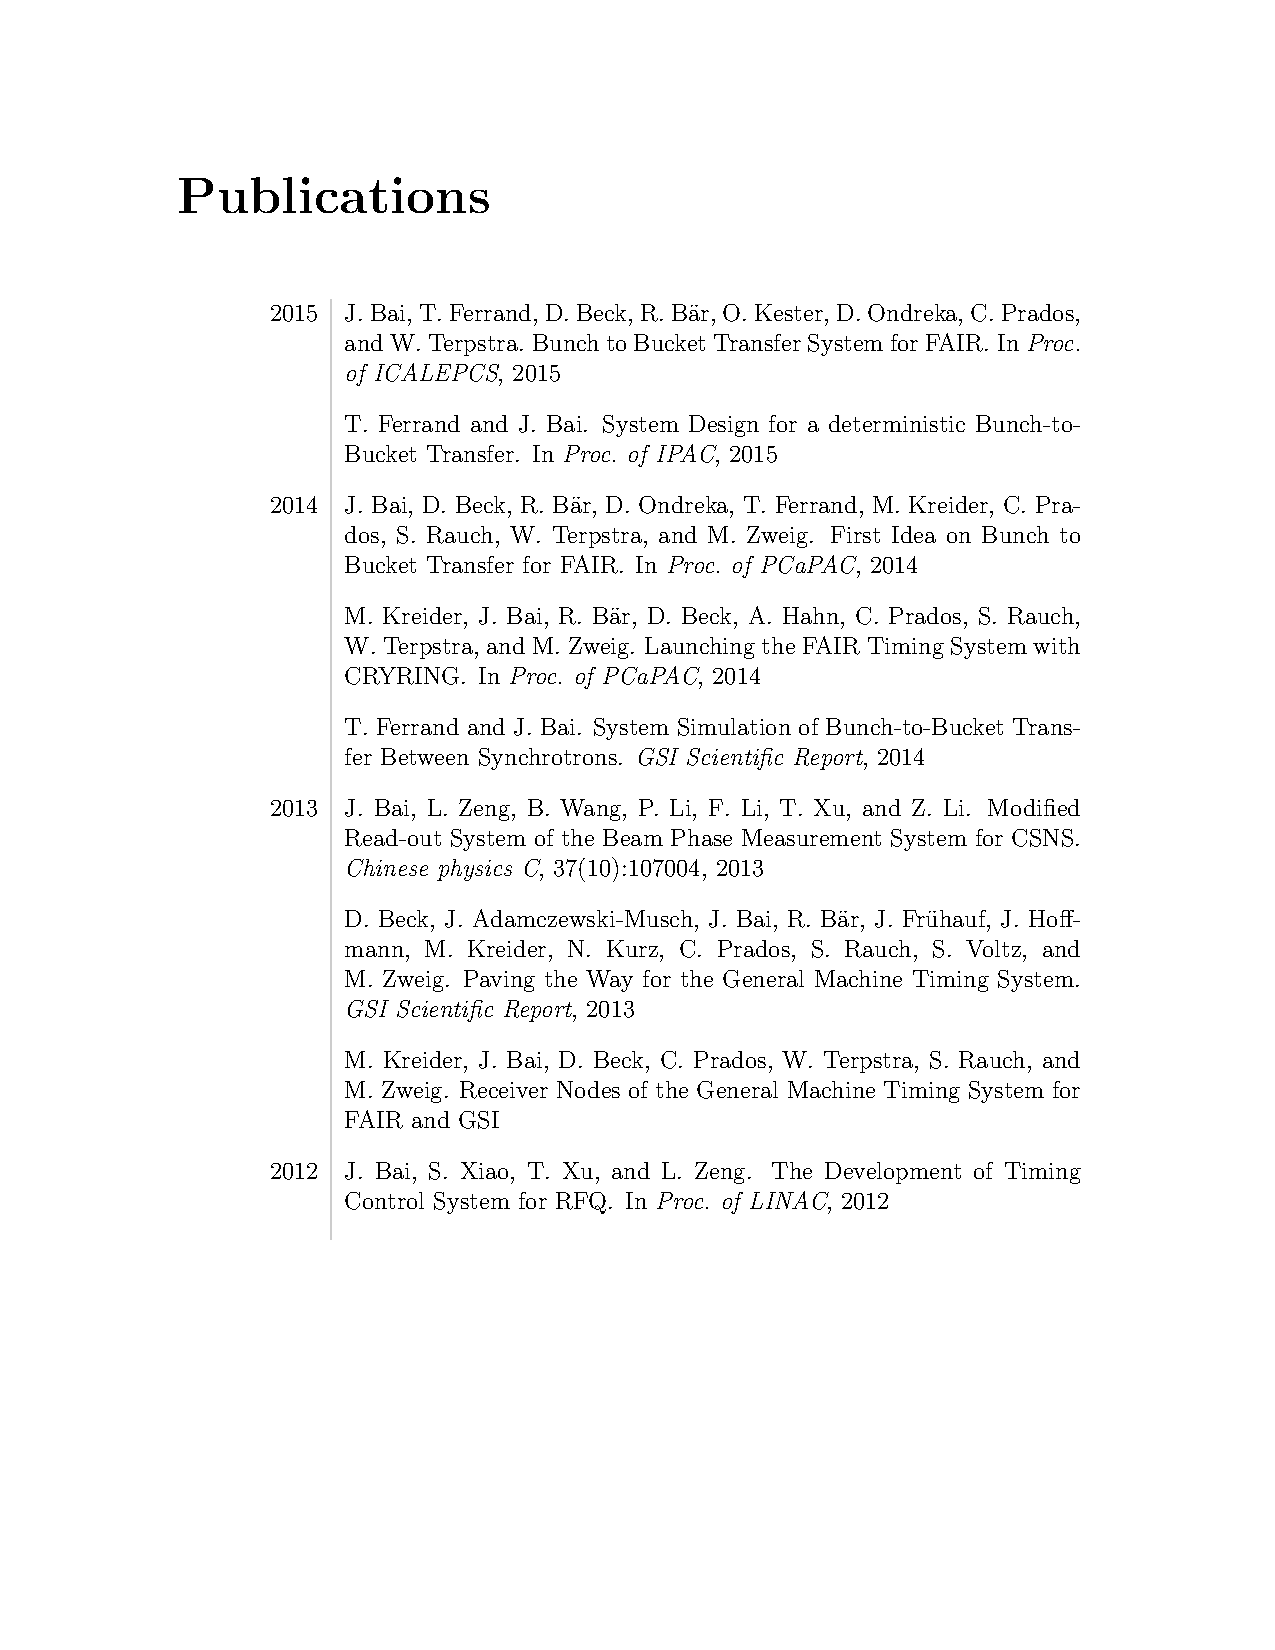
\includepdf[pages=-,pagecommand={}]{chapters/publication.pdf}

\renewcommand\chaptername{}
\pagestyle{empty}
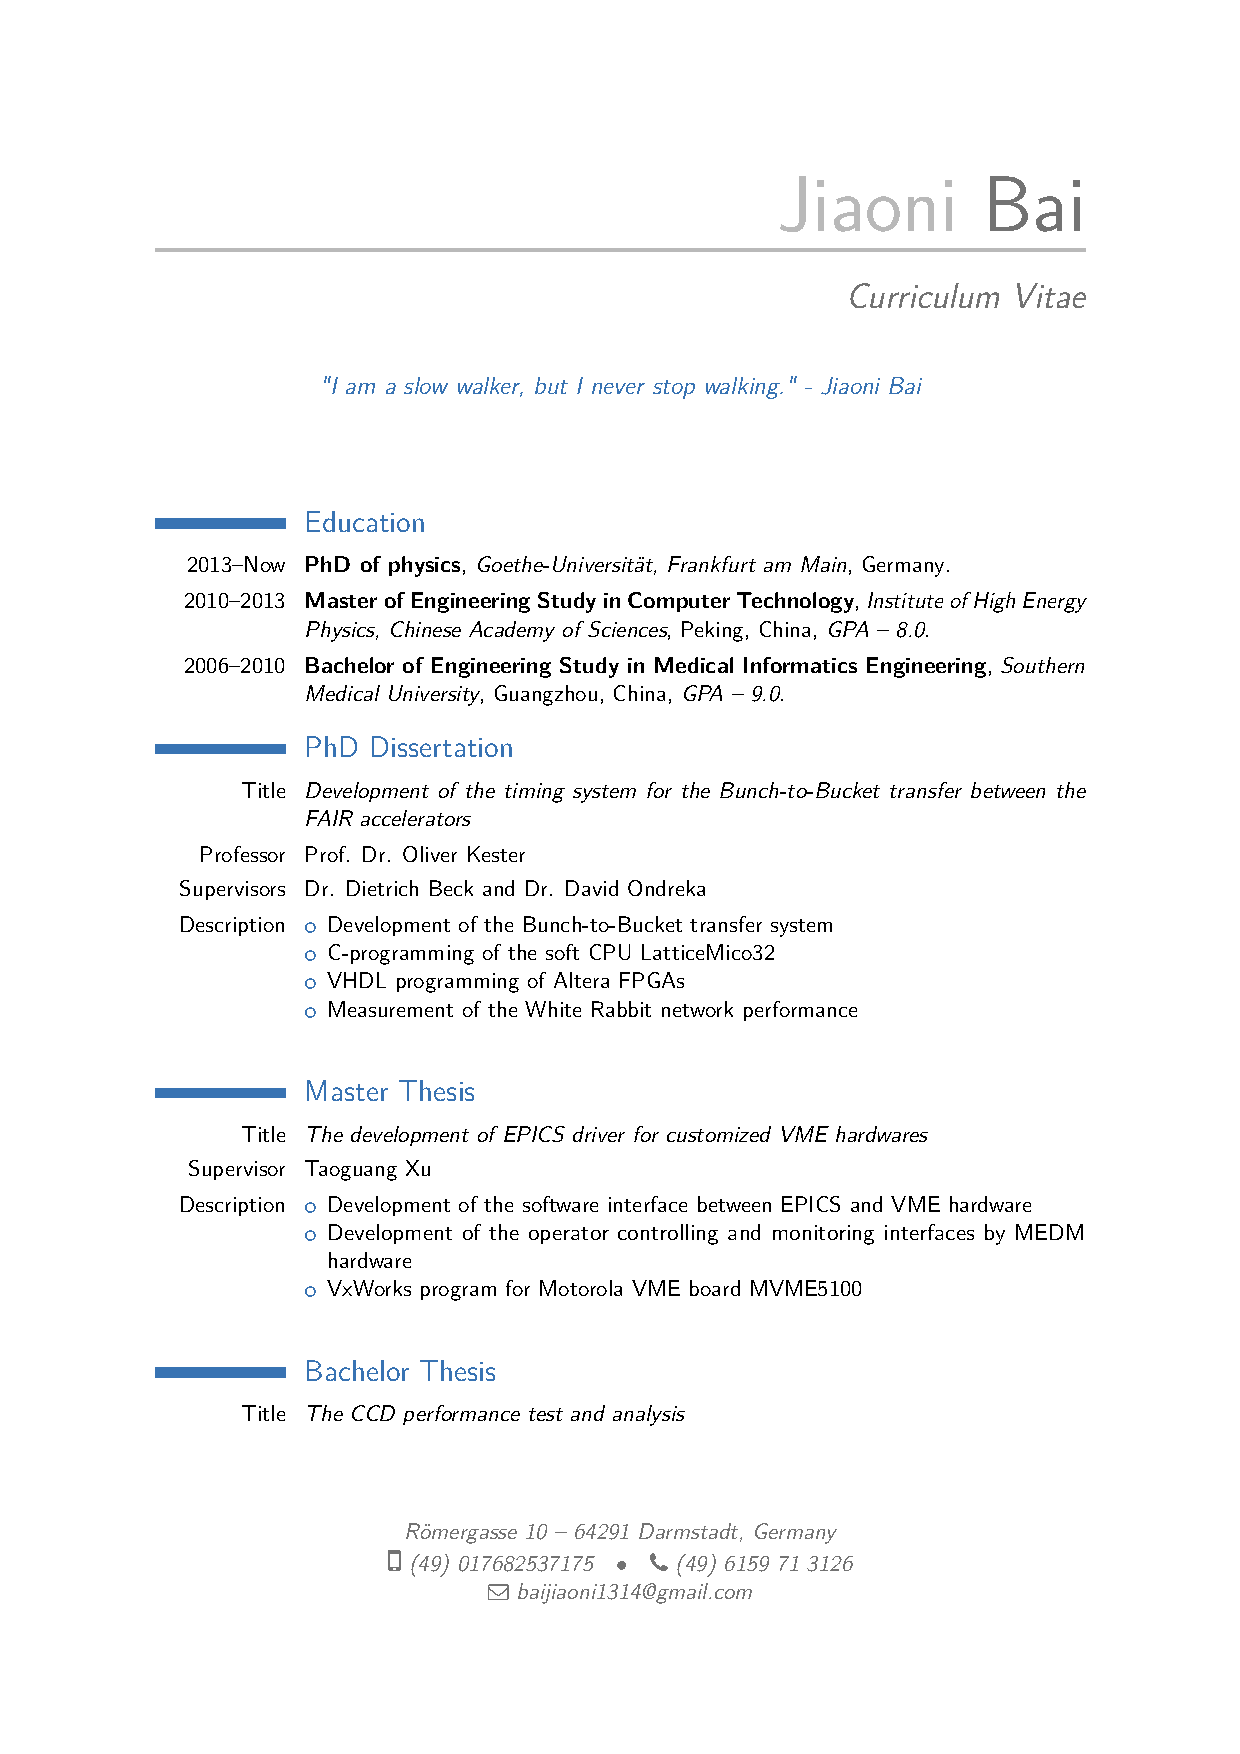
\includepdf[pages=-,pagecommand={}]{chapters/CV.pdf}
%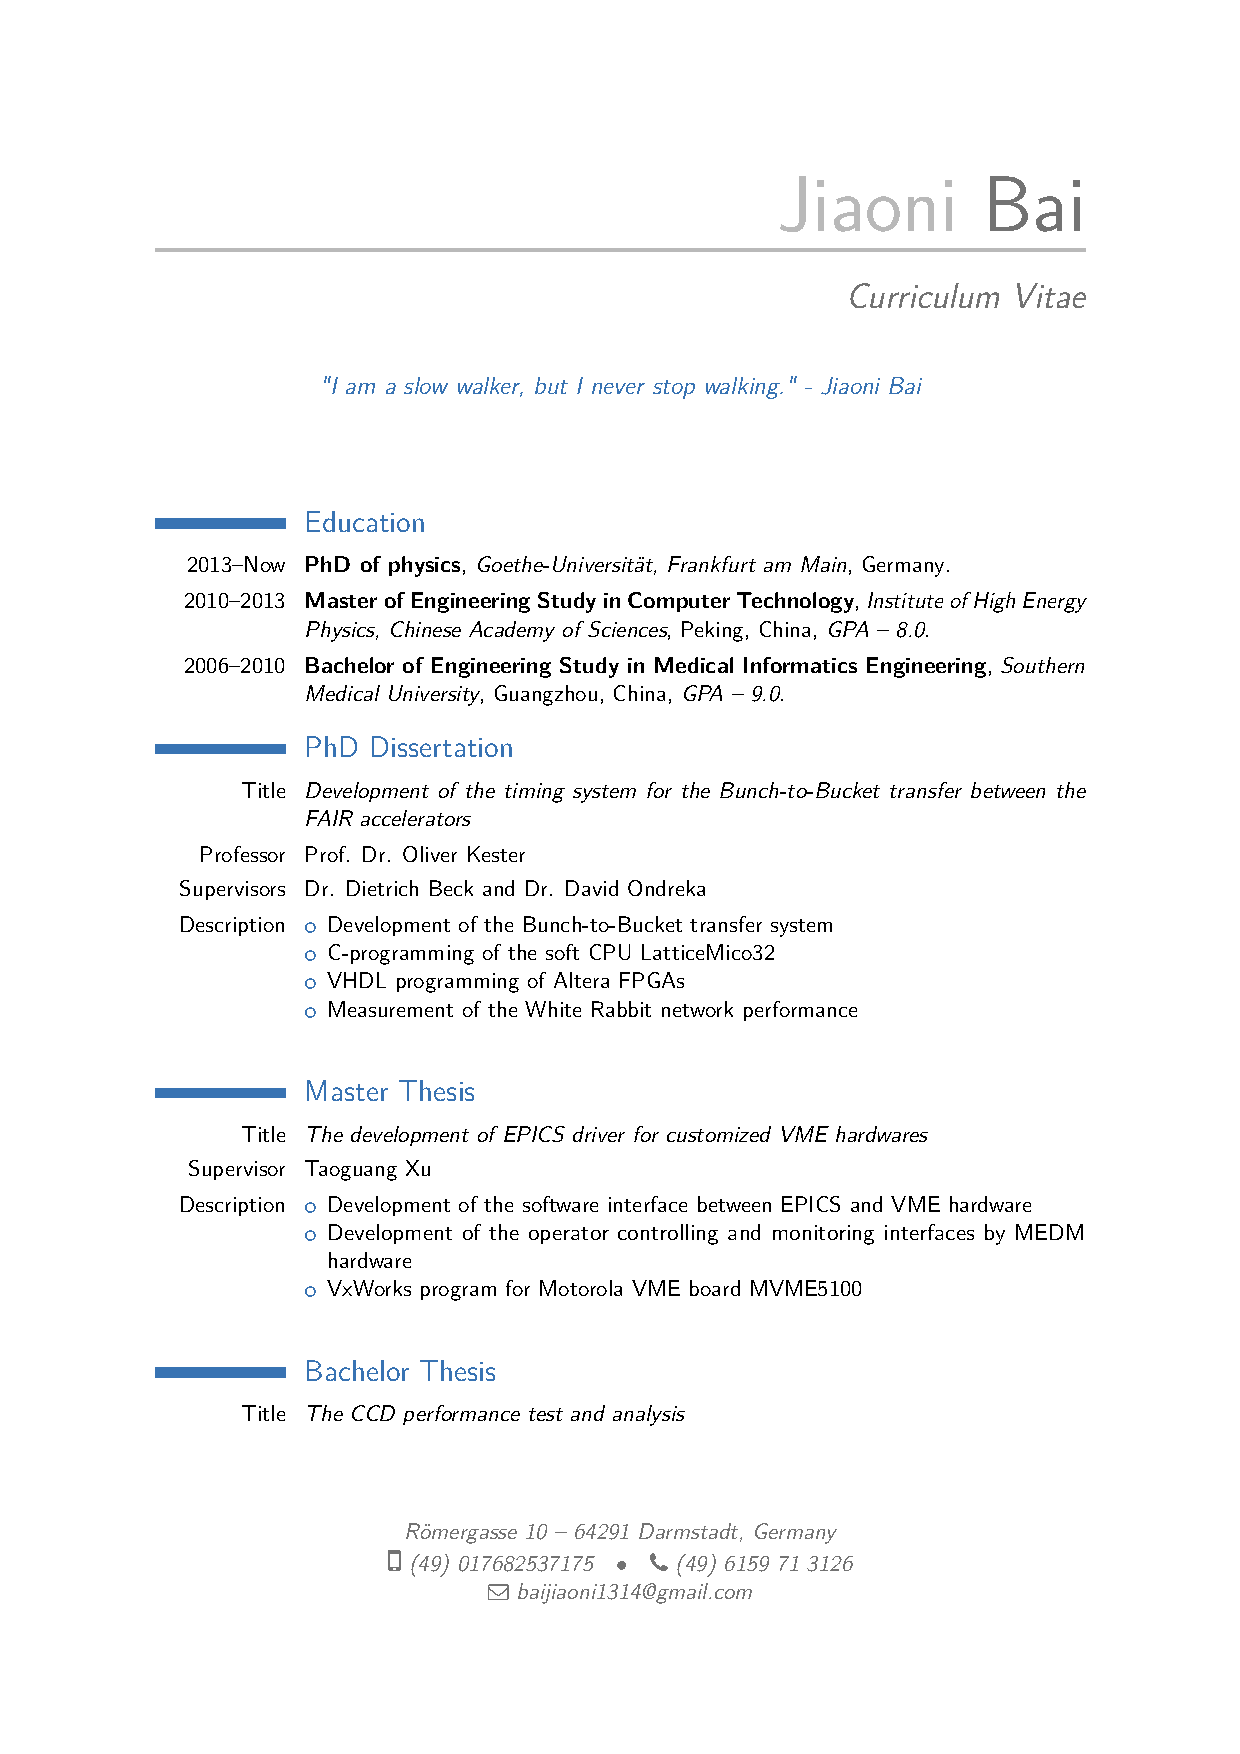
\includepdf{chapters/CV.pdf}

\end{document}

